%# -*- coding: utf-8-unix -*-
%%==================================================
%% thesis.tex
%%==================================================

% 双面打印
\documentclass[doctor, nofonts, openright, twoside, cs4size, submit]{sjtuthesis}
% \documentclass[bachelor, nofonts, openany, oneside, cs4size, submit]{sjtuthesis} 
% \documentclass[master, nofonts, review]{sjtuthesis} 
% \documentclass[%
%   bachelor|master|doctor,	% 必选项
%   adobefonts|winfonts,  	% 只测试了adobefonts,请使用adobefonts
%   oneside|twoside,		% 单面打印,双面打印(奇偶页交换页边距,默认)
%   openany|openright, 		% 可以在奇数或者偶数页开新章|只在奇数页开新章(默认)
%   cs4size|c5size, 		% 正文字号:小四、五号(默认)
%   review,	 		% 盲审论文,隐去作者姓名、学号、导师姓名、致谢、发表论文和参与的项目
%   submit			% 定稿提交的论文,插入签名扫描版的原创性声明、授权声明 
% ]


%% font settings
\usepackage{thesisfonts_external}

% 逐个导入参考文献数据库
\addbibresource{bib/thesis.bib}

%%%%%%%%%%%%%%%%%%%% my packages %%%%%%%%%%%%%%%%%%%%
% \addbibresource{bib/chap2.bib}
\usepackage{graphicx}
\usepackage{amssymb,amsmath,bm}
\usepackage{textcomp}
\usepackage{amsmath}
\usepackage{graphics}
\usepackage{epsfig}
\usepackage{multirow}
\usepackage{amsmath}
%\usepackage{url}
\usepackage{enumitem}
\usepackage{mathrsfs}
\usepackage{bm}
\usepackage{epstopdf}
\usepackage{array}
\DeclareMathOperator*{\argmax}{argmax}
\newcommand\Mark[1]{\textsuperscript#1}
\def\x{{\mathbf x}}
\def\L{{\cal L}}
\def\vec#1{\ensuremath{\bm{{#1}}}}
\def\mat#1{\vec{#1}}
\newcommand{\ue}{\mathrm{e}}
\usepackage{float}
\hyphenpenalty=5000

\begin{document}

%% 无编号内容:中英文论文封面、授权页
%# -*- coding: utf-8-unix -*-
\title{语音识别深度序列建模及解码}
\author{陈哲怀}
\advisor{俞凯教授}
\coadvisor{钱彦旻教授}
\defenddate{2018年12月1日}
\school{上海交通大学}
\institute{计算机科学与工程系}
\studentnumber{0140339029}
\major{计算机科学与技术专业}

\englishtitle{Deep Sequential Modeling and Decoding in Speech Recognition}
\englishauthor{\textsc{Zhehuai Chen}}
\englishadvisor{Prof. \textsc{Kai Yu}}
\englishcoadvisor{Prof. \textsc{Yanmin Qian}}
\englishschool{Shanghai Jiao Tong University}
\englishinstitute{\textsc{Department of Computer Science and Engineering} \\
  \textsc{Shanghai Jiao Tong University} \\
  \textsc{Shanghai, P.R.China}}
\englishmajor{Computer Science}
\englishdate{Dec. 1st, 2018}


\maketitle

\makeenglishtitle

\makeatletter
\ifsjtu@submit\relax
	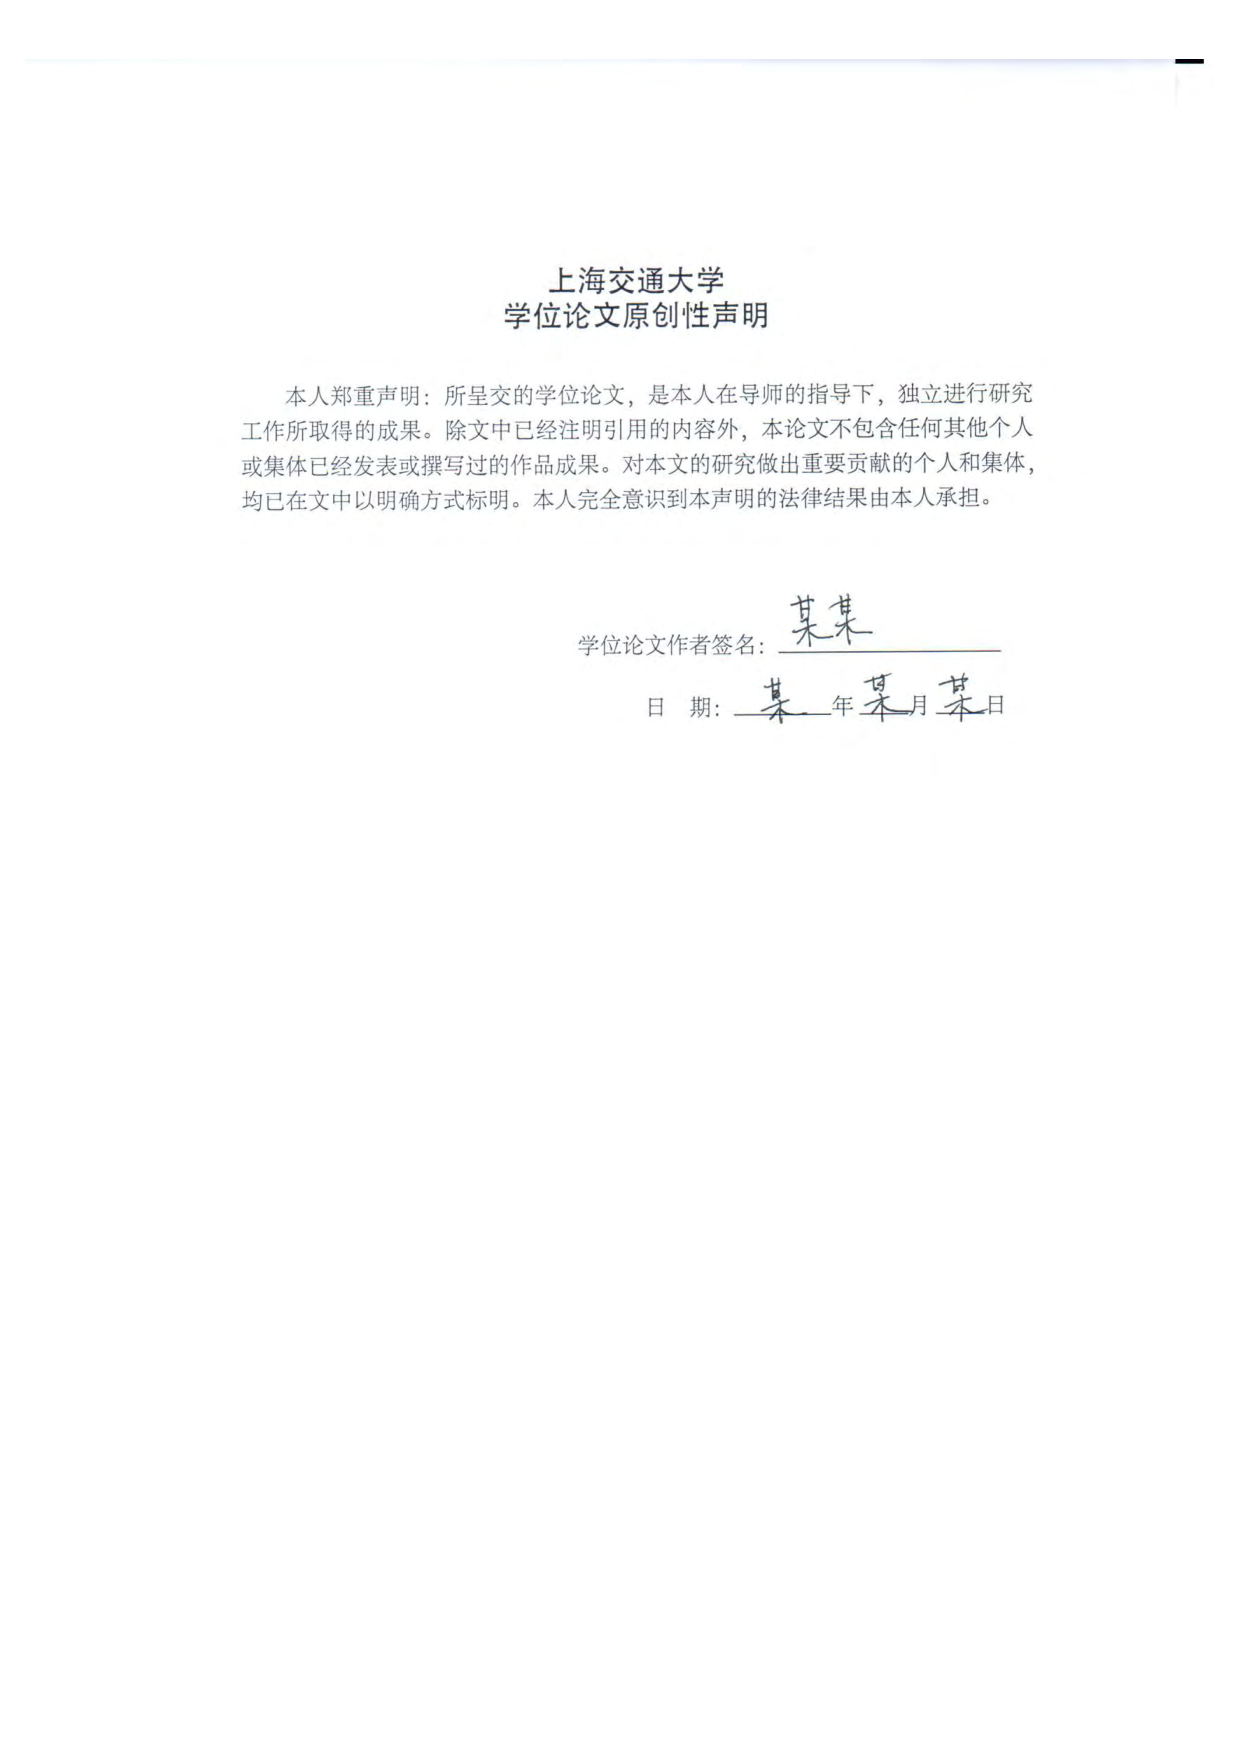
\includepdf{pdf/original.pdf}
	aaaaa
	\cleardoublepage
	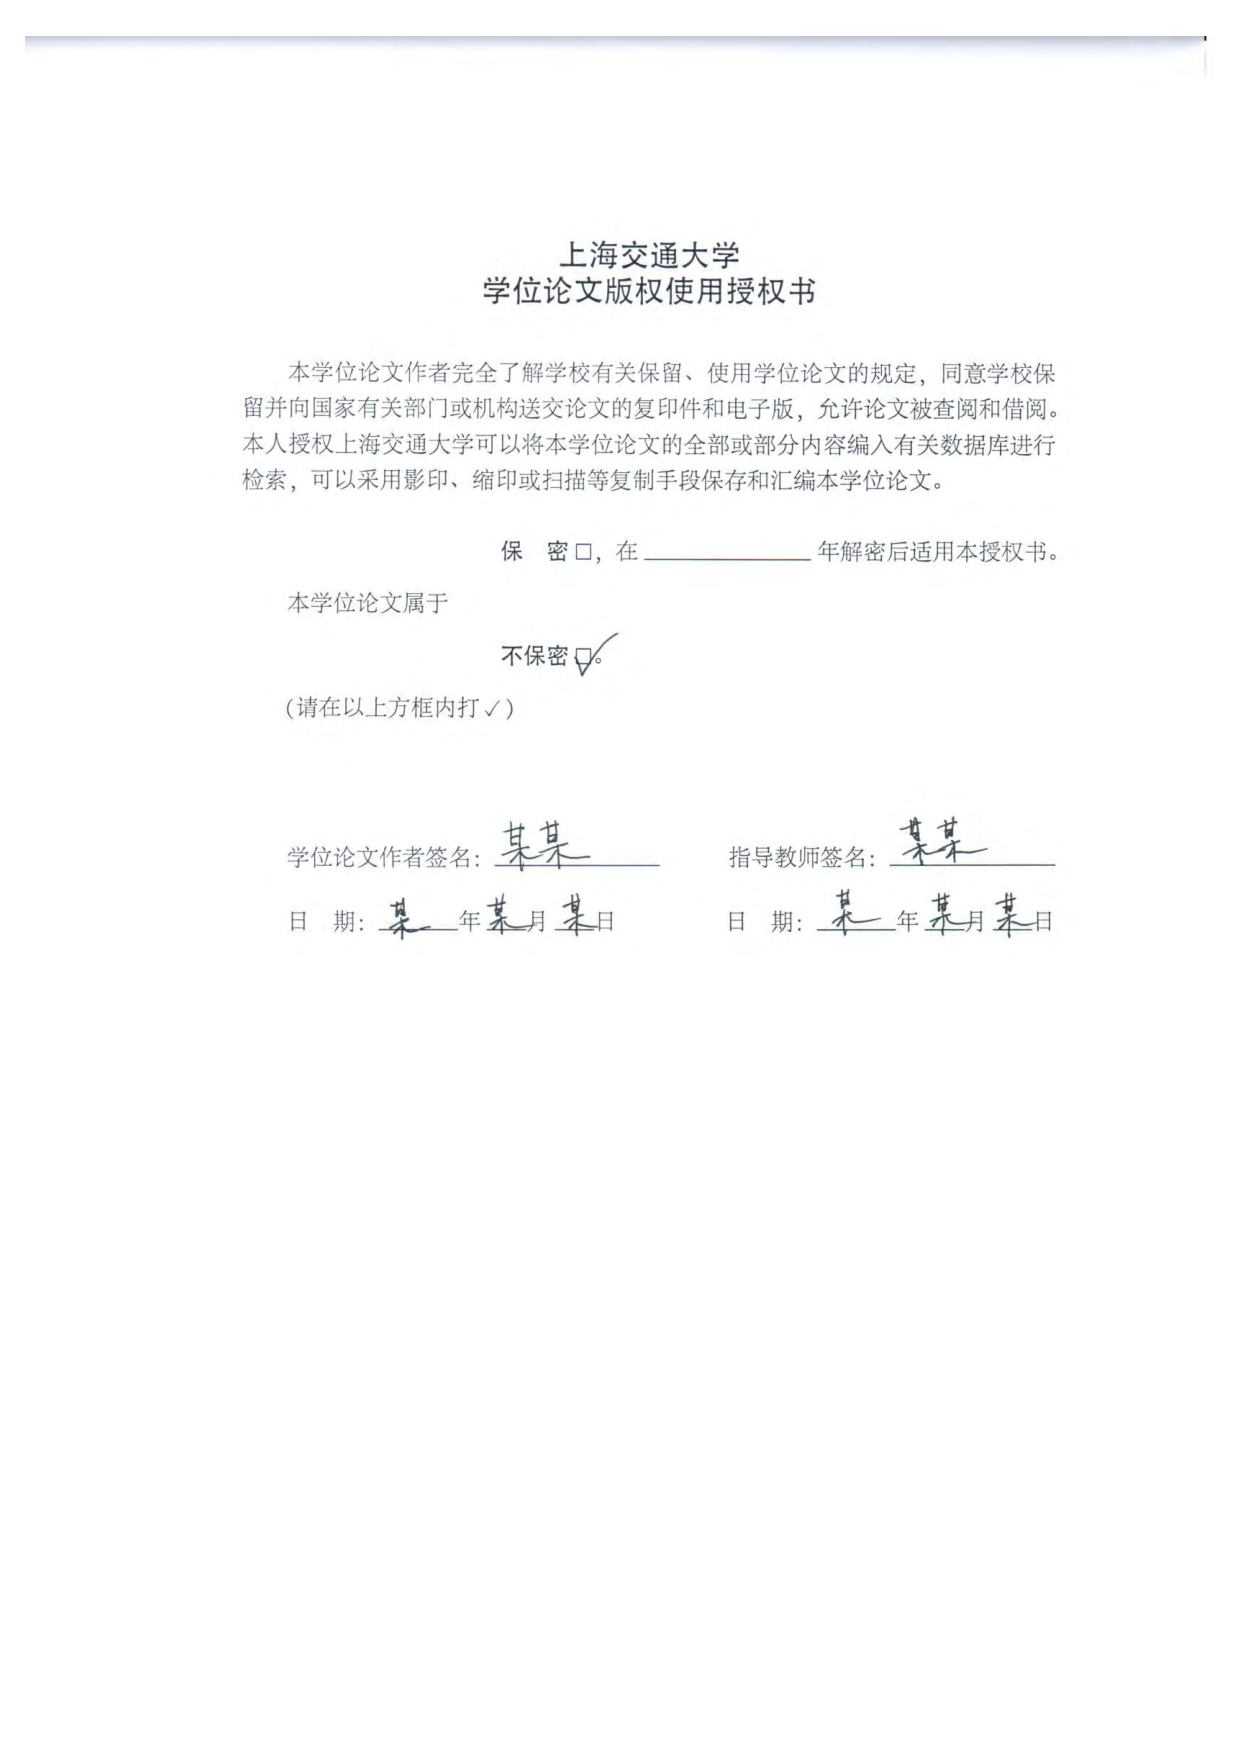
\includepdf{pdf/authorization.pdf}
	\cleardoublepage
\else
	\makeDeclareOriginal
	\makeDeclareAuthorization
\fi
\makeatother


\frontmatter 	% 使用罗马数字对前言编号

%% 摘要
\pagestyle{main}
%# -*- coding: utf-8-unix -*-
%%==================================================
%% abstract.tex for SJTU Master Thesis
%%==================================================

\begin{abstract}

语音识别中一个独有并且有趣的自然现象是声学序列和语言学序列的长度可变性,这使得语音识别需要同时建模两种序列之间的状态对齐与模式分类。
%
在训练阶段,一组带有已知标签的输入特征被提供给系统进行模型构建,{\em 序列建模}和{\em 模式分类}是前一问题的两大核心,这决定了语音识别系统可达到的识别精度的上限;而测试阶段,则基于特征序列和其它知识源如语言模型和字典进行模型{\em 搜索解码},这决定了识别速度和实际可达的识别精度。
%
近年来,深度学习模型被引入到语音识别的声学和语言建模当中替代传统分类器,显著改善了模式分类问题的精度。 但基于深度学习的语音识别并没有改变序列建模和搜索解码的本质。
本论文围绕深度学习背景下的序列建模和搜索解码技术展开了一系列探索和研究。

针对语音识别的精度,本论文从序列建模的角度改善语音识别的声学建模,首次针对关键词检测和多说话人重叠语音信号识别这两类非经典语音识别任务提出了序列建模准则和方案。
%
序列建模方法通常只在训练标准的大词汇连续语音识别模型时进行使用,但针对其它非传统识别任务的序列建模研究并不充分,这包括:关键词检测任务和多说话人重叠语音信号识别任务等。这类任务仍然是序列预测问题,但是却没有合适的训练准则和相应的设计,来充分优化分类器的序列建模能力。
为了将序列鉴别性训练引入关键词检测任务,核心难题是设计相应的竞争可能性建模方法。本论文提出采用无词图鉴别性训练框架来解决这一问题:隐性使用音素或半词单元的语言模型来建模。
另一方面,单通道多说话人混叠语音识别也属于序列级问题, 
我们提出了一种传统鉴别性训练技术变种,它在进行鉴别性训练的同时,也抑制输出通道上说话人跟踪错误。通过联合优化,迁移学习,序列鉴别性训练等方式,我们改善了原来语音分离、信号增强和语音识别的联合训练系统。

针对语音识别的速度,
本论文从解码搜索并行化和降低算法复杂度两个层面进行搜索解码算法加速:

一方面,本论文提出并行的解码搜索算法并在GPU上实现开源该套算法, 该框架可以显著加速现有推理搜索算法。
%
基于GPU的并行加速已成功应用于深度学习层面的模式分类任务,而语音识别解码搜索网络中多数边之间并不直接相关,也具有并行处理的可能性。但是,基于GPU并行计算的搜索网络(百亿边级别)解码研究仍然空白。
针对设计中的几大难点,本论文提出了如下解决方案:
本论文将维特比算法中的令牌合并操作实现为一个GPU并行计算中的原子操作以减少同步消耗;提出了动态负载均衡的方式以提高其多线程之间的利用率;重新设计了基于GPU并行计算的精确的词图生成和剪枝算法。
%
在Switchboard 上实验表明,本论文所提出的方法在取得完全一致的1-best和词图质量情况下,可以得到3-15倍的加速。除此之外,如果再进行多句子的并行处理,最终的加速比将达到46倍。
%所提出的离线解码器对语言模型和声学模型没有特别的限制,并且可以工作在各种架构的GPU上。

另一方面,本论文采用具有混淆区段建模(blank单元建模)能力的模型,系统地提出了标签同步算法,其通过一系列方法使得搜索解码过程从逐帧同步变为标签同步,从而加速解码。
当前主流的推理搜索方法是帧层面的维特比束搜索算法,在每一帧都要进行大规模的解码网络搜索,其算法复杂度很高,限制了语音识别的广泛应用。本论文提出对blank区段不进行搜索,将特征层面的搜索过程改变为标签层面,使得解码速率小于特征速率,即不必在每帧上都进行大规模搜索。
%具体来说,在标签搜索阶段,对帧层面声学模型的输出增加一步后处理过程, 得到对每个输出标签概率计算的近似值,再进行标签搜索。
与传统方法相比,该方法的优势是搜索空间更小,且搜索过程被大大加速。
本论文提出的一系列通用方法在隐马尔科夫模型和连接时序分类模型上得到了验证,取得大幅度语音识别解码速度改善。

本论文同时使能了大量语音识别的扩展应用。
上述标签同步算法所带来的搜索误差显著减小,由此产生高精度的音素词图,称为LSD音素词图。基于这种高精度词图,本论文进一步探讨标签同步解码算法的一些扩展应用,包括关键词检测,多识别任务统一置信度框架,以及端到端语音识别。
%
我们在关键词检测中,提出了一套基于编辑距离的后处理算法以引入音素混淆性,使系统更加鲁棒。
%
在高质量的LSD音素词图基础上,本论文进一步提出了两种置信度生成算法。
%
基于大幅加速的标签同步解码算法,本论文还提出了辅助归一化搜索空间的概念,并尝试使用这样的搜索空间来建模所有语音识别应用领域的置信度。 % and CM can be obtained in an unified framework
%而针对这样做在低功耗设备上带来的挑战,本论文采用标签同步解码来进行处理,由此带来了很大的效率改善。
%最终这一统一高效的置信度框架被应用于目前主流的多种ASR应用。
%
同时本论文还研究了将标签同步算法应用于直接建模输出序列形态学组合的端到端模型的方案。本论文使用模块化训练的思想来改善端到端模型建模,使其更易于使用外在知识源来训练每一个端到端模型的子模块,最终带来更好的模型准确度和更快的速度。
%值得注意的是,模型最后需要进行联合优化,因此最终在推理搜索阶段,模型仍然工作在端到端模式下。



总而言之,本论文围绕深度学习背景下的序列建模和解码搜索技术展开了一系列探索和研究。本论文提出的并行解码搜索技术与标签同步解码算法相结合,可以得到一个极大幅的速度提升;
再结合所提出的通用推理搜索和置信度方案,将得到一个低功耗、高性能的通用语音识别系统。本论文不仅在主要数据集上验证了相关算法,并且开源了部分算法系统。

\keywords{语音识别,序列建模,搜索解码,并行计算,标签同步解码,置信度,序列鉴别性训练}
\end{abstract}

\begin{englishabstract}

A unique phenomenon in human speech is the variable lengths in acoustic waves and linguistic words. Hence {\em automatic speech recognition} (ASR) requires both pattern classification and  state alignment modeling between input and output sequences, called {\em sequence prediction} problem. In the training stage, the model takes  acoustic features as the input and its labeling as the output, where {\em sequence modeling} and {\em pattern classification} are two keys, which determine the upper bound of a speech recognizer. In the inference stage, a speech recognizer is to find a sequence of labels whose corresponding acoustic and language models best match the input feature, called {decoding}, which determines the recognition speed and precision in real application. 
The most recent milestone of ASR is the application of deep neural networks (DNN) in acoustic and language modeling.
However, those successful applications are still based on the traditional formulation of speech recognition and only aim to improve the pattern classification above. In this thesis, the remaining sequence modeling and decoding problems are systematically investigated in the modern DNN based ASR.

We propose sequence modeling solutions of unconventional ASR tasks, keyword spotting (KWS) and overlapped speech recognition,  for the first time. Traditional sequence modeling research is usually conducted on the acoustic modeling of conventional speech recognition systems. Although keyword spotting and overlapped speech recognition are both inherently sequence prediction problems, they have not benefited from sequence modeling due to the lack of proper criteria and the difficulties of getting alternative sequence hypotheses for discriminative training. We propose to solve these problems in the lattice-free discriminative training framework. Namely, the competing hypotheses are efficiently modeled by phoneme or sub-word level language models. Moreover, this framework takes  speaker tracing and speech separation errors in overlapped speech into account. 
We propose a specific discriminative training formulation for overlapped speech recognition which also penalizes competing outputs from the overlapped speech. Our sequence modeling solutions achieve significant improvements in both unconventional ASR tasks, and show the potential to be combined with transfer learning and joint training.

For decoding, we propose algorithm speedups in two folds: parallelizing Viterbi search algorithm and decreasing algorithm complexity by label synchronous decoding. Firstly, we propose the {\em parallel Viterbi search algorithm}, implement it in GPU and make it open-sourced, achieving great speedups. Since most of the weighted finite state transducers (WFSTs) arcs in ASR are independent with each other, the search algorithm has the potential to be parallelized. However, the algorithm and implementation naturally work in serial and the previous rare trials have many limitations. We propose a series of solutions and redesign the algorithm:  token recombination as an atomic GPU operation in order to reduce synchronization overheads; dynamic load balancing strategy for more efficient token passing scheduling among GPU threads; the redesign of exact lattice
generation and lattice pruning algorithms for better GPU utilization. Experiments on the switchboard corpus show that the proposed method achieves identical ASR precision, while running 3 to 15 times faster. Additionally we obtain a 46-fold speedup with sequence parallelism and multi-process service (MPS) in GPU.

Secondly, based on confusion $\tt blank$ symbol modeling, we systematically propose {\em label synchronous decoding} (LSD) to transform the search process from frame level to label level and obtain significant speedups. The dominant decoding method nowadays is frame synchronous Viterbi beam search whose algorithm complexity is linear with the length of the acoustic waves. We propose  to transform the search process above from frame level to label level whose complexity is linear with the length of linguistic words. Namely, we utilize effective $\tt blank$ structure and apply efficient post-processing of $\tt blank$ during inference before doing Viterbi search. The proposed framework can be applied to both generative and discriminative sequence models. Experiments on the switchboard corpus show 2-4 times speedup in search without performance deterioration.

Moreover, significantly better quality of phone and word level lattices can be obtained from LSD methods above, called {\em LSD lattices}. We further improve a series of ASR systems based on LSD lattices, including keyword spotting, unified confidence measure framework, and acoustic-to-word (A2W) end-to-end modeling. In KWS, we introduce phoneme level confusion in inference stage by an efficient minimum edit distance  post-processing upon CTC lattices, to improve the precision and robustness. We propose two distinct confidence measure algorithms based on CTC lattices, showing prevalent quality. We propose auxiliary normalization graph upon CTC lattices  and take it as a unified search space for confidence measures in variant ASR applications. We utilize modular training to improve A2W modeling and make it better to utilize external knowledge sources. A LSD based joint training strategy is proposed to obtain better modeling precision and faster inference speed.

In conclusion, this thesis successfully improve the sequence modeling and decoding frameworks in the modern DNN based ASR. Tremendous speedups upon current speech recognizers can be obtained by combining the proposed parallel Viterbi search algorithm and label synchronous decoding. A low power-consumption and high quality unified ASR system can be built upon our works in sequence training and inference framework. The system is verified in variant datasets and some algorithms in the system are open-sourced.

\englishkeywords{\large Speech Recognition, Sequence Modeling, Decoding, Parallel Computing, Label Synchronous Decoding, Confidence, Sequence Discriminative Training}
\end{englishabstract}



%% 目录、插图目录、表格目录
\tableofcontents
\listoffigures
\addcontentsline{toc}{chapter}{\listfigurename} %将插图目录加入全文目录
\listoftables
\addcontentsline{toc}{chapter}{\listtablename}  %将表格目录加入全文目录
% \listofalgorithms
% \addcontentsline{toc}{chapter}{代码索引}  %将表格目录加入全文目录

%# -*- coding: utf-8-unix -*-
\chapter{主要符号对照表}
\label{chap:symb}

\begin{longtable}{rl}
\textbf{通用标记} \\
$s$ & 标量使用普通小写字母 \\
$\mathbf{v}$ & 列向量使用加粗的小写字母 \\
$\mathbf{X}$ & 矩阵使用加粗的大写字母 \\
$\mathcal{F}$ & 训练准则 \\
$\mathcal{M}$ & 模型参数 \\
$\mathbf{O}$ & 观测向量序列,$\mathbf{O}=[ \mathbf{o}_1, \dots, \mathbf{o}_T ]^\top$ \\
$\mathbf{o}_t$ & 第$t$帧的观测特征 \\
$\mathbf{w}$ & 词(标注或者假设)序列 \\
$a_{i,j}$ & 离散的状态转移概率 \\
$b_j(\mathbf{o})$ & 状态$j$的状态输出分布 \\
$m$ & 高斯成分的索引 \\
$\bm{\mu}^{m}$ & 第$m$个高斯成分的均值向量 \\
$\bm{\Sigma}^{m}$ & 第$m$个高斯成分的协方差矩阵 \\
$\mathbf{W}^l$ & 神经网络第$l$层的权重矩阵 \\
$\mathbf{b}^l$ & 神经网络第$l$层的偏置向量 \\
$\mathbf{x}^l$ & 神经网络第$l$层的激励向量 \\
$\mathbf{y}^l$ & 神经网络第$l$层的激活向量 \\

\textbf{数学标记} \\
$p(\cdot)$ & 概率密度函数 \\
$p(\cdot|\cdot)$ & 条件概率密度函数 \\
$P(\cdot)$ & 概率质量函数 \\
$\{ \cdot \}^{\top}$ & 向量或矩阵的转置 \\
$\{ \cdot \}^{-1}$ & 方阵的逆 \\


\textbf{英文缩写} \\
AM & 声学模型 \\
ASR & 自动语音识别 \\
CI & 上下文无关 \\
CD & 上下文相关 \\
CE & 交叉熵 \\
CMN & 倒谱均值归一化 \\
CVN & 倒谱方差归一化 \\
CN & 混淆网络 \\
DNN & 深度神经网络 \\
DSM & 鉴别式序列模型 \\
GMM & 混合高斯模型 \\
GPU & 图形处理芯片 \\
GSM & 生成式序列模型 \\
HMM & 隐马尔可夫模型 \\
KWS & 关键词检测 \\
LM & 语言模型 \\
LSD & 标签同步解码 \\
LSTM & 长短时记忆网络 \\
LVCSR & 大词汇连续语音识别 \\
MAP & 最大后验估计 \\
MSE & 均方差 \\
SGD & 随机梯度下降 \\
WER & 词错误率 \\
\end{longtable}
 % 主要符号、缩略词对照表

\mainmatter	% 使用阿拉伯数字对正文编号

%% 正文内容
\pagestyle{main}
%# -*- coding: utf-8-unix -*-
%%==================================================
%% chapter01.tex for SJTU Master Thesis
%%==================================================

%\bibliographystyle{sjtu2}%[此处用于每章都生产参考文献]
\chapter{绪论}
\label{chap:intro0}

\section{自动语音识别}
\label{chap:intro0-asr}


在日常生活中,语音是人与人之间交流最主要也是最有效方式。目前人机交互方式主要由键盘、鼠标和触摸屏来完成,随着移动设备的不断发展,过去的人机交互方式已经不再适用。用语音来进行人机交互能极大提高移动设备的易用性。使用语音来进行人机交互包含语音识别、语义理解、对话管理和语音合成等关键技术,而其中自动语音识别(Automatic Speech Recognition, ASR)作为整个闭环的入口无疑是最重要一环。
大词汇连续语音识别(Large Vocabulary Continuous Speech Recognition, LVCSR)是语音识别的经典传统任务,它的功能就是将人的语音转换为相应文本或者指令以用于后续的处理,这也是各种技术发展的核心测试任务;语音识别的另一大类应用是关键词检测(Keyword Spotting, KWS),它的目标是得到一个高准确度和高效率的识别器,用于检测特定的一些关键词在语音中的出现。

语音识别中一个独有并且有趣的自然现象是声学序列和语言学序列的长度可变性,这使得语音识别需要同时建模两种序列之间的状态对齐与模式分类。{\em 模式分类},{\em 序列建模},{\em 搜索解码}是语音识别中的三部分主要问题,下面将进行介绍。

\subsection{语音识别简史}
\label{chap:intro0-asr-history}

最早的语音识别系统出现在1952年贝尔实验室~\cite{davis1952automatic},这是一个只能进行孤立数字识别的系统。它没有使用通用计算机和任何统计机器学习的方法,只是一个精心设计端到端电路。现代的语音识别的基础开始于70年代,代表是隐马尔科夫(Hidden Markov Model, HMM)模型提出~\cite{baker1975dragon, jelinek1976continuous}。在这个模型中,观测特征的生成过程可以被两个条件概率所描述,发声的过程被描述为一个随机生成过程:状态转移概率和状态输出概率。HMM被用来对发声单元进行建模,发声单元包括音素,词或者句子。
在接下来的几十年中,随着高斯混合模型(Gaussian Mixture Model, GMM)被用于模拟状态输出概率和GMM-HMM理论的不断发展以及计算资源的不断改进,语音识别得到了显着的发展。语音识别任务也从简单的孤立词识别任务发展到大词汇量连续语音识别任务。从1988年开始,美国国家标准与技术研究所(National Institute of Standards and Technology, NIST)以及美国国防部高级研究计划局(Defence Advanced Research Project Agency, DARPA)联合组织几场对连续词汇语音识别评估。
这些评估极大地推动了语音识别研究的发展,并为语音识别设定了几个里程碑。语音识别词汇从1988年的资源管理任务中的900个单词改进到1993年华尔街日报中的20000个单词,实现了真正的词汇连续语音识别。不仅词汇量增加,而且语音识别的任务也朝着更现实的识别任务发展。例如,记录环境从干净的环境变为嘈杂的环境,并且记录工具从专用记录设备变为普通电话语音。随着记录环境变得更加复杂,优化的目标也从孤立的单词变为连续的单词序列预测。在20世纪90年代后期,在HMM的基础上,研究人员进一步提出了自适应和自适应训练技术~\cite{anastasakos1996compact,digalakis1995speaker,furui1989unsupervised,gales1998cluster,gales1998maximum,gales2001adaptive,gales2001multiple,gauvain1994maximum,kuhn1998eigenvoices,lee1996speaker,leggetter1995maximum,neumeyer1995comparative,pye1997experiments}来应对不断复杂的语音环境,以及序列鉴别性训练技术~\cite{bahl1986maximum,schluter2001comparison,chou1993minimum,goel2000minimum,juang1997minimum,povey2005discriminative,povey2001improved}来使用序列级准则进行模型优化。这两项技术是在深度神经网络(Deep Neural Network, DNN)提出之前对GMM-HMM系统在复杂环境下提升性能最核心的技术。苹果手机第一代Siri中使用的就是这些技术。

另一方面,语言模型在自动语音识别领域中,作为一个声学模型重要的“帮手”而存
在。
语言模型的作用是对一句话中有多大可能在自然语言语料之中出现进行建模。
统计语言模型是在词语序列(即句子)层面的一个概率分布,比如说在给定 m 个词的句子中,语言模型的任务是获取整个句子的概率表示。
%
N-gram 语言模型\cite{chen1999empirical} 由其简单和有效而被广泛地使用,但是由于模型特性,其受到了“维度诅咒”,即在现实语料中历
史 gram 呈几何性增长,不可能被一一充分地建模。不同的“平滑”手段被提出来解决这一个问题,使得语言模型质量得到了显著改善。

最早在20世纪90年代~\cite{bourlard1989continuous,bourlard1992cdnn,bourlard2012connectionist},研究人员提出了一种使用神经网络(Neural Network, NN)对隐马尔科夫模型中的状态输出概率进行建模的方法。但是,由于当时缺乏计算资源和数据,该框架没有达到比GMM-HMM系统更好的性能。随着摩尔定律继续有效,今天的计算机计算能力已经从二十年前实现了巨大的飞跃。图形处理单元(Graphics Processing Units, GPU)使计算机能够更快地执行并行计算,从而可以训练更强大的模型。随着越来越先进的移动互联网和云计算,现在可以更轻松地收集足够的训练数据。这些因素都使得深度神经网络(Deep Neural Network, DNN)在今天可以被成功地训练。深度神经网络-隐马尔科夫模型 (DNN-HMM)的提出是对GMM-HMM框架的一次变革,令语音识别性能再次获得了巨大的提高,真正走出了实验室研究层次~\cite{ASRBook-Yu2014,CD-DNN-HMM-dahl2012,DNN4ASR-hinton2012,qian2016very,TDNN-peddinti2015,Deepspeech2-amodei2015,LACE-yu2016,xiong2017microsoft}。谷歌、微软、苹果等国际IT巨头近年都推出了以语音识别为核心技术的商业级产品。


单词错误率(Word Error Rate, WER)是衡量语音识别系统质量的重要指标。给定正确注释和语音识别系统的解码结果,将单词错误率定义为两个单词序列之间的编辑距离,值越小越好。图~\ref{fig:WER}反映是截止到2009年深度神经网络出来之前NIST赞助的各个语音识别任务词错误率变迁。其中横坐标是时间,纵坐标是词错误率,每一条折线代表着一项语音识别任务。
\begin{figure}[ht]
  \centering
    \captionstyle{\centering}
    \centering
    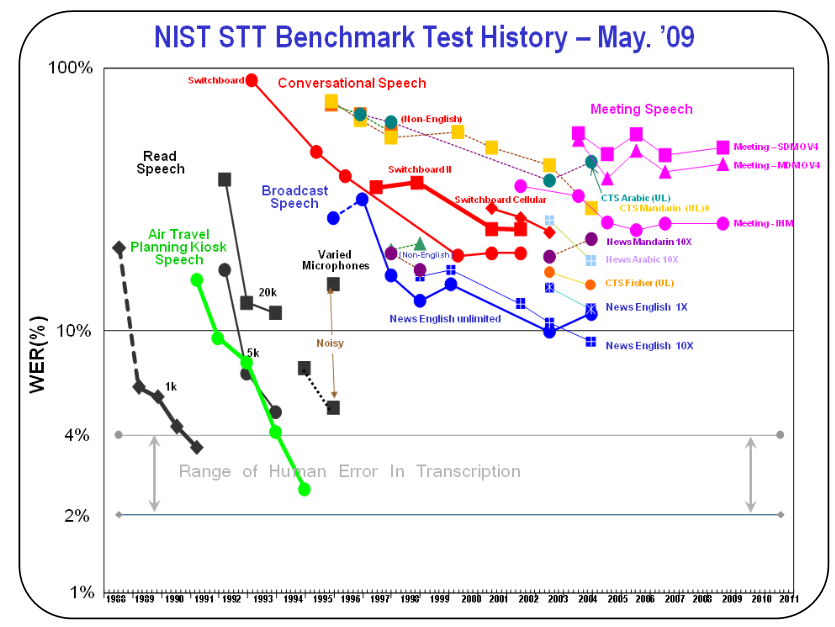
\includegraphics[width=.7\textwidth]{WER.png}
    \bicaption[fig:WER]{}{语音识别词错误率变迁图(截止2009年)}{Fig}{History of WER on several tasks (until 2009)}
\end{figure}

最早的任务是在干净的环境中的阅读语音的识别。随着GMM-HMM模型的改进与人类的识别率相同,到了20世纪90年代,任务逐渐接近日益复杂的现实环境。仅使用GMM-HMM模型,单词错误仍然很高。其中一个标志性的任务是Switchboard,它是一种电话语音识别。语音识别任务中最大的两个困难是:第一,语音信号是高度非线性信号;第二,声学环境(扬声器,噪声等)对语音信号有很大影响。从图中可以看出,任务场景越向右开,就越难。在21世纪初,学者们分别研究了序列鉴别性训练(序列建模)和自适应方法来解决这两个问题。可以看出,Switchboard的字板错误率已大大降低。2010年,微软学者提出使用深度神经网络对语音信号进行建模。神经网络的高非线性与语音信号非常吻合,并且Switchboard字的错误率进一步降低。由于DNN-HMM框架是GMM-HMM框架的一次革命,序列鉴别性训练和自适应技术是独立于框架的两个技术方向。因此,他们在新框架下有了新的发展空间。近年来,基于深度神经网络序列的鉴别性训练和自适应技术已成为新时代语音识别领域的核心研究内容。本文主要研究基于深度神经网络的序列建模技术。

另一方面,语音识别既是模式分类问题又是相应的推理搜索问题。前一个问题确定了语音识别系统可以实现的识别准确度的上限;在给定模型的情况下,后一问题研究如何使输入语音与模型匹配并推断最佳识别结果,其确定识别速度和实际可达到的识别准确度。近年来,DNN-HMM框架为代表的深度学习模型被引入到语音识别声学和语言建模中以取代传统的分类器,但分类器之外的推理搜索问题和前文提到的序列建模没有根本改变。
基于加权有限状态机(Weighted Finite State Transducer, WFST)的推理搜索问题静态搜索空间构造技术~\cite{mohri2002weighted}和帧同步维特比(Viterbi)网络搜索算法~\cite{forney1973viterbi}是目前性能最好的解决方案。

\subsection{语音识别架构}
\label{chap:intro0-asr-framework}


在迄今为止最为成功的基于统计的语音识别框架中,语音识别过程可以被抽象为如下数学公式:

\begin{equation}
    \label{eq:asr}
    \mathbf{w}^* = \arg \max_{\mathbf{w} \in \mathcal{H}}P(\mathbf{w}|\mathbf{O})
\end{equation}

即在所有可能的候选序列$\mathcal{H}$中寻找最大后验概率$P(\mathbf{w}|\mathbf{O})$对应的词序列$\mathbf{w}^*$。其中$\mathbf{w}=\left[ w_1, ..., w_n \right]^\top$是词序列,$\mathbf{O}=\left[ \mathbf{o}_1, ..., \mathbf{o}_T \right]^\top$是特征向量序列。


在LVCSR中,直接对后验概率$P(\mathbf{w}|\mathbf{O})$建模是比较困难的,这个问题可以通过贝叶斯公式转换成条件似然$p(\mathbf{O}|\mathbf{w})$,先验$P(\mathbf{w})$和$p(\mathbf{O})$。因为边缘分布$p(\mathbf{O})$在解码过程中与假设词无关,所以可以忽略掉。在剩下部分中,$p(\mathbf{O}|\mathbf{w})$被称为声学模型,$P(\mathbf{w})$被称为语言模型。声学模型用做建模子词单元生成特征序列的概率的,语言模型描述的是局部语法和整句的语言语义信息。



\begin{eqnarray*}
    \centering
    \mathbf{w}^* &=& \arg \max_{\mathbf{w} \in \mathcal{H}}P(\mathbf{w}|\mathbf{O}) \\
    &=& \arg \max_{\mathbf{w} \in \mathcal{H}} \frac{p(\mathbf{O}|\mathbf{w})P(\mathbf{w})}{p(\mathbf{O})} \\
    &\propto& \arg \max_{\mathbf{w} \in \mathcal{H}} p(\mathbf{O}|\mathbf{w})P(\mathbf{w}) \\
\end{eqnarray*}


在关键词检测中, 既可以采用上述的方式进行贝叶斯公式转换,此时将$P(\mathbf{w})$定义为各个关键词序列出现的先验概率;也可以不采用贝叶斯公式,直接对后验概率$P(\mathbf{w}|\mathbf{O})$进行建模。

\begin{figure}[!htp]
  \centering
    \captionstyle{\centering}
    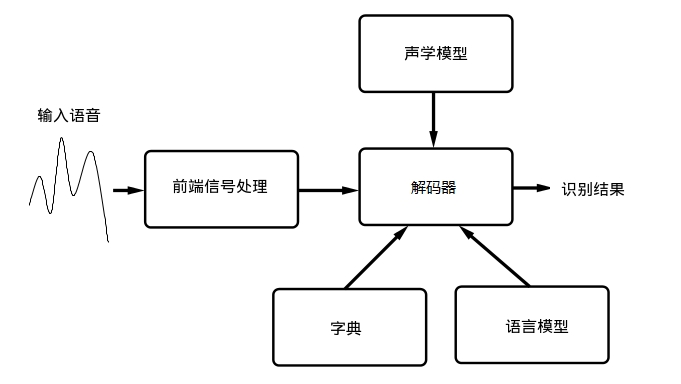
\includegraphics[width=.9\textwidth]{asr.png}
    \bicaption[fig:asr]{}{语音识别框架}{Fig}{Framework of an automatic speech recognition system}
\end{figure}

图~\ref{fig:asr}是对当前流行语音识别系统的框架描述,它主要由四个部分组成,包括前端信号处理、声学模型、语言模型和解码器。
\begin{itemize}
    \item 前端信号处理:原始模拟信号首先由输入设备转换为数字信号。前端信号处理部分负责从数字化语音中提取鲁棒声学特征信息,主要包括多麦克风阵列噪声降低和人耳听觉声学特性的提取。详细内容将在章节~\ref{sec:feat_extra}中介绍。
    \item 声学模型(Acoustic Model, AM): 声学模型是语音识别系统中最重要的模型之一。声学模型的好坏可以直接决定了语音识别系统的性能,也是本论文研究重点之一。声学模型建模的是给定词序列生成出来的所观测到的特征向量序列条件概率$p(\mathbf{O}|\mathbf{w})$,目前主流的语音识别系统通常是使用隐马尔科夫模型(Hidden Markov Model, HMM)来做为声学模型的。在HMM中,存在一个概率分布熵被称为状态输出概率,这个概率可以使用高斯混合模型来得到建模,也可以通过深度神经网络来建模。使用前者语音识别系统可以被称为GMM-HMM系统,使用后者被称为混合系统(DNN-HMM)系统。具体内容将在章节~\ref{sec:hmm}和章节~\ref{sec:dnn_hmm}中详细介绍。
    \item 语言模型(Language Model, LM): 过去了数十年,N元组模型(n-gram)是最主要的使用语言模型~\cite{good1953population,katz1987estimation,brown1992class}。近几年,基于深度神经网络语言模型也逐渐开始得到发展并取得了巨大性能的提升~\cite{mikolov2010recurrent,mikolov2012statistical}。
    \item 解码器及搜索(Decoder): 解码器功能是对声学模型中计算出的声学特征上的概率和语言模型计算出的语言概率去进行组合来得到最大概率的词序列。目前主流的解码算法是去使用基于动态规划思想的维特比算法(Viterbi Algorithm),将在第\ref{sec:decode}章节中详细介绍。
\end{itemize}

\section{语音识别中的序列建模}
\label{chap:intro0-seq-model}

语音识别是一种序列预测问题,在语音识别中一个独有并且有趣的自然现象是声学序列和语言学序列的长度可变性。
序列模型正是被提出用来解决两个序列之间的关联性。
依据序列的不同建模方式,目前有两种不同的序列鉴别性训练方法,一种针对生成式序列模型 (Generative Sequence Model, GSM) 比如上文介绍的HMM以及其相应的深度学习系统;另一种则针对鉴别式序列模型 (Discriminative Sequence Model, DSM) ,比如 连接时序分类模型 (Connectionist Temporal Classification, CTC) 或者 encoder-decoder 模型。 
在这些序列模型中,除了需要研究如何将各种基于深度学习的模型方法应用到逐帧分类当中,使用序列级的鉴别性训练准则来强化模型的序列分类能力,也被证明是取得业界最好的大词汇连续语音识别系统的关键。

针对GSM,使用隐马尔科夫模型, 在进行序列鉴别性训练之前,需要首先使用贝叶斯公式计算序列后验概率。根据贝叶斯公式,可以将序列后验概率展开为标注序列的声学模型概率和语言模型概率两项,以及分母项针对所有可能的序列的概率进行求和的边缘概率项,共三部分。由于语音识别的搜索空间巨大,一般研究中通常采用词图对边缘概率项的可能序列进行限制。而该部分词图的质量也是取得良好性能的关键之一。
%
DSM则是直接对序列后验概率进行估计的一类模型,如CTC是一个典型的例子~\cite{graves2006connectionist,huang2018ctc}。序列鉴别性准则定义为所有可能的CTC标签序列的概率求和,作为最终的优化方向。一个额外的$\tt blank$ 单元被引入到逐帧展开公式中以建模语音信号的混淆区段。

上述基于词图的序列建模方法存在几方面缺陷:词图构建引入了一个额外的步骤,使得词图更新频度和词图质量需要进行额外的权衡;逐句生成的词图导致序列建模过程中较难进行多句并行训练,而并行训练是目前最主流的加速模型训练的方式,训练速度的问题导致目前难以进行大规模的序列建模训练;该框架基于一个预训练的种子模型,因此种子模型的质量一方面关系到目前流行的深度学习模型的最终优化结果,另一方面也影响标签序列逐帧强制对齐的精度,从而影响最终序列建模训练的结果。

另一方面,序列建模方法通常只在训练LVCSR模型时进行使用,但针对其它非传统识别任务的序列建模研究并不充分,这包括:关键词检测任务和多说话人重叠语音信号识别任务等。这类任务仍然是序列预测问题,但是却没有合适的训练准则和相应的设计,来充分优化分类器的序列建模能力。因此这些领域近几年的进展主要仍然来自于深度学习本身所带来的更好的逐帧分类能力。

因此,尽管基于深度学习模型的序列建模研究已经取得了一定进展,但是更好、更通用的序列建模框架,以及针对更多语音识别任务的拓展,仍是亟待研究的问题。


\section{语音识别中的解码搜索}
\label{chap:intro0-inf}

语音识别技术虽然相比多年以前已经有了长足的进步,但是在实际应用中还有很多困难需要处理。其中一个最主要难题就是语音识别推理搜索问题。

%TODO1: 做什么事情
语音识别既是模式分类问题又是相应的推理搜索问题。前一个问题在数学上表示和描述了各种语音和语言现象,并且基于统计学习模式分类框架执行建模,该框架确定了语音识别系统可以实现的识别准确度的上限。在给定模型的情况下,后一问题研究如何使输入语音与模型匹配并推断最佳识别结果,其确定识别速度和实际可达到的识别准确度。在语音识别的推理搜索阶段,解码器功能组合声学模型以计算声学特征概率和语言模型计算的语言概率以获得最大概率词序列。
在语音识别推理搜索阶段,解码器是语音识别系统的核心和灵魂,所有信息都收集在这里。它将来自不同来源,不同层次和不同性质的知识和信息联系起来,以便它们相互补充并获得正确的语音识别结果。因此,如何有机地整合各种不同的信息是解码网络和解码算法设计中必须仔细研究和解决的问题。
从解码器功能的角度来说,它不仅是语音识别研究中各种理论,模型和算法的验证。
正确性和准确性的基本实验平台也是构建实际系统的基础所在。因此,在解码器的设计中必须平衡研究的便利性和工程的实际应用。


%TODO3: 近来深度学习下发展现状和缺陷
近年来,深度学习模型被引入到语音识别声学和语言建模中以取代传统的分类器,显着提高了模式分类问题的准确性。在基于深度学习语音识别中,推理搜索问题没有根本改变,因为深度学习只是取代了分类器。
基于加权有限状态机的推理搜索方法,即静态搜索空间构造技术~\cite{mohri2002weighted}和帧同步维特比(Viterbi)网络搜索算法~\cite{forney1973viterbi},仍是目前性能最好的解决方案。
WFST是一组加权有限状态机表示的状态图跳转信息,语音信号的识别各模型组件可以分别构建成一组WFST。
当各个知识源WFST组件被构建完毕以后,可以利用WFST合成算法和优化算法将各组件最后进行合并和最终优化。最终生成的WFST包含了所有的知识源,维特比搜索就在它上面逐帧进行。
该方法虽然比传统动态解码技术更高效,但仍存在一系列显著缺陷:
\begin{enumerate}
\item 
该种方案基于传统的混合高斯-隐马尔科夫模型(GMM-HMM)的声学模型和N元文法(N-gram)的语言模型而提出,针对目前性能最好的基于深度学习的声学模型和语言模型的研究并不充足,如何将新型的声学和语言模型引入该框架;如何充分发挥模型性能的同时改善推理速度;如何基于多知识源给出可靠的推理置信度算法,都是有待解决的问题。
\item 
该种方案基于对语音识别中各知识源(声学、语言、语义等)进行搜索空间的预先构建及整体优化,导致最终得到的搜索空间巨大,包括离线构建、在线使用、动态修改等各环节算法的计算量和内存消耗都非常大,是阻碍语音识别应用场景扩展的一个重要原因。旨在解决该问题,针对新型声学和语音模型的搜索空间整体优化研究尚不充分,而基于推理中间状态对搜索空间进行动态优化的研究几乎处于空白。
\item 目前,语音识别系统基于多知识源建模结果,并对输入音频进行推理搜索。建模和推理搜索过程非常复杂,知识来源的划分依赖于强大的先验知识。大规模或非标记语音数据收集以及基于并行的深度学习技术使得构建直接模拟语音数据和文本序列的端到端模型及其相应的识别和推理搜索算法成为可能。当前的解码框架没有这种设计。
\end{enumerate}

因此,尽管基于深度学习模型,加权有限状态机和基于帧的维特比网络搜索算法的深度学习已经发展到基本可用水平,但是精度仍然不能满足人类之间的正常交流要求。速度限制也使得语音识别无法在低成本和低功耗的解决方案上工作,这些一起阻碍了语音识别技术的大规模商业应用。


\section{论文主要内容、创新点及组织结构}
\label{chap:intro0-thesis}


本论文围绕深度学习模型的序列建模和解码,针对上面探讨的诸多研究缺陷,展开了一系列探索和研究,主要涉及
了非传统识别任务的序列建模,基于GPU并行计算的搜索速度优化,基于标签同步解码搜索空间优化,标签同步解码的扩展应用等内容。

\begin{enumerate}
\item 本论文针对关键词检测和多说话人重叠语音信号识别这两类非传统语音识别任务提出了序列建模方案。

序列建模方法通常只在训练LVCSR模型时进行使用,但针对其它非传统识别任务的序列建模研究并不充分,这包括:关键词检测任务和多说话人重叠语音信号识别任务等。这类任务仍然是序列预测问题,但是却没有合适的训练准则和相应的设计,来充分优化分类器的序列建模能力。
为了将序列鉴别性训练引入关键词检测任务,核心难题是设计相应的竞争可能性建模方法。本论文提出采用无词图鉴别性训练框架来解决这一问题:隐性使用音素或半词单元的语言模型来建模。
另一方面,单通道多说话人混叠语音识别也属于序列级问题, 因此序列鉴别性准则将有助于这样序列分类问题。
我们提出了一种传统鉴别性训练技术变种,它在进行鉴别性训练的同时,也抑制输出通道上说话人跟踪错误。通过联合优化,迁移学习,序列鉴别性训练等方式,我们改善了原来语音分离、信号增强和语音识别的联合训练系统。

    \item 
本论文提出并行的解码搜索算法并在GPU上实现开源该套算法, 该框架可以显著加速现有推理搜索算法。

语音识别解码网络中多数WFST边之间并不直接相关,具有并行处理的可能性;基于GPU的并行加速也已成功应用于声学分数的计算。但是基于GPU并行计算的WFST解码并不容易实现,且现有研究存在诸多缺陷。
针对设计中的几大难点,本论文提出了如下解决方案:
本论文将维特比算法中的令牌合并操作实现为一个GPU并行计算中的原子操作,以便减少维特比束剪枝算法中同步消耗;提出了动态负载均衡的方式以更高效地进行并行计算,提高其多线程之间的利用率;重新设计了基于GPU并行计算的精确的词图生成和剪枝算法,以便充分利用GPU的性能特点。
%
在Switchboard 上实验表明,本论文所提出的方法在取得完全一致的1-best和词图质量情况下,可以得到3-15倍的加速。除此之外,如果再进行多句子的并行处理,最终的加速比将达到46倍。所提出的离线解码器对语言模型和声学模型没有特别的限制,并且可以工作在各种架构的GPU上。


\item 本论文基于混淆区段($\tt blank$)建模,系统地提出了标签同步算法,其通过一系列方法使得搜索解码过程从逐帧同步变为标签同步,从而加速解码。

当前主流的推理搜索方法是帧层面的维特比束搜索算法,该算法复杂度很高,限制了语音识别的广泛应用。本论文提出将特征层面的搜索过程改变为标签层面,使得解码速率等于标签速率,从而小于特征速率。具体来说,在标签搜索阶段,对帧层面声学模型的输出增加一步后处理过程, 得到对每个输出标签概率计算的近似值,再进行标签搜索。与传统方法相比,该方法的优势是搜索空间更小,且搜索过程被大大加速。
本论文提出的一系列通用方法在隐马尔科夫模型和连接时序分类模型上得到了验证,取得大幅度语音识别解码速度改善。

\item 标签同步算法同时还能产生高质量的音素词图,称为LSD音素词图。基于LSD音素词图,本论文进一步探讨标签同步解码算法的一些扩展应用。这包括关键词检测,多识别任务统一置信度框架,以及端到端语音识别。

我们在关键词检测中,基于前述LSD算法得到的音素词图,提出了一套基于编辑距离的后处理算法以引入音素混淆性,使系统更加鲁棒。
%
在前面提出的标签同步解码算法的基础上,本论文进一步提出了两种置信度生成算法。更细致的研究显示这种基于CTC的音素词图是得到更好性能的关键所在。
%
本论文还提出了辅助归一化搜索空间的概念,并尝试使用这样的搜索空间来建模所有ASR应用领域的置信度。 % 
而针对这样做在低功耗设备上带来的挑战,本论文采用基于CTC的标签同步解码来进行处理,由此带来了很大的效率改善。
%最终这一统一高效的置信度框架被应用于目前主流的多种ASR应用。
%
同时本论文还研究了将标签同步算法应用于直接建模输出序列形态学组合的端到端模型的方案。本论文使用模块化训练的思想来改善端到端模型建模,使其更易于使用外在知识源来训练每一个端到端模型的子模块。值得注意的是,模型最后需要进行联合优化,因此最终在推理搜索阶段,模型仍然工作在端到端模式下。
在实验部分,本论文提出系统一方面取得大幅度语音识别解码速度改善,另一方面在端到端建模上取得了更快和更好的模型收敛和模型准确度。

\end{enumerate}

本文剩余章节安排如下:首先,第\ref{chap:intro}章中将介绍基于深度神经网络的自动语音识别,特别是深度序列建模,端到端建模;随后,第\ref{chap:intro2}章中会介绍语音识别的解码搜索问题;继而,
第\ref{chap:seqtrain}章系统地提出一些针对非传统语音识别任务的序列建模方法,使之更加通用;
第\ref{chap:gpu}章将提出并行解码搜索算法并在GPU上实现开源该套算法;第
\ref{chap:lsd}章基于端到端建模,系统地提出了标签同步算法;第\ref{chap:lsd-apply}章
将标签同步算法进一步应用到更多语音识别应用中;最后,第\ref{chap:sum}章给出本文总结以及对今后可能有用研究思路和展望。


\chapter{自动语音识别}
\label{chap:intro}
\section{自动语音识别框架}
\label{chap:intro-asr}


这一章我们将主要介绍在大词汇连续语音识别(LVCSR)中一些基本内容,图~\ref{fig:asr}中所描绘的几个部分都会在本章描述。这主要包括:特征提取前端、子词单元的挑选、隐马尔可夫、解码搜索、语言模型等内容。

\subsection{特征提取}
\label{sec:feat_extra}
语音信号原始形态是  一种连续的波形语音,为了能进行 更有效的识别,通常我们会先将连续的波形转换为一个离散的实数序列向量$\mathbf{O}=\left[ \mathbf{o}_1, ..., \mathbf{o}_T \right]$。每一个向量都是压缩后的语音变化的一种表示。这些向量也被称为 特征向量或者观测特征向量。语音信号是一个准平稳信号,所以我们首先需将其切成若干重叠离散片段,通常是将一个25毫秒长窗口以10毫秒 的间隔向后滑动,通过此方法提取出的 一个片段被称为一帧。通常会利用汉明(Hamming)窗或者汉宁(Hanning)窗来进行平滑,为减小边界效应,继而利用快速傅立叶变换将其从时域特征转变为频域特征。在得到频域上的复数特征后,通过利用不同的后处理方法可以得到不同特征:典型的有感知线性预测系数(Perceptual Linear Prediction, PLP)~\cite{hermansky1990perceptual}和梅尔倒谱系数(Mel-Frequency Cepstral Coefficients, MFCC)~\cite{davis1980comparison}。近来,由于深度神经网络拥有更强大的建模能力,研究者发现保留梅尔滤波器输出中维度之间的相关性的滤波器组特征(Filter Bank Feature, FBANK)~\cite{seide2011feature}更适合于深度神经网络利用,接下来将对这三种特征进行详细介绍:
\begin{itemize}
    \item 滤波器组特征 \\
    1. 在得到了频率谱的复数特征后,相位信息通常会被丢弃,而仅仅只有复数特征的幅度部分会留下,接着频率轴会通过梅尔频率缩放公式进行调整,最终我们可以得到一个缩放后的幅频域特征:
    \begin{equation}
        \text{Mel}(f)=2595 \log_{10}(1+\frac{f}{500}) 
    \end{equation}
    2. 接着,不同的滤波器含有不同的滤波增益,一组三角滤波器将被用于降采样这一幅频域特征。最终一个滤波器的 输出为幅度特征乘上滤波器中对应频率增益的自然对数求和。通常而言,对于8K采样率的语音会利用36组滤波器,对于16K的语音会利用40组。
    \item 梅尔倒谱系数 \\
    梅尔倒谱系数特征在FBANK特征基础上进一步利用离散余弦变换来计算倒谱系数以减少滤波器的组之间相关性。通常利用12个的倒谱系数加上归一化后功率自然对数组成一个13维特征的向量。
    \item 感知线性预测系数 \\
    1. 感知线性预测系数是另外一种倒谱的特征,它利用Bark公式来缩放频率的轴:
    \begin{equation}
        \text{Bark}(f)=6\log \left( \left( \frac{f}{600}+1 \right)^{0.5}+\frac{f}{600} \right)
    \end{equation}
    2. 接着它利用功率谱(幅度的平方)来提取感知线性的特征,之后该功率谱会与一个临界的频带滤波器进行卷积并且通过等响度的曲线进行预加重。\\
    3. 最后通过利用线性预测分析来获得倒谱的系数。
\end{itemize}
在提取了原始声学的特征之后,通常会利用一些后处理方法:
\begin{itemize}
    \item 动态特征~\cite{furui1986speaker}:一阶动态特征的计算公式如下
    \begin{equation}
        \Delta_{\mathbf{o}_t}=\frac{\sum_{k=1}^K k(\mathbf{o}_{t+k}-\mathbf{o}_{t-k})}{2\sum_{k=1}^K{k^2}}
    \end{equation}
    其中$K$是动态特征计算窗的大小,通常设置为2。二阶动态特征是最为常用的,其计算方法和一阶一致,只不过将$\mathbf{o}_t$替换为$\Delta_{\mathbf{o}_t}$。在利用了动态特征后,特征的不同维度之间产生了相关性,这与后面一些声学模型建模方法中做出特征各维度之间独立性的假设产生了冲突。因此,为消除特征各维度之间相关性,通常会利用线性投影方法,如异方差线性判别分析(Heteroscedastic Linear Discriminant Analysis, HLDA)~\cite{kumar1998heteroscedastic}等。
    \item 特征正则化: 特征正则化目标是消除声学特征中的非语音变化,同时它也能将特征的值域范围进行归一化,这一操作对于深度神经网络来说特别重要。传统的正则化方法包括倒谱均值归一化(Cepstral mean normalisation, CMN)~\cite{atal1974effectiveness}, 倒谱方差归一化(Cepstral variance normalisation, CVN)\cite{woodland1995development}以及声道长度归一化(Vocal tract length normalisation, VTLN)~\cite{lee1996speaker}。其中倒谱均值归一化(CMN)将输入特征向量的每个维度的均值归一化为0,倒谱方差归一化(CVN)将输入特征向量的每个维度的方差归一化为1。归一化可以运用在不同层面-包括说话人层面及句子层面。声道长度归一化(VTLN)被用来减少声学特征中的说话人变化,它的原理是将来自于同一个说话人特征频率轴进行同样大小缩放。
\end{itemize}

\subsection{声学模型}
声学模型的作用是计算一个候选词序列$\mathbf{w}$生成出观测到的特征向量序列$\mathbf{O}$概率。它从概率论角度提供了给定词标注之后语音信号生成的过程。在传统GMM-HMM声学模型中,HMM建模了语音的序列性,GMM建模了特征向量生成的概率。在最新的基于深度神经网络的声学模型中,深度神经网络被用来计算特征向量生成概率。 GMM-HMM将在章节\ref{sec:hmm}中详细介绍,DNN-HMM将在章节\ref{sec:dnn_hmm}中详细介绍。声学模型是语音识别系统中最核心部件之一,也是本论文研究重点。

\subsubsection{隐马尔可夫模型 (HMM)}
\label{sec:hmm}
隐马尔可夫模型是一个统计学中生成模型,在语音识别领域获得了重大成功。在隐马尔可夫模型中,一个特定声学的单元,如一个单词或一个音素将被建模为一个有限状态机,而我们所观测到特征序列则是由该音频所对应的词序列连接成的有限状态机生成的。在每个时间单元,状态将以一个给定的概率分布发生转变:跳转到下一个状态或保持在当前状态。变换完成后,将由另一个概率函数生成一个特征向量。一个拥有三个输出状态的从左到右隐马尔可夫模型如图\ref{fig:hmm}所示,其中状态1和5是进入状态和退出状态,它们并不输出观测特征向量。这一结构是语音识别中最常用结构。

\begin{figure}[!htp]
  \centering
    \captionstyle{\centering}
    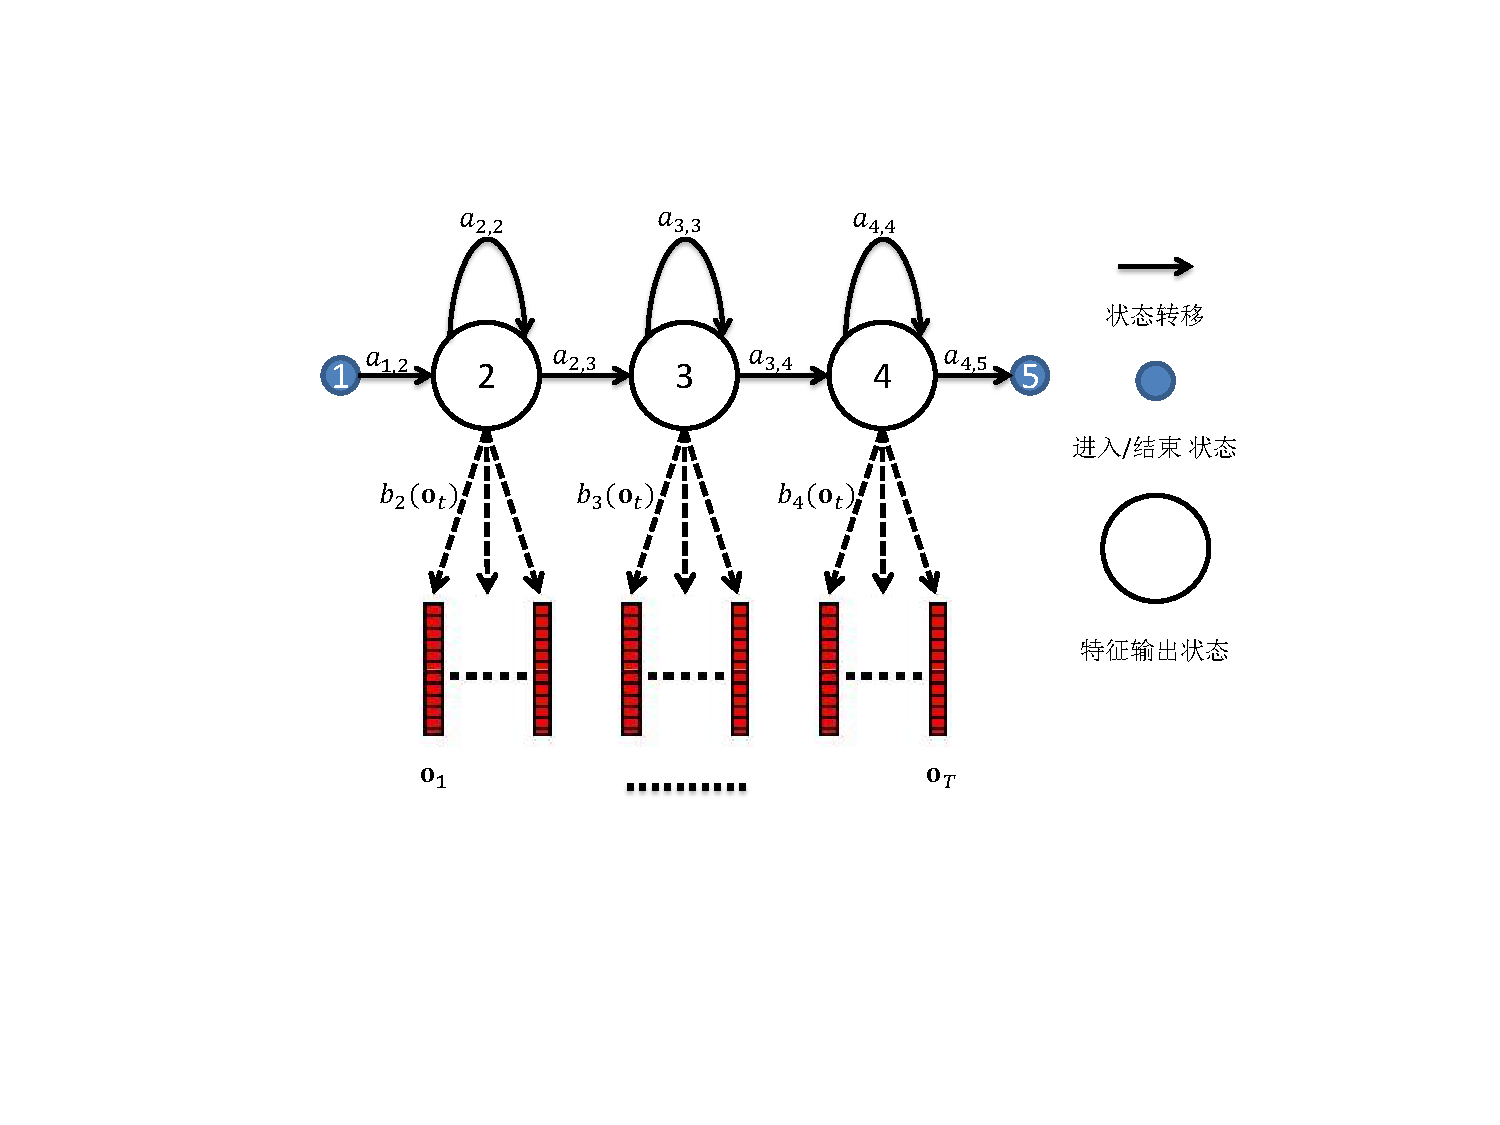
\includegraphics[trim = 3cm 5cm 4cm 3cm, clip=true, width=.7\textwidth]{figure/hmm.pdf}
    \bicaption[fig:hmm]{}{隐马尔可夫模型}{Fig}{Hidden Markov Model}
\end{figure}

令$\mathbf{O}=[\mathbf{o}_1, ..., \mathbf{o}_T]$为由一个声学单元生成的特征向量序列,其中$\mathbf{o}_t$是一个第$t$时刻的$D$维的语音特征向量,$T$是语音序列的总帧数。声学特征序列的生成过程如下面所示:
\begin{enumerate}
    \item 在第0时刻从状态1开始
    \item 在时刻$t$($0 \le t \le T-1$)。假设当前处于状态$i$,以概率$a_{i,i+1}$跳转到状态i+1或者以概率$a_{i,i}$停留在当前状态。
    \item 假设跳转完后处于状态$j$,若此时处在输出状态,则以$b_j(\mathbf{o}_t)$的概率输出声学向量$\mathbf{o}_t$。
    \item 重复2直至到达状态5
\end{enumerate}

这样我们可以利用一个状态序列来描述语音特征的输出过程$\mathbf{s}=[s_1, ..., s_T]$。而现实中我们只能观察到由状态输出语音特征序列,状态序列$\mathbf{s}$是隐藏的,这也是该模型被称为隐马尔可夫模型原因。一个隐马尔可夫模型通常包含如下参数:
\begin{itemize}
    \item $\pi$ 初始状态分布: \\
    令$s_t$表示在时刻t时所处状态,那么$\pi_i = P(s_0=i), \sum_{i=1}^N \pi_i = 1, \pi_i \ge 0$,其中$N$是总状态数。在拥有进入状态隐马尔可夫模型中,通常$\pi_1=1$。
    \item 状态转移概率矩阵$\mathbf{A}$: \\
    $a_{i,j}=P(s_{t+1}=j|s_t=i)$,在最常用5状态隐马尔可夫模型中,通常只有$a_{i,i}和a_{i,i+1}$不为0
    \item 状态输出概率分布$\mathbf{B}$: \\
    每个特征输出状态$i$都有一个概率分布来输出一帧声学特征,$b_i(\mathbf{o}_t)=p(\mathbf{o}_t|s_t=i)$
\end{itemize}

\subsubsection{混合高斯模型 (GMM)}
在传统的GMM-HMM中,状态输出概率$b_i(\mathbf{o}_t)$通常由一个混合高斯模型来建模。概率计算公式如下:
\begin{equation}
    b_i(\mathbf{o}_t)=\sum_{m=1}^{M_i}c^m_{i}\mathcal{N}(\mathbf{o}_t;\bm{\mu}^m_{i},\bm{\Sigma}^m_{i})
\end{equation}
其中$M_i$是属于第$i$个状态混合高斯模型含有的高斯成分个数,$c^m_{i}$是混合权重,满足$c^m_{i} \ge 0, \sum_{m=1}^{M_i} c^m_{i}=1$。$\mathcal{N}(\mathbf{o}_t;\bm{\mu}^m_{i},\bm{\Sigma}^m_{i})$是均值为$\bm{\mu}^m_{i}$,协方差矩阵为$\bm{\Sigma}^m_{i}$多变量高斯分布。
\begin{equation}
    \mathcal{N}(\mathbf{o};\bm{\mu},\bm{\Sigma})=(2\pi)^{-\frac{D}{2}}{|\bm{\Sigma}|}^{-\frac{1}{2}}e^{-\frac{1}{2}(\mathbf{o}-\bm{\mu})^{\top}\bm{\Sigma}^{-1}(\mathbf{o}-\bm{\mu})}
\end{equation}

\subsubsection{HMM的似然计算}
\label{sec:calc_like}
在定义好了HMM中分布之后,我们就可以计算隐马尔可夫模型的似然。似然计算目标是给定一个语音特征向量序列和一个隐马尔可夫模型,计算该模型生成给定的语音特征向量序列概率,即计算$p(\mathbf{O}|\mathbf{w},\mathcal{M})$,其中$\mathbf{O}$为观测到的语音特征向量序列,$\mathbf{w}$为对应文本标注,$\mathcal{M}=\{\pi, \mathbf{A}, \mathbf{B}\}$是所有模型参数。由于状态序列$\mathbf{s}$是隐藏,因而需要枚举所有可能的状态序列并求其期望,即:
\begin{eqnarray}
p(\mathbf{O}|\mathbf{w},\mathcal{M}) &=& \sum_{s}p(\mathbf{O},\mathbf{s}|\mathbf{w},\mathcal{M}) \\
&=& \sum_{\mathbf{s}} P(\mathbf{s}|\mathbf{w},\mathcal{M})p(\mathbf{O}|\mathbf{s},\mathcal{M}) \\
&=& \sum_{\mathbf{s}} a_{s_0, s_1}\prod_{t=1}^T a_{s_{t-1}, s_t}b_{s_t}(\mathbf{o}_t)
\end{eqnarray}
以上只考虑了单个隐马尔可夫模型似然计算。对于连续语音识别或利用子单词的声学单元,语音序列将对应一个模型序列。各个单词或者子单词单元之间准确时间边界是未知的,而解决方法则是扩展单隐马尔可夫模型,将若干个单独隐马尔可夫模型连接起来组成组合隐马尔可夫模型。

似然计算是利用和训练隐马尔可夫模型时需要考虑的最核心问题,直接枚举所有状态序列复杂度无疑是很高的。这一概率可以利用前向-后向算法快速计算,该算法也被称作鲍姆威尔士算法~\cite{baum1967inequality}(Baum-Welsh algorithm)。前向-后向算法通过利用动态规划思想,只需要$O(N^2T)$时间复杂度即可以计算出该概率,其中$N$是总状态数,$T$是总帧数。

定义前向概率$\alpha_i(t)$为到t时刻为止,且第t时刻所处状态为$i$,观测到特征序列$\left( \mathbf{o}_1, \dots, \mathbf{o}_t \right)$的概率。
\begin{equation}
\alpha_i(t)=p(\mathbf{o}_1, \dots, \mathbf{o}_t,s_t=i|\mathbf{w}, \mathcal{M})
\end{equation}
前向概率可以通过递归快速计算,对于$1<i<N, 0<t<=T$
\begin{equation}
\alpha_i(t)=(\sum_{j=1}^{N-1}\alpha_j(t-1)a_{j,i})b_i(\mathbf{o}_t)
\end{equation}
边界条件为:
\begin{eqnarray}
\alpha_i(t)=
\begin{cases}
1& i=1,t=0 \\
0& i \ne 1,t=0 \\
\sum_{j=2}^{N-1}\alpha_i(T)a_{j,N}& i=N, t=T+1
\end{cases}
\end{eqnarray}
对于常用于语音识别五状态HMM而言,因为转移只存在于相邻两个状态之间,所以时间复杂度减少为$O(NT)$。

同样我们可以定义后向概率$\beta_i(t)$为从第t时刻开始,且第t时刻所处状态为$i$的概率,观测到特征序列$\left( \mathbf{o}_{t+1}, \dots, \mathbf{o}_T \right)$概率。
\begin{equation}
\beta_i(t)=p(\mathbf{o}_{t+1},...,\mathbf{o}_T|s_t=i, \mathbf{w}, \mathcal{M})
\end{equation}
后向概率也可以通过递归快速计算,对于$1<i<N, 0<t<T$
\begin{equation}
\beta_i(t)=\sum_{j=1}^{N} a_{i,j} b_j(\mathbf{o}_{t+1}) \beta_j(t+1)
\end{equation}
边界条件为:
\begin{eqnarray}
\beta_i(t)=
\begin{cases}
a_{i,N} & t=T \\
\sum_{j=2}^{N-1} a_{1,j} b_j(\mathbf{o}_{1}) \beta_j(1) & i=1, t=0
\end{cases}
\end{eqnarray}
计算完前向概率和后向概率之后,可以很容易得到似然的公式为:
\begin{equation}
    p(\mathbf{O}|\mathbf{w}, \mathcal{M})=\alpha_N(T+1)=\beta_1(0)
\end{equation}

\subsubsection{最大似然估计}
训练GMM-HMM通常采用最大似然估计(Maximal Likelihood Estimation, MLE)准则。令$\mathcal{M}= \lbrace \{ a_{i,j}, 1 \le i,j \le N \}, \{ c^m, \bm{\mu}^m, \bm{\Sigma}^m, 1 \le m \le M \} \rbrace$为GMM-HMM中所有参数。其中$N,M$分别为总状态数和总高斯成分数。优化准则即为:
\begin{equation}
    \hat{\mathcal{M}}_{\text{MLE}} = \arg \max_{\mathcal{M}}\log p(\mathbf{O}|\mathbf{w}, \mathcal{M}) 
\end{equation}
由于存在隐藏变量,直接优化上述公式是很困难的,利用最大期望算法(Expectation-Maximization, EM)~\cite{dempster1977maximum}可对此进行优化。EM算法被广泛运用于含有隐变量统计学模型中,它基本思想是引入一个辅助函数作为log似然下界,通过不断迭代优化辅助函数来优化log似然函数。对于隐马尔可夫模型而言,辅助函数定义为:
\begin{eqnarray}
\mathcal{Q}_{\text{MLE}}(\mathcal{M}_{k+1};\hat{\mathcal{M}_{k}}) &=& \sum_{\mathbf{s}} P(\mathbf{s}|\mathbf{O},\mathbf{w}, \hat{\mathcal{M}}_k) \log p(\mathbf{O}, \mathbf{s}|\mathbf{w}, \mathcal{M}_{k+1}) \\
&=& \sum_{t,i} \gamma_i(t)\log b_i(\mathbf{o}_t) + \sum_{t,i,j}\xi_{ij}\log a_{i,j}
\end{eqnarray}
其中$\hat{\mathcal{M}}_k$是第$k$轮迭代计算出最优参数,
\begin{eqnarray}
\gamma_i(t)&=&P(s_t=i|\mathbf{O},\mathbf{w},\hat{\mathcal{M}}_k) \\
\xi_{ij}(t)&=&P(s_{t-1}=i,s_t=j|\mathbf{O},\mathbf{w},\hat{\mathcal{M}}_k)
\end{eqnarray}
EM算法是一个迭代的优化过程,其优化步骤如下:
\begin{enumerate}
    \item 初始化模型$\hat{\mathcal{M}}_0$
    \item 设当前迭代到第$k$轮,已经训练好模型参数$\hat{\mathcal{M}}_k$
    \item 利用$\hat{\mathcal{M}}_k$估计后验概率$\gamma_i(t)$, $\xi_{ij}(t)$。这两个概率可以由上一节提到的前向后向算法计算$\alpha,\beta$快速获得:
    \begin{eqnarray}
    \gamma_i(t)&=&\frac{\alpha_i(t)\beta_i(t)}{p(\mathbf{O}|\mathbf{w}, \hat{\mathcal{M}}_k)} \\
    \xi_{ij}(t)&=&\frac{\alpha_i(t-1)a_{i,j}b_j(\mathbf{o}_t)\beta_j(t)}{p(\mathbf{O}|\mathbf{w}, \hat{\mathcal{M}}_k)}
    \end{eqnarray}
    \item 利用最大似然估计$\hat{\mathcal{M}}_{k+1}$
    \begin{equation}
        \hat{\mathcal{M}}_{k+1} = \arg \max_{\mathcal{M}} \sum_{t,i} \gamma_i(t)\log b_i(\mathbf{o}_t) + \sum_{t,i,j}\xi_{ij}\log a_{i,j}
    \end{equation}
    \item 转移概率更新为:
    \begin{equation}
        \hat{a}_{i,j}=\frac{\sum_{t=1}^T \xi_{i,j}(t)}{\sum_{t=0}^{T+1} \gamma_i(t)}
    \end{equation}
    \item 当利用GMM作为状态输出概率时,高斯成分的索引可以被视为一个特殊隐子状态,转移概率是各成分的权重乘以状态转移概率。因此可以求得各个高斯成分后验占用率:
    \begin{equation}
        \gamma^m_j(t)=\frac{\sum_{i=2}^{N-1}\alpha_i(t-1)a_{i,j}c^m_{j}\mathcal{N}(\mathbf{o}; \bm{\mu}^m_j, \bm{\Sigma}^m_j)\beta_j(t)}{p(\mathbf{O}|\mathbf{w}, \hat{\mathcal{M}}_k)}   
    \end{equation}
    这里$\gamma^m_j(t)$表示状态$j$的第$m$个高斯成分在第$t$包含后验占有量。
    \item GMM的参数更新为:
    \begin{eqnarray}
        \hat{c}^m_j &=& \frac{\sum_{t=1}^T \gamma^m_j(t)}{\sum_{m,t} \gamma^m_j(t)} \\
        \hat{\bm{\mu}}^m_j &=& \frac{\sum_{t=1}^T \gamma^m_j(t) \mathbf{o}_t}{\sum_{t=1}^T \gamma^m_j(t)} \\
        \hat{\bm{\Sigma}}^m_j &=& {\tt diag} \left( \frac{\sum_{t=1}^T \gamma^m_j(t) (\mathbf{o}_t-\hat{\bm{\mu}}^m_j)(\mathbf{o}_t-\hat{\bm{\mu}}^m_j)^{\top}}{\sum_{t=1}^T \gamma^m_j(t)} \right)
    \end{eqnarray}
    在公式中,我们只估计了协方差矩阵对角元素。由于在大词汇连续语音识别任务中通常需要利用大量高斯成分,在此基础上若利用满秩矩阵将对计算和存储资源需求巨大,因而对于每个高斯成分,通常只利用对角矩阵。
    \item 重复2直到收敛
\end{enumerate}
虽然利用最大似然估计GMM-HMM已获得了巨大成功,然而只有在拥有充足数据量和正确的模型假设前提下它才是合适优化准则。现实中,由于在HMM模型中存在马尔可夫和条件独立性两个假设,并不符合真正语音生成过程,因此利用最大似然估计来最优化HMM将无法估计出最合适的参数。其中一个解决方案就是利用序列鉴别性训练准则~\cite{bahl1986maximum,schluter2001comparison,chou1993minimum,goel2000minimum,juang1997minimum,povey2005discriminative,povey2001improved}

\subsubsection{序列鉴别性训练}
在基于最大似然估计中,优化目标是给定标注生成语音特征向量序列的似然。鉴别性训练与之不同处在于:鉴别性训练优化目标为最大化给定语音特征向量序列所对应文本标注的后验概率,即最大化$P(\mathbf{w}_{\text{ref}}|\mathbf{O})$。这样相当于直接将语音识别评判准则引入优化目标之中。目前最先进的语音识别系统中都利用了序列鉴别性准则。这章将简单地介绍其中两种:最大互信息(Maximum Mutual Information, MMI)和最小贝叶斯风险(Minimum Bayes' Risk, MBR)
\begin{itemize}
    \item 最大互信息 \\
    最大互信息准则在后验概率$P(\mathbf{w}_{\text{ref}}|\mathbf{O})$基础上增加一个经验缩放$\kappa$\footnote{它的作用是为了使不太可能假设对准则有所贡献,并使准则更加平滑可区分,通常等于识别中利用的语言模型缩放系数倒数},它的优化目标如下:
    \begin{equation}
        \mathcal{F}_{\text{MMI}}(\mathcal{M})=\frac{p^{\kappa}(\mathbf{O}|\mathbf{w}_{\text{ref}},\mathcal{M})P(\mathbf{w}_{\text{ref}})}{\sum_{\mathbf{w}}p^{\kappa}(\mathbf{O}|\mathbf{w},\mathcal{M})P(\mathbf{w})}
    \end{equation}
    这里$\mathbf{w}_{\text{ref}}$是语音特征向量序列对应标注,$\mathbf{w}$是所有可能的标注序列,包括正确标注和错误标注。虽然理论上$\mathbf{w}$应该包括所有可能词序列,实际上通常只考虑最具有混淆性标注。它通常由在训练数据上解码生成N-Best列表或者词图构成。
    \item 最小贝叶斯风险 \\
    最小贝叶斯风险准则目标在最小化期望损失,即
    \begin{equation}
        \mathcal{F}_{\text{MBR}}(\mathcal{M})=\sum_{\mathbf{w}}P(\mathbf{w}|\mathbf{O};\mathcal{M})L(\mathbf{w},\mathbf{w}_{\text{ref}})
    \end{equation}
    这里$L(\mathbf{w},\mathbf{w}_{\text{ref}})$是标注与候选的标注之间损失函数,通常包含句子层,单词层和音素层。
    \begin{itemize}
        \item 句子层:这一准则希望最小化句子层的错误
        \begin{eqnarray}
            L(\mathbf{w},\mathbf{w}_{\text{ref}})=
            \begin{cases}
                1& \mathbf{w} \ne \mathbf{w}_{\text{ref}} \\
                0& \mathbf{w} = \mathbf{w}_{\text{ref}}
            \end{cases}
        \end{eqnarray}
        \item 损失函数也可以定义在词层面(最小词错误)和音素层面(最小音素错误)。比如在最小词错误中,$L(\mathbf{w},\mathbf{w}_{\text{ref}})$为两个词序列之间编辑距离,即词错误数。最小音素错误在最先进语音识别系统中利用非常广泛~\cite{povey2005discriminative}
    \end{itemize}
\end{itemize}

\subsubsection{声学单元和参数绑定}
当进行小词汇语音识别时,如识别数字时通常可以用隐马尔可夫模型直接建模独立的单词。然而当词汇数量从中等词汇上涨到大词汇(>10000)时,利用隐马尔可夫模型来建模每一个词汇变成了不可能事情。一个广泛利用的解决该问题方法为建模子词单元。

音素是一个被广泛利用的子词单元,它是语音中最小声学元素。利用音素的好处是存在将每个词转换为音素标准,这样每个词能很容易的被分解成各个音素。在音素上建模的模型被称作音素模型,音素数目一般远远小于待识别词的个数。在当前最先进大词汇连续语音识别系统里,通常利用46个音素。

利用音素能更容易的获得足够数据以训练出更具有鲁棒性的模型参数。需要注意是当利用音素来建模时,需要提供一个字典用于将单词序列映射成子词单元序列,然后才能在子词单元的层面进行识别和运算。在识别最后,还需要将子词单元序列转换回单词序列。

目前有两种被广泛利用音素集合。一种是单音素,也称为上下文无关音素;另一种则是上下文相关音素。由于协同发音现象的影响,当前音素发音和前一个、后一个音素之间具有很强的相关性,所以在许多识别任务里,仅仅利用单音素效果不是很好。为了建模协同发音现象,目前最先进语音识别系统利用的是上下文相关音素,其中三音速利用最为广泛,它将当前音素的前一个和后一个音素同时建模。

比如,以one来说,它对应三音素序列即扩展为one=\{sil−w−ah, w-ah-n, ah-n-sil\}。虽然利用更多的上下文信息可以建立更复杂的音素模型,如五音素~\cite{hain2005automatic}(quin-phones),但三音素依然是目前利用最广泛音素模型。根据是否考虑单词间的边界,三音素模型可以继续细分为跨单词三音素和单词内三音素。跨单词三音素允许三音素的扩展跨越单词:在两个单词边界,当前音素的前一个和后一个音素分别是上一个单词的最后一个音素和下一个单词第一个音素。词内三音素则相反,音素只能在单词的内部进行扩展。因此,在每个单词开头和结尾,是一个双音素。跨单词三音素在大规模词汇连续语音识别系统里效果更好~\cite{woodland1994large}。

利用三音素后,声学单元个数将变得巨大。当利用46个单音素时,所有可能的三音素个数达到了$46^3=97336$,这一数字甚至超过了词表大小,不可能有充足数据能训练如此大的模型。目前一个通用解决该问题的方法是利用参数共享~\cite{young1993use, young1994tree}。它基本思想是将一些参数绑定在一起。参数共享可以存在于各个层面,包括音素,状态,高斯等。由于利用最广泛的是在状态共享层面,因而也被称为状态聚类。在利用状态聚类时,来自同一组的状态将共享状态输出分布,每一个实际状态输出分布被称为一个语素(senone),如图\ref{fig:state-tying}所示。
\begin{figure}[!htp]
  \centering
    \captionstyle{\centering}
    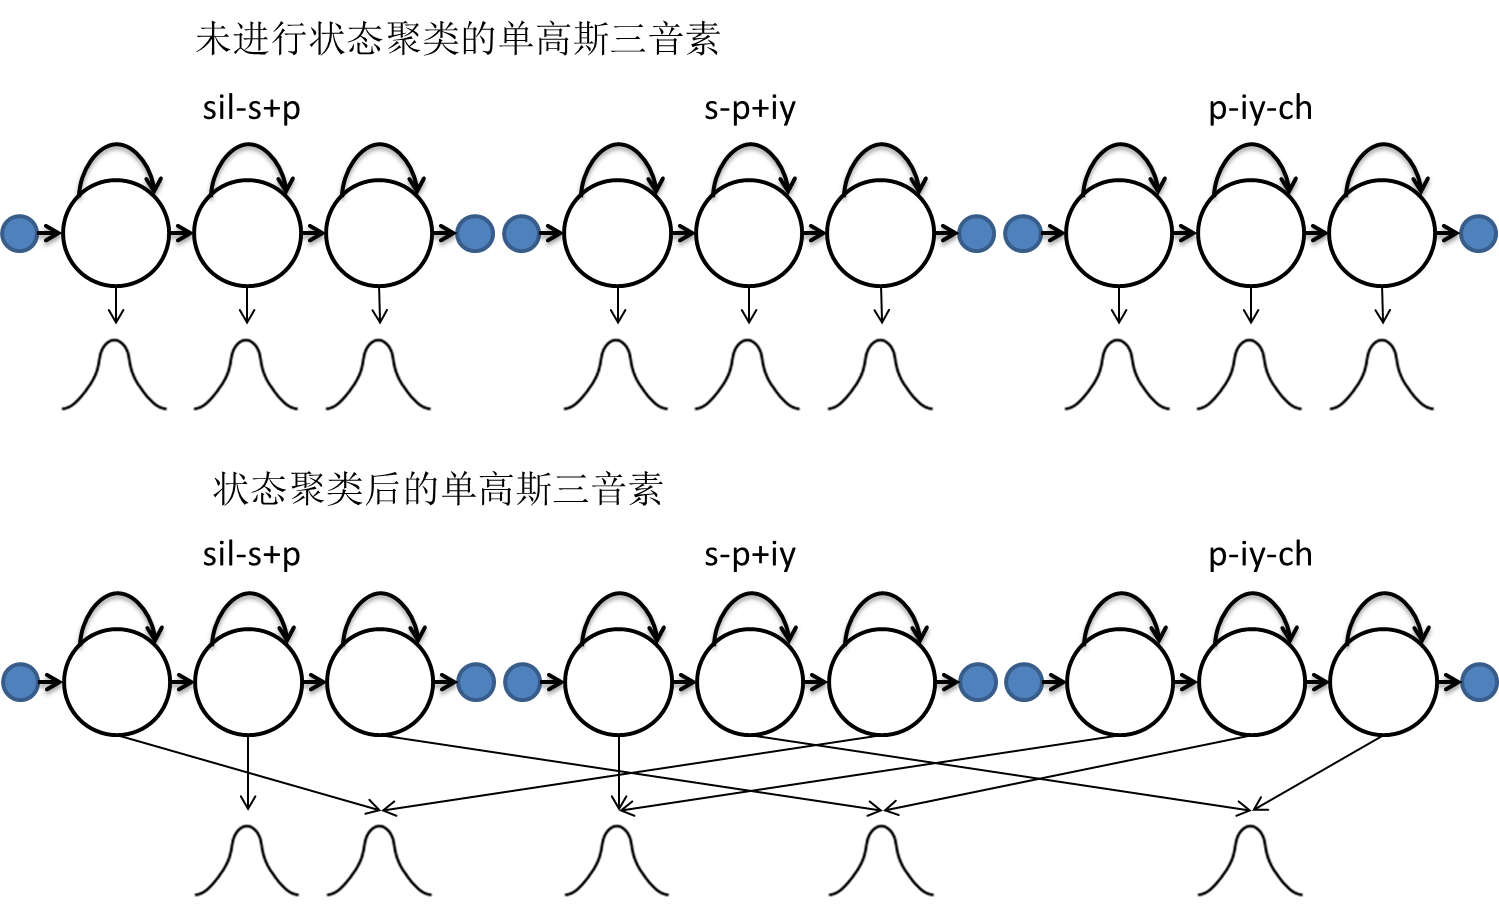
\includegraphics[width=.8\textwidth]{figure/state.png}
    \bicaption[fig:state-tying]{}{单高斯三音素的状态聚类}{Fig}{State clustering for single gaussian triphones}
\end{figure}

目前利用最广泛的聚类方法是基于数据驱动自底向上聚类。对训练集中存在的每一对语素之间计算一个距离,距离在某个阈值以内的语素将会被聚集在一起。数据驱动的主要问题在于当没有足够多训练数据时,这一方法将不再可靠,更严重的是,训练数据中不存在信息将无法被捕捉到。

另外一个更好的方法是利用音标决策树的方法来进行聚类。音标决策树是一棵包含了一系列关于每个音素左右上下文问题的二叉树,因为问题答案只有对和错。聚类自上而下开始,所有的状态都从根节点出发,通过回答上下文问题来分割左右儿子。直至处于当前节点的训练数据状态数目小于一个阈值,分割过程停止,此时叶子节点即为一个语素。决策树中的关键难题在于提问的顺序,目前最常用方法是在每次分裂时挑选能在分裂后似然增加的最大的那个问题。虽然这样决策树可能陷入局部最优,但它确实有效处理了对于不可见的三音素分类问题。

\subsection{语言模型}
\label{sec:lm}
语音模型建模的是候选标注的先验概率,假设候选标注含有$K$个单词,$\mathbf{w}=\{w_1, \dots, w_K\}$。通过条件概率公式,语音模型概率可以扩展为若干条件概率连乘:
\begin{equation}
    \label{eq:lm}
    P(\mathbf{w})=\prod_{k=1}^{K}P(w_k|w_{k-1}, ..., w_1)
\end{equation}
这里$w_k$是序列中的第$k$个单词。利用公式\ref{eq:lm}来计算先验概率需要记录整个句子的历史,然而在大词汇语音识别任务中,由于词表大小往往能达到10000词以上,所有可能的历史数据太过庞大,因此很难对每个可能的词序列都进行鲁棒估计。一种解决方案是限制历史的长度,N元组(n-gram)语音模型即利用了这一策略,它也是目前语音识别中最广泛利用的统计语言模型。它所作出假设是只需要最多利用N个单词作为历史就足够计算概率:
\begin{equation}
    P(w_k|w_{k-1}, ..., w_1) \approx P(w_k|w_{k-1}, ..., w_{k-N+1})
\end{equation}
这里$N$是预先定义的历史窗口大小,语音识别中通常利用$N=3$,也被称为三元语言模型。语言模型通常利用最大似然的准则进行训练,它的更新公式如下:
\begin{equation}
    P(w_k|w_{k-1}, ..., w_{k-N+1})=\frac{f(w_k,w_{k-1},...,w_{k-N+1})}{\sum_wf(w,w_{k-1},...,w_{k-N+1})}
\end{equation}
这里$f(w,w_{k-1},...,w_{k-N+1})$表示这$N$个词按顺序出现在训练数据中的个数。因为采用是最大似然估计,所以每个N-元序列得拥有充足的样本才能得到最鲁棒的估计。然而,即使$N$非常小,这一条件在大词汇连续语音识别任务中依然很难达成。所以,过去研究提出了若干平滑的方法来获得鲁棒的估计。
\begin{itemize}
    \item 降权(Discounting) \\
    降权方法用于解决训练集中未观测到N元组概率无定义的问题,它的主要思想是将被观测到的N元组概率乘上一个降权系数,将剩下的部分平均分配给未观测到N元组。最常用的降权方法有Good-Turing法~\cite{good1953population,katz1987estimation},Witten-Bell法~\cite{witten1991zero}和绝对降权法~\cite{ney1995estimation}
    \item 回溯法(Backing-off) \\
    回溯法利用训练数据中观测到的具有较短历史信息的词序列的组合概率来近似那些没有出现过、由较长历史信息组成词序列组合。
    \item 多模型插值(Interpolation) \\
    当一个N元语言模型不是很鲁棒时,可以通过和更低阶的语言模型进行插值以获得更平滑模型,比如在语音识别中通常会将单元,二元和三元语言模型进行插值来构建一个更鲁棒语言模型。插值的权重通常在一个校验集上调节得到。同样,我们也可以用同样的方法对由不同语料训练出N元语言模型进行插值。
\end{itemize}
语言模型训练和评价指标通常是困惑度(Perplexity, PPL),它定义是词序列生成概率的几何平均倒数:
\begin{equation}
    \text{PPL}=2^{-\frac{1}{K}\log(P(\mathbf{w}))}
\end{equation}
其中$K$是词序列包含的总词数,拥有更低PPL语言模型具有更低的不确定度和混淆度,通常也能潜在的降低语音识别词错误率。当然,这一关系并非一直成立,因而在语音识别中最终还是以词错误率来判断语言模型的好坏。

\subsection{解码及搜索}
\label{sec:decode}
如公式\ref{eq:asr}所示,解码的过程是在给定声学模型和语言模型之后寻找拥有最大概率路径。
\begin{eqnarray}
\mathbf{w}^* &=& \arg \max_{\mathbf{w} \in \mathcal{H}}p(\mathbf{O}|\mathbf{w})P(\mathbf{w}) \\
&=& \arg \max_{\mathbf{w} \in \mathcal{H}} \sum_{\mathbf{s}} P(\mathbf{s}|\mathbf{w})p(\mathbf{O}|\mathbf{s})P(\mathbf{w})
\end{eqnarray}
这里$\mathbf{s}$是所有可能的状态序列,$P(\mathbf{w})$通过语言模型计算,$P(\mathbf{s}|\mathbf{w})p(\mathbf{O}|\mathbf{s})$通过声学模型计算。正如我们在章节\ref{sec:calc_like}中讨论过的,这一似然可以通过前向后向算法进行计算。然而,因为候选词序列可能性过于庞大,无法通过对每个候选进行前向后向算法来计算似然。因此,实际中通常利用最大概率的状态路径来近似整个概率,即:
\begin{equation}
\label{eq:decode}
\mathbf{w}^* = \arg \max_{\mathbf{w} \in \mathcal{H}} \max_{\mathbf{s}} P(\mathbf{s}|\mathbf{w})p(\mathbf{O}|\mathbf{s})P(\mathbf{w})
\end{equation}
这样我们可以通过利用动态规划(Dynamic Programming, DP)的方法计算出拥有最大概率状态序列,然后以此推理出词序列,这一算法被称为Viterbi算法~\cite{viterbi1967error}。另$\phi_i(t)$表示在时刻$t$且输出了部分从$\mathbf{o}_1$至$\mathbf{o}_t$声学特征后停留在状态$i$的最大概率。它可以利用递归来计算:
\begin{equation}
    \phi_i(t)=\max_j\{\phi_j(t-1)a_{j,i}\}b_i(\mathbf{o}_t)
\end{equation}
这里$a_{i,j}$是状态转移概率,$b_i(\mathbf{o}_t)$是状态输出概率。最终:
\begin{equation}
    p(\mathbf{O}|\mathbf{w}) \approx \phi_{N}(T+1) = \max_i\{\phi_i(T)a_{i,N}\}
\end{equation}
Viterbi算法可以很容易扩展到连续语音识别,一种扩展后的Viterbi算法也被称为令牌传递(Token Passing)算法~\cite{young2002htk}。在这一算法中,每一个状态将不仅仅保留一个最优路径,而是保存若干个令牌。每一个令牌记录着某个候选词序列在第$t$时刻到达状态$i$的最优路径。在到达一个词边界时,语言模型的分数会直接加上。在整个观测序列结束时,拥有最大概率的令牌将被提取出来回溯其整个HMM序列。

即使利用了令牌传递算法,在大词汇连续语音识别中,传播所有令牌搜索代价依然十分庞大。为了减少计算代价,通常会利用基于集束搜索(beam search)剪枝方法。在这一方法中,所有$\phi_i(t)$低于$i$中最大概率减去一个阈值的令牌都会被移除,这一阈值也被称为集束(beam)宽度,剪枝也可以在加完语言模型之后进行。虽然beam搜索方法可以显著减少计算量,但是有可能在早期阶段利用了过窄的beam宽度而剪去了真正最优路径导致识别错误。所以,beam宽度设置需要在减少计算量和提升识别准确率之间进行均衡。

语言分数和声学分数之间动态范围的区别也是需要考虑问题,通常会分别对声学分数和语言分数进行缩放。另外需对插入错误添加额外惩罚,从而均衡词错误率中的插入和删除错误比例,因而最终语音识别中利用的准则是:
\begin{equation}
\mathbf{w}^* = \arg \max_{\mathbf{w} \in \mathcal{H}} \{\log p(\mathbf{O}|\mathbf{w}) + \alpha \log P(\mathbf{w}) + \beta L_{\mathbf{w}}\}
\end{equation}
这里$\alpha$是语言模型分数缩放系数,$\beta$是插入错误惩罚系数,$L_{\mathbf{w}}$是词序列长度。
通常会选择最大概率路径作为识别结果,也可以输出若干候选结果然后用更强的语言模型来重新评价(比如利用神经网络语言模型)。这一候选结果一般利用N-best列表~\cite{schwartz1990n}或者利用能包含更多信息词图(Word Graph/Word Lattice)~\cite{ortmanns1997word}。近些年来,基于加权有限状态机(Weighted Finite-State Transducer, WFST)~\cite{mohri2002weighted}的解码器被越来越多人采用,它的优点是可以将语言模型提前融合成一个网络,从而在解码时加快解码速度。




\section{大词汇连续语音识别中解码搜索技术}
\label{chap:intro-lvcsr}

语音识别既是一个模式识别问题,也包含相应的推理问题。前一个问题对各种语音、语言现象进行数学表示和描述,在基于统计学习的模式识别框架下进行建模,这决定了语音识别系统可达到识别精度的上限。而后一个问题在给定模型情况下,研究如何将输入语音和模型相匹配,推理得到最优识别结果,这决定了识别速度和实际可达的识别精度。
%
在语音识别的推理阶段,解码器功能是对声学模型计算出的声学特征概率和语言模型计算出的语言概率进行组合来得到最大概率的词序列。
%
在语音识别推理阶段,解码器是语音识别系统的核心和灵魂,所有信息都汇集于此。它将不同来源、 不同层次、 不同性质的知识和信息关联在一起,使它们互相之间取长补短, 从而得到正确的语音识别结果。因此,如何将各种性质相异信息有机融合是解码网络和解码算法设计中必须认真研究和解决的问题。
从解码器的作用来看,它既是语音识别研究中验证各种理论、模型、算法
正确性的基本实验平台,也是构建实用系统的基础。因此,在解码器设计中也
需要兼顾研究的方便与工程实际应用。

\subsection{解码器的技术流派}
\label{chap:intro-lvcsr-decmethod}

根据前面章节讨论,一个完整的语音识别系统包含了自底向上的五层映射关系:
语音观测到 HMM 状态、 HMM 状态到上下文相关音素、上下文相关音素到音素、
音素到词、词到句子。
具体来说公式~\ref{eq:decode}可以进一步展开如下:
\begin{equation}
 \begin{split}
\mathbf{w}^* = \arg \max_{\mathbf{w} \in \mathcal{H}} \max_{\mathbf{s}} P(\mathbf{s}|\mathbf{w})p(\mathbf{O}|\mathbf{s})P(\mathbf{w}) \\
= \arg \max_{\mathbf{w}} \sum_{\mathbf{l}} \sum_{\mathbf{c}} \sum_{\mathbf{s}}
p(\mathbf{O}|\mathbf{s}) \cdot
P(\mathbf{s}|\mathbf{c})\cdot P(\mathbf{c}|\mathbf{l})\cdot P(\mathbf{l}|\mathbf{w}) \cdot 
P(\mathbf{w})
 \end{split}
\end{equation}
其中展开后式子每一项分别对应上述的五层映射关系。
语音观测无法在识别之前得知,因此语音观测到 HMM 状
态的映射需要在解码过程中动态建立,对应声学分数也需要实时计算。
对于 HMM 状态到上下文相关音素、上下文相关音素到音素、音素到词这三层映
射关系,一旦发音字典、声学模型确定便不再改变。出于对解码效率的追求,人
们通常把它们静态地编译到解码网络中去。对于没有任何约束的大词汇连续语音识别任务而言,
词可以以任意方式组织成句, 故而从原理上讲, 词、 句间映射关系只能在解码
过程中动态建立。 但是由于表征词与词之间关联度(概率)的 N 元文法模型在解
码前便已存在且是一个有限集合, 所以在实际中, 语言模型分数计算却可
以用不同的方式实现。 在语音识别领域,通常根据解码器中语言模型的表示、 语
言模型状态获取以及语言模型分数计算方法的不同把解码器分为两大流派:
\begin{itemize}
\item 动态网络解码器: 在动态网络解码器中,解码网络仅包含发音字典和声学
模型,不含有语言模型任何信息。 语言模型状态在解码过程中随着词与词相连
成句而动态地生成、语言模型分数通过查表的方式动态获取。这类解码器的典型
代表是基于发音前缀树(Pronunciation Prefix Tree, PPT)~\cite{woodland1994large}网络解码器。
\item 静态网络解码器: 在静态网络解码器中,解码网络不仅包含发音字典和声
学模型,也包含完整的语言模型。 语言模型状态以及状态转移以有限状态机的形
式合成进解码网络中去, 语言模型分数则作为状态转移概率存储于边上。解码时,
仅需逐边积累整条路径状态转移概率便可获得语言模型分数。这类解码器的典
型代表是基于加权有限状态转换器(WFST)~\cite{mohri2002weighted}的解码器。
\end{itemize}

静态网络解码器作为一种以空间换时间策略,通过精心的优化,一般可以
获得更快的识别速度, 但是其缺点也是显而易见,即:构建的解码网络规模过
大,尤其是在采用高阶语言模型和声学模型情况下,由于内存大小限制,要
将所有的知识源都编译进解码网络中往往是不可行。因此,近年来基于动态解
码网络传统语音识别方法又逐渐受研究人员青睐~\cite{soltau2009dynamic,rybach2011comparative}, 能够几乎不受任何约束
地利用高阶语言模型和声学模型以便获得更优的识别精度, 应用面更广, 这是动
态网络解码器最为诱人之处。然而动态网络解码器的设计和束搜索剪枝方法更为
复杂,需要调整参数和门限更多,挑战性更大。 

除了从解码网络的结构上进行分类,还可以根据搜索最优路径不同方式,
将解码器分为时间异步搜索解码器和时间同步搜索解码器:

\begin{itemize}
\item 时间异步搜索解码器: 在较老的解码器,例如: IBM ViaVoice 中, 采用深
度优先方式在解码网络中搜索最优词序列, 是一种时间异步搜索。由于这类解码
器在解码过程中需要用到若干后进先出的缓冲区(即:堆栈)来保存扩展得到
词识别假设,所以也常常被称为堆栈解码器(Stack decoder)~\cite{paul1992efficient}。 
与时间同步搜索相比,其好处在于:通过选取适当启发式函数(Heuristic function),可以将搜
索局限于最优路径附近,提高搜索效率。 但这也造成了它的主要缺陷: 1) 启发式
函数要综合声学和语言两方面分数,有时还需要“将来”路径的信息, 因此非
常难以获得; 2)由于是时间异步搜索,所以搜索过程中产生路径长度各不相同,
使得剪枝难于实现。因此,目前堆栈解码已很少用于直接对语音观测进行解码,
而是更多地作为一种后处理手段, 用于从词图中生成 N-Best 结果。
\item 时间同步搜索解码器:时间同步搜索是目前解码器设计与实现中主流方
法,又称帧同步搜索。它采用广度优先方式从解码网络中找出与输入特征序列最
匹配的状态序列,从而得到相应的最优音素序列和词序列。这一类解码器通常采
用 Viterbi 算法或是令牌传递(Token passing)算法~\cite{woodland1994large}实现。 
\end{itemize}

解码器不仅算法复杂,并且实现起来需要较高工程化能力和技巧, 在开发
完成后也往往需要不小人力和时间才能够调优, 因此各个研究机构与商业公司
都对自己解码器的实现细节讳莫如深。 尽管如此,目前世界上还是存在一些以学
术研究为目的开源解码器可以作为研究的基础, 表
列出了其中较为知名。这些解码器的网络结构和解码算法各异,但由于是以学术研究为目的,因此速度
优化方面大部分较差。


\begin{table}[thbp!]
  \caption{\label{tab:perf-compare} {\it  知名开源解码器 } }
  \centerline{
    \begin{tabular}{c c  c c}
      \toprule
      解码器 &  研发机构 & 网络结构 & 搜索算法 \\
      \midrule
      HDecode & 英国剑桥大学 & 动态,发音前缀树 & 单遍, 令牌传递 \\
        Sphinx &美国卡内基梅隆大学 &动态,发音前缀树 &单遍, 令牌传递 \\
        RASR &德国亚琛工业大学& 动态, 发音前缀树 &单遍, Viterbi \\
        Juilus & 日本京都大学 & 动态, 发音前缀树 & 两遍, 前后向搜索。\\
        Juicer & 瑞士IDIAP & 静态, WFST & 单遍,令牌传递 \\
        Kaldi & 美国约翰霍普金斯大学 & 静态, WFST & 两遍,令牌传递     \\
\bottomrule
    \end{tabular}
  }
\end{table}

多遍搜索与单遍搜索(1-pass)相比各有优劣,在实际中也都有应用。多遍搜
索的拥护者认为: 通过第一遍粗搜索可以大大缩小解码空间, 使得在后续解码过
程中利用更加精细语言模型和声学模型成为可能,避免了单遍解码器中的时间、
空间约束问题。单遍搜索的拥护者认为多遍解码有三个主要问题: 1) 由于第二遍
解码必须等待第一遍解码完成,所以多遍搜索很难应用于实时解码。 2) 每一遍解
码都会引入不可恢复剪枝错误,这些错误不论在后续解码中采用何种模型都无
法弥补。要解决这一问题还是得在单遍搜索算法上下功夫,与其这样,还不如直
接做好单遍解码器。 3) 多遍解码器的每一遍解码采用的特征、声学模型、语言模
型、搜索算法都不尽相同。

\subsection{结构和主要模块}
\label{chap:intro-lvcsr-decmodule}

\subsubsection{解码器框架}

图~\ref{fig:dec_arch}给出了典型解码器结构。不论是哪种类型解码器通常都包含网络生
成、分数计算、搜索、剪技与路径管理这五部分,它们的功能逐一介绍如下。

\begin{figure}[!htp]
  \centering
    \captionstyle{\centering}
    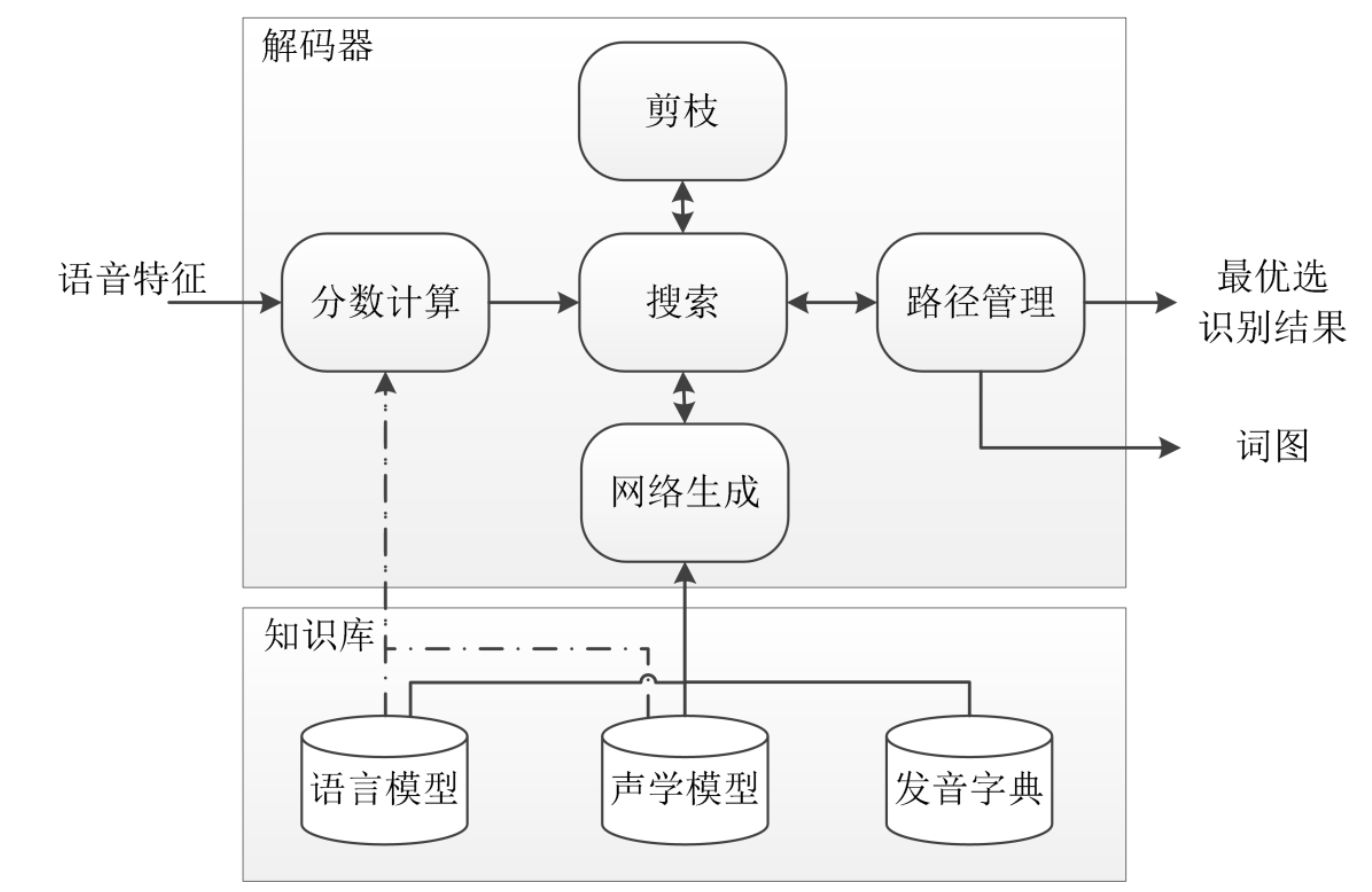
\includegraphics[clip=true, width=.9\textwidth]{figure/dec_arch.png}
    \bicaption[fig:dec_arch]{}{通用解码器架构}{Fig}{General Architecture of ASR Decoder}
\end{figure}


\subsubsection{网络生成}

网络生成模块主要负责将构建解码搜索空间。搜索空间,又称解码网络, 一般以音素 HMM 或 HMM 状态连缀而成,由语言模型、发音字典、声学模型和其
他相关知识源编译而来。
大词汇连续语音识别系统解码网络是由各个知识源构成一个搜索空
间,一般来讲可以分为动态构建的解码网络和静态网络。基于动态网络的解码
器,以前缀树发音词典作为搜索网络,语言模型则通过动态查询方式把得
分引入解码过程之中,然后利用重入字典树或者字典树拷贝的方式对整个解
码网络进行搜索~\cite{young2002htk}。动态网络解码器优势在于,由于字典和语言模型是分
离,其占用内存较少,这个特点在以往移动网络技术和硬件技术不发达的时
期,尤其是在嵌入式设备上内置解码器的时代占有绝对优势,这是由嵌入设备
硬件条件决定的。但是动态网络的缺点是它时间复杂度较高、解码速度较
慢,这也使其越来越难以满足当前海量语音识别需求。随着移动互联网
和嵌入式设备的普及以及云技术发展,语音识别应用发展为在嵌入式设备
上仅仅保留简单的前端,而识别系统保留在服务器云端。这时基于加权有限状
态机的静态网络解码器快速优势就体现出来了,更短的识别时间能让服务器
在单位时间内接受更多识别任务,因此静态编译的解码网络更适合用于海量
的语音识别任务。

在 LVCSR 任务中,解码网络通常非常庞大,因此网络生
成过程中需采用多种手段对网络结构进行优化,在不改变网络功能前提下,尽
可能地减少网络中节点和边的数目。 解码网络是解码器基础,决定了解码器
其他部分应当采用何种方法实现。在静态网络解码器中,解码网络不仅包含发音字典和声
学模型,也包含完整的语言模型。 语言模型状态以及状态转移以有限状态机形
式合成进解码网络中去, 语言模型分数则作为状态转移概率存储于边上。解码时,
仅需逐边积累整条路径状态转移概率便可获得语言模型分数。这类解码器的典
型代表是基于加权有限状态转换器(WFST~\cite{mohri2002weighted}的解码器。

加权有限状态机最开始是由AT\&T实验室Mohri和Riley等人在1997年引
入语音识别领域的。并且在理论上发展了确定化、最小化等一系列网络优化算
法,为语音识别的应用打好了理论基础。语音识别各模型组件分别用如下方式进行WFST构建:

\begin{itemize}
\item N元语言模型在WFST中被表示为G。从N元语言模型的含义可知,它提供的是当前词对于词历史
概率。语言模型需要有信息记录其至多N个词的历史。但是,WFST应用在语音
识别时是不允许输入输出带有串的(即输入输出都是其符号集单个元素)。
因此不能用G构造过程的输入输出上表示其历史,而应选用在状态上记录历史。
另外一个问题是N元语言模型的回退(Back-off),当语言模型训练语料
未出现某一个N元词组的时候,就会以一个回退的(N-1)元模型概率乘以一个
系数来替换。这部分表示为一个带有权重空输入的状态跳转边。

\item 字典在WFST中被表示为L。
字典其实是对发音规则的一种表示,最简单方法就是在开始状态和结尾
状态之间列出每个词的发音。同时,由于在和语言模型合成的时候,词与词是
相连,不能够到达终止状态就完结了,需要用一个空边从终止状态连接到开
始状态形成一个闭环。
针对字典的同发音问题,Mohri在文献~\cite{mohri2002weighted}中提出对于不同词的同发音发音
序列加入一组辅助符号,这样对于同发音词,其环路的输入
符号就不再相同,可以确保字典的可确定化。

\item 上下文相关声学模在WFST中被表示为C。
一个上下文相关triphone模型一般表示为a-b+c,其中b是中心音素,
a和c为其前后上下文音素~\cite{seide2011conversational}。用WFST表示triphone模型实际上是把三音素
和单个的音素进行对应,其输出就和发音字典的输入相互对应,由此可以进行进一步合成。

\item 隐马尔可夫模型在WFST中被表示为H。
隐马尔可夫模型天然具有多个状态跳转特性,因此可以直接将其构建为多个WFST状态。隐马尔科夫模型的转移概率被转化为WFST的权重。而WFST输入是隐马尔科夫模型的状态编号,输出是该隐马尔科夫模型所表示的triphone建模单元。
\end{itemize}

当各个知识源WFST组件被构建完毕以后,可以利用WFST合成和优化算法将各组件最后进行合并。如下:
\begin{equation}
HCLG = min(det(H \circ min(det(C \circ min(det(L \circ G))))))
\end{equation}

最终生成的WFST包含了所有的知识源,后文所讨论维特比搜索就在它上面进行。

\subsubsection{分数计算}

分数计算模块计算输入特征序列声学和语言分数, 提供给搜索模块利用。
应当计算何种分数与解码网络结构和搜索算法有关。例如,在静态网络解码器中,
语言模型分数已编译于解码网络之中,所以只需要计算声学分数即可;而对于动
态网络解码器, 除声学分数外, 还需要计算语言模型分数。 在分数计算方面研
究主要集中于如何实现分数的快速计算, 对于声学分数通常从如下三个方面进行:

\begin{itemize}
\item 硬件加速。利用 CPU 矢量计算器~\cite{kanthak2000using}
或通用图形处理器(Graphics
Processing Unit, GPU)~\cite{chong2009fully}
加速分数计算。这类方法通常不会带来计算误
差(与硬件实现相关),所以对识别精度没有影响。
\item 模型简化。采用复杂度更小、参数更少的模型,或通过聚类和参数共享减
小模型复杂度。例如采用半连续 HMM~\cite{huang1990semi} 替代连续 HMM,以及传统参数共享方法~\cite{young2002htk}亦属此类。这类算法一般都会带来识别精度损失,所以需要在
识别精度、模型复杂度和计算速度之间做好权衡。
\item 算法优化。 对声学分数的计算过程进行简化。这类方法一般是对声学分数
进行近似计算,所以必然会带来一定识别精度损失。一般而言, 衡量一个近似
算法是否可用的标准是看其带来相对识别精度损失是否可控制在5\%以内~\cite{cai2009efficient}。
\end{itemize}

对于语言分数计算,当采用 N 元文法模型时,通常从两个途径进行加速: 1)
减小每次查表操作耗时,典型方法是采用最小完美哈希(Minimal Perfect Hash,
MPH)表实现语言模型的存储与检索~\cite{li2007fast,cardenal2002fast}; 2) 引入分数缓存~\cite{huijbregts2008fast}减少查表次数。

\subsubsection{维特比搜索}

搜索模块负责在解码网络上搜索得到最优路径。不论是静态还是动态网络解
码器,目前都以令牌传递算法~\cite{young1989token}为主流的搜索算法。

令牌传递是 Viterbi 算法另一种更为普遍和简便的实现形式。 在该算法中,
每一个 HMM 状态都可以关联一个令牌(Token),令牌中存储着到当前帧为止该
令牌所经历历史路径和路径分数。解码是把令牌从解码网络初始状态按照状
态转移的约束(即:沿解码网络的边) 向终止状态传递过程。每一帧令牌向前
传递一次,传递同时更新令牌分数与路径信息,并在多个令牌同时传递到一个
状态上时进行令牌合并——只保留分数最高的令牌。在所有帧都处理完成后,即
可得到最优路径和最优路径分数。

令牌传递算法的优点是可以方便地在令牌上附着其他信息以便在状态节点之
间传递,从而实现更复杂解码过程,例如: 为了生成词图,在令牌合并时, 不
是将次优令牌丢弃,而是作为其他候选路径附于合并后的令牌之上。

\subsubsection{剪枝}

LVCSR 中,搜索空间的过于庞大使得对整个解码网络进行全搜索不可能实现,
剪枝用于在解码过程中把分数过低路径剔除,从而达到降低计算量,同时保证
识别性能基本不降目的。根据解码器不同,剪枝可应用于搜索的各个阶段(如:
词首或词尾), 或是各个层次(如:词级、音素级、状态级、令牌级), 但都可
归纳为两种基本方式:
\begin{itemize}
\item 束剪枝(Beam pruning) :束剪枝保留与最优路径分数较近的次优路径。
令 $v(t,j)$ 表示第 t 帧位于状态 j 最优路径分数,则第t 帧的最优路径分数为:
\begin{equation}
v_{max}(t)=max_s v(t,s)
\end{equation}

令 $f$ 为剪枝门限(又称为束宽),则束剪枝只保留所有满足下式的路径:
$v(t,j)>v_{max}(t)\cdot f$
\item 直方图剪枝(Histogram pruning) :与束剪枝不同,直方图剪枝仅保留分
数最高 N 条路径, N 为设定剪枝门限。之所以称为直方图剪枝是因为该方法
可以采用直方图统计高效地实现~\cite{pylkkonen2005new}。
\end{itemize}

\subsubsection{路径管理和词图}

路径管理模型主要作用是对搜索过程中得到的路径链表进行回溯,生成 1-Best、
N-Best 结果和词图。同时,它也负责对剪枝过程中剪掉的“垃圾”路径进行内存
回收等操作。

\begin{figure}[!htp]
  \centering
    \captionstyle{\centering}
    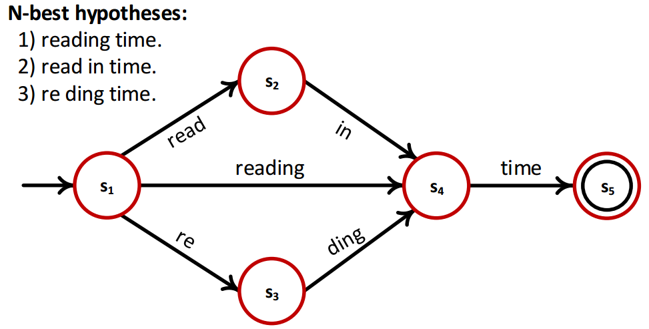
\includegraphics[clip=true, width=0.6\textwidth]{figure/lattice.png}
    \bicaption[fig:lattice]{}{N-Best候选序列和词图}{Fig}{N-Best Hypothesis and Lattices}
\end{figure}


由于N-Best候选序列中往往存在大量公共部分(比如图~\ref{fig:lattice}中的“time”这个词),因此将公共部分压缩在一起进行表示,也就是将多个候选序列转换成一张图来进行存储,将会更加高效。在语音识别中,这样一张图就称为词图。词图的生成所带来的额外操作与生成N-Best候选序列类似。具体来说,其往往要求在解码过程中做令牌合并时,保留多个历史记录。在记录完词图后,还需要词图剪枝步骤,其将冗余和无法连通边和结点删去,得到最终比较紧致的词图。

词图具有较多用途(一些例子如图~\ref{fig:lattice-usage}所示),因此相较于N-Best候选序列,词图的处理往往是语音识别系统中的一个标准模块。

\begin{figure}[!htp]
  \centering
    \captionstyle{\centering}
    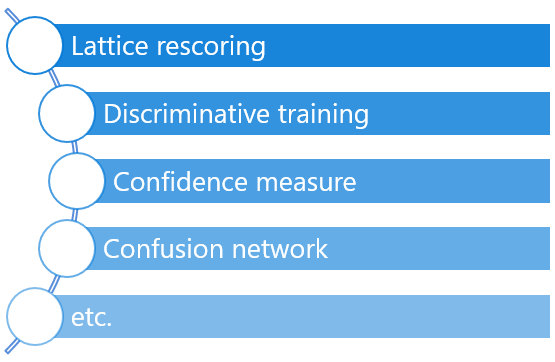
\includegraphics[clip=true, width=0.4\textwidth]{figure/lattice_usage.png}
    \bicaption[fig:lattice-usage]{}{词图用途举例}{Fig}{Applications of Lattices in ASR}
\end{figure}


\section{本章小结}
\label{chap:intro-sum}

在这章中我们简要介绍了语音识别的基本内容,首先讨论了特征提取,包括MFCC,PLP,FBANK等三种语音识别中常用特征;接着介绍了语音识别中最成功的声学模型——HMM以及利用最大似然估计和序列鉴别性准则来优化HMM模型;继而讨论了现实语音识别系统中的声学单元和参数绑定;最后讨论了N元语言模型和Viterbi解码等内容。

同时,本章回顾了语音识别推理阶段搜素解码部分基本内容和方法。
解码器对声学模型计算出的声学特征概率和语言模型计算出的语言概率进行组合来得到最大概率词序列。
%
在语音识别推理阶段,解码器是语音识别系统核心和灵魂,所有的信息都汇集于此。它将不同来源、 不同层次、 不同性质的知识和信息关联在一起,使它们互相之间取长补短, 从而得到正确语音识别结果。因此,如何将各种性质相异信息有机融合是解码网络和解码算法设计中必须认真研究和解决问题。
从解码器的作用来看,它既是语音识别研究中验证各种理论、模型、算法的
正确性的基本实验平台,也是构建实用系统的基础。因此,在解码器的设计中也
需要兼顾研究的方便与工程实际应用。

\chapter{语音识别中的解码搜索问题}
\label{chap:intro2}

本章中,我们首先介绍基本的维特比解码搜索算法,而后引入其在语音识别中的应用。我们对语音识别中的解码搜索问题及其当前解决方案进行了详细介绍。这些不同的技术流派包括同步和非同步之分,以及动态和静态之分。我们对近十年主流的加权有限状态机技术进行了重点介绍。基于上面的介绍,我们总结了当前解码器研究中的待解决问题,以及上一章中深度序列学习模型所带来的研究机遇。后续本论文的一系列工作将基于本章针对解码器的分析,讨论和总结。


\section{维特比解码搜索算法}
\label{chap:intro2-viterbi}

维特比算法是一种动态规划算法,用于寻找维特比路径,其对应于最有可能产生观测事件的序列,即隐含状态序列。这一算法最早由安德鲁·维特比(Andrew Viterbi)在1967年提出,用于在数字通信链路中解卷积以消除噪音。 此算法被广泛应用于GSM和CDMA数字蜂窝网络、拨号调制解调器、深空通信、卫星和802.11无线网络中的解卷积码。另一大类应用为计算语言学和生物信息学,以及语音识别和关键字检测。例如在语音识别中,声音信号作为观察到的事件序列,而文本字符串,被看作是隐含的产生声音信号的给定原因,因此可对声音信号应用维特比解码搜索算法寻找最有可能的文本字符串序列。

假设给定隐式马尔可夫模型(HMM)状态空间 S, 初始处于状态i 的概率 $\pi_{i}$ 以及转移概率 $a_{i,j}$,其对应于从状态i转移到状态j的概率。同时我们观测到输出序列 $y_{1},\dots ,y_{T}$。 其对应的产生该观察序列的相应隐状态 $x_{1},\dots ,x_{T}$ 可以由递推关系得到。

\begin{equation}
\begin{split}
V_{1,k}=\mathrm {P} {\big (}y_{1}\ |\ k{\big )}\cdot \pi _{k}
\end{split}
\end{equation}
\begin{equation}
\begin{split}
V_{t,k}=\max _{x\in S}\left(\mathrm {P} {\big (}y_{t}\ |\ k{\big )}\cdot a_{x,k}\cdot V_{t-1,x}\right)
\end{split}
\end{equation}

\begin{equation}
\begin{split}
V_{1,k}=\mathrm {P} {\big (}y_{1}\ |\ k{\big )}\cdot \pi _{k}
\end{split}
\end{equation}
\begin{equation}
\begin{split}
V_{t,k}=\max _{x\in S}\left(\mathrm {P} {\big (}y_{t}\ |\ k{\big )}\cdot a_{x,k}\cdot V_{t-1,x}\right)
\end{split}
\end{equation}

这里的$V_{t,k}$表示前 t 个最终状态为 k 的观测结果最有可能对应的状态序列的概率。通过保存向后指针记住在第二个等式中用到的状态 x 可以获得维特比路径。声明一个函数$\mathrm {Ptr} (x_{t},t)$ ,它返回若 $t>1$ 时计算 $V_{t,k}$ 用到的 x 值 或若 $t=1$ 时的 k,这样:


\begin{equation}
\begin{split}
x_{T}=\arg \max_{x\in S}(V_{T,x})
\end{split}
\end{equation}
\begin{equation}
\begin{split}
x_{t-1}=\mathrm {Ptr} (x_{t},t)
\end{split}
\end{equation}
\begin{equation}
\begin{split}
x_{T}=\arg \max _{x\in S}(V_{T,x})
\end{split}
\end{equation}
\begin{equation}
\begin{split}
x_{t-1}=\mathrm {Ptr} (x_{t},t)
\end{split}
\end{equation}

这里我们使用了arg max的标准定义,算法复杂度为 $O(T\times \left|{S}\right|^{2})$。一个更好的估计存在于迭代只针对那些可以连接到当前状态的下一个状态当中,那么算法复杂度为 $O(T\times (\left|{S}\right|+\left|{E}\right|))$,其中的E 表示图中所存在的边数。

\section{语音识别中的解码搜索问题}
\label{chap:intro-asr-dec}

语音信号的识别既是一个模式识别问题,也包含相应的推理搜索问题。前一个问题对各种语音信号的、语言现象进行数学表示和描述,在基于统计学习的模式识别框架下进行建模,这决定了语音信号的识别系统可达到识别准确度的上限。而后一个问题在给定模型情况底下,研究如何高效地将输入语音信号的和模型相匹配,推理搜索得到最优识别结果,这决定了识别速度和实际可达的识别准确度。
在语音信号的识别的推理搜索阶段,解码器功能是对声学模型计算出的声学特征概率和语言模型计算出的语言概率进行组合来得到最大概率的词序列。

在语音识别中,声音信号作为观察到的事件序列,而文本字符串,被看作是隐含的产生声音信号的给定原因,因此可对声音信号应用维特比解码搜索算法寻找最有可能的文本字符串序列,称为语音识别的推理搜索阶段。
%
在语音信号的识别推理搜索阶段,解码器是语音信号的识别系统的核心和灵魂,所有信息都汇集于此。它将不同来源、 不同层次、 不同性质的知识和信息关联在一起,使它们互相之间取长补短, 从而得到正确的语音信号的识别结果。因此,如何将各种性质不同的信息有机融合是解码网络和解码算法设计中必须认真研究和解决的重要问题之一。
从解码器的作用来看,它不仅是验证语音信号识别中各种理论,模型和算法正确性的基本实验平台,也是构建实际系统的基础。因此,在解码器设计中,还必须考虑到研究的便利性和工程的实际应用。

语音识别系统可以分为关键词检测,孤立词识别,语法网络识别,大词汇连续语音识别和基于神经网络语音模型的大词汇连续语音识别,下面我们将对它们中的解码搜索问题进行逐一介绍。

\subsection{关键词检测和孤立词识别}
\label{chap:intro-kws-dec}

%综述关键词检测
关键词检测(KWS)是语言识别最主要的应用之一,它的目标是得到一个高准确度和高效率的识别器,用于检测特定的一些关键词在语音中的出现。
KWS可以被用于声学数据挖掘~\cite{zhou2005data}, 低资源的音频检索~\cite{shen2009comparison}, 
语料库检索~\cite{garofolo2000trec} 和 唤醒词识别~\cite{chen2014small}。

KWS 技术可以被分为两大类:
i) 非监督的  {\em query-by-example} (QbyE) \cite{zhang2009unsupervised,barakat2012improved,chen2015query}, 它使用了关键词的声学样例来产生一系列模板,之后尝试将模板与测试音频样例进行匹配来决定是否被唤醒。
ii) 监督的基于文本的方法,这部分可以被进一步分类为  基于{\em 大词汇连续语音识别} (LVCSR)  方法 ~\cite{garofolo2000trec,ng2000subword} 和  {\em 声学 KWS} \cite{mandal2014recent}。
对于前者,在训练阶段需要构建一个词,半词或音素的语音识别系统。声学和语言模型在测试阶段一起对语音进行转录并得到词图。之后在词图上进行关键词搜索得到最终的结果。
声学 KWS 不需要语言模型,通过直接建模目标关键词,半词或音素,构建一个声学模型来进行关键词的判别。一些方法中也会考虑引入非关键词元素到建模当中~\cite{sukkar1996utterance}。
QbyE 主要用于低资源音频检索, 本文不针对这个方向。 
在 语料库检索中, 基于LVCSR方法通常能得到更好的性能,相比声学KWS。但是基于LVCSR方法也有如下一些缺点: 需要训练一个非常通用的大词汇连续语音识别系统,因此需要大量语料;同时在测试阶段也需要非常大的词表进行覆盖。这样的缺点限制了它在一些应用,比如唤醒词识别中的应用。除此之外,基于LVCSR的方法忽略了KWS任务本身的一些特性,该类方法的推理搜索阶段解码搜索算法主与大词汇连续语音识别中类似,详细讨论参加下一章节。

在声学关键词检测中,模型通常是进行逐帧分类的。解码方法用于解决模型所造成的误唤醒问题。解码的搜索空间通常包含两个部分:领域内搜索空间和领域外搜索空间。前者由关键词序列得到,而后者通常可以由特定模型进行建模(比如后文将提到的$filler$模型)领域外的搜索空间。另一方面如果KWS建模不是直接针对关键词,而是针对关键词的子序列,则搜索空间还需要建模子序列与目标关键词之间的映射关系(比如词典和发音序列)。

%综述孤立词识别
孤立词识别是指对用户单个词语孤立发音的语音识别。
在特定人孤立词语音识别中,最为简单有效的方法是采用动态时间规整(Dynamic Time Warping,DTW) 算法,该算法基于动态规划的思想,解决了语音长短不一的模板匹配方面的问题,是语音识别中出现最早且较为经典的一类算法。这类算法依然基于动态规划和维特比搜索解码。DTW通过把时间序列进行延伸和缩短,来计算两个时间序列性之间的相似性。其计算遵循一定的搜索规则,根据语音信号在时间上的连贯性,认为所有路径均是从第一帧出发,并在最后一帧和最后一个输出上结束。由于两序列之间不等长,所以需要在匹配过程中限定弯折率来实现。最优路径为在满足约束条件下,计算路径累计距离的最小值。



\subsection{语法网络识别和大词汇连续语音识别}
\label{chap:intro-lvcsr}

%语法网络
孤立词的语音并不是人类沟通的自然方式。为了建模人类的自然语言,一种方法是使用语法网络来进行语音识别。
语法网络可以规定词语按照什么规则来合成句子,即概率式句法结构。
在该网络中,每个句子由若干词条组成,每一个词条都选自词汇表。句子中一个要选择的词条以一定的概率出现,而选择第二个词条的概率与前一个词条出现的概率有关,以此类推,直到句子的结束。在此框架里,每一个词语由若干个音素串接而成。而后每一个音素用一个HMM模型以及一套参数来表示。每一个HMM模型中最基本的构成单位是状态与状态之间的转移弧以及每个状态的概率建模。这样,从HMM状态出发逐层扩大到音素、词语、句子。每一个句子是包含许多状态的复杂的状态图,该句子就是用所有状态形成的结构、状态之间的转移概率,以及每个转移弧产生某个特征输出的概率来描述。对于特定的词表和句法,所有可能出现的句子构成一个更大的状态图。在完成识别任务的时候,要根据一个输入语音特征矢量序列来确定一个最可能的句子。这就需要在这个大的状态图中搜索一条路径,该路径上产生上述特征矢量的概率最大,有路径可以进一步确定句子中的每一个词。这种路径搜索就是采用维特比搜索算法。

语音识别中更具有挑战性的研究课题则是大词汇量、非特定人的连续语音识别,称为大词汇连续语音识别。
大词连续语音识别中,语音信号先经过分析后形成特征矢量,并按隐马尔科夫模型,上下文音素,字典和词模型,语言模型结合而成的搜索空间进行识别,最后得到相应的句子。

与关键词检测和孤立词识别相比:传统语音识别模型要针对整个短语序列进行识别显然是不可能的,因为语言中短语的数量太多,所以必须把输入的语流切分为更小的组分来进行,相比较人类感知语音的过程也是类似的。由于连续语音中间没有间歇,所以在识别前必须先把各字拆分开,这就需要系统必须能够识别单词之间的边界关系。但这是非常困难的,因为确定单词间的边界位置还没有现成的方法来进行。尽管有时候可以采用能量最低点作为边界的判断准则,但是通常要根据发音信息加以辅助验证。另一方面,连续语音的发音比孤立词的发音跟随便,受协同发音的影响也就更为严重。除此之外,连续语音识别系统中的很多问题都与相应的语言学知识有关,特别是大词汇连续语音识别系统要更多地强调运用语言学知识来进行。

另一方面,大词汇连续语音识别的解码过程复杂度非常高。解码搜索的复杂度与上述由隐马尔科夫模型一直到语言模型的各个层面相关。下面我们将举例子进行说明。
%在语音识别里搜索意味什么,词级,语法级,语言模型,神经网络级(search基本形态); 为什么难,复杂度多高;
首先在有限状态语法网络网络以及 unigram和monophone情况下,其语法网络如图~\ref{fig:exp-ug}所示。
该语法网络在每帧上的近似的复杂度包括两部分:
\begin{enumerate}
\item 内部传递: $W_{\tt ug}\times P\times N$, 其中 $P$ 是每个词的平均音素数量, $N$ 是每个模型的状态个数
\item 外部传递: $W_{\tt ug}\times P + W_{\tt ug}$ 
\end{enumerate}
而扩展到unigram的情况,在每一个词的开始,将unigram的概率加到令牌的对数似然度上,使得语言模型的信息尽可能早地合并进来。

\begin{figure}[!htp]
  \centering
    \captionstyle{\centering}
    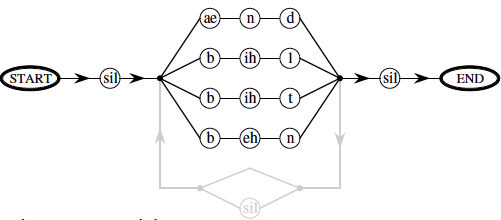
\includegraphics[clip=true, width=\textwidth]{figure/ug.png}
    \bicaption[fig:exp-ug]{}{有限状态语法网络网络以及 unigram和monophone}{Fig}{Finite State Grammar Newwork with unigram and monophone}
\end{figure}

而如果扩展到Bigram和monophone情况下,其语法网络如图~\ref{fig:exp-bg}所示。在每帧上的近似的复杂度则包括内部传递: $W_{\tt ug}\times (P+1)\times N$ 和 外部传递: $W_{\tt ug}\times P + W_{\tt ug}^2$。而如果使用回退back-off语言模型, 词传递大致是 $W_{\tt bg}+W_{\tt bo}\times W_{\tt ug}$。

\begin{figure}[!htp]
  \centering
    \captionstyle{\centering}
    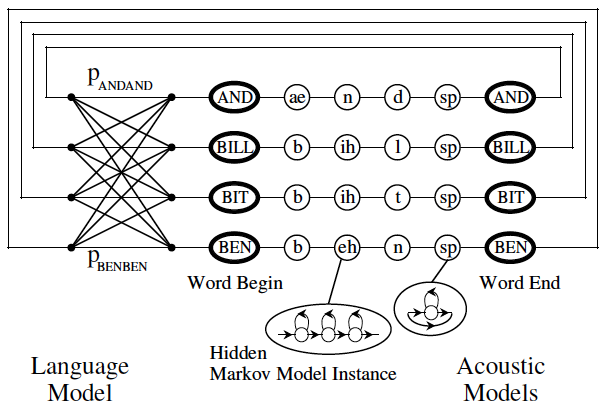
\includegraphics[clip=true, width=\textwidth]{figure/bg.png}
    \bicaption[fig:exp-bg]{}{Bigram和monophone的语法网络}{Fig}{Finite State Grammar Newwork with Bigram and monophone}
\end{figure}


再扩展到Bigram和cross-word triphone 情况下,其语法网络如图~\ref{fig:exp-xwrdbg}所示。在每帧上的近似的复杂度则包括内部传递: $W_{\tt ug}\times (P-2+ P_{\tt prefix}+ P_{\tt suffix})\times N$ 和 外部传递: $W_{\tt ug}^2 + W_{\tt ug}\times (P-2+ P_{\tt prefix}+ P_{\tt suffix})$。

\begin{figure}[!htp]
  \centering
    \captionstyle{\centering}
    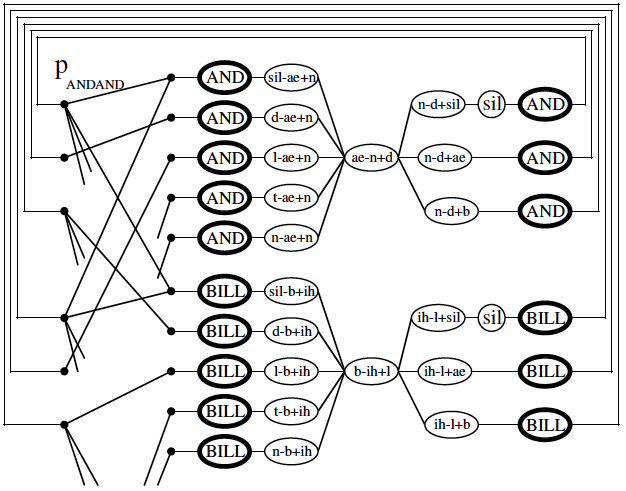
\includegraphics[clip=true, width=\textwidth]{figure/xwrdbg.png}
    \bicaption[fig:exp-xwrdbg]{}{Bigram和cross-word triphone的语法网络}{Fig}{Finite State Grammar Newwork with Bigram and cross-word triphone}
\end{figure}

如果使用Trigram和within-word triphone,其语法网络如图~\ref{fig:exp-tg}所示。在每帧上的近似的复杂度则包括内部传递: $W_{\tt ug}^2\times (P+1)\times N$ 和 外部传递: $W_{\tt ug}^3 + W_{\tt ug}^2\times (P+1)$。
如果是回退back-off LM, 词传递大致是$W_{\tt tg}+W_{\tt bo}^{\tt bg}(W_{\tt bg}+W_{\tt bo}W_{\tt ug}) $。

目前业界最主流的系统使用trigram语言模型和跨词三音子triphone声学模型,该情况下,解码复杂度会变得甚至更大。因此在下一章节中我们将介绍如何在复杂度如此之高的搜索网络上进行解码搜索。

\begin{figure}[!htp]
  \centering
    \captionstyle{\centering}
    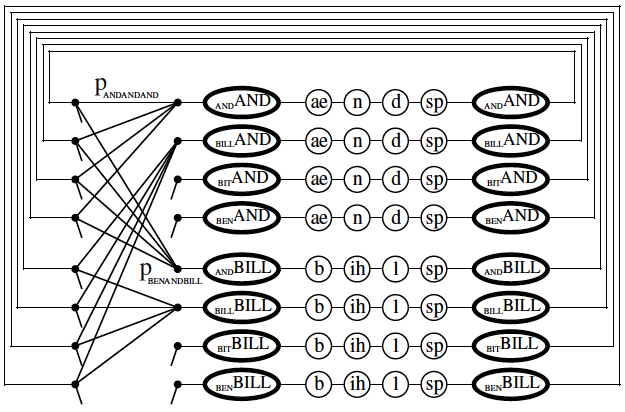
\includegraphics[clip=true, width=\textwidth]{figure/tg.png}
    \bicaption[fig:exp-tg]{}{Trigram和within-word triphone的语法网络}{Fig}{Finite State Grammar Newwork with Trigram and within-word triphone}
\end{figure}

\section{解码器技术综述}
\label{chap:intro2-dec-sum}

\subsection{解码器的技术流派}
\label{chap:intro-lvcsr-decmethod}

\subsubsection{静态和动态的搜索空间构建方法}
\label{chap:intro-lvcsr-decmethod-graph}

根据前面章节讨论,完整的语音信号识别系统由自下而上的五层映射关系组成:语音信号到HMM状态的观察,HMM状态到依赖于上下文的音素,依赖于上下文的音素到音素,音素到单词,单词到句子。
具体来说公式~\ref{eq:decode}可以进一步展开如下:
\begin{equation}
 \begin{split}
\mathbf{w}^* = \arg \max_{\mathbf{w} \in \mathcal{H}} \max_{\mathbf{s}} P(\mathbf{s}|\mathbf{w})p(\mathbf{O}|\mathbf{s})P(\mathbf{w}) \\
= \arg \max_{\mathbf{w}} \sum_{\mathbf{l}} \sum_{\mathbf{c}} \sum_{\mathbf{s}}
p(\mathbf{O}|\mathbf{s}) \cdot
P(\mathbf{s}|\mathbf{c})\cdot P(\mathbf{c}|\mathbf{l})\cdot P(\mathbf{l}|\mathbf{w}) \cdot 
P(\mathbf{w})
 \end{split}
\end{equation}
其中展开后式子每一项分别对应上述的五层映射关系。
在识别之前不能知道语音信号的观察,因此需要在解码过程中动态地建立观察到的语音信号的HMM状态的映射,并且还需要实时计算相应的声学分数。对于从HMM状态到依赖于上下文的音素,依赖于上下文的音素到音素,音素到单词的三级映射关系,一旦确定了发音字典和声学模型,它们就不会改变。为了追求解码效率,人们通常将它们静态编译成解码网络。对于没有任何约束的大词汇量连续语音信号的识别任务,可以以任何方式将单词组织成句子,因此原则上,单词 - 句子映射关系只能在解码过程中动态建立。然而,由于表征单词和单词之间的关联度(概率)的N-gram语法模型在解码之前已经存在并且是有限集,因此在实践中,语言模型得分计算可以以不同方式实现。在语音信号识别领域,根据解码器中语言模型的表示,语言模型状态获取和语言模型得分计算方法,解码器通常分为两大流派:
\begin{itemize}
\item 动态网络解码器: 在动态网络解码器中,解码网络仅包含发音字典和声学
模型,不会含有语言模型任何信息。 语言模型状态在解码过程中还要随着词与词相连
成句而动态地生成、语言模型分数通过去查表的方式动态地获取。这类解码器的典型
代表是基于发音前缀树(Pronunciation Prefix Tree, PPT)~\cite{woodland1994large}网络解码器。
\item 静态网络解码器: 在静态网络解码器中,解码网络不仅包含发音字典和声
学模型,也包含完整的语言模型分数。 语言模型状态以及状态转移以WFST的形
式合成到解码网络中去, 语言模型分数则作为状态转移概率存储于边上。解码时,
仅需逐边积累整条路径状态转移概率便可获得语言模型分数。这类解码器的典
型代表是基于加权有限状态转换器(WFST)~\cite{mohri2002weighted}的解码器。
\end{itemize}

作为一种时空变换策略,静态网络解码器通常可以通过仔细优化实现更快的识别速度,但缺点是显而易见的:构建的解码网络太大,特别是在高阶语言中。在模型和声学模型的情况下,由于存储器大小限制,将所有知识源编译到解码网络中通常是不可行的。因此,近年来,基于动态解码网络的传统解码信号的识别方法逐渐受到研究者的青睐~\cite{soltau2009dynamic,rybach2011comparative}, 能够几乎不受任何约束地利用更高阶语言模型和声学模型以便获得更优异的识别准确度, 应用面更广, 这是动态网络解码器最为吸引人的地方。然而动态网络解码器的设计和束搜索剪枝方法更加复杂,需要调整参数和阈值更多,挑战性更大。 

\subsubsection{同步和异步的搜索算法}
\label{chap:intro-lvcsr-decmethod-search}

除了根据解码网络的结构进行分类之外,还可以根据搜索最优路径的不同方式将解码器划分为时间异步搜索解码器和时间同步搜索解码器:

\begin{itemize}
\item 时间异步搜索解码器: 在较老的解码器,例如: IBM ViaVoice 中, 采用深度优先方式在解码网络中搜索最优词序列, 是一种时间异步搜索。由于这类解码
器在解码过程中需要用到一些后进先出的缓冲区(即:堆栈)来保存扩展得到词识别假设,所以也常常被称为堆栈解码器(Stack decoder)~\cite{paul1992efficient}。 
与时间同步搜索相比,优点在于通过选择适当的启发函数,搜索可以控制于最佳路径附近,并且提高了搜索效率。但这也造成了它的主要缺陷:1)启发函数综合声学和语言分数,有时需要“未来”路径信息,因此很难获得; 2)因为它是时间异步搜索,所以搜索过程产生的路径长度各不相同,使得修剪很难实现。因此,当前的堆栈解码很少用于直接解码语音信号的观察,而更多地用作用于从字图生成N-Best结果的后处理中。
\item 时间同步搜索解码器:时间同步搜索是目前解码器设计和实现的主流方法,也称为帧同步搜索。它使用广度优先方法找到与来自解码网络的输入特征序列最佳匹配的状态序列,以便获得相应的最佳音素序列和字序列。这种类型的解码器通常使用维特比算法或令牌传递算法~\cite{woodland1994large}实现。 
\end{itemize}

时间异步的搜索算法还包括多遍解码算法。多遍解码算法通常在每次解码过程中对之前的搜索空间进行剪枝,缩小空间大小,而后将压缩后的搜索空间交给下一次解码算法,进行进一步搜索,直到最终得到最佳结果。
为在搜索中利用各种各样的知识源,通常要进行多遍搜索,第一遍要使用代价较低的知识源,产生一个候选序列列表或词候选网格,在此基础上再进一步进行使用代价高的知识源的第二遍搜索来得到最佳路径。这里的知识源包括声学模型、语言模型和音标词典,这些可以用于第一遍搜索。为实现更准确的语音识别,往往要利用一些代价更高的知识源,如高阶的上下文相关的N-Gram语音模型、词间混淆相关模型、分段模型或语法分析算法,进行重新打分。目前主流的实时大词汇连续语音识别系统许多都使用这种多遍搜索策略。
与单遍搜索(1-pass)相比,多遍搜索具有优点和缺点,并且它也在实践中使用。多遍搜索的支持者认为:第一遍粗搜索可以大大减少解码空间,使得在后续解码过程中使用更精细的语言模型和声学模型成为可能,避免了单遍解码器中的时间和空间限制。 。单遍搜索的支持者认为在多遍解码中存在三个主要问题:1)由于第二遍解码必须等待第一遍解码,因此多遍搜索难以应用于实时解码。 2)每次通过解码引入了不可恢复的修剪误差,其不能被后续解码中使用的任何模型补偿。要解决这个问题,我们仍然需要努力研究单遍搜索算法。最好直接进行单遍解码器。 3)多次解码器的每次解码中使用的特征,声学模型,语言模型和搜索算法是不同的。

解码器不仅算法复杂,而且需要高工程能力和技能。在开发完成后,通常需要大量的人力和时间进行调整。因此,各种研究机构和商业公司都有自己的解码器实现细节。它就像它一样深。尽管如此,世界上仍有一些用于学术研究的开源解码器可以作为研究的基础。该表列出了比较知名的那些。这些解码器的网络结构和解码算法不同,但由于学术研究的目的,大多数速度优化都比较差。


\begin{table}[thbp!]
  \caption{\label{tab:perf-compare} {\it  知名开源解码器 } }
  \centerline{
    \begin{tabular}{c c  c c}
      \toprule
      解码器 &  研发机构 & 网络结构 & 搜索算法 \\
      \midrule
      HDecode & 英国剑桥大学 & 动态,发音前缀树 & 单遍, 令牌传递 \\
        Sphinx &美国卡内基梅隆大学 &动态,发音前缀树 &单遍, 令牌传递 \\
        RASR &德国亚琛工业大学& 动态, 发音前缀树 &单遍, Viterbi \\
        Juilus & 日本京都大学 & 动态, 发音前缀树 & 两遍, 前后向搜索。\\
        Juicer & 瑞士IDIAP & 静态, WFST & 单遍,令牌传递 \\
        Kaldi & 美国约翰霍普金斯大学 & 静态, WFST & 两遍,令牌传递     \\
\bottomrule
    \end{tabular}
  }
\end{table}


\subsection{主要模块和核心算法}
\label{chap:intro-lvcsr-decmodule}

\subsubsection{解码器框架}

图~\ref{fig:dec_arch}给出了典型解码器结构。不论是哪种类型解码器通常都包含网络生
成、分数计算、搜索、剪技与路径管理这五部分,它们的功能逐一介绍如下。

\begin{figure}[!htp]
  \centering
    \captionstyle{\centering}
    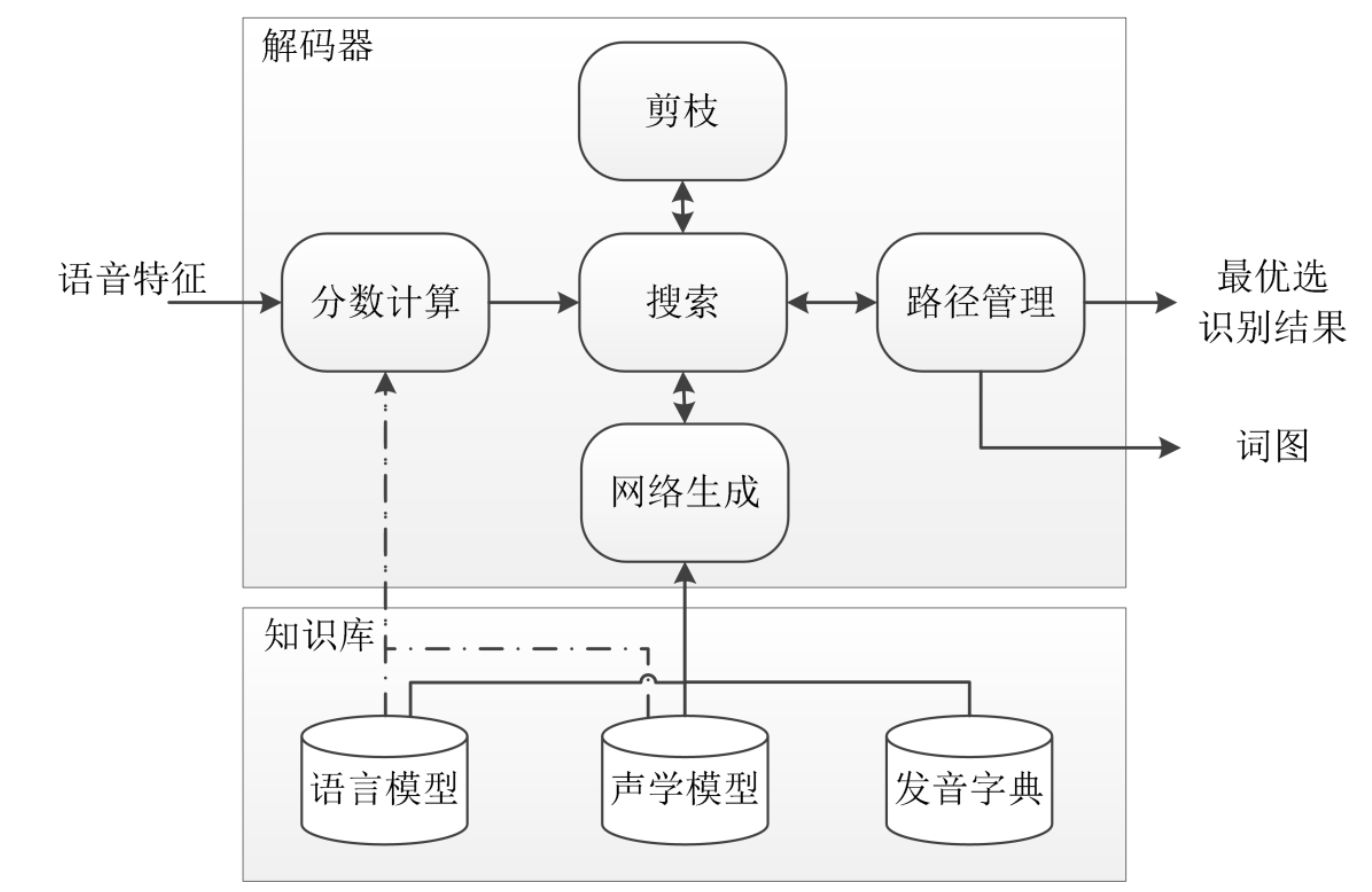
\includegraphics[clip=true, width=.9\textwidth]{figure/dec_arch.png}
    \bicaption[fig:dec_arch]{}{通用解码器架构}{Fig}{General Architecture of ASR Decoder}
\end{figure}


\subsubsection{基于加权有限状态机的网络生成算法}

网络生成模块主要负责构建解码搜索空间。搜索空间(也称为解码网络)通常与音素HMM或HMM状态连接,从语言模型,发音词典,声学模型和其他相关知识源编译。大词汇量连续语音信号解码网络的识别系统由各种知识源组成,形成搜索空间,一般可分为动态构造的解码网络和静态网络。基于动态网络解码器,前缀树发音字典用作搜索网络。语言模型通过动态查询将得分引入解码过程,然后通过重新输入字典树或字典树副本来搜索整个解码网络~\cite{young2002htk}。
动态网络解码器主要优势在于,由于字典和语言模型是分离,其占用内存极少,这个特点在以往移动网络技术和硬件技术不发达的时代,尤其是在嵌入式设备上内置解码器的时代,占有着绝对优势。但是动态网络的缺点是它解码速度较慢,时间复杂度较高,这也使其愈加难以满足当前海量语音信号的识别请求。
随着移动互联网和嵌入式设备的普及以及云技术的发展,语音信号的识别应用已发展为仅在嵌入式设备上保持简单的前端,而识别系统仍保留在服务器云中。此时,反映了基于WFST的静态网络解码器的快速优势。较短的识别时间允许服务器每单位时间接受更多的识别任务,因此静态编译的解码网络更适合于大量语音信号识别任务。

在LVCSR任务中,解码网络通常非常大。因此,网络结构需要采用各种手段来优化网络结构,并在不改变网络功能的情况下尽可能地减少网络中的节点和边数量。解码网络是解码器的基础,并确定在解码器的其他部分中应该使用哪种方法。在静态网络解码器中,解码网络不仅包含发音字典和声学模型,还包含完整的语言模型。语言模型状态和状态转换以有限状态机的形式合成到解码网络中,并且语言模型得分被存储为边上的状态转移概率。当解码时,仅通过累积整个路径状态转移概率可以获得语言模型得分。这类解码器的典型代表是基于加权有限状态转换器(WFST~\cite{mohri2002weighted}的解码器。

WFST最开始由AT\&T实验室Mohri和Riley等人在1997年引
入语音信号的识别领域。并且在理论上发展了确定化、最小化等一系列网络优化算法,为语音信号的识别的应用打好了理论基础。语音信号的识别各模型组件分别用如下方式进行WFST构建:

\begin{itemize}
\item N-gram语言模型在WFST中表示为G.根据N-gram语言模型的含义,它提供了单词历史的当前单词概率。语言模型需要具有记录最多N个单词的历史的信息。但是,当识别语音信号时(即,输入和输出是其符号集的单个元素),WFST应用程序不允许使用字符串输入和输出。因此,不可能在G构造过程的输入和输出上表达其历史,而是记录该状态的历史。另一个问题是N-gram模型的回退(Back-off),当语言模型训练语料未出现某一个N元词组的时候,就会以一个回退的(N-1)元模型概率乘以一个系数来替换。这部分表示为一个带有着权重但是输入为空的状态跳转边。

\item 字典在WFST中被表示为L。
字典实际上是发音规则的表示。最简单的方法是列出开始状态和结束状态之间每个单词的发音。同时,由于在与语言模型合成时连接了单词和单词,因此无法达到终止状态,并且需要将闭合边从终止状态连接到开始状态以形成闭环。针对字典的同发音问题,Mohri在文献~\cite{mohri2002weighted}中提出对于不同词的同发音发音
序列加入一组辅助符号,这样对于同发词语,其环路的输入符号序列就不再相同,可以确保字典的可确定化。

\item 上下文相关声学模在WFST中被表示为C。
一个上下文相关triphone模型一般表示为a-b+c,其中b是中心音素,
a和c为其前后上下文音素~\cite{seide2011conversational}。用WFST表示triphone模型实际上是在把三音素和单个音素之间进行对应,其输出就和发音字典的输入做相互对应,由此可以进行进一步合成。

\item 隐马尔可夫模型在WFST中被表示为H。
HMM模型天然具有多个的状态跳转特性,所以可以直接将其构建为多个WFST状态。隐马尔科夫模型的转移概率于是被转化为WFST的权重。而WFST输入是隐马尔科夫模型的状态索引,输出是该隐马尔科夫模型所表示的triphone建模单元。
\end{itemize}

当各个知识源WFST组件被构建完毕以后,可以利用WFST合成算法和优化算法将各组件最后进行合并和最终优化。如下:
\begin{equation}
HCLG = min(det(H \circ min(det(C \circ min(det(L \circ G))))))
\end{equation}

最终生成的WFST包含了所有的知识源,后文所讨论维特比搜索就在它上面进行。

\subsubsection{分数计算}

分数计算模块计算输入特征序列声学和语言分数,并将它们提供给搜索模块以供使用。应该计算哪个分数与解码网络结构和搜索算法有关。例如,在静态网络解码器中,语言模型得分已经被编译到解码网络中,因此只需要计算声学得分;对于动态网络解码器,除声学分数外,还需要计算语言模型分数。分数计算的研究主要集中在如何实现分数的快速计算。对于声学分数,通常执行以下三个方面:

\begin{itemize}
\item 硬件加速。利用 CPU 矢量计算器~\cite{kanthak2000using}
或者通用图形处理器(Graphics Processing Unit, GPU)~\cite{chong2009fully}
加速分数计算。这类方法通常来说不会带来计算误差(与硬件实现相关),所以对识别准确度没有影响。
\item 模型简化。采用复杂度更小、参数更少的分类器模型,或通过聚类和参数共享减
小模型复杂度。例如采用半连续 HMM~\cite{huang1990semi} 替代连续 HMM,以及传统的参数共享方式~\cite{young2002htk}亦属此类。这类算法一般都会带来识别准确度上面的损失,所以需要在
识别准确度、模型复杂度和计算速度之间做好一定的权衡。
\item 算法优化。 对声学分数的计算过程进行简化。这类方法一般是对声学分数进行近似计算,所以必然会带来一定识别准确度损失。一般而言, 衡量一个近似算法是否可用的标准是看其带来相对识别准确度损失是否可控制在5\%以内~\cite{cai2009efficient}。
\end{itemize}

对于语言分数计算,当采用 N 元文法模型时,通常从两个方面进行加速: 1)
减小每次查表操作上面的耗时,典型方法是采用最小完美哈希(Minimal Perfect Hash,
MPH)表实现语言模型的存储与查取~\cite{li2007fast,cardenal2002fast}; 2) 引入分数缓存~\cite{huijbregts2008fast}减少查表熵的次数。

\subsubsection{维特比搜索}

搜索模块负责在解码网络上搜索得到最优路径。不论是静态网络解码器还是动态网络解码器,目前都以令牌传递算法~\cite{young1989token}为主流的搜索算法。

令牌传递是维特比算法的另一个更通用和简单的实现。在算法中,每个HMM状态可以与令牌(Token)相关联,令牌存储令牌所经历的历史路径和路径得分直到当前帧。解码是根据状态转换(即,沿着解码网络的边)将令牌从解码网络的初始状态传递到终止状态的过程。每个帧令牌向前传递一次,同时传递令牌得分和路径信息,并在多个令牌同时传递到状态时进行令牌合并,仅保留具有最高得分的令牌。在处理完所有帧之后,获得最佳路径和最佳路径得分。

令牌传递算法的优点是可以方便地在令牌上保存其他信息以便在状态节点之间进行传递,从而实现更复杂解码过程,例如: 为了生成词图,在令牌合并后, 不是将次优令牌直接丢弃,而是作为其他候选路径保存于合并后的令牌之上。

\subsubsection{剪枝}

在LVCSR中,搜索空间太大而无法对整个解码网络执行完全搜索。剪枝用于消除解码过程中的低分数路径,从而减少计算量并确保不降低识别性能。根据解码器设计,剪枝可以应用于搜索的各个阶段(例如,开始或结束),或者可以应用于各种级别(例如,单词级别,音素级别,状态级别,令牌级别),但是可以归纳为两个基本类别:

\begin{itemize}
\item 束剪枝(Beam pruning) :束剪枝保留与最优路径分数较近的次优路径。
令 $v(t,j)$ 表示第 t 帧位于状态 j 最优路径分数,则第t 帧的最优路径分数为:
\begin{equation}
v_{max}(t)=max_s v(t,s)
\end{equation}

令 $f$ 为剪枝阈值(又称为束宽),则束剪枝只保留所有满足下式的路径:
$v(t,j)>v_{max}(t)\cdot f$
\item 直方图剪枝(Histogram pruning) :与束剪枝不同,直方图剪枝仅保留分
数最高 N 条路径, N 为设定剪枝阈值。之所以称为直方图剪枝是因为该方法
可以采用直方图统计高效地实现~\cite{pylkkonen2005new}。
\end{itemize}

\subsubsection{路径管理和词图}

路径管理模型主要作用是用于对搜索过程中得到的路径链表进行回溯,获取最优路径、
N-Best 结果和词图。同时,它也负责对剪枝过程中所剪掉的较差路径进行内存回收等操作。

\begin{figure}[!htp]
  \centering
    \captionstyle{\centering}
    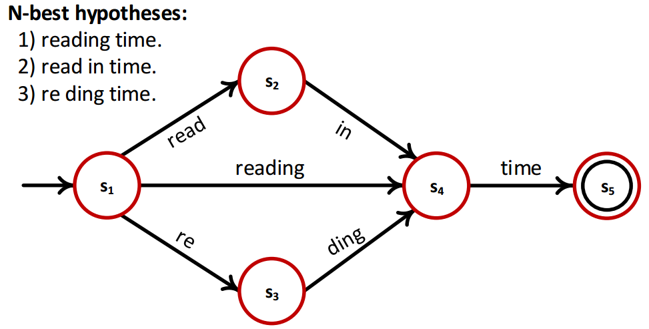
\includegraphics[clip=true, width=0.6\textwidth]{figure/lattice.png}
    \bicaption[fig:lattice]{}{N-Best候选序列和词图}{Fig}{N-Best Hypothesis and Lattices}
\end{figure}


由于N-Best候选序列中往往存在大量的公共部分(比如图~\ref{fig:lattice}中的“time”这个词),因此将公共部分优化在一起进行表示,也就是将多个候选序列转变成一张图来进行存储,将会更加紧致。在语音信号的识别中,这样一张图就称为词图。词图的生成所带来的额外消耗与生成N-Best候选序列类似。具体来说,其往往要求在解码过程中做令牌合并时,保留多个历史令牌记录。在记录完词图后,还需要词图剪枝步骤,其将冗余和无法连通边及其相应结点删去,得到最终比较紧致的词图。

词图具有较多用途(一些例子如图~\ref{fig:lattice-usage}所示),因此相较于N-Best候选序列,词图的处理往往是语音信号的识别系统中的一个标准模块。

\begin{figure}[!htp]
  \centering
    \captionstyle{\centering}
    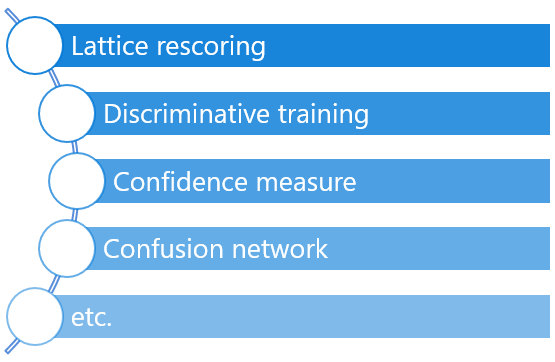
\includegraphics[clip=true, width=0.4\textwidth]{figure/lattice_usage.png}
    \bicaption[fig:lattice-usage]{}{词图用途举例}{Fig}{Applications of Lattices in ASR}
\end{figure}



\section{解码器研究中的待解决问题}
\label{chap:intro2-dec-future}
\subsection{研究现状总结}
\label{chap:intro2-dec-sumcur}

语音识别技术虽然相比多年以前已经有了长足的进步,但是在实际应用中还有很多困难需要处理。其中一个最主要难题就是语音识别推理搜索问题。
%
% 做什么事情
语音识别既是模式识别问题又是相应的推理搜索问题。前一个问题在数学上表示和描述了各种语音和语言现象,并且基于统计学习模式识别框架执行建模,该框架确定了语音识别系统可以实现的识别准确度的上限。在给定模型的情况下,后一问题研究如何使输入语音与模型匹配并推断最佳识别结果,其确定识别速度和实际可达到的识别准确度。在语音识别的推理搜索阶段,解码器功能组合声学模型以计算声学特征概率和语言模型计算的语言概率以获得最大概率词序列。
在语音识别推理搜索阶段,解码器是语音识别系统的核心和灵魂,所有信息都收集在这里。它将来自不同来源,不同层次和不同性质的知识和信息联系起来,以便它们相互补充并获得正确的语音识别结果。因此,如何有机地整合各种不同的信息是解码网络和解码算法设计中必须仔细研究和解决的问题。
从解码器功能的角度来说,它不仅是语音识别研究中各种理论,模型和算法的验证。
正确性和准确性的基本实验平台也是构建实际系统的基础所在。因此,在解码器的设计中必须平衡研究的便利性和工程的实际应用。


% 近来深度学习下发展现状和缺陷
近年来,深度学习模型被引入到语音识别声学和语言建模中以取代传统的分类器,显着提高了模式识别问题的准确性。在基于深度学习语音识别中,语音识别的推理搜索问题并没有得到根本改变。因为在该框架中,只有分类器得到了改进。
基于加权有限状态机(WFST)的推理搜索问题静态搜索空间构造技术~\cite{mohri2002weighted}和帧同步维特比(Viterbi)网络搜索算法~\cite{forney1973viterbi}仍是目前性能最好解决方案。该类系统存在的一系列显著缺陷包括:
\begin{enumerate}
\item 目前,语音识别系统基于多知识源建模结果,并对输入音频进行推理搜索。建模和推理搜索过程非常复杂,知识来源的划分依赖于强大的先验知识。大规模或非标记语音数据收集以及基于并行的深度学习技术使得构建直接模拟语音数据和文本序列的端到端模型及其相应的识别和推理搜索算法成为可能。当前的解码框架没有这种设计。
\item 
该种方案基于传统的混合高斯-隐马尔科夫模型(GMM-HMM)的声学模型和N元文法(N-gram)的语言模型而提出,针对目前性能最好的基于深度学习的声学模型和语言模型的研究并不充足,如何将新型的声学和语言模型引入该框架;如何充分发挥模型性能的同时改善推理速度;如何基于多知识源给出可靠的推理置信度算法,都是有待解决的问题。
\item 
该种方案基于对语音识别中各知识源(声学、语言、语义等)进行搜索空间的预先构建及整体优化,导致最终得到的搜索空间巨大,包括离线构建、在线使用、动态修改等各环节算法的计算量和内存消耗都非常大,是阻碍语音识别应用场景扩展的一个重要原因。旨在解决该问题,针对新型声学和语音模型的搜索空间整体优化研究尚不充分,而基于推理中间状态对搜索空间进行动态优化的研究几乎处于空白。
\end{enumerate}
因此,尽管基于深度学习模型,加权有限状态机和基于帧的维特比网络搜索算法的深度学习已经发展到基本可用水平,但是精度仍然不能满足人类之间的正常交流要求。速度限制也使得无法在低成本和低功耗的解决方案上工作,这些解决方案一起阻碍了语音识别技术的大规模商业应用。

\subsection{发展机遇和亟待解决问题}
\label{chap:intro2-dec-todo}
\begin{enumerate}
\item 基于并行计算提高解码搜索速度。

随着深度学习的发展和计算设备的个性,基于GPU的并行计算是一种潜在的针对语音识别计算的加速方式。针对声学模型推理,由于大部分计算量集中在矩阵形式的运算,因此它易于通过将类似于训练过程中\cite{vesely2010parallel}的序列批处理~\cite{dixon2009harnessing} 引入模型推理阶段,以加速运算速度。
但是,基于GPU并行计算的解码搜索并不容易实现。本质上它不再是一个易于并行的矩阵运算问题,而是一个图上最优路径的搜索问题。尽管一些研究在小型语言模型上取得了一定成功~\cite{you2009parallel},但这些系统仍然受制于两部分缺陷:i) 由于GPU显存有限,这些方法并不能有效利用较大的商用语言模型。
ii) 这些方法并不通用,常常受制于特定的声学或语言模型,并且没有词图生成功能。我们将在第~\ref{chap:gpu}章节对该方向进行研究。

\item 基于端到端建模降低解码搜索复杂度。

近来神经网络的发展使得更强的上下文和历史建模效果成为可能\cite{sak2014long,qian2016very}。同时,更多的标注数据也进一步缓解了模型的稀疏性和泛化问题。这些进展使得研究人员们有可能在更大的模型粒度上-从帧到整个序列层面~\cite{amodei2015deep,soltau2016neural,collobert2016wav2letter,sak2015fast,chan2016end}进行序列分解。在这些研究中,标签速率小于特征速率,但解码速率仍然等于特征速率。针对端到端模型的特性,特征层面的搜索过程可以考虑被修改为标签层面,即搜索空间是由不同历史的标签组成的,使得解码速率等于标注速率,从而小于特征速率。由于标签速率显著小于特征速率,这样做的好处是将带来搜索复杂度的大幅下降,从而得到搜索速度的大幅提升。我们将在第~\ref{chap:lsd}章节对该方向进行研究。

\item 基于端到端建模简化和统一解码推理框架。

由于不同ASR应用之间不同的搜索空间大小和效率要求,当前业界最优的置信度及其相应的解码算法在不同应用上具有不同架构,这些不同应用包括:关键词检测,基于上下文的语音识别和大词汇连续语音识别。要为所有的ASR应用设计一套统一的推理搜索框架,并取得最好的性能和速度,是一项非常有挑战的研究。这里面的关键点在于: i) 如何对最佳识别结果进行规范化,以得到对该最佳结果的置信度估计,也就是置信度中的归一化项的建模   ii) 如何保证在低功耗设备中的计算量控制在一个较小范围内,这对于置信度中的归一化项建模尤其具有挑战。借助上面提到的端到端建模,一方面可以对建模中的归一化项进行统一的较复杂的计算,另一方面可以有效降低上述计算中的复杂度。我们将在第~\ref{chap:unify}章节对该方向进行研究。


\item 基于端到端和序列建模提升解码搜索准确度。

语音识别是一种序列预测问题。除了需要研究如何将各种基于深度学习的模型方法应用到逐帧分类当中,使用序列级的鉴别性训练准则来强化模型的序列分类能力,也被证明是取得业界最好的大词汇连续语音识别系统的关键。但是关键词检测(KWS), 作为语言识别最主要的应用之一,几乎只受到了逐帧训练的深度学习的改善,却少有研究解决其鉴别性训练问题。
在上述的鉴别性训练中,对识别可能性的建模,即完整的搜索空间的建模是成功的关键。但是,在 KWS中,由关键词所定义的领域内搜索空间要显著小于领域外的搜索空间。因此领域外的搜索空间通常还需要特定的建模单元进行建模。
对领域外的搜素空间建模并不容易直接得到的问题,限制了序列鉴别性训练在关键词检测中的广泛应用。在第~\ref{chap:kws}章节中,我们在端到端建模和深度学习的框架下重新研究这一问题,以最终提升关键词检测系统的准确度。

\end{enumerate}
\section{本章小结}
\label{chap:intro2-sum}


本章回顾了语音信号识别和推理搜索阶段的搜索和解码部分的基本内容和方法。解码器将由声学模型计算的声学特征概率与由语言模型计算的语言概率组合,以获得最大概率词序列。在语音信号的识别和推理搜索阶段,解码器是语音信号识别系统的核心和灵魂,并且在此收集所有信息。它将来自不同来源,不同层次和不同性质的知识和信息联系起来,使它们相互补充,得到正确语音信号的识别结果。因此,如何有机地整合各种不同的信息是在解码网络和解码算法的设计中必须仔细研究和解决的问题。
从解码器的作用来看,它不仅是验证语音信号识别中各种理论,模型和算法正确性的基本实验平台,也是构建实际系统的基础。因此,在解码器的设计中,还需要考虑研究的便利性和工程的实际应用。

本章中重点总结了目前解码器的研究现状及存在的缺点和实现难点。后续几章我们的改进工作将具体针对所有这些目前存在的问题进行展开。



\chapter{关键词检测的序列建模和标签同步解码}
\label{chap:kws}

语音识别是一种序列预测问题。除了需要研究如何将各种基于深度学习的模型方法应用到逐帧分类当中,使用序列级的鉴别性训练准则来强化模型的序列分类能力,也被证明是取得业界最好的大词汇连续语音识别系统的关键。但是关键词检测(KWS), 作为语言识别最主要的应用之一,几乎只受到了逐帧训练的深度学习的改善,却少有研究解决其鉴别性训练问题。这里的主要原因来自鉴别性训练中的归一化项在KWS任务中不容易建模。
有少数研究尝试这一方向,但集中在固定关键词表的关键词检测或者基于LVCSR的关键词检测,并且它们也没有与当前主流的深度学习方法相结合。
在本章中,我们提出了针对固定或者非固定关键词的关键词检测系统的序列鉴别性训练框架。我们系统地研究了序列生成模型和序列鉴别模型情况下的序列鉴别性训练
通过引入词语无关的音素词图或非关键词的 {\em blank} 单元来构建竞争性搜索空间,我们在声学KWS系统上提出了一系列有效并且高效的序列鉴别性训练方法。实验表明我们提出的方法取得了一致并且显著的改善。这些测试包括固定关键词或非固定关键词的关键词检测任务,比较的基线是逐帧的深度学习声学KWS模型方法。

\section{引言}\label{Sec:kws-intro}

%KWS
%method categorized, what we discuss

关键词检测(KWS)是语言识别最主要的应用之一,它的目标是得到一个高准确度和高效率的识别器,用于检测特定的一些关键词在语音中的出现。
KWS可以被用于声学数据挖掘~\cite{zhou2005data}, 低资源的音频检索~\cite{shen2009comparison}, 
语料库检索~\cite{garofolo2000trec} 和 唤醒词识别~\cite{chen2014small}. 本文主要考虑后两种应用。


KWS 技术可以被分为两大类:
i) 非监督的  {\em query-by-example} (QbyE) \cite{zhang2009unsupervised,barakat2012improved,chen2015query}, 它使用了关键词的声学样例来产生一系列模板,之后尝试将模板与测试音频样例进行匹配来决定是否被唤醒。
ii) 监督的基于文本的方法,这部分可以被进一步分类为  基于{\em 大词汇连续语音识别} (LVCSR)  方法 ~\cite{garofolo2000trec,ng2000subword} 和  {\em 声学 KWS} \cite{mandal2014recent}。
对于前者,在训练阶段需要构建一个词,半词或音素的语音识别系统。声学和语言模型在测试阶段一起对语音进行转录并得到词图。之后在词图上进行关键词搜索得到最终的结果。
声学 KWS 不需要语言模型,通过直接建模目标关键词,半词或音素,构建一个声学模型来进行关键词的判别。一些方法中也会考虑引入非关键词元素到建模当中~\cite{sukkar1996utterance}。
QbyE 主要用于低资源音频检索, 本文不针对这个方向。 
在 语料库检索中, 基于LVCSR方法通常能得到更好的性能,相比声学KWS。但是基于LVCSR方法也有如下一些缺点: 需要训练一个非常通用的大词汇连续语音识别系统,因此需要大量语料;同时在测试阶段也需要非常大的词表进行覆盖。这样的缺点限制了它在一些应用,比如唤醒词识别,中的应用。除此之外,基于LVCSR的方法忽略了KWS任务本身的一些特性,改进这类方法主要跟改进大词汇连续语音识别声学建模相关。所以本章节主要研究声学KWS。

在声学关键词检测中,模型通常是进行逐帧分类的。目前研究趋势包括两方面:应用一个较强的逐帧分类器,比如深度学习模型,使最终系统带来性能提升~\cite{chen2014small,sainath2015convolutional}。 其次,语音识别本身是一个序列分类问题,传统的GMM-HMM系统在使用序列级准则,序列鉴别性训练时,往往能带来显著性能提升,比如discriminatively trained sub-word verification function~\cite{sukkar1996vocabulary}, minimum classification error (MCE)~\cite{sandness2000keyword} 和 performance-related discriminative training~\cite{keshet2009discriminative}。
在上述的鉴别性训练中,对对识别可能性的建模,即完整的搜索空间的建模是成功的关键。但是,在 KWS中,由关键词所定义的领域内搜索空间要显著小于领域外的搜索空间。因此领域外的搜索空间通常还需要特定的建模单元进行建模。
对领域外的搜素空间建模并不容易直接得到的问题限制了序列鉴别性训练在关键词检测中的广泛应用。
特别是在非固定关键词的关键词检测, 所以可能的竞争可能性通常无法被穷举,同时这种可能性的产生过程在使用LVCSR框架进行的时候~\cite{povey2005discriminative}非常耗时。 
%combination of both hasn't been carefully 

%Neural networks (NNs) for speech recognition are typically trained to classify individual frames based on a cross-entropy criterion (section 2.1).
在这篇文章中,我们为深度学习的 声学非固定关键词的关键词检测设计了相应的序列鉴别性训练方法。关于如何对序列概率进行定义,可分为序列条件似然度和序列后验概率,这包括两种序列模型: {\em 生成式序列模型} (GSM),比如HMM, 和 {\em 鉴别式序列模型} (DSM),比如 CTC。
对于GSM,序列鉴别性训练需要在序列上使用贝叶斯公式来通过序列条件似然度得到后验概率;而DSM则可以直接使用序列后验概率。

对这两种框架,竞争可能性的建模都是核心难题。
本章节提出两种方法来解决这一问题:隐性使用音素或半词单元的语言模型来建模,或者显性加入非关键词的标签。
%proposed KWS 
%Both frameworks are improved in the paper. 
在HMM中,受到近期一些研究中使用特点音素语言模型来对LVCSR的搜索空间进行建模的启发~\cite{povey2016purely,chen2006advances},  我们提出使用这种音素语言模型来对关键词的完整搜索空间进行建模。
为了加强关键词的鉴别能力,在关键词出现时候它们的梯度可以被增强。除此之外,许多神经网络结构和鉴别性训练准则也进行了详细比较。
在CTC中,非关键词建模单元被直接引入到建模当中。具体来说,加入之后的CTC模型搜索空间包括了关键词,音素边界 ($\tt blank$) 和词边界 ($\tt wb$)。 
最后我们基于前面章节介绍的LSD算法提出了一种高效的后处理算法,以解决音素混淆建模的问题。

本章节的主要贡献包括:
i) 针对生成式序列模型和鉴别式序列模型的序列鉴别性训练的第一个系统研究工作
ii) 提出了一些新颖的办法来构建声学KWS的竞争可能性,以用于鉴别性训练。这些方法显著提升了关键词检测系统的性能。
iii) 基于 LSD框架提出了高效的后处理方法,以便对音素混淆性进行建模。

\section{关键词检测的声学建模}
\label{Sec:kws-and-disc}

基于声学的关键词检测模型通常是要最小化每一帧的分类错误。在深度学习的HMM混合系统 (NN-HMM) 中,使用的是 tri-phone state作为建模单元,而深度学习模型则用来对每个HMM状态的后验概率进行建模。
特别是,对特征输入 ${\bf o}_{ut}$ 关于时间 $t$ 在句子 $u$中, 定义 $y_{ut}(s)=P(s|{\bf o}_{ut})$ ,表示神经网络在HMM 状态 $s$上的相应输出。这里的公式类似于GMM-HMM 系统~\cite{young1994state}, 除了需要使用伪对数似然度 $\log p({\bf o}_{ut}|s)$ 来针对HMM状态 $s$。
\begin{equation}
\label{equ:dnn-hmm-define}
\begin{split}
 p({\bf o}_{ut}|s) \propto \frac{ y_{ut}(s)}{ P(s)}
\end{split}
\end{equation}
公式中 $P(s)$ 是状态 $s$的先验概率。 
在深度学习系统中,如果建模单元是关键词,那么关键词 $w$ 的后验概率是要被直接训练得到的:
\begin{equation}
\label{equ:dnn-kw-define}
\begin{split}
P(w|{\bf o}_{ut})= y_{ut}(w)
\end{split}
\end{equation}
而前面讨论的后处理方法要被应用于逐帧的后验概率$y_{ut}(w)$上面。

%CE formula
这里通常可以使用负对数后验概率来作为交叉熵的目标函数。
\begin{equation}
\label{equ:dnn-hmm-ce}
\begin{split}
\mathcal{F}_{\tt{CE}}=- \sum_{u} \sum_{t} \log y_{ut}(s^{(r)}_{ut})
\end{split}
\end{equation}
公式中 $s^{(r)}_{ut}$ 是在时间 $t$ 句子 $u$ 上的标注,通过状态级强制对齐算法来得到~\cite{woodland1994large}。


\section{序列鉴别性训练}
\label{Sec:sdt-review}
由于语音识别本身是一个序列预测问题,所以序列级的准则往往能够带来性能的提升。依据序列的不同定义方式,目前有两种不同的序列鉴别性训练方法,一种针对  生成式序列模型 (GSM) 比如HMM,另一种针对 鉴别式序列模型 (DSM) ,比如 CTC 或者 encoder-decoder 模型。 
%序列鉴别性训练 for GSM is discussed in Section~\ref{Sec:sgm-sdt-intro} and DSM based 序列鉴别性训练 is discussed in Section~\ref{Sec:sdm-sdt-intro}.
 %while 序列鉴别性训练 in  CTC framework is considered in Section~\ref{Sec:kws-ctc}.

%table to show 
%       frame seq
%gen
%disc


\subsection{生成式序列模型 和 鉴别式序列模型 在ASR中的应用}
\label{Sec:sgm-and-sdm}
在语音识别中一个独有并且有趣的自然现象是声学序列和语言学序列的长度可变性。
序列模型正是被提出用来解决两个序列之间的关联性。大部分序列模型都包含一个用来对时序特性建模的部分, 比如GMM~\cite{woodland1994large} 和深度学习模型~\cite{hinton2012deep}用来对局部的声学特征进行建模,再加上一个对序列长度和转移进行建模的部分,比如HMM。近期提出的鉴别式序列模型, encoder-decoder~\cite{chan2016end}则尝试直接对序列建模而不是进行序列到逐帧的拆分。但在KWS中,性能和延迟在上述模型中都有一定限制。因此不参与本章节讨论。
本章节所有的序列鉴别性训练方法均基于逐帧的分解方式。基于模型是对条件似然度或者后验概率进行建模,概率模型通常可以分为生成式和鉴别式两种类型。值得注意的是在序列上或者在帧上,都可以使用生成式或者鉴别式进行分别建模,二者工作在不同层面上。
比如目前通常使用的混合 NN-HMM 模型就是采用生成式序列模型和鉴别式帧分类器。
在本章节中,我们主要关注序列模型。下文我们将比较模型结构和优化准则,在生成式和鉴别式序列模型中的异同。

 %There are two branches of sequence models. 生成式序列模型 is to model $P(\mathbf{O}|\mathbf{L})$ and 鉴别式序列模型 is to model $P(\mathbf{L}|\mathbf{O})$.

{\em 生成式序列模型}通常被定义为条件似然度$p(\mathbf{O}|\mathbf{L})$, 公式中 ${\mathbf O}$ 表示特征输入序列, $\mathbf L$ 表示标签输出序列。隐马尔可夫模型 (HMM) 是这类生成式序列模型的一个经典例子~\footnote{另一类 GSM 例子是Kalman 滤波器~\cite{digalakis1991dynamical,abbeel2005discriminative}.}. 
在NN-HMM 混合系统中, 语音信号的动态性使用HMMs 和来自深度学习模型的后验概率进行建模。
\begin{eqnarray}
\label{equ:hmm-model_2}
%\begin{split}
p(\mathbf{O}|\mathbf{L})&=&\!\!\!\!\!\!\sum_{\mathbf{q}\in\mathcal{A}(\mathbf{L})}\!\!\!p(\mathbf{O},\mathbf{q}|{\mathbf L}) =\sum_{\mathbf{q}}\prod_{t=1}^{T} p({\bf o}_{t}|q_t) P(q_t|q_{t-1})\nonumber\\
%y_{ut}(s^{(r)}_{ut})
&\propto&\sum_{\mathbf{q}}\prod_{t=1}^{T} \frac{P(q_t|{\bf o}_{t})}{P(q_t)}P(q_t|q_{t-1})
%\end{split}
\end{eqnarray}
公式中 $\mathbf{L}$ 表示标签序列,比如LVCSR中的词序列。
$\mathbf{q}$ 表示HMM状态序列,  $q_t$ 表示在帧 $t$上的HMM状态序列。 $P(q_t|q_{t-1})$ 表示 HMM 状态转移概率, $P(q_t)$表示状态的先验概率。
$\mathcal{A}$表示由标签序列 $\mathbf{L}$到它的相应HMM状态序列 $\mathbf{q}$之间的映射,
\begin{equation}
\label{equ:a-func_2}
\begin{split}
\mathcal{A}:\mathbb{L}  \mapsto \{ q_0^{(1)},\cdots,q_4^{(1)},\cdots,q_4^{(|\mathbb{L}|)} \}
\end{split}
\end{equation}
$\mathbb{L}$ 表示 $\mathbf{L}$中所有的标签。 $q_s^{(l)}$ 表示第l个HMM的第s个 HMM 状态。
具体来说,每个标签单元,比如 tri-phone, 对应于一个 HMM 模型。
每个HMM模型则包含5个独立的状态,如图~\ref{fig:hmm-topo}(a)所示。
状态后验概率 $P(q_t|{\bf o}_{ut})$是由神经网络来估计得到的。
当一个序列级鉴别性训练准则,比如序列后验概率,被优化时,我们一般采用贝叶斯公式分解来使得生成式模型可以使用鉴别性准则进行优化。



{\em 鉴别式序列模型} 由 $P(\mathbf{L}|\mathbf{O})$进行定义,表示给定特征序列$\mathbf{O}$建模序列 $\mathbf{L}$的后验概率。 
连接时序模型 (CTC)~\cite{graves2006connectionist} 是其中一种鉴别式序列模型. 它引入了 $\tt blank$标签来建模输出标签之间的混淆部分。具体来说,这种模型会在两个标签$l_{i-1}$ 和 $l_{i}$之间预测出 $ \tt blank$ 建模单元。
公式中的 $\mathcal{B}$ 是一个一对多的映射函数~\footnote{在最早文献~\cite{graves2006connectionist}中使用的公式定义为一个多对一的映射函数,同时使用它的反函数来定义 $\mathcal{B}^{-1}(\cdot)$ CTC模型中的映射。这里我们修改为一个一对多的映射函数,使公式与HMM中的定义更加一致。}:
\begin{equation}
\label{equ:ctc-b_2}
\begin{split}
\mathcal{B}:\mathbb{L}   \mapsto  \mathbb{L} \cup \{\tt blank\}
\end{split}
\end{equation}
$\mathcal{B}$ 决定了标签序列 $\mathbf{L}$ 和它相应的由建模单元所组成的模型状态序列$\mathbf{q}$。 这一映射的做法是在每个组成 $\mathbf{L}$ 的$l$的标签中,插入一个可选的并且可重复的 $ \tt blank$ 标签。 $P(q_t|\mathbf{O})$是由深度学习模型直接根据给定的特征序列$\mathbf{O}$来估计得出的, 比如使用LSTM~\cite{hochreiter1997long}。 
当使用了序列鉴别性模型之后,序列鉴别性准则的优化形式就非常直接。

%In summary, sequence models are used to model the temporal characteristics of the acoustic feature sequences. 
%
%They can be divided into 生成式序列模型 and 鉴别式序列模型. 
%Further investigations are given  in Section~\ref{Sec:disc-and-ctc}.

\subsection{基于HMM的序列鉴别性训练}
\label{Sec:sgm-sdt-intro}

使用隐马尔科夫模型 (HMM), 在进行序列鉴别性训练之前,需要首先使用贝叶斯公式计算序列后验概率。
\begin{equation}
\label{equ:map-dec}
\begin{split}
P(\mathbf{W}_u|\mathbf{O}_u)=\frac {p(\mathbf{O}_u|\mathbf{W}_u)P(\mathbf{W}_u)}{p(\mathbf{O}_u)}  
%y_{ut}(s^{(r)}_{ut})
\end{split}
\end{equation}
公式中$\mathbf{W}_u$ 是句子 $u$ 对应的词序列。 $P(\mathbf{W}_u)$ 是语言模型概率。在KWS中,$P(\mathbf{W}_u)$ 被定义为关键词和非关键词序列的先验概率。
$p(\mathbf{O}|\mathbf{W})$ 是相应的声学部分,由下式得到。
%INTRO: W relation with L
\begin{equation}
\label{equ:lexicon}
\begin{split}
p(\mathbf{O}|\mathbf{W})=\sum_{\mathbf{L}\in\mathcal{L}(\mathbf{W})} p(\mathbf{O}|\mathbf{L})P(\mathbf{L}|\mathbf{W})
%y_{ut}(s^{(r)}_{ut})
\end{split}
\end{equation}
公式中 $p(\mathbf{O}|\mathbf{L})$ 是由HMM中的定义公式(\ref{equ:hmm-model_2})给定的。 $\mathcal{L}$定义了从词序列 $\mathbf{W}$ 到它的标签序列 $\mathbf{L}$ 的映射, 比如LVCSR中的tri-phone 序列。 $P(\mathbf{L}|\mathbf{W})$ 是发音概率~\cite{chen2015pronunciation} 通常由词典和语言模型来决定。

特征序列 $\mathbf{O}_u$ 的边缘概率 $p(\mathbf{O})$是由所有可能的序列的概率进行求和得到的。
\begin{equation}
\label{equ:po-prob}
\begin{split}
p(\mathbf{O}_u)=\sum_\mathbf{W} p(\mathbf{O}_u,\mathbf{W})= \sum_\mathbf{W} P(\mathbf{W}) p(\mathbf{O}_u|\mathbf{W})
%y_{ut}(s^{(r)}_{ut})
\end{split}
\end{equation}
公式中 $\mathbf{W}$ 表示其中一条竞争的可能路径,具体来说是词图中的一条解码路径。
作为序列鉴别性训练的一个例子,最大互信息准则 maximum mutual information (MMI)~\cite{bahl1986maximum} 如下定义,
%discriminative training formula (P(O) traditional)
\begin{equation}
\label{equ:lvcsr-mmi}
\begin{split}
\mathcal{F}_{\tt{MMI}}%=\sum_{u} \log P(\mathbf{W}_u|\mathbf{O}_u)\\
%=- \sum_{u} \log \frac {p(\mathbf{O}_u|\mathbf{S}_u)^{\kappa}P(\mathbf{W}_u)}{\sum_{\mathbf{W}} p(\mathbf{O}_u|\mathbf{S})^{\kappa}P(\mathbf{W})}  
=\sum_{u} \log \frac {p(\mathbf{O}_u|\mathbf{W}_u)^{\kappa}P(\mathbf{W}_u)}{\sum_{\mathbf{W}} p(\mathbf{O}_u|\mathbf{W})^{\kappa}P(\mathbf{W})}  
\end{split}
\end{equation}
公式中的分布 $P(\mathbf{W}_u|\mathbf{O}_u)$, 在 (\ref{equ:map-dec})中, 由一个常量 $\kappa$ 进行调节。 %$\mathbf{S}$ and $\mathbf{S}_u$ is the acoustic model state sequences corresponding to $\mathbf{W}$ and $\mathbf{W}_u$ respectively. 
在公式(\ref{equ:lvcsr-mmi})中给定了序列后验概率表达式, 而其他一些序列鉴别性训练准则则是由贝叶斯风险框架推导得到的,将在接下来的章节中进行讨论~\ref{Sec:lfmmi-train}。

基于深度学习的LVCSR和基于LVCSR的KWS都可以被序列鉴别性准则所改进~\cite{vesely2013sequence,meng2016non}. 
%the key is use LATTICE 
这里的序列竞争可能路径 $\mathbf{W}$ 在 (\ref{equ:po-prob})中可以从,与语言模型一起进行联合解码,而得到。解码得到的词图作为一种搜索空间的紧致表示,可以用于计算公式(\ref{equ:po-prob})中的边缘概率 $p(\mathbf{O}_u)$ 。

  
%traditional GMM-HMM based systems achieve significantly better performance when trained using sequence discriminative criteria like WB-MVE~\cite{sukkar1996utterance},  discriminatively trained sub-word verification function~\cite{sukkar1996vocabulary}, MCE~\cite{sandness2000keyword} and performance-related discriminative training~\cite{keshet2009discriminative}.
在声学KWS方法中,只有关键词序列被定义,而非关键词的竞争序列还未知。基于似然度比值的可能性测试框架~\cite{sukkar1996utterance} 被提出以进行鉴别性训练,这里对其他竞争序列的似然度进行了惩罚。而这部分被惩罚的似然度使用两种单元进行建模: $\tt filler$ 模型, 建模非关键词的$p(\mathbf{O}_u|\Phi)$, 建模错误识别词的 $p(\mathbf{O}_u|\Psi)$ 。 与公式~(\ref{equ:lvcsr-mmi})相比,关键词序列的  $p(\mathbf{O}_u|\mathbf{W}_u)$ 可以被忽略,而对数边缘概率则被定义如下,
\begin{equation}
\label{equ:wbmve-po}
\begin{split}
\log p(\mathbf{O}_u)=\left\{\frac{1}{2}[\log p(\mathbf{O}_u|\Psi)^\lambda + \log p(\mathbf{O}_u|\Phi)^\lambda]\right\}^{1/\lambda}
%y_{ut}(s^{(r)}_{ut})
\end{split}
\end{equation}
这里的序列竞争可能序列 $\mathbf{W}$ 是由N-best序列得到的。
%In~\cite{sukkar1996vocabulary},
在这些方法中,人工加入的非关键词单元并不能进行很好的建模,原因是发音和声学的不同并没有办法完全囊括在一个建模单元当中。除此之外,该方法也没有对关键词和非关键词之间的上下文进行建模。另外由N-best得到竞争序列也并不重复。最后,该类方法也无法应用到非固定关键词的关键词检测中。

\subsection{CTC based 序列鉴别性训练}
\label{Sec:sdm-sdt-intro}
%discriminate KW or discriminate KW \& filler, but filler is imperfect

{\em{鉴别式序列模型}} 是直接对序列后验概率进行估计的一类模型,如公式 (\ref{equ:ctc-model})所示。
连接时序模型 (CTC) 是一个典型的例子~\cite{graves2006connectionist,huang2018ctc}。
在~\cite{fernandez2007application}中, CTC被应用到KWS中。
CTC的输出被定义为所有可能的关键词序列 $\mathbf{W}$的后验概率。其目标函数是:
\begin{equation}
\label{equ:ctc-formu}
\begin{split}
\mathcal{F}_{\tt{CTC}}=\sum_{u} \log P(\mathbf{W}_u|\mathbf{O}_u)\\
=\sum_{u} \log \sum_{\mathbf{L}\in\mathcal{L}(\mathbf{W}_u)} P(\mathbf{L}|\mathbf{O}_u)P(\mathbf{W}_u|\mathbf{L})
\end{split}
\end{equation}
公式中 $\mathbf{L}$ 是CTC模型的标签序列,比如半词或者音素序列等。
在声学KWS中,没有引入语言模型。 $P(\mathbf{W}_u|\mathbf{L})$ 是一个确定性的由词典到关键词序列的映射。
$P(\mathbf{L}|\mathbf{O}_u)$ 可以进一步映射到CTC模型的标签序列,并分解到每一帧如公式 (\ref{equ:ctc-model})所示。
注意到一个额外的$\tt blank$ 单元被引入到逐帧的公式 (\ref{equ:ctc-model})中以建模语音信号的混淆区段。
%
序列鉴别性准则定义为所有可能的CTC标签序列的概率求和,作为最终的优化方向。

在词级CTC~\cite{fernandez2007application}中, 
虽然它是一个序列级准则,但是并没有对非关键词部分进行建模。因此该准则改善了关键词之间的鉴别性,但是没有改善关键词和非关键词之间的鉴别性。


\section{基于HMM的关键词检测的序列鉴别性训练}
\label{Sec:kws-disc-proposed}

如前面的章节~\ref{Sec:sgm-sdt-intro}所述,将基于HMM的KWS使用序列鉴别性训练进行改善的主要难度在于如何得到词级别的可靠竞争序列估计。
受到之前研究中使用一个裁剪过的音素语言模型来代替词图在鉴别性训练中的应用的启发(称为 {\em 无词图鉴别性训练} (LF-MMI)~\cite{povey2016purely,chen2006advances}), 我们提出了一种通用的序列鉴别性训练框架,并针对非固定关键词的关键词检测任务。
这里的关键词序列由音素声学模型进行建模。相应我们就使用音素的语言模型来构建一个完整的搜索空间 ,使之包含关键词和非关键词的竞争序列。

\subsection{模型训练}
\label{Sec:lfmmi-train}

在所提出的音素声学模型中, (\ref{equ:lvcsr-mmi}) 被转换为 (\ref{equ:kws-mmi}) 并表示为 $\tt{LF\text{-}MMI}$。
公式中 $\mathbf{L}$ 是音素序列。 $\mathbf{L}_u$ 是标注标签序列。
$p(\mathbf{O}_u|\mathbf{L})$ 和 $p(\mathbf{O}_u|\mathbf{L}_u)$ 由公式~(\ref{equ:hmm-model_2})得到。 


该方法与传统鉴别性训练不同之处在于: 
\begin{itemize}
\item 在分母式子中所使用的标注序列 $\mathbf{L}_u$ 存在多种候选路径,这些候选路径来自于标注软对齐中对标签在一定窗宽内的左右帧移。这里将所有可能的对齐路径都存储在分子词图中。
\item 模拟搜索空间的分母语言模型 $P(\mathbf{L})$, $P(\mathbf{L}_u)$是使用一个在训练标注文本中训练得到的音素语言模型。
\item 一个专用的HMM拓扑结构被专门提出,它包含有两个HMM状态。其中状态${\bf q}_2$ 用于模拟CTC中的$\tt blank$ 建模单元,同时其他状态来模拟输出标签单元。这里的不同之处在于每个 tri-phone都维护一个它专有的$\tt blank$建模。
\item 输出帧率被降低了3倍。
\end{itemize}


%iv) the cross-entropy regularization is applied with moderately larger weight in the cross-entropy. The reason is that the sub-word level language model is unavailable in test stage. Empirically the model should balance between sequence level and frame level criteria.
%regu is similar but MTL-ce  


%model unit, hmm topo, state binding
为了更好地将 $\tt{LF\text{-}MMI}$ 应用到关键词检测当中,我们进行了如下改进:
i) 我们使用音素而不是tri-phone作为建模单元。
% to improve model inference efficiency. 
首先是在测试阶段,效率将会得到改善;其次是这样会使得后文将讨论的 $\tt filler$ 构建显著简化。
ii) HMM的拓扑结构如图~\ref{fig:hmm-topo}(d-e)所示进行了修改,
本文将图\ref{fig:hmm-topo}(d-e)所示的几种改进的HMM拓扑结构应用在了GSM中。具体来讲,在图\ref{fig:hmm-topo}(c)中,每个CD音素都有独立的blank状态,称为CD音素blank (CD phone blank)。为减少模型单元的数量并进一步加快算法速度,将中心音素相同的blank状态绑定在一起,称为音素级blank (phone blank);最后如果绑定所有的blank状态则称作全局blank (global blank)。此外,鉴于标签延迟带来的性能改进\cite{amodei2015deep},图\ref{fig:hmm-topo}(d)中提出HMM-PB模型的延迟标签变种,即HMM-BP。也就是说,模型在确定性标签输出之前输出混淆输出blank。另外,作为对CTC的完整模拟,图\ref{fig:hmm-topo}(e)中提出了HMM-BPB,允许在标签输出前后都存在blank。我们的初步实验结果表明,这两种类型的blank展现出了不同的功能。因此没有将它们绑定在一起。而输出标签单元后面的所有blank则都被绑定在了一起,以减少所需的模型单元数量。
在实验部分我们将详细比较这些拓扑结构~\ref{Sec:exp-model-arch}。

%similarlly b-mmi
为了对模型的鉴别性做进一步改善,一系列其他的序列鉴别性训练准则也在KWS的框架下进行了研究。 
首先,我们对序列中出现错误的部分进行了增强~\cite{povey2008boosted},称为增强的$\tt{ LF\text{-}MMI}$, $\tt{ LF\text{-}bMMI}$。
\begin{equation}
\label{equ:kws-bmmi}
\begin{split}
\mathcal{F}_{\tt{LF\text{-}bMMI}}
%=- \sum_{u} \log \frac {p(\mathbf{O}_u|\mathbf{S}_u)^{\kappa}P(\mathbf{W}_u)}{\sum_{\mathbf{W}} p(\mathbf{O}_u|\mathbf{S})^{\kappa}P(\mathbf{W})}  
=\sum_{u} \log \frac {\sum_{\mathbf{L}_u} p(\mathbf{O}_u|\mathbf{L}_u)^{\kappa}P(\mathbf{L}_u)}{\sum_{\mathbf{L}} p(\mathbf{O}_u|\mathbf{L})^{\kappa}P(\mathbf{L})e^{-b\ \mathop{\max}_{\mathbf{L}_u} A(\mathbf{L},\mathbf{L}_u)}}  
\end{split}
\end{equation}
公式中 $A(\mathbf{L},\mathbf{L}_u)$ 表示逐个状态的准确度,通过比较序列和标注序列而得到。
$b$ 是增强参数。
由于 $\mathbf{L}_u$ 在分母中应用时是一个软对齐结果,因此增强量被选择为使用最佳准确度来获得。
%sMBR  
另一种鉴别性训练框架尝试最小化预期错误~\cite{gibson2006hypothesis}。无词图的minimum
Bayes risk ($\tt{LF\text{-}sMBR}$) 也在本章节中进行了研究。

\begin{equation}
\label{equ:kws-smbr}
\begin{split}
\mathcal{F}_{\tt{LF\text{-}sMBR}}
%=- \sum_{u} \log \frac {p(\mathbf{O}_u|\mathbf{S}_u)^{\kappa}P(\mathbf{W}_u)}{\sum_{\mathbf{W}} p(\mathbf{O}_u|\mathbf{S})^{\kappa}P(\mathbf{W})}  
=\sum_{u}  \frac {\sum_{\mathbf{L}} p(\mathbf{O}_u|\mathbf{L})^{\kappa}P(\mathbf{L})\mathop{\max}_{\mathbf{L}_u} A(\mathbf{L},\mathbf{L}_u)}{\sum_{\mathbf{L}} p(\mathbf{O}_u|\mathbf{L})^{\kappa}P(\mathbf{L})}  
\end{split}
\end{equation}

%Besides, varieties of neural network architectures and discriminative training criteria are compared.

  %NU-b-mmi
    %%how to get NU weight
这里所提出的序列鉴别性训练方法也可以被拓展到固定关键词的关键词检测任务中。为了增强针对特定关键词的区分度,我们可以把关键词相关的梯度进行加权。我们采用将逐帧的非一致性权重加入到损失函数中的方法,类似于\cite{meng2016non}在MCE中的做法。这里的关键点是要增强针对关键词的误唤醒或者未唤醒的情况。
%The non-uniform 序列鉴别性训练 idea proposed here can be applied in both Equation (\ref{equ:kws-mmi}), (\ref{equ:kws-bmmi}) and (\ref{equ:kws-smbr}). 
比如在LF-MMI中可以进行如下修改,得到非一致性LF-MMI ($\tt{NU\text{-}LF\text{-}MMI}$):
%\alpha(t)
\begin{equation}
\label{equ:kws-nummi}
\begin{split}
\frac{\partial \mathcal{F}_{\tt{NU\text{-}LF\text{-}MMI}}}{\partial\log p({\bf o}_{ut}|s)}
%=- \sum_{u} \log \frac {p(\mathbf{O}_u|\mathbf{S}_u)^{\kappa}P(\mathbf{W}_u)}{\sum_{\mathbf{W}} p(\mathbf{O}_u|\mathbf{S})^{\kappa}P(\mathbf{W})}  
=\frac{\partial \mathcal{F}_{\tt{LF\text{-}MMI}}}{\partial\log p({\bf o}_{ut}|s)}\cdot  \ell(t,u)
\end{split}
\end{equation}
公式中 $s$ 表示建模单元, $p({\bf o}_{ut}|s)$ 是真经网络在状态$s$ 时间 $t$ 句子 $u$上的输出。
$\ell(t,u)$ 是求导后针对导数的权重方程,它给定了时间 $t$ 和句子 $u$。 $\ell(t,u)$可以定义如下:
\begin{equation}
\label{equ:deriv-weight}
\ell(t,u)=
\begin{cases}
\mathop{\min(\alpha,\beta)}& r_{ut}\in \mathbf{K}\ \land\ i_{ut}\in \mathbf{K}\\
\alpha& r_{ut}\in \mathbf{K}\ \land\ i_{ut}\notin \mathbf{K}\\
\beta& i_{ut}\in \mathbf{K}\ \land\ r_{ut}\notin \mathbf{K}\\
1& others
\end{cases}
\end{equation}
公式中 $\mathbf{K}$ 是所有的关键词序列。 $r_{ut}$   是音素级的标注序列, $i_{ut}$ 是相应的推理搜索序列。 $\alpha$ 和 $\beta$为相应的增强参数 (它们都大于 $1$) ,它们依次针对未唤醒和误唤醒。对于公式(\ref{equ:deriv-weight})的第一种例子, $\mathop{\min(\alpha,\beta)}$ 被使用,原因是模型已经能够预测出相应的关键词。 $\ell(t,u)$ 可以由LF-MMI的种子模型得到。
% and the post-processing method.

%post processing
\subsection{后处理}
\label{Sec:post-process}

在这项工作中,我们采用后验平滑和基于$\tt filler$的后处理方式。

\subsubsection{后验平滑}
\label{Sec:post-smooth}

后验平滑的目的是将噪声后验值简单地滤除掉。该方法第一次由~\cite{chen2014small}提出,下面我们仅罗列主要公式,具体讨论详见~\cite{chen2018kws}。

\begin{equation}
\label{equ:post-smooth-conf}
\begin{split}
P'(s'|{\bf o}_{ut'})=\mathcal{N}_1\left (\mathbf{P}(s|{\bf o}_{ut})^{(s=s',\ t\in [t'-\frac{1}{2}\mathrm w_{s},t'+\frac{1}{2}\mathrm w_{s}])}\right ) 
%\mathbf{P}(s|\mathbf{O}_u)_{t-\frac{1}{2}\mathrm w_{s}}^{t+\frac{1}{2}\mathrm w_{s}}
\end{split}
\end{equation}
\begin{equation}
\label{equ:post-smooth-conf2}
\begin{split}
P''(s'|{\bf o}_{ut'})=\mathcal{N}_2\left (\mathbf{P}'(s|{\bf o}_{ut})^{(s=s',\ t\in [t'-\mathrm w_{m}+1,t'])}\right ) 
\end{split}
\end{equation}
\begin{equation}
\label{equ:post-smooth-conf3}
\begin{split}
\mathcal C(\mathbf{k})^{(t')}=\mathcal{N}_3\left (\mathbf{P}''(s|{\bf o}_{ut})^{(s\in \mathbf{k},t=t')}\right ) 
\end{split}
\end{equation}
公式中 $P(s'|{\bf o}_{ut'})$, $P'(s'|{\bf o}_{ut'})$ 和 $P''(s'|{\bf o}_{ut'})$ 是三种不同的归一化函数。  $\mathbf{P}(s|{\bf o}_{ut})^{(s\in \mathbf{s},t\in\mathbf{t})}$, $\mathbf{P}'(s|{\bf o}_{ut})^{(s\in \mathbf{s},t\in\mathbf{t})}$ 和 $\mathbf{P}''(s|{\bf o}_{ut})^{(s\in \mathbf{s},t\in\mathbf{t})}$ 是三种平滑后的状态序列。$\mathcal{N}_1(\cdot)$, $\mathcal{N}_2(\cdot)$ 和 $\mathcal{N}_3(\cdot)$ 是三种不同的平滑函数。在工作~\cite{chen2014small}中,  算数平均,最大值,集合平均,分别被采用。


\subsubsection{$\tt filler$解码}
\label{Sec:fil-dec}

$\tt filler$解码方法用于建模前面我们所讨论的领域外的搜索空间。在这项工作中的搜索空间如图~\ref{fig:filler-graph}所示。

\begin{figure}
  \centering
    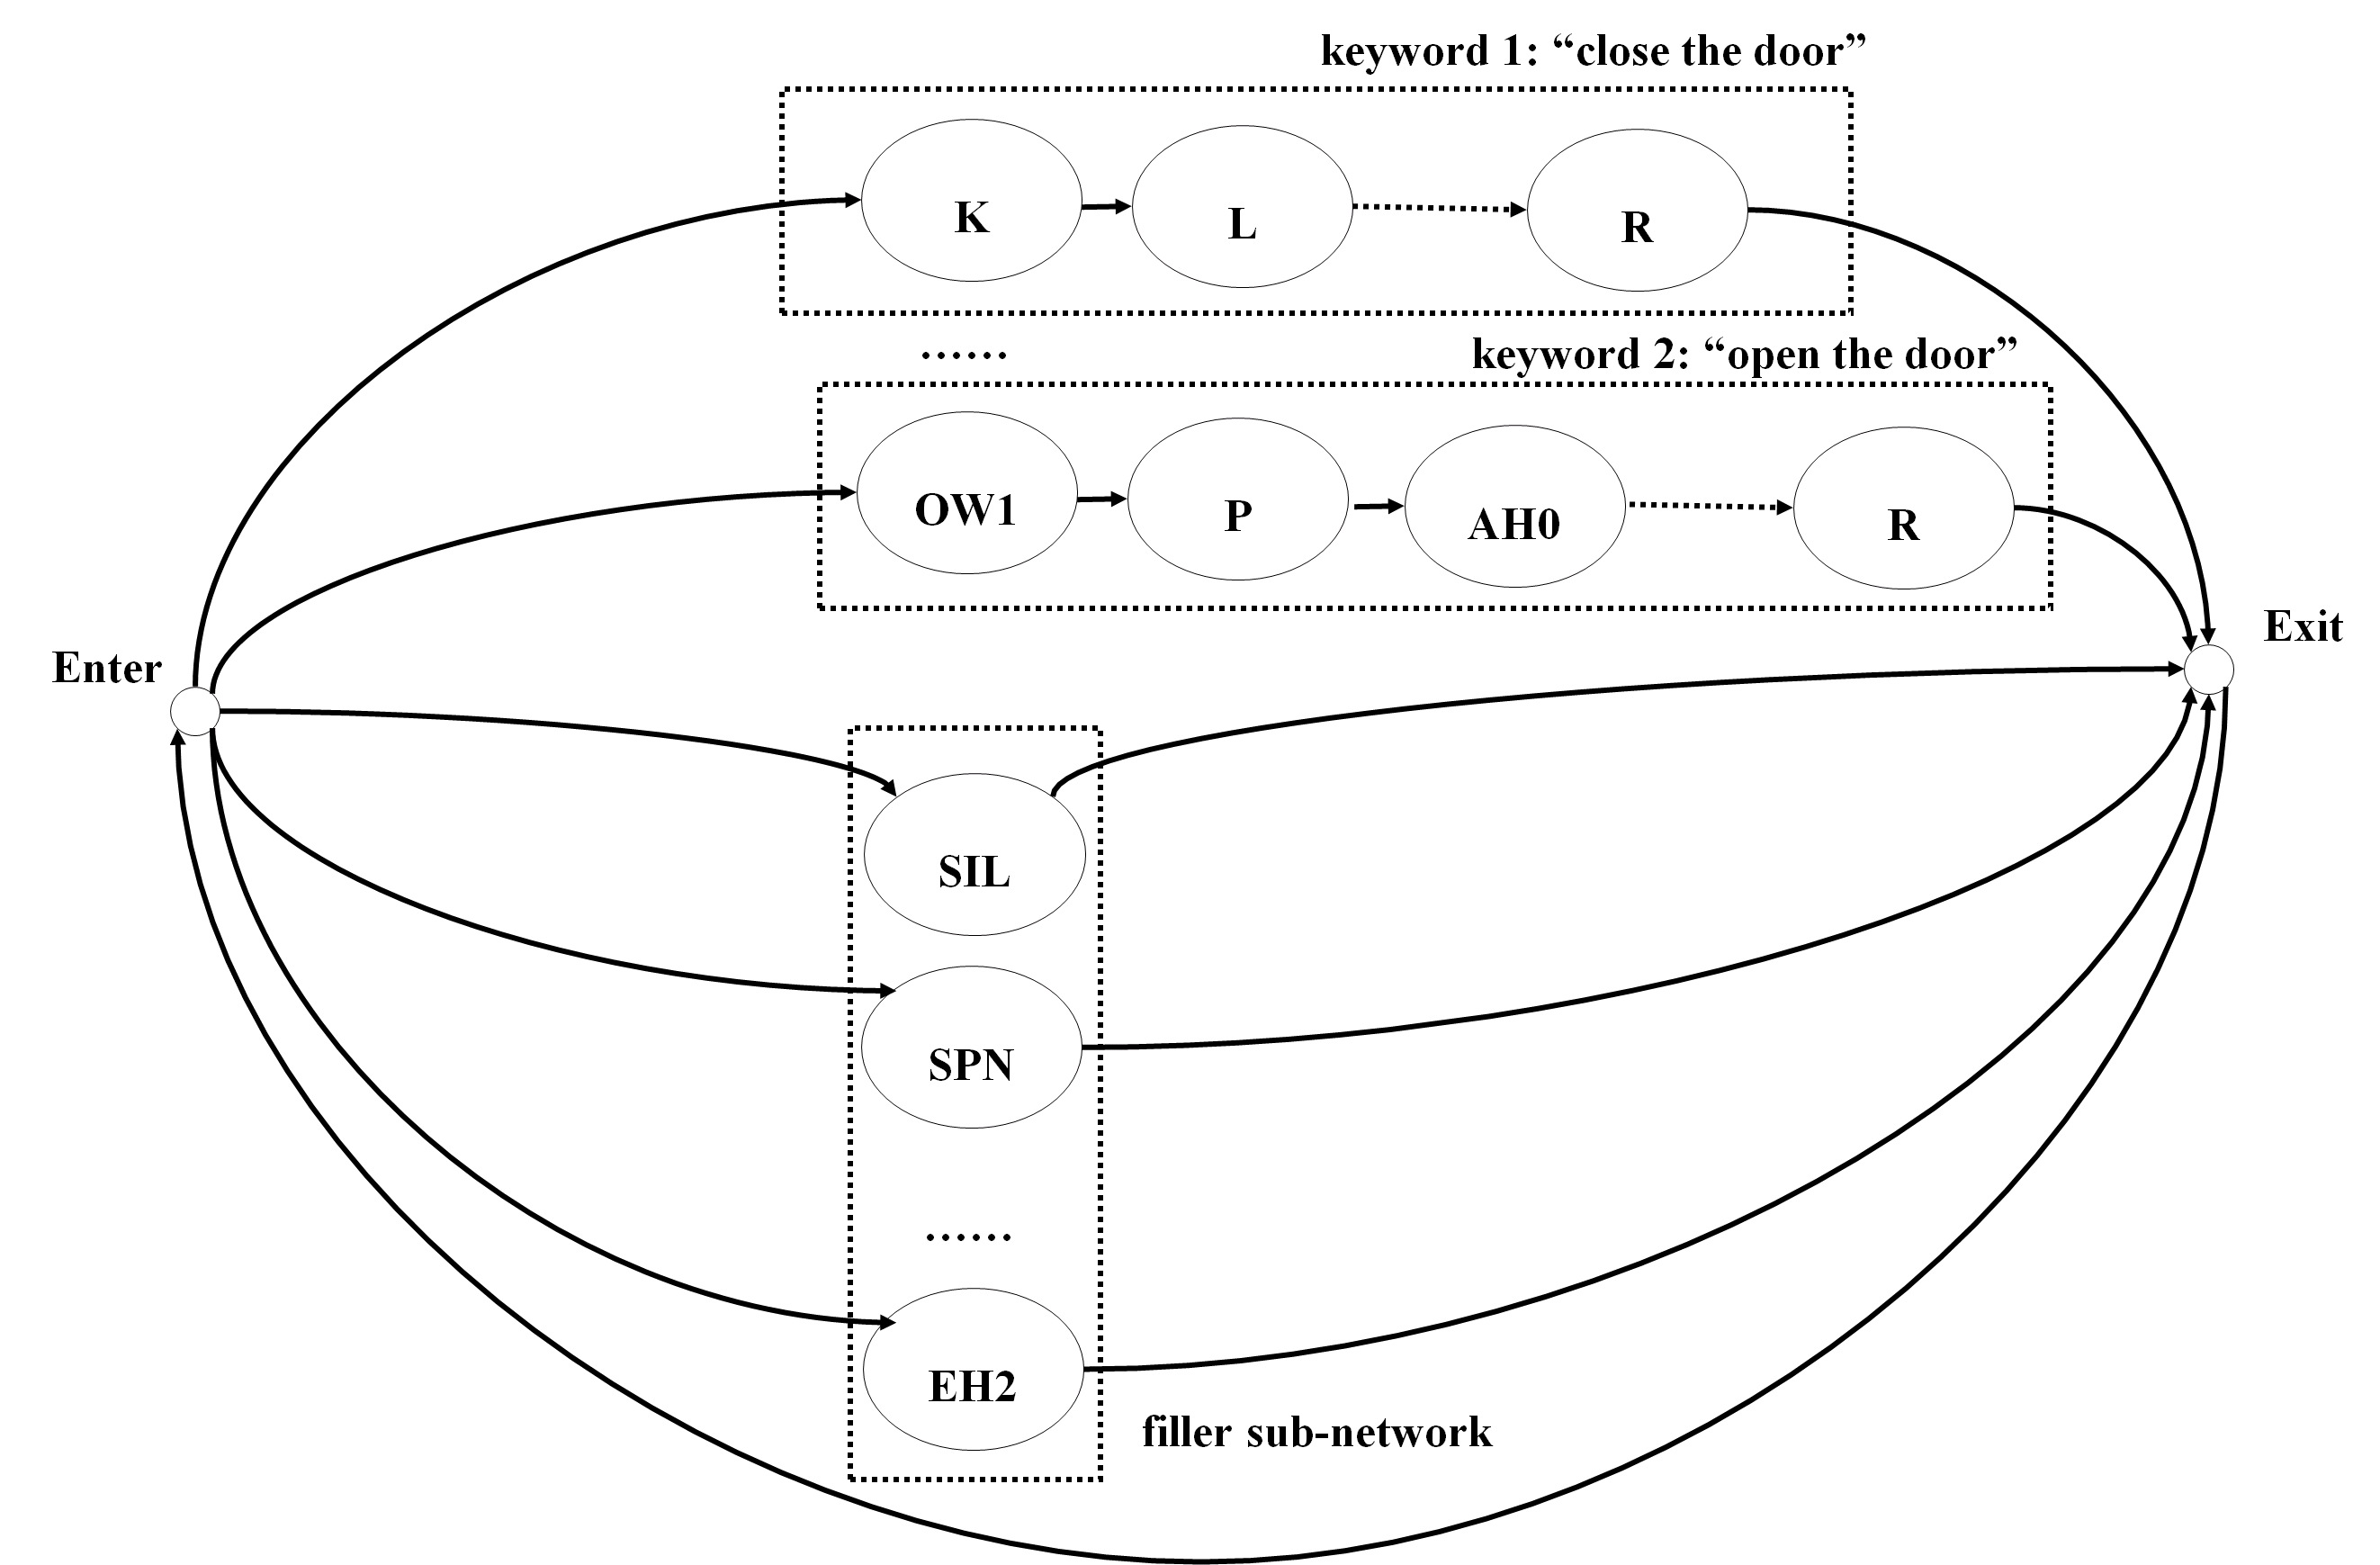
\includegraphics[width=\linewidth]{figure/filler-graph.png}
    \caption{\it 基于 $\tt filler$ 解码的搜索空间结构图}
    \label{fig:filler-graph}
\end{figure}

它包含了两个部分:领域内搜索空间和领域外搜索空间。前者由关键词的子序列建模得到,如图~\ref{fig:filler-graph}中的音素序列。 $\tt filler$ 子网络用于对领域外的搜索空间进行建模。$\tt filler$ 子网络是由所有的音素自环组成的。

\section{基于CTC的关键词检测的标签同步解码}
\label{Sec:kws-ctc}

\subsection{模型训练}
\label{Sec:modeltrain}

如前面章节\ref{Sec:sdm-sdt-intro}所述,序列鉴别性训练的关键之处是竞争序列的建模。
%criteria \& model unit
在本文中,我们研究了两种方向:词语建模和音素建模的CTC关键词检测模型。

为了更好地建模词级CTC模型的竞争序列,这里针对非关键词引入了新的建模单元。
类似于传统的声学KWS方法,代表非关键词的$\tt filler$被引入。在训练阶段, $\tt filler$ 则取代所有标注中的非关键词。

%word boundary modelling
另一个方向是针对音素级模型,我们进行修改的动机是:
i) 任何音素序列,也包括非关键部分,都可以由音素模型来进行建模。
ii) 使得声学模型容易做到与关键词无关,应用于非固定关键词的关键词检测任务。
%
除此之外,我们在词语边界处引入了 $\tt wb$ 单元~\cite{zhuang-is2016}。 在 音素 CTC 中 $\tt wb$ 和 $\tt blank$ 被分别作为词和音素的边界进行建模。区分这样的边界区段不仅可以改善泛化能力,而且也对后面将介绍的后处理有帮助。

这里针对引入的建模单元,公式修改如下:
\begin{equation}
\label{equ:ctc-kw}
\begin{split}
P(\mathbf{L}_u|\mathbf{O}_u)=P(\mathbf{L}_u'|\mathbf{O}_u)_{\mathbf{L}_u' = \mathcal{D}(\mathbf{L}_u)}
\end{split}
\end{equation}
$\mathcal{D}$ 是标签的映射函数。 $\mathcal{D}$ 针对词级或者音素级CTC具有不同的定义。
\begin{equation}
\label{equ:ctc-d}
\begin{split}
\mathcal{D}_{\tt{word}}:\mathbb{L}  \mapsto \mathbb{L}  \cup \{{\tt filler}\}\\
\mathcal{D}_{\tt{sub-word}}:\mathbb{L}  \mapsto \mathbb{L}  \cup \{{\tt wb}\}
\end{split}
\end{equation}
经过修改之后,在词级或者音素级建模中,搜索空间都将包含关键词,非关键词,音素边界和词边界。

\subsection{后处理}
\label{Sec:post-process-ctc}

我们进一步基于最小编辑距离(MED)提出了一个针对CTC推理搜索分布的后处理方法,以便引入音素的混淆性先验知识,增强模型性能。这项工作受到\cite{chaudhari2007improvements}启发, 这里基于CTC词图和MED算法~\cite{7736093}l来针对音素引入混淆建模。 

%which generates a sub-word lattice on the basis of the output probability distribution of CTC and then performs search.  
图~\ref{fig:med-framework} 给出了在音素CTC中使用MED算法的框架。再一句音频中,关键词出现于CTC词图的概率是用三种编辑距离的概率相乘得到的,它们包括插入,删除,替换。每一种操作的概率由MED算法决定。现实中,每个音素在CTC的建模中性能可能各不相同,因此需要进一步采用音素的先验来设计每个音素的阈值,这部分可以通过预先统计得到~\cite{zhuang-is2016}。

\begin{figure}[htbp!]
\centering
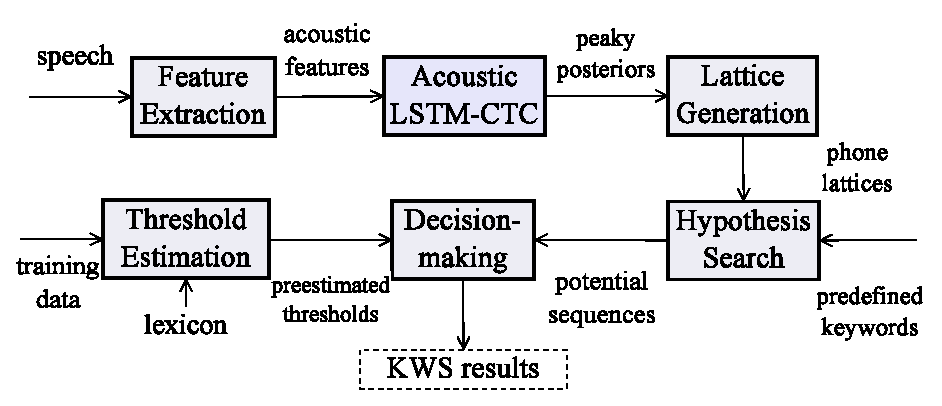
\includegraphics[width=\linewidth]{figure/kws-framework.eps}
\caption{\it 所提出的MED方法的框架。这里使用音素CTC作为例子}
\label{fig:med-framework}
\end{figure}

\subsection{序列鉴别性训练在HMM和CTC框架中的比较}
\label{Sec:disc-and-ctc}

本文中, 序列鉴别性训练被分为两种序列模型而进行: 生成式序列模型 和 鉴别式序列模型。在开始实验部分之前,我们先对两种做法进行一些综合比较:

\begin{itemize}
  \item {\em 生成和鉴别式序列模型}。 在HMM中,需要采用贝叶斯公式将序列状态转移概率和深度学习所估计的后验概率结合起来。在CTC中,给定特征序列后的标签序列的后验概率则直接由深度学习模型进行建模。
  \item {\em 序列建模}。 通过引入 $\tt{blank}$ 到每一帧分解后的建模当中,CTC隐性地对标签进行了序列建模。在HMM中,标签序列被显性地被N元语言模型进行限制和共同建模。
  在计算序列的后验概率时,两种框架都使用了前后向算法。
  \item {\em 混淆区段}. $\tt{blank}$ 原先是提供给CTC进行两个标签之间的混淆区段的建模的。类似的结构也可以如图~\ref{fig:hmm-topo}(c-e)所示在HMM中使用。除了拓扑结构的不同, $\tt blank$ 的粒度在HMM和 CTC中也是初始不同的。
  \item {\em 竞争序列建模}. 在词级CTC中,非关键词元素显示地由建模单元进行建模,即 $\tt filler$ 和 $\tt wb$。 在HMM中,我们采用音素单元对这些竞争序列进行隐性的建模。同时一个音素级的语言模型给出了音素搜索空间的建模效果。 %phone+explicit lm prior
  %\item {\em Discriminative training}. CTC directly models the sequence level posterior probability. The sequence discrimination is implied in the model. For GSM, 序列鉴别性训练 employs maximum a posteriori (MAP) criterion. The discrimination between the correct label sequence and competing hypotheses is modeled by the occupancy probability of the former versus that of the latter.
\end{itemize}

\section{实验结果}
\label{chap:kws-exp}

实验将分别在HMM和CTC框架下进行,我们对两种框架分别进行了序列鉴别性训练实验。
非固定关键词的关键词检测 (语料库检索 任务), 和固定关键词的关键词检测(唤醒词识别 任务)都在实验部分进行了考察。所有实验都是在声学KWS上进行。

%\subsection{非固定关键词的关键词检测 task}
%\label{Sec:}
\subsection{英文语料库检索任务}
\label{Sec:exp-sp-docu-detri}

\subsubsection{实验配置}
\label{Sec:exp-sp-docu-detri-setup}

Wall Street Journal (WSJ0)数据集的一个说话人独立的5k词表数据集 \cite{garofalo1993continous} 被用于评估基于 CTC词图的KWS。 至少出现过5词的词或短语被随机挑选出来作为关键词。总计有50个关键词。

由于WSJ0数据集比较小,同时关键词出现次数较少,因此我们在HMM和CTC中都使用音素作为建模单元,以提高泛化能力,而词作为建模单元将在下章中进行。
输出的音素由CMU 发音词典得到。24维对数filter-bank系数及其第一和第二阶导数组成了10ms固定帧率的特征序列。
HMM模型的配置与 \cite{povey2016purely}中相似,但使用了更好的参数如表~\ref{tab:model-discri} 和表 \ref{tab:perf-all}所示。 我们估计了三元的音素语言模型用于LF-MMI的训练。
%zhc00@qingdao:/aifs/users/zhc00/works/lfmmi/wsj/sjtu$ fstinfo exp/chain/tdnn_sjtu_mono_2n_mhmm1c.NSN.0.1.32.12_nd/phone_lm.fst
我们使用$\alpha=2.5$ 和 $\beta=2.5$ 作为 NU-LF-bMMI的参数。
CTC模型的配置详见 \cite{7736093}。我们使用单向 每层384节点的两层LSTM 进行实验,其带有 128 个节点的映射层。
%The LSTM network was initiated using cross-entropy criterion and then trained using CTC criterion.
%For performance comparison, conventional {\em keyword-filler} DNN-HMM was also trained as baselines. DNN has an 11-frame context window with 5 extended frames on the left and right. %Both HMM systems have 1689 clustered triphone states. 
所有声学模型都使用 Kaldi进行训练~\cite{povey2011kaldi}.
 {\em 等错误率} (EER) 用来度量上面两种测试下的错误率,该指标反映了无唤醒和未唤醒错误的均值。越低的EER表示越好的模型性能。
我们也绘出了receiver operating characteristic (ROC) 曲线,以总结实验结果。
在基于$\tt filler$ 的解码中, 表示为 {\em{kw-filler}}, 而EER是由扫描修改filler权重而得到的。
后验概率平滑,表示为 {\em{smooth}}, 和 CTC MED后处理方法, 表示为 {\em{MED}}, 都是通过\cite{7736093}中提出的固定阈值方法得到的。
\begin{equation}
\label{equ:eer-thres}
\begin{split}
\mathcal T_{EER}(\mathbf{k})=\mathcal T_0+\mathcal T(\mathbf{k})
\end{split}
\end{equation}
公式中 $\mathcal T(\mathbf{k})$ 是针对关键词 $\mathbf{k}$的阈值估计。 $\mathcal T_0$ 在所有关键词中共享,并通过调节它得到EER结果。

{\em 实时率} (RTF), 解码时间与音频时长的百分比, 被作为对整体速度的衡量指标。越低的RTF表示速度越好。
在测试阶段,我们使用的CPU型号为
{\em{Intel(R) Xeon(R) CPU E5-2690 v2 @ 3.00 GHz}}. 
%The ASR decoder used in kw-filler systems is an internal optimized WFST decoder. 
%Clustered cross-word tri-phone HMMs were used as baselines\footnote{Since the KWS task in this paper concerns unrestricted keyword vocabulary, keyword-specific approaches such as \cite{chen2014small} are not appropriate baselines.}.
%A GMM system with 40 Gaussian mixtures and a DNN system of 4 hidden layers with 512 nodes per layer were built.
%The acoustic feature for GMM is 13-dimensional cepstral mean normalized MFCC coefficients  with their first and second order derivatives.

\subsubsection{HMM和CTC模型训练}
\label{Sec:exp-model-arch}
\begin{itemize}
\item {生成式序列模型}
\end{itemize}

本章节比较了不同的声学模型配置。基于HMM的序列鉴别性训练结果见表~\ref{tab:model-discri}。
%model unit (context), hmm topo, MTL. 
这里的所有模型都是通过公式 (\ref{equ:kws-mmi})中的LF-MMI模型进行训练得到的,同时这里使用了KW-Filler的后处理方法。 
\begin{table}[thbp!]
  \caption{\label{tab:model-discri} {\it 基于HMM的序列鉴别性训练的模型框架}}
  %\vspace{1mm}
  \centerline{
    \begin{tabular}{c | c | c |c |c||c}
      \hline
      \multicolumn{1}{c|}{NN Model} &
      \multicolumn{1}{c|}{Context } &
      \multicolumn{1}{c|}{\# Param.} &
      \multicolumn{1}{c|}{CEW} &
      \multicolumn{1}{c||}{HMM} &
      \multicolumn{1}{c}{EER} \\
      \hline \hline
      \multirow{1}{0.1\columnwidth}{BLSTM}&\multirow{1}{0.05\columnwidth}{CD}& 0.60M & 0.1& \multirow{1}{0.05\columnwidth}{PB} & 3.3  
       \\
      \hline
      \hline
      \multirow{7}{0.1\columnwidth}{\textbf{TDNN}}&\multirow{1}{0.05\columnwidth}{CD} & 0.54M& 0.1&\multirow{1}{0.05\columnwidth}{PB}  & 3.3  
       \\
      \cline{2-6}
      &\multirow{6}{0.05\columnwidth}{\textbf{CI}}& \multirow{6}{0.1\columnwidth}{\textbf{0.51M}} & 0.1&\multirow{4}{0.05\columnwidth}{PB}  & 3.3  \\
      \cline{4-4}\cline{6-6}
      &&& 0.4&  & 3.2  \\
      \cline{4-4}\cline{6-6}
      &&&\textbf{0.7}& & 3.1  \\
      \cline{4-4}\cline{6-6}
      &&&1.0&& 3.2  \\
      \cline{4-5}\cline{6-6}
      &&&\multirow{2}{0.04\columnwidth}{0.7} &\multirow{1}{0.05\columnwidth}{\textbf{BP}}  & 3.0  \\
      \cline{5-5}\cline{6-6}
      &&&&\multirow{1}{0.05\columnwidth}{BPB}  & 3.0  \\
      \hline
    \end{tabular}
  }
\end{table}

我们首先对深度学习模型的架构进行了研究。第一二行比较了双向 LSTM (BLSTM) 和 时延神经网络(TDNN)在同等参数下的性能。 BLSTM 包含两层前后向各80个节点的LSTM网络。映射层包含30个节点。 CD TDNN 包含7层100个节点, CI TDNN 包含7层150个节点。结果显示了相似的EER性能。我们相信这是由于: i) 在KWS中,作为模型推理搜索所需要的上下文并不需要很长,TDNN已经足够来针对这样的应用。 ii) 由于KWS模型的参数较少,因此限制了BLSTM模型的性能。在接下来的实验中,我们只讨论TDNN,原因是同等性能情况下它的速度更快~\footnote{我们暂未比较LSTM。近期的一些研究发现TDNN和LSTM可以被结合并取得更好的性能~\cite{tdnnlstm}}。
其次, 模型的建模单元在第二和三行中进行了比较。 tri-phone状态模型, 表示为上下文相关系统 (CD), 与单音素状态模型,表示为上下文无关系统 (CI)进行了比较。
CD模型基于三状态的从左到右的triphone 模型,包括 1536个绑定状态 (senones). 
%zhc00@qingdao:/aifs/users/zhc00/works/lfmmi/wsj/sjtu$ nnet3-info exp/nnet3/nnet_tdnn_a_tiny_smbr/final.mdl
它们的性能接近于 CI 模型。 %Besides the reason previously discussed, the stronger sequence level modeling effect in LF-MMI is another fold~\cite{povey2016purely}. 
第三,对于交叉熵规范化权重,表示为 CEW, 在第三到第六行中进行了调整。
结果显示 $0.7$ 可以得到最优结果,该值被使用在了后续的实验中。该值比LVCSR中偏大,原因是音素语言模型在测试阶段并不存在,这与LVCSR不同,因此训练过程仍在鉴别性训练和交叉熵准则之间权衡。
最终我们使用的拓扑结构如图~\ref{fig:hmm-topo} 
%
所示在第五,七和八行进行了比较。我们提出的BP,BPB比PB\cite{povey2016purely}轻微改善。 
但是在50个关键词上的显著性检验显示结果并不充分 ($\alpha=0.05$, $p=0.18$)。 
性能改善的原因可能为标签延迟所带来的改善~\cite{amodei2015deep},但需要后续更多的研究。 
%And the reason of the similar performance between BP and BPB is also that the label delay makes the confusion span of model inference,  B, mainly exist  before the label output, while the duration of certain pronunciation in the model unit is modeled by the self-loop in the label output HMM state,  P. 
由于BP的搜索空间比 BPB 小,而性能相似,因此后续实验使用BP。

\begin{table}[thbp!]
  \caption{\label{tab:criteria-discri} {\it 基于HMM的鉴别性训练的准则比较}}
  %\vspace{1mm}
  \centerline{
    \begin{tabular}{c ||c}
      \hline
      \multicolumn{1}{c||}{鉴别性训练准则 } &
      \multicolumn{1}{c}{EER} \\
      \hline \hline
%      CE& 4.0 \\
%      \hline\hline
%      CE+sMBR & 3.5 \\
%      \hline
      LF-MMI &3.0 \\
      \textbf{LF-bMMI} &2.9 \\
      LF-sMBR &2.9 \\
      \hline\hline
      NU-LF-bMMI &2.7 \\
      \hline
    \end{tabular} 
  }
\end{table}
第~\ref{Sec:lfmmi-train}章给出了不同准则,在表~\ref{tab:criteria-discri}中进行了比较。 % criteria: CE, mmi, b-mmi, smbr, NU-mmi. 
%The setup is as previously discussed, and 
这里使用 kw-filler进行后处理。 LF-bMMI 和 LF-sMBR 都显示好于 LF-MMI的性能,这与 LVCSR中的结论一致~\cite{vesely2013sequence}. 由于 LF-bMMI 训练快于 LF-sMBR 而性能相似,因此它被用在了后续实验中。
除此之外,NU-LF-bMMI 也参与了比较。这是一个固定关键词的关键词检测算法。在这种情况下,50个预先定义的关键词在训练阶段进行了使用,以加强关键词相关的梯度权重。经过训练之后,声学模型与关键词相关。
NU-LF-bMMI 带来额外的性能提升,而另一方面传统的固定关键词的关键词检测方法~\cite{chen2014small}并不能泛化这样的关键词无关训练集。后续NU-LF-bMMI 并不继续参与该数据集的比较,因为它与关键词无关算法并不可比。

%all tdnn CI kw-filler

\begin{itemize}
\item {鉴别式序列模型}
\end{itemize} 

在音素CTC中,引入的$\tt wb$ 建模单元在表~\ref{tab:wb}中进行了比较。对于少于6个音素的关键词被认为是短关键词,其余的为长关键词。因此可以将关键词集分成两部分分别检查他们的模型性能。
在短和长关键词中$\tt wb$都可以带来性能提升。长关键词的性能一致地优于短关键词,原因是短关键词的音素序列更可能是其他关键词的子集,造成了混淆和误唤醒率;$\tt wb$的引入缓解了这个问题。

 \begin{table}[h]
 \caption{\label{tab:wb} {\it 音素CTC在是否包含 $\tt wb$ 时的模型性能}}
  \centerline
  {
\begin{tabular}{cc||c}
\hline 
Keyword Length & wb & EER \tabularnewline
\hline 
\hline 
\multirow{2}*{short} & $\times$ & 9.0 \tabularnewline
& $\bm{\surd}$ & 4.5 \tabularnewline
\hline\hline
\multirow{2}*{long} & $\times$ & 3.1 \tabularnewline
 & $\bm{\surd}$ & 1.8 \tabularnewline
\hline 
\end{tabular}
 }
%\vspace{2mm}
\end{table}

\subsubsection{后处理和速度分析}
\label{Sec:exp-post-process}

不同的针对HMM和CTC的后处理算法在本节中进行了检查。值得注意的是,本部分是非固定关键词的关键词检测任务,因此音素被用来构建关键词序列。

\begin{table}[thbp!]
  \caption{\label{tab:post-discri} {\it  序列鉴别性训练系统的后处理}}
  %\vspace{1mm}
  \centerline{
    \begin{tabular}{c |c||cc}
      \hline
      \multicolumn{1}{c|}{Model (Crit.) } &
      \multicolumn{1}{c||}{Post} &
      \multicolumn{1}{c}{EER} &
      \multicolumn{1}{c}{RTF}\\
      \hline \hline
      HMM&  smooth &9.8&0.008 \\
      (LF-bMMI)& \textbf{kw-filler} &2.9&0.028\\
      \hline\hline
      %\multirow{2}{0.2\columnwidth}{NU-LF-bMMI}& smooth& 8.5  \\
      %& kw-filler&2.7\\
      %\hline\hline
      %0.026+0.012
       & smooth& 11.4  &0.026\\
     CTC & \textbf{kw-filler}&3.2&0.038\\
      & MED & 3.6 &0.031\\
      \hline
    \end{tabular}
  }
\end{table}
如表~\ref{tab:post-discri} 所示,在 LF-bMMI 和 CTC中,后验概率平滑方法会得到比 kw-filler显著差的结果。但是由于它的速度优势,该方法可以作为实际的前处理,滤除一些容易判断的样本,以减少语料库检索同的计算量。
在 CTC中我们比较了所提出的 MED 算法。
它显示了明显比kw-filler更差一些的性能,但效率较高。该方法将会在后续章节中进一步检验。
kw-filler系统可以使用前述的标签同步解码算法进行进一步速度优化,因此 CTC 可以得到比LF-bMMI更快的速度。最终系统CTC比LF-bMMI慢则源于其使用的LSTM速度比TDNN在LF-bMMI中的使用更慢。

\subsubsection{性能比较}
\label{Sec:exp-perf-comp}

最后,我们将性能和速度的比较总结在表~\ref{tab:perf-all}中。 同时我们绘制出了 ROC 曲线如图~\ref{fig:roc}, 其中越低的曲线结果越好。
其中所有的系统都使用kw-filler作为后处理方法。

\begin{table}[thbp!]
  \caption{\label{tab:perf-all} {\it  非固定关键词的关键词检测中的性能和速度比较}}
  %\vspace{1mm}
  \centerline{
    \begin{tabular}{c | c | c |c ||cc}
      \hline
      \multicolumn{1}{c|}{Model } &
      \multicolumn{1}{c|}{Context } &
      \multicolumn{1}{c|}{\# Param. } &
      \multicolumn{1}{c||}{Criterion} &
%      \multicolumn{1}{c||}{Post} &
      \multicolumn{1}{c}{EER} &
      \multicolumn{1}{c}{RTF} \\
      \hline \hline
      %\multirow{1}{0.05\columnwidth}{dnn}&\multirow{1}{0.05\columnwidth}{CD}&\multirow{1}{0.05\columnwidth}{2.0M}& CE & kw-filler & 5.1 & 0.074 \\
      %\hline
     &\multirow{1}{0.05\columnwidth}{CD}&\multirow{1}{0.05\columnwidth}{0.6M}& CE &  4.0 & 0.051 \\
      %0.015+0.036
      %\cline{2-7}
      %&\multirow{1}{0.05\columnwidth}{CI}&\multirow{1}{0.05\columnwidth}{0.5M}& CE & smooth & 10.2 & - \\
      %\hline \hline
       {TDNN HMM }&\multirow{1}{0.05\columnwidth}{CD}&\multirow{1}{0.05\columnwidth}{0.6M}& CE+sMBR & 3.5 & 0.050
       \\
       %0.015+0.036
       %\cline{2-7}
      &\multirow{1}{0.05\columnwidth}{CI}&\multirow{1}{0.05\columnwidth}{0.5M}& LF-bMMI &  \textbf{2.9} & \textbf{0.028}
       \\
       %0.008+0.020
       %\cline{4-7}
      %&&& NU-LF-bMMI & kw-filler & 2.7 & - \\
       \hline\hline
       \multirow{1}{*}{LSTM CTC}&\multirow{1}{0.05\columnwidth}{CI}&\multirow{1}{0.05\columnwidth}{0.8M}& CTC & \textbf{3.2} & \textbf{0.038} \\
      \hline
    \end{tabular}
  }
\end{table}

\begin{figure}
  \centering
    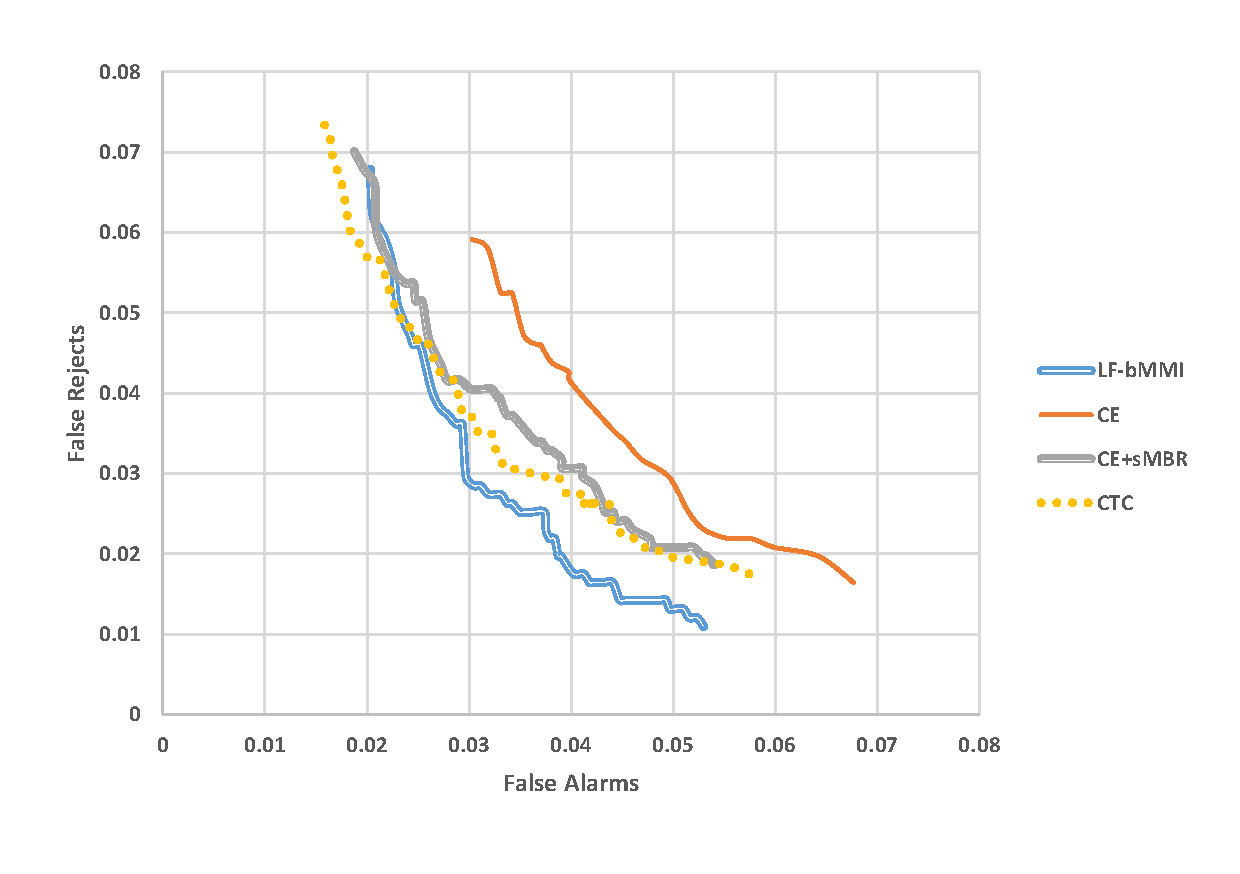
\includegraphics[width=\linewidth]{figure/roc.pdf}
    \caption{\it 非固定关键词的关键词检测的ROC 曲线比较}
    \label{fig:roc}
\end{figure}

这里我们使用交叉熵训练得到的系统作为第一行的基线。它是一个基于 NN-HMM 的传统系统,包含了聚类的tri-phone 状态建模。 这里的HMM拓扑结构见图~\ref{fig:hmm-topo}(a)。
传统鉴别性训练在交叉熵系统基础上进行。这里的词图由模型与一元语言模型解码得到~\cite{povey2007evaluation}。
前两行显示传统的词图鉴别性训练改善了 12\%性能,这一结论与LVCSR中类似~\cite{povey2005discriminative}。 在RTF上的轻微改善则是由于更好的声学模型提供了更少的搜索混淆性。

第三行对比第二行显示了所提出的最好的基于HMM的序列鉴别性训练方法与传统鉴别性训练方法的比较。
%Result shows two folds of superiority
这里显示出 17\% 相对改善 ($\alpha = 0.05$, $p = 0.06$, 在显著性检验测试中) 相比传统鉴别性训练和 28\% 相对改善 ($\alpha = 0.05$, $p = 10^{-5}$)  相比交叉熵训练系统。
这来源于更好的在所提出方法中的建模效果:
\begin{itemize}
 \item 如前文所述,修改后的HMM结构和更低的帧率都能带来性能的改善。
 \item KWS模型的LVCSR词图并不包含较好的竞争路径。这些词图来自声学模型与语言模型的共同解码,而KWS的声学模型性能较弱,并不是针对ASR识别进行设计的。因此这些质量更差的词图限制了鉴别性训练所带来的提升。
 \item 传统鉴别性训练在生成词图时候使用的词级别语言模型在KWS的测试阶段并不存在。而LF-MMI中使用的词级别语言模型则是对于测试阶段使用的由词典构成的关键词序列的一个很好的近似。
\end{itemize}
除此之外,与CE基线相比,LF-bMMI 系统取得了一倍的加速,原因在于模型推理搜索和解码搜索都得到了加速。对于前者,主要是由于帧率减少。而后者主要是由于所使用的CI单元比传统CD单元少,使得搜索空间变少,这也包括对filler模型的相应简化。

使用LSTM的CTC系统在最后一行中,也显示了比传统CE模型更好的性能 ($\alpha = 0.05$, $p = 0.01$) 以及比传统鉴别性训练系统更好的性能 ($\alpha = 0.05$, $p = 0.11$)。 从图~\ref{fig:roc}中看, CTC系统存在相对较多误唤醒。

我们在一些初始的尝试中使用基于HMM的序列鉴别性训练作用在CTC初始化的变种模型上~\cite{sak2015fast,nict-icassp17}。但结果并不成功,没有带来改善: 在词级别CTC中~\cite{li2018developing}, LVCSR 解码词图不包含有效的竞争路径 。而在音素级别模型上,如前所述,词图的质量限制了传统框架下鉴别性训练所能得到的改善。% ii) Essentially, after CTC pre-training, the state prior probability $P(\mathbf{L})$~\cite{nict-icassp17} is combined with the original model to form a CTC variant. The CTC variant models $P(\mathbf{O}|\mathbf{L})$, and become a GSM. 

\subsection{中文数据集唤醒词识别}
\label{Sec:exp-wakeup-word-rec}
\subsubsection{实验配置}
\label{Sec:exp-wakeup-word-rec-setup}
%data
%20170321 bj123 定制唤醒词 baseline.txt
本章节进一步测试了在固定关键词的KWS系统中的性能。我们准备了一个类似于文献\cite{chen2014small}和  \cite{cas-icassp17}中介绍的数据集。它包含两部分:通用语音数据和关键词相关数据集。第一部分包含100小时,第二部分包含30K关键词正例,和180K关键词负例。详细的数据集配置可以参见~\cite{chen2018kws}。

%metrics
测试数据包含两部分:关键词相关集合和环境噪声集合。第一部分用于测试模型在区分关键词和非关键词时候的能力\cite{chen2014small}。 它们包含2K正例和10K负例,代表了 20\% 左右的比值,这符合该应用的实际应用场景。前文我们讨论的EER被作为准则。
环境噪声集合则用于测试模型对误唤醒的鲁棒性\cite{cas-icassp17}。它包含300小时的环境噪声。每小时的误唤醒次数记为 {\em{误唤醒频率}} (FAF), 也被作为度量模型性能的指标。
后处理中获取EER的超参数方法如前面章节所述。
每个关键词都单独包含它自己专门的平滑方法的阈值。总体的EER是每个关键词EER的平均值。
之后我们会固定所有的超参数并测试系统在噪声集合中的FAF。

%model 
在该任务中,我们测试了词级系统和音素级系统。HMM和CTC的鉴别性训练系统与传统交叉熵系统进行了比较。词级系统的输出为关键词序列中的每个词,而音素级系统的输出则为中文中的不带调音节。特征和声学模型配置与前面章节一致。
NU-LF-bMMI采用$\alpha=10.0$ 和 $\beta=10.0$。

\subsubsection{实验结果和比较}
\label{Sec:exp-wakeup-word-rec-result}

表~\ref{tab:perf-mandarin}显示了相应的结果。
一个交叉熵训练的词级别的TDNN系统被作为基线系统~\cite{chen2014small}。该系统采用了后验平滑作为后处理方式。

%compare EER \& FAF

\begin{table}[thbp!]
  \caption{\label{tab:perf-mandarin} {\it  固定关键词的KWS系统的性能和速度比较}}
  %\vspace{1mm}
  \centerline{
    \begin{tabular}{c|m{4.5em}|c|c||ccc}
      \hline
      %&
      %&&& \multicolumn{4}{c}{post-processing} \\
      %\cline{4-7}
      %&
      %&&&  \multicolumn{2}{c}{smooth} & \multicolumn{2}{c}{kw-filler} %& \multicolumn{2}{c}{MED}\\
      %\cline{4-7}
      \multicolumn{1}{c|}{Model}
      &\multicolumn{1}{c|}{Unit} 
      &\multicolumn{1}{c|}{Criterion}&\multicolumn{1}{c||}{Post }&EER&FAF&RTF%&FS&RTF
      \\
      \hline\hline
      %/aifs/users/zhc00/works/kws/lfmmi_chn700/exp/nnet3/chn700.subsetby20_train.nnet_tdnn_a_tiny/
      \cite{chen2014small}
      &\multirow{1}{*}{Word}
      &CE &smooth & 6.2 & 0.64 &0.014\\
      %0.013
     \hline\hline
      %
      \multirow{3}{*}{HMM}&\multirow{3}{*}{Syllable}
      &CE & & 10.2 & 1.40 &0.041\\
      %0.015+0.026
      %\cline{3-7}
      %/aifs/users/zhc00/works/kws/lfmmi_chn700/exp/chain/.tdnn_sjtu_mono_2n_mhmm1c.0.1.128.4_nd.chn700/
      && LF-bMMI &kw-filler &8.3& 1.06 &0.033\\
      %0.008+0.025
      %\cline{3-7}
      %/aifs/users/zhc00/works/kws/lfmmi_chn700/exp/chain/res_a.0.99.tdnn_sjtu_mono_2n_mhmm1c.0.1.128.4_nd.chn700/decode_testset.full.lnovopc_mcsnor_evl17feb_v1_graph_res3/scoring_kaldi/kws.rst2
      %exp/chain/chn700.subsetby5_train.res_a.0.99.tdnn_sjtu_mono_2n_mhmm1c.0.1.128.4_nd.chn700/decode_testset.full.lnovopc_mcsnor_evl17feb_v1_graph_res3/scoring_kaldi/kws.rst2
      && NU-LF-bMMI& & \textbf{5.2} &\textbf{0.51} &\textbf{0.029}\\
      %0.008+0.021
      \hline\hline
      %/aifs/users/zhc00/works/kws/ctc_chn700/ctc
      \multirow{2}{*}{CTC}
      &\multirow{1}{*}{Word}
      & \multirow{2}{*}{CTC} &smooth &9.1 & 1.13 & 0.024  \\
      %\cline{2-2}\cline{4-7}
      %ref: https://spetechcular.com/trac/asr/wiki/ctc_kws_chn_car https://spetechcular.com/trac/asr/wiki/%E6%AF%85%E8%90%8C2016#a2016.6.6
      &\ +{\tt filler}& &MED & \textbf{7.0}&\textbf{0.90} & \textbf{0.029}\\
      %0.024
      \hline
    \end{tabular}
  }
\end{table}

在第二行中,模型也是通过CE准则进行训练的。模型的建模单元是音节,后处理方法为 kw-filler。 
该系统性能在EER和FAF中都有所下降,原因是音素级系统具有更多建模单元。而这些建模单元都被等同地进行训练。与之相反,词级系统则可以对特定关键词具有更强的建模能力。
\cite{chen2014small}中显示了类似结论,这说明后验概率平滑方法的CE模型系统是一个较强的基线系统。

在第三行中,我们所提出的LF-bMMI系统显著改善了CE系统,取得了一致更优的EER和FAF。但是,所得到的系统仍然差于基线系统。为了解决针对关键词区段识别性能差的问题,我们使用了NU-LF-bMMI 方法,在第四行中。结果显示NU-LF-bMMI 系统得到了相对第一行基线中显著更好的结果。我们认为这包括两方面原因:第一,非一致地训练关键词相关的音素序列,理论上等同于对关键词的每个词单元专门进行训练,所以其建模能力类似; 第二,由于音素系统通过所提出的NU-LF-bMMI增强了关键词之间与关键词和非关键词之间的鉴别能力,因此它能够取得更优的性能。关于效率,虽然该系统的模型推理搜索速度较快,但由于引入kw-filler的搜索部分,因此导致两倍的速度减慢。使用标签同步解码算法对系统进行加速是未来一个值得研究的问题。

最终,CTC系统也参与了比较。在第五行中的系统类似于\cite{fernandez2007application}。虽然它在文献\cite{fernandez2007application}中取得了较好的性能, 但在本部分测试中仍然差于词级别的CE系统。我们相信这是因为我们使用的训练和测试集相比该文献具有更大的挑战。我们针对这一系统如前文所述,添加了 $\tt filler$ 建模单元,以改善关键词与非关键词之间的鉴别性;同时我们增加了基于 MED的后处理算法,以便引入音素混淆性的先验知识。我们所提出的系统在第六行中取得了显著更好的结果。但是这个系统仍然没有超过传统的CE系统。
%This may be because the baseline in fixed vocabulary KWS is highly tuned while the CTC-MED approach treats all phones equally during training. It is worth noting that due to the same reason, the LF-bMMI approach does not outperform the baseline neither. 
我们认为进一步的改善应该包括两方面:对CTC模型的噪声鲁棒性的研究;使用更好的深度学习模型来改善模型性能。
%in keyword specific corpus 

%MED uses


\section{本章小结}
\label{chap:kws-sum}

本章节提出了基于序列鉴别性训练的深度学习关键词检测模型的训练框架。通过使用音素语言模型或者使用显性添加建模单元的方式,对竞争可能路径进行建模,由此得到更好和更快的序列鉴别性训练。
我们的实验在语料库检索任务和唤醒词识别任务上进行。对于前者,词表大小通常是无限制的,而对于后者,则要求有更强的噪声鲁棒性。相比于传统的逐帧CE深度学习模型在固定关键词和非固定关键词的关键词检测任务上的最好的系统,尽管不同应用具有不同的特征,但是实验显示我们所提出的鉴别性训练方案可以取得一致和显著的改善。


\chapter{基于GPU并行计算的搜索速度优化}
\label{chap:gpu}

本章节中我们将着重介绍我们针对Kaldi开源工具包的一个扩展,以便使它能够支持图形处理芯片(GPU)上的WFST解码推理搜索。该框架可以显著加速现有推理搜索算法,特别是在基于深度序列学习的一系列模型上进行了验证。

我们将维特比算法中的令牌合并操作实现为一个GPU并行计算中的原子操作,以便减少维特比束剪枝算法中的同步开销;我们提出了动态负载均衡的方式以更高效地进行并行计算,提高其多线程之间的利用率;我们重新设计了基于GPU并行计算的精确的词图生成和剪枝算法,以便充分利用GPU的性能特点。

在Switchboard 上实验表明,我们所提出的方法在取得完全一致的1-best和词图质量情况下,可以得到3-15倍的加速,并在绝大部分GPU架构上进行了验证。除此之外,如果再进行多句子的并行处理,最终的加速比将达到46倍。


\section{引言}
\label{chap:gpu-intro}

近来深度学习语音识别的发展唤起了大量语音识别转录的需求。在这一系统中,计算量较大的部分主要包括:声学模型推理和语言模型WFST解码。

为了减少声学模型推理的计算开销,研究人员们提出了一系列效率更高的声学模型,包括一些比较新颖的神经网络结构~\cite{xue2014singular,peddinti2018low}, 定点化
~\cite{mcgraw2016personalized}, 跳帧~\cite{pundak2016lower,zhc00-chen-is16,zhc00-chen-tasl2017}
和端到端系统~\cite{audhkhasi2017direct,e2e-2018}.
%frame sub-sample or PSD, novel model, SVD, quantization, ...
同时算法的改进,比如剪枝~\cite{mohri2002weighted,hori2004fast}
和向前预测~\cite{soltau2009dynamic,nolden2012search}是针对解码部分主要的加速方式。
%in WFST framework, pruning , lookahead ... in e2e framework...

如第~\ref{chap:intro2-dec-todo}章节中对于解码搜索的研究机遇的讨论,
基于GPU的并行计算是另一种潜在的针对语音识别计算的加速方式。针对声学模型推理,由于大部分计算量集中在矩阵形式的运算,因此它易于通过将类似于训练过程中\cite{vesely2010parallel}的序列批处理~\cite{dixon2009harnessing} 引入推理搜索阶段,以加速运算。
但是,基于GPU并行计算的WFST解码并不容易实现。尽管一些研究在小型语言模型上取得了一定成功~\cite{you2009parallel},但这些系统仍然受制于两部分缺陷:i) 由于GPU显存有限,这些方法并不能有效利用较大的商用语言模型。
ii) 这些方法并不通用,常常受制于特定的声学或语言模型,并且没有词图生成功能。 %Detailed comparisons are in
%Section~\ref{sec:relate}. 
%is another ... , show  potential to allow  speech processing ...  and can be applied on all above model or algorithm side trials.
%to speedup the first part.  batching
% second part insufficient, 
%especially in the context of deep Learning, 
%lack of lattice processing; 
%hard to utilize large LM
%


这项工作作为Kaldi工具包的一个扩展~\cite{povey2011kaldi},实现了基于GPU并行计算的WFST解码。
%
这是一个通用的离线解码器~\footnote{近期的研究显示,使用CPU比较容易得到一个实时的解码器来针对在线解码应用
 ~\cite{peddinti2018low,zhc00-chen-tasl2017} 。因此我们的目标集中在如何解码海量的离线语音,降低其计算损耗。},
 该解码器对语言模型和声学模型没有特别的限制,并且可以工作在各种架构的GPU上。
%
为了支持第二遍重打分和更丰富的后处理,我们的设计基于WFST解码和词图生成的架构~\cite{povey2012generating}。
%
我们对这项工作进行了开源~\footnote{\url{https://github.com/chenzhehuai/kaldi/tree/gpu-decoder}},
它将会与大多数Kaldi脚本相兼容。


\section{维特比算法并行化框架}
\label{chap:gpu-viterbi}

我们所提出的系统工作在二遍解码框架下~\cite{woodland19951994},以便能够支持更大的语言模型,并支持词图上丰富的后处理。

\subsection{系统框架}
\begin{figure*}[ht]
  \centering
    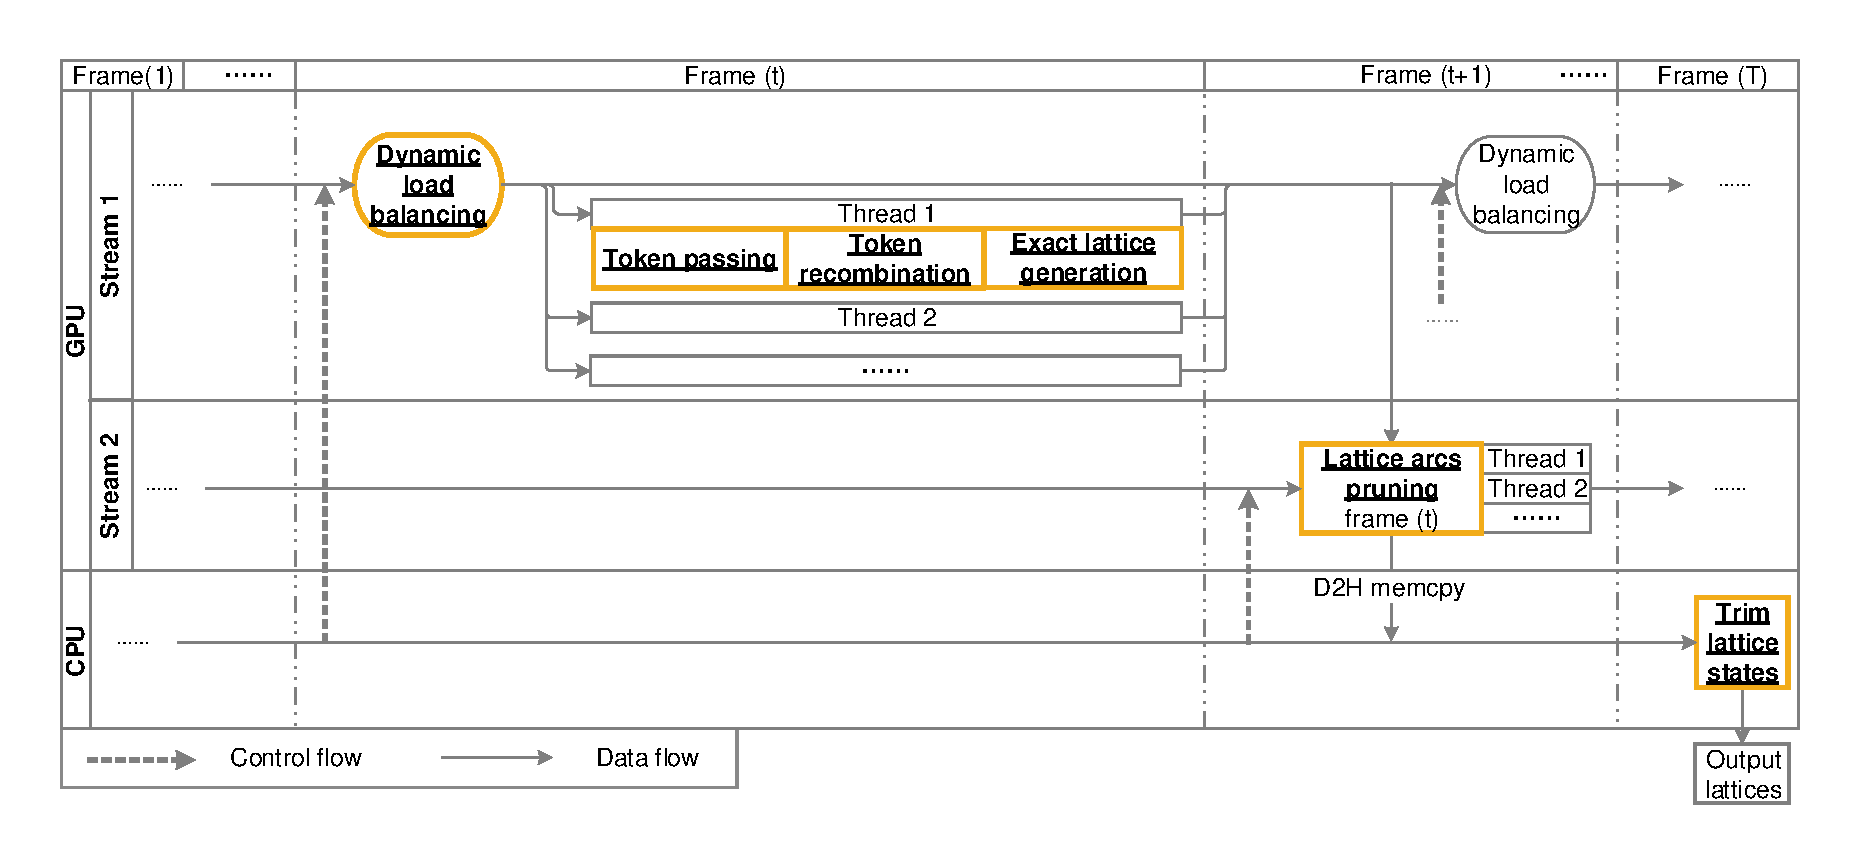
\includegraphics[width=1\linewidth]{figure/gpu_framework.pdf}
    \caption{\it  并行维特比束剪枝算法以及精确词图处理系统的框架}
    \label{fig:gpu-framework}
\end{figure*}
图~\ref{fig:gpu-framework} 显示了系统的框架,这包括两个GPU同时处理流,分别进行解码和词图剪枝,它们完全并行同时受不同CPU线程所控制。具体来说,对第 ($t+1$)帧, 第二个处理流将处理第一个流产生的第($t$)帧的词图。
%GPU and CPU work asynchronously and there are two GPU concurrent streams
%performing decoding and lattice processing respectively.

解码的流程类似于CPU 版本~\cite{povey2011kaldi},但工作在不同的一些设计上,以适应并行计算需求,其罗列于下面的章节。负载均衡算法则处理了线程之间并行的分配,它们具体体现在如何分配WFST状态和边。
%position of 4 topics below in the system and acts like an overall procedure/algorithm




\section{并行的令牌传递算法}
\label{sec:atomic}

下面我们首先介绍维特比搜索中将会引入的同步时间开销,它具体出现在令牌合并过程中。
%
% Take Hidden Markov Model (HMM) as an example.  It is defined
% as the conditional likelihood $p(\mathbf{O}|\mathbf{L})$ of a feature sequence ${\mathbf O}$ given a label sequence $\mathbf L$.
% \vspace{-2em}
% \begin{eqnarray}
% \label{equ:hmm-model}
% %\begin{split}
% p(\mathbf{O}|\mathbf{L})
% %&=&\!\!\!\!\!\!\sum_{\mathbf{q}\in\mathcal{A}(\mathbf{L})}\!\!\!p(\mathbf{O},\mathbf{q}|{\mathbf L}) =\sum_{\mathbf{q}}\prod_{t=1}^{T} p({\bf o}_{t}|q_t) P(q_t|q_{t-1})\nonumber\\
% %y_{ut}(s^{(r)}_{ut})
% &\propto&\sum_{\mathbf{q} \in\mathcal{A}(\mathbf{L})}\prod_{t=1}^{T} \frac{P(q_t|{\bf o}_{t})}{P(q_t)}P(q_t|q_{t-1})\\
% %\end{split}
% \label{equ:hmm-model-viterbi}
% &\propto&\max_{\mathbf{q}}\prod_{t=1}^{T} \frac{P(q_t|{\bf o}_{t})}{P(q_t)}P(q_t|q_{t-1})
% \end{eqnarray}
% %\end{split}
% where $\mathbf{L}$ is a label sequence, and
% $\mathbf{q}$ is a HMM state sequence and  $q_t$ is the HMM state at frame $t$. $P(q_t|q_{t-1})$ is the HMM state transition probability and $P(q_t)$ is the state prior probability of $q_t$.  The posteriors $P(q_t|{\bf o}_{t})$ are estimated using neural networks (HMM-DNN).
% $\mathcal{A}$ is a mapping function from  $\mathbf{L}$ to its corresponding HMM
% state sequence $\mathbf{q}$. In Viterbi algorithm, the sum over $\mathbf{q}$ in
% Equation~\eqref{equ:hmm-model} is replaced by the best state sequence as shown
% in Equation~\eqref{equ:hmm-model-viterbi}.
%
% An alternative formulation of the Viterbi algorithm is used in ASR, called Token Passing algorithm~\cite{woodland19951994}.
% %
在ASR解码中,维特比搜索被实现为 \textit{令牌传递算法}~\cite{woodland19951994}, 其令牌表示的是截止 $t$帧情况下的一个局部识别序列,同时对于每一个 WFST状态在 $t$帧时都可以用一个可移动的令牌进行表示。
在每一帧,维特比路径是通过 \textit{令牌合并}过程得到的, 其他一个 \textit{min} 操作被加到了每个状态的所有输入边上 (比如对状态7,在图~\ref{fig:load-balance} 中,那么它的输入边包括2至7,5至7,7至7三条), 这里我们需要计算得到它们之中的最佳分数,以及这个分数来自哪一个状态。

%Thus for a state, tokens coming from different paths need to be compared and recombined together in serial. 
%Only the best one is passed to the next WFST state,
%and describe in CPU how to do it.
%
%and it is the bottleneck of parallel methods. 


\begin{algorithm}[ht]
%\vspace{-0.25em}
\caption{线程级别的令牌合并算法 \textcolor[rgb]{0,0.5,0}{(Inputs: accumulated cost, an out-going WFST arc and a current token)}}
\label{code:atomic}
\begin{algorithmic}[1]
\Procedure{Recombine} {cost, arc, curTok}
\State oldTokPack = state2tokPack[arc.next\_state]
\State curTokPack = \textit{packFunc}(cost,arc.id) \Comment \textcolor[rgb]{0,0.5,0}{pack into uint64}
\State ret = \textit{atomicMin}~\footnotemark(oldTokPack,curTokPack)
\If { ret $>$ curTokPack }         \Comment \textcolor[rgb]{0,0.5,0}{recombine}
\State  perArcTokBuf[arc.id] = *curTok \Comment \textcolor[rgb]{0,0.5,0}{store token}
%\State  modified[arcId] = 1
\EndIf
\EndProcedure
%\\
%\textcolor[rgb]{0,0,0}{[A grid barrier before the next procedure]}
%\Procedure{Tok. Storage} {curTokPack, toToken}
%\State arc = \text{unpackFunc}(curTokPack).arc  \Comment \textcolor[rgb]{0.8,0,0}{ back to int32}
%\State *toToken = *perArcTokBuf[arc] \Comment \textcolor[rgb]{0.8,0,0}{recombine stage 2}
%\EndProcedure
\end{algorithmic}
\end{algorithm}
\footnotetext{\textit{atomicMin}({\em{*address}}, {\em{val}})~\cite{cuda9}. Computes \textit{min}({\em{*address}}, {\em{val}}), writes the result to {\em{address}}, and returns the original {\em{*address}} .}

%\textit{atomicMin}(address, val). Read the 64-bit {\em{old}} located at the {\em{address}}, computes the \textit{min} of {\em{old}} and {\em{val}}, and stores the result to {\em{address}}~\cite{cuda9}.}
%\vspace{-1em}

原始的CPU算法在进行令牌合并时候是串行的。我们即将讨论如何在GPU中实现令牌合并,而将如何高效并行这些指令放在下面的章节中。一种最简单的实现是通过添加critical sections~\cite{lamport1979make}
以便使令牌合并这一步仍然恢复串行。这种设计不仅低效,而且会在早期GPU中引入死锁。
\cite{you2009parallel} 提出一种在每个状态上做针对所有令牌传递结果的规约操作,但这样将引入额外的规约过程中的写冲突和同步损耗,而且这些损耗总是发生在计算的最后阶段。
%
\cite{kim2011h} 提出将所有数据编码到32比特上,然后使用GPU原子操作来实现令牌合并。这种方法损失了计算精度,并且使解码算法受制于特定的模型。

我们提出算法~\ref{code:atomic}, 它是一个通用的计算方法,适应于任何模型的令牌合并,没有精度损失。这个算法执行于每一个GPU线程上,并且针对每一条WFST边进行并行,比如在图\ref{fig:load-balance} 中从状态2到状态7的边可以由这一算法进行处理。
% describes the 2-stage atomic operation based token recombination. 
我们首先将分数和边的索引合并为一个64比特整形数,以表示合并之前的令牌, 同时我们将分数放在高位上,使得它可以控制后续的合并结果。在每一帧,我们将所有令牌的信息保存在一个长度为所有可行边的数组上。这保重合并过程没有写入的冲突,也就不会带来同步损耗。所有的令牌都被处理后,我们收集所有仍然活跃的合并令牌,将64比特数字返回原先的分数和边的索引,由此将真正的令牌信息存入相应的令牌中,而这一步也同样是并行进行的。


\section{图搜索的动态负载均衡算法}
\label{sec:para-viterbi}

另一个并行算法的问题是负载均衡。
对每一个状态,我们并行地遍历所有它的输出边,直到到达了一个终止节点。由于WFST状态可能具有完全不同的输出边数,如果不能合理地将线程分配给这些边,将导致负载不均问题。
文献\cite{you2009parallel,mendis2016parallelizing}中重新设计了 WFST结构以减少这种不均。不同于这些工作,我们不希望解码算法依赖于特定的声学,词典,语言模型。因此我们依然基于原始的WFST结构。
我们首先提出\textit{静态负载均衡算法}, 它首先对每个线程计算如何分配WFST边才能得到大致相等的数量,经过那之后才开始进行处理。这样的设计引入了额外的并行求取累积和的开销~\footnote{具体来说是一个GPU上的DeviceScan操作,其工作在大约 10K 个整形数上。},
这种方法将引入计算和GPU内核启动的额外时间开销。

受~\cite{alakeel2010}的启发,我们进一步引入了
\textit{动态负载均衡算法},其呈现在算法~\ref{code:load-balance}中。我们使用一个调度中心来分配令牌,同时我们令 $N$个线程为一个组 ($N = 32$) 来共同处理从一个状态(令牌)出发的所有WFST边。当一个令牌的所有边都被处理完毕了,它就会找调度中心取到下一个令牌。我们同时将调度中心实现为一个GPU原子操作。图~\ref{fig:load-balance}显示了其中的一个例子。在实验中我们比较了两种不同的负载均衡算法。


%Algorithm~\ref{code:load-balance} shows dynamic load balancing
\vspace{-0.5em}
\begin{algorithm}[ht]
%\vspace{-0.25em}
\caption{Grid级别的令牌传递算法 \textcolor[rgb]{0,0.5,0}{(N=32; Inputs: the current active token vector)}}
\label{code:load-balance}
\begin{algorithmic}[1]
\Procedure{ Dynamic Load Balancing } {toks}
\State group = cooperative\_groups::tiled\_partition$\left<32\right>$
\If{group.thread\_rank()==0}\Comment\textcolor[rgb]{0,0.5,0}{rank 0 in each group}
\State i = \textit{atomicAdd}(global\_d,1)  \Comment\textcolor[rgb]{0,0.5,0}{allocate new tokens}
\EndIf      %\Comment\textcolor[rgb]{0,0,0}{i=global\_d++}
\State i = group.\textit{shfl}(i,0) \Comment \textcolor[rgb]{0,0.5,0}{rank 0 broadcasts i to whole group}
\If {i$>=$sizeof(toks)} return\Comment \textcolor[rgb]{0,0.5,0}{all tokens processed}
\EndIf 
\For {arc in tok2arcs(toks[i])} \Comment \textcolor[rgb]{0,0.5,0}{thread parallelism}
\State {\bf call} \textit{Recombine}(toks[i].cost+arc.cost, arc, toks[i])
\EndFor
\EndProcedure
\end{algorithmic}
\end{algorithm}


\begin{figure}[ht]
  \centering
    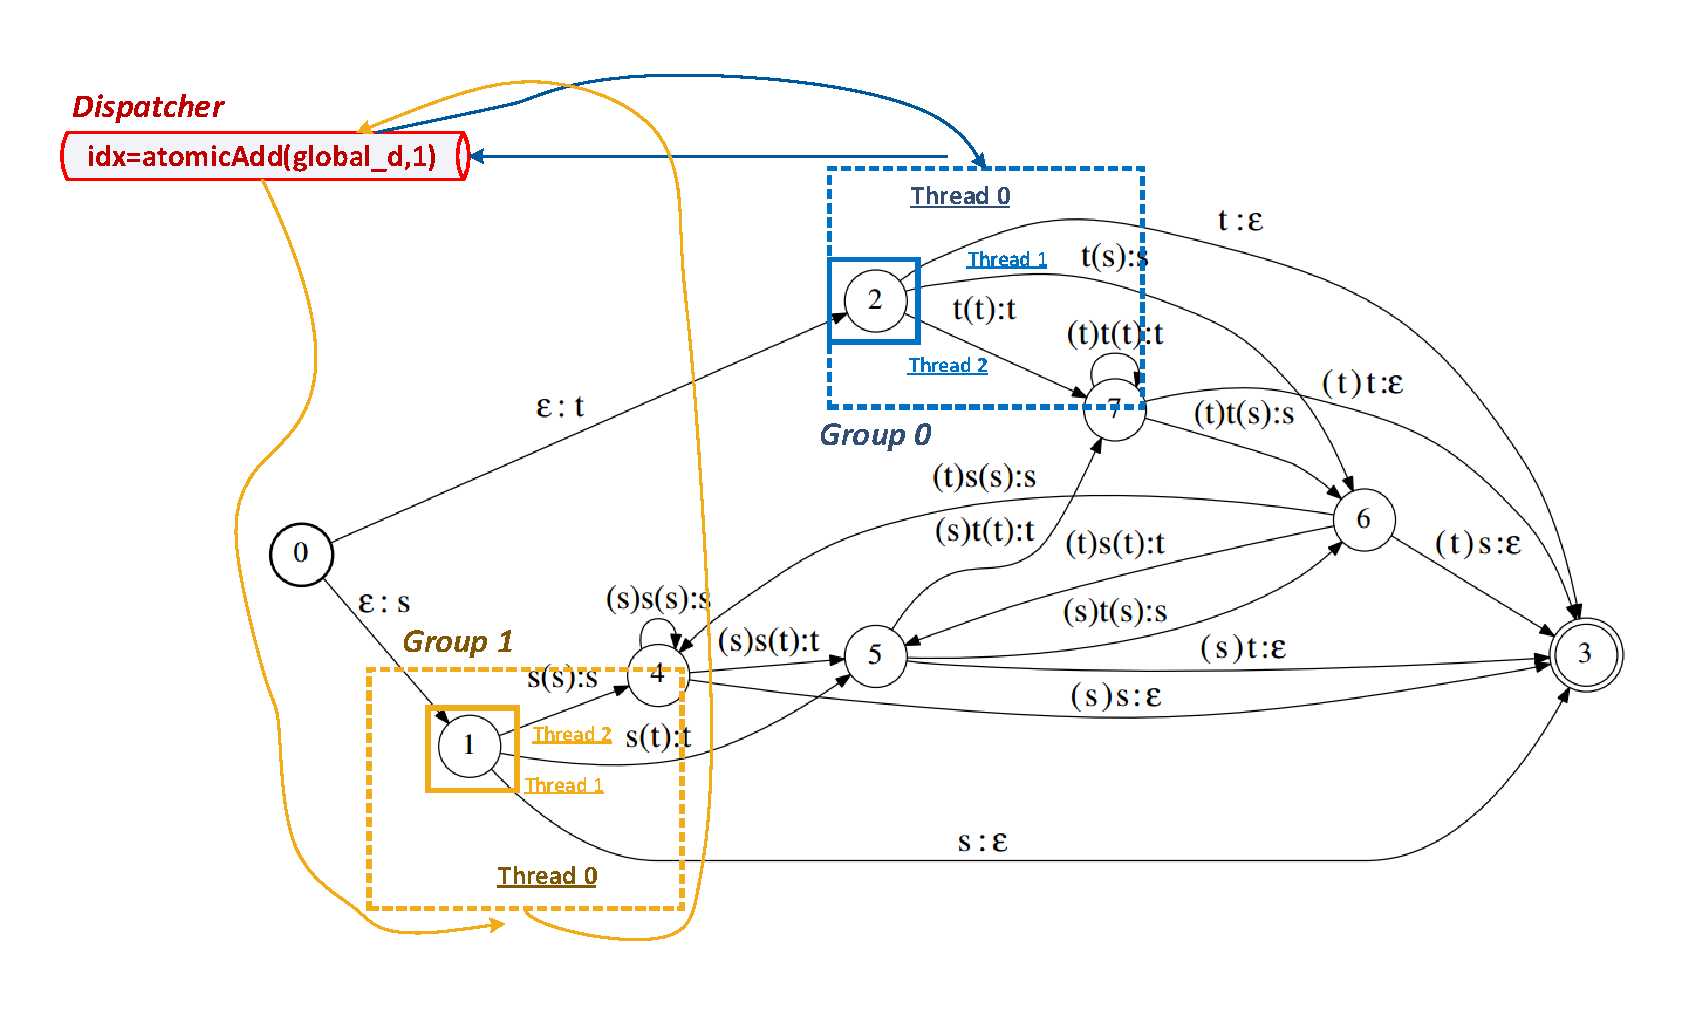
\includegraphics[width=1.1\linewidth]{figure/load-balance.pdf}
    \caption{\it 一个针对动态负载均衡的例子。这里的虚线框表示一个
      CUDA cooperative group ,不同的组分表示为不同的颜色。每一个组由线程0进行控制。当某个组分处理完了从一个状态出发的所有边,线程0将会向调度中心索要下一个令牌,并通知组分里的其他线程。而调度中心使用原子操作来保证每个令牌只分配给一个组分。组0和组1完全工作在并行方式中。}
    \label{fig:load-balance}
\end{figure}

\section{并行的词图处理算法}
\label{sec:lat-gen}


\subsection{精确的词图生成算法}
WFST精确词图~\cite{povey2012generating} 是指在词图上保存了准确的分数和状态级对齐关系,这些信息对于语言模型重打分,丰富的语音识别后处理等都有重要作用。~\footnote{除了本文中研究的置信度应用~\cite{mangu1999finding} ,它同样可以用于加速最小贝叶斯风险解码~\cite{goel2000minimum},
系统融合~\cite{fiscus1997post}, 鉴别性训练~\cite{povey2005discriminative}, 等等。 }。 %We examine lattice rescoring and confidence measure in this paper.
但是在GPU中实现词图处理算法并不简单。
\cite{kim2014accelerating} 提出在GPU中解码,而后在CPU中生成词图,这不仅引入新的同步损耗,使解码器速度下降,而且引入了大量的device-to-host (D2H) 内存拷贝问题。
%(much slower, sec 2.2, fig 2).
我们通过重新设计了一个并行版本的词图处理算法\cite{povey2012generating}更彻底地解决了这个问题。

%enable GPU decoder with large scale LM rescoring (enable GPU decoding in real application).
%ours comparable to no-lat; 

在词图生成中,对每一个令牌传递操作,会有一条词图边被记录到GPU显存中。我们设计了一种GPU向量结构来保存这些边。这种向量实现了  {\em{push\_back}} 算法,其通过原子操作来分配特定内存给相应词图边,而整体内存则被预先分配完毕,增量扩展。

为了减少原子操作所带来的损耗,我们提前分配好 $K$个向量,并随机选取一个向量执行 {\em{push\_back}} 操作。经过令牌传递之后,这些来自$K$ 个向量的边被收集起来。对于词图节点,我们可以使用类似的方案~\footnote{在我们早前的实验中,在 $K=32$时,这一优化可以10倍加速词图边处理的速度。这项加速针对词图节点并不明显。}。



\subsection{词图剪枝}

并行词图剪枝算法基于引文~\cite{ljolje1999efficient,povey2012generating}中方法,并针对GPU并行处理进行了必要的修改。

原始的CPU版本词图剪枝算法会迭代地更新节点和边的额外权重,直到它们停止改变;而额外权重定义为当前边的最佳权重与最佳路径上的权重的差值。对于一些权重过高的边,将会被剪枝,直到一个节点上的所有边都被剪枝。在GPU版本实现中:i) 我们将迭代更新节点和边的过程进行了GPU线程的并行化;
ii) 我们使用一个全局的边向量数组来代替原始实现中的链表结构,原因是链表结构并不能被随意访问(random access),而是总要从头进行访问;
iii) 我们将额外权重迭代更新实现为一个原子操作,以减小同步时间开销。

 当一条词图边被剪枝后,我们不会物理上删除这条边,原因是内存分配时间开销较大。相反,我们在剪枝的最后进行并行收集操作,将所有剩余边一次集中到GPU向量结构中,类似于第~\ref{sec:lat-gen}章中的做法。 这种实现方法的内存开销将会在实验中进行讨论。
%Lattice nodes not associated with remaining arcs are removed in CPU processing for ease of implementation without adding much overhead.
同时,我们没有裁剪词图的节点,原因是:i) 我们需要词图边上能够寻迹到词图节点上,并且在D2H拷贝前后都要有唯一对应,因此我们没有改变节点的相对位置。ii) 在CPU中会重新建立起节点和边的链表关系,因此没有边连接的节点将被隐含删除。 iii)  节点的D2H拷贝是与解码和词图处理异步的,因此不会对最终速度造成影响。

本文提出的词图处理算法总结如下:
 \vspace{-0.25em}
 \begin{algorithm}[ht]
 %\vspace{-0.25em}
 \caption{Grid级别的词图处理算法  \textcolor[rgb]{0,0.5,0}{(Input: processing frame, lattice token vector and lattice arc vector are taken as inputs)}}
 \label{code:exact-lattice}
 \begin{flushleft}
 Function {\em{ArcExtraCost}}(arc) returns the cost difference between the best path including the arc, and the best overall path.
 \end{flushleft}
 \begin{algorithmic}[1]
 \Procedure{ Prune Lattice For Frame } {f, toks, arcs}
 \For{tok in toks(f-1)} \Comment \textcolor[rgb]{0.8,0,0}{extraCost initialization}
 \State tok.extraCost = FLT\_MAX
 \EndFor
  \While{modified == 1}
 \State  modified = 0
 \For{ arc in arcs(f)} \Comment \textcolor[rgb]{0.8,0,0}{thread parallelism }
 \State cost = \textit{ArcExtraCost}(arc)
 \If { cost $<$ latticeBeam}
 \State \textit{atomicMin}(tok.extraCost,cost)
 \State \textit{atomicAdd}(modified,1)
 \EndIf
 \EndFor
 \EndWhile
 \EndProcedure
 \end{algorithmic}
 \end{algorithm}

\section{实验结果}
\label{chap:gpu-exp}

\subsection{实验配置}
在Switchboard 300小时数据集上,
%acoustic model baseline setup~\cite{peddinti2018low}  (one tdnn-lstm-chain and one tdnn-lstm-ce).
我们测试了两个声学模型基线系统:一个是文献 ~\cite{peddinti2018low}中的 ``TDNN-LSTM-C''模型,其使用无词图鉴别性训练准则 (LF-MMI)~\cite{povey2016purely},包含了降帧率技术。
我们同时测试了未降帧率模型,它是一个多层BLSTM模型~\cite{sak2014long},使用交叉熵进行训练。% in Section~\ref{sec:exp-ana}. %For the bidirectional LSTM network, we stack 3 bidirectional LSTM layers together with recurrence interval equals 1, 2 and 3 respectively.

%  \item language model and WFST Decoder~\cite{povey2012generating}
测试是在NIST 2000 CTS集合上进行的。
一个30K词表大小,从Switchboard 数据集标注训练的3元语言模型被用于第一遍解码,与Fisher数据集插值的4元语言模型被用于词图重估打分。Kaldi的1-best解码器和词图解码器被用作CPU解码器的基线系统~\footnote{Kaldi中的{\em{decode-faster-mapped}} 和 {\em{latgen-faster-mapped}} 工具}.

% \vspace{-0.25em}
% \begin{algorithm}[ht]
% %\vspace{-0.25em}
% \caption{Grid-level Lattice Processing  (processing frame, lattice token vector and lattice arc vector are taken as inputs)}
% \label{code:exact-lattice}
% \begin{flushleft}
% Function {\em{ArcExtraCost}}(arc) returns the cost difference between the best path including the arc, and the best overall path.
% \end{flushleft}
% \begin{algorithmic}[1]
% \Procedure{ Prune Lattice For Frame } {f, toks, arcs}
% \For{tok in toks(f-1)} \Comment \textcolor[rgb]{0.8,0,0}{extraCost initialization}
% \State tok.extraCost = FLT\_MAX
% \EndFor
%  \While{modified == 1}
% \State  modified = 0
% \For{ arc in arcs(f)} \Comment \textcolor[rgb]{0.8,0,0}{thread parallelism }
% \State cost = \textit{ArcExtraCost}(arc)
% \If { cost $<$ latticeBeam}
% \State \textit{atomicMin}(tok.extraCost,cost)
% \State \textit{atomicAdd}(modified,1)
% \EndIf
% \EndFor
% \EndWhile
% \EndProcedure
% \end{algorithmic}
% \end{algorithm}
% \vspace{-1em}
%  \item metrics: WER, oracle lattice WER (hard to do in SWBD), rescored WER, NCE result and 

我们对1-best 结果和词图质量都进行了比较。为了公平起见,我们保持两种解码器得出相同的词图密度 ({\em{lat.den.}}, 其使用arcs/frame进行度量)~\cite{woodland19951994}。
在语音识别任务中,我们使用词错误率(WER), 词图重估错误率(lattice rescored WER) ({\em{+rescored}}), 词图最佳错误率 (lattice oracle WER, OWER)~\cite{hoffmeister2006frame}。Normalized cross entropy (NCE)~\cite{siu1999evaluation}被用于评估词图得出的置信度的质量。这里我们训练了决策树以将这些词图后验概率转换为我们最终需要的置信度~\cite{chen2017confidence,chen2017unified}.
实时率 (RTF) 用于度量解码器速度和相应针对CPU基线系统的加速比 ($\Delta$) 。由于本文专注在WFST解码的加速上,因此我们所报道的RTF排除了声学模型的推理搜索所占用的时间。下文中我们会对总体的RTF稍作讨论。由于本文主要考虑快速的离线转录系统,因此时延并未加入比较。所有的实验都是在  {\em{E5-2686 v4 @ 2.30GHz}} 的CPU上进行,其包含 1 socket (8 threads)。 % (see amazon cluster)
一块 Tesla V100 默认地用于GPU解码,后续我们还会比较其他GPU架构下的性能。


\subsection{性能和速度}
\label{sec:speedup}

表~\ref{tab:gpu-perf-compare} 中比较了我们所提出的GPU词图解码器在使用相同beam大小情况下的准确度(性能)比较。
结果中所有的指标都非常接近。在词图结果中的轻微差别来自于词图生成过程中的不同访问次序。
%The parallel token passing changes the 
%sequence of token visiting, which results in  slight differences. 

\begin{table}[thbp!]
  \caption{\label{tab:gpu-perf-compare} {\it  1-best 和词图性能比较 (beam=14).  } }
  \centerline{
    \begin{tabular}{c c || c c c| c}
      \toprule
      %zchen@login:/export/a12/zchen/works/decoder/egs/swbd/s5c$ grep Sum exp/chain/tdnn_lstm_1e_sp/decode_decode.conf.eval2000_sw1_fsh_fg/score_10_0.0/*ctm.filt*sys
      %|  Sum/Avg      |  4459     42989   |  87.7        8.5       3.8       1.8      14.1      49.8   |
      %/export/a12/zchen/works/decoder/egs/mini_librispeech/s5_otf/is2018.sh
      system &  {\em{lat. den.}} &WER & {\em{+rescored}} & OWER & NCE \\
      \midrule
      %/export/a12/zchen/works/decoder/egs/swbd/s5c/get_conf.sh
      %/export/a12/zchen/works/decoder/egs/swbd/s5c/is2018.sh
      %grep Sum exp/chain/tdnn_lstm_1e_sp/decode_decode.conf.eval2000_sw1_fsh_fg//score_*/eval2000_hires.ctm.map.filt.sys
      %| Sum/Avg    | 4459  42989 | 87.5    8.9    3.6    1.9   14.4   50.6 |  0.323 |
      %| Sum/Avg    | 4459  42989 | 87.4    8.6    4.0    1.7   14.3   50.5 |  0.322 |
      CPU  & 30.3  & 15.5 & 14.3 & 11.2& 0.322\\
%\midrule
      %tmp/tdnn_lstm_1e_sp.2/ana/lat.ora.log
       GPU  & 30.2  & 15.5 & 14.3 & 11.2~\footnote{该表中的OWER 是不准确的,因为我们没有进行文本规范化,导致数值偏大。在另一个 LibriSpeech~\cite{povey2016purely}数据集中排除了该问题,我们可以一致地发现CPU和GPU的OWER 都是 23\% 的 WER (3.4 v.s. 14.7) 。  }  & 0.328\\
\bottomrule
    \end{tabular}
  }
\end{table}

解码的实时率和加速比的比较参见表~\ref{tab:speedup}。
%We mainly focus on time of the search process  (explain why), give general RTF in text/footnote with single stream (with multi-stream, the speed could be even faster). Notice that RTF from kaldi log should be divided by 3.
在1-best和词图解码中,我们分别取得了15倍和9.7倍的加速。这里的大部分加速来自于平行处理WFST的节点和边的过程。
%
当我们使用GPU的并行技术MPS时,我们可以得到46倍的序列并行加速比。MPS是一种减小GPU context切换损耗的技术~\cite{cuda9}。
作为对比,我们在CPU上使用了类似的序列并行技术,但仅取得了1.8倍的加速比。
%

虽然原子操作优化的加速比并不明显,它有效去除了critical section,而这部分使得使用传统GPU框架进行解码成为可能,这部分我们将在后文中讨论。同时动态负载均衡取得了最好的实验效果。
%(which metric can be used to show the effect of load balancing)

为了更公证地比较总体的RTF,我们使用一个GPU独立进行单序列声学模型推理。单序列的总体RTF在1-best解码器和词图解码器上分别为 0.18 和 0.03~\footnote{这里的声学模型推理还可以使用序列批处理进行额外加速~\cite{dixon2009harnessing}, 我们以往的经验是有10倍左右的加速比。}。 更深层次地将声学模型推理和语言模型解码相结合,是一个有意义的未来研究课题。

%script/run_swb.1b.sh
%fff6e20f60bf4147cced7a9e498c25e65e79e327
%18fe57790198b64799af7ac51675b0b70ecedac8
\begin{table}[thbp!]
  \caption{\label{tab:speedup} {\it  所提出系统的速度比较 (beam=14). }}
  \centerline{
    \begin{tabular}{ m{11em} || c c| c c}
      \toprule
      system  & \multicolumn{2}{c|}{search} & \multicolumn{2}{c}{ + lattice}  \\
       & RTF& $\Delta$&RTF & $\Delta$  \\
      \midrule
      %exp_dec/latgen_v2a/graph_sw1_tg/log.cpu
      %exp_dec/latgen_v2a/graph_sw1_tg/log.cpu.nl
      CPU    &  {\bf{0.16}}& {\bf{1.0X}} &{\bf{0.27}} & {\bf{1.0X}} \\
      %exp_dec/latgen_v2a/log.cpu.pal
      %kaldi don't have parallel decoding without lattice
      \ \ + 8-sequence (1 socket)~\footnote{The result is obtained from {\em{latgen-faster-mapped-parallel}} in Kaldi. 1-best decoder do not have such implementation. }  & - & - & 0.15 & 1.8X\\
      \midrule
       GPU &  0.016 & 10X &0.080 & 3.3X \\
       \ \ + atomic operation & 0.015  & 11X &0.077 & 3.5X\\
       \ \ \ \ + dyn. load balancing & {\bf{0.011}}  & {\bf{15}}X & 0.075  & 3.6X\\
       %exp_dec/latgen_v2a/graph_sw1_tg/log.gpu
       \ \ \ \ \ \ + lattice prune &  - & - & {\bf{0.028}}& {\bf{9.7}}X\\
       %run_pal.v2.2.sh TOFI
       \ \ \ \ \ \ \ \ + 8-sequence (MPS) & 0.0035   & 46X &  0.0080 & 34X\\
       %moderate
      \bottomrule
    \end{tabular}
  }
\end{table}



\vspace{-0.25em}
\subsection{分析}
\vspace{-0.25em}
\label{sec:exp-ana}

图~\ref{fig:exp-ana} 显示在各种不同的语音识别系统上,该解码器能够取得一致的显著加速。

\begin{itemize} 
   \item GPU 架构比较。
 \end{itemize} 
 该系统可以工作在Kepler之后的GPU架构中。在非常早期的K20 GPU上它仍然取得了3倍相比CPU的加速比。
 \begin{itemize} 
   \item 声学模型帧率
 \end{itemize} 
 我们测试了原始帧率而非降帧率后的声学模型,用图中的虚线表示。它仍然显著比CPU的降帧率系统好。值得注意的是这说明CPU系统比GPu系统慢了3倍以上,因为降帧率技术同样非常重要,可以显著加速解码系统~\cite{pundak2016lower,zhc00-chen-tasl2017}。而这项技术在GPU解码器中仍然很重要。
\begin{itemize}
   \item 语言模型大小和内存开销。
 \end{itemize} 
 这里我们测试了Fisher数据集插值后的4元语言模型,并将它剪枝到不同大小后编译成HCLG~\cite{mohri2002weighted} 进行测试(13MB, 62MB, 196MB, 258MB)。这里的CPU解码器一致性地慢于GPU系统。

 另一方面,我们使用一个11GB WFST在 12GB显存的 TITAN GPU上测试了该GPU解码器。这种大小的WFST基本可以满足商用需要。更多关于内存优化的细节可以参考我们最新发布的开源代码。

 除此之外,我们发现当CPU解码器使用的语言模型大小变化之后,其速度变化相对GPU略微小一些,原因是CPU解码器会进行逐边剪枝;而GPU解码器则是进行统一的剪枝。因此针对GPU解码器的剪枝策略的研究也是未来一个很有意义的课题。


% ; for GPU, always traversal parallel, while K20 computation ability ...; Nevertheless, the corresponding system still speeds up by 3 times

%\vspace{-0.25em}
%\begin{itemize}  
  %\item  shows different language model size, framerate, GPU architectures (need to modify the color style and background)




\begin{figure}
  \centering
    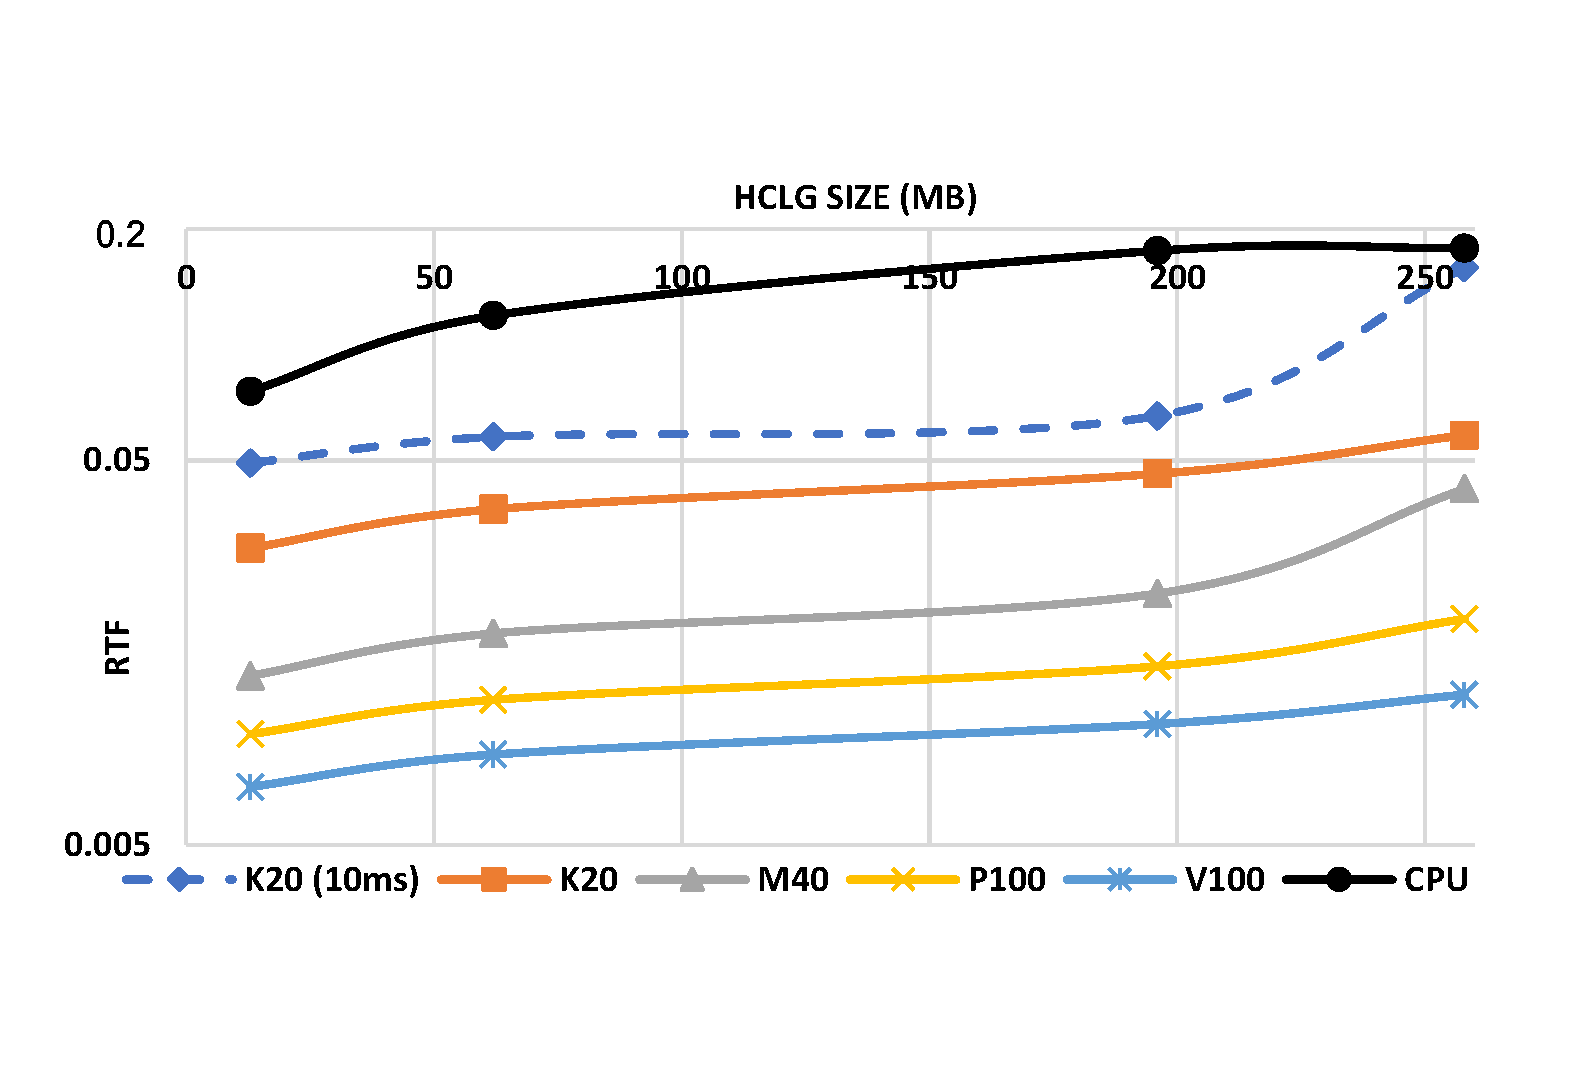
\includegraphics[width=\linewidth]{figure/gpu_analysis.pdf}
    \caption{\it  语言模型大小,帧率,GPU架构的比较}
    \label{fig:exp-ana}
\end{figure}

\begin{itemize} 
   \item Profiling.
   \vspace{-0.25em}
 \end{itemize} 
  图~\ref{fig:exp-profile} 比较了CPU和GPU的各个子模块的时间占用~\footnote{词图生成在CPU中被包含到令牌传递部分中} 。
  % (we can change this one to a histogram figure like this "Exploring Recognition Network Representations for Efficient Speech Inference.pdf", figure 4)
  GPU在显著快于CPU版本的同时,每部分分布比较均衡,显示出系统并没有显著的瓶颈。GPU解码器的令牌传递和词图处理都得到了显著加速。同时 ``other'' 部分包含了GPU的内核启动时间和同步等待时间。对于这些部分的优化也是未来研究的一个有意义话题。

\begin{figure}[ht]
  \centering
    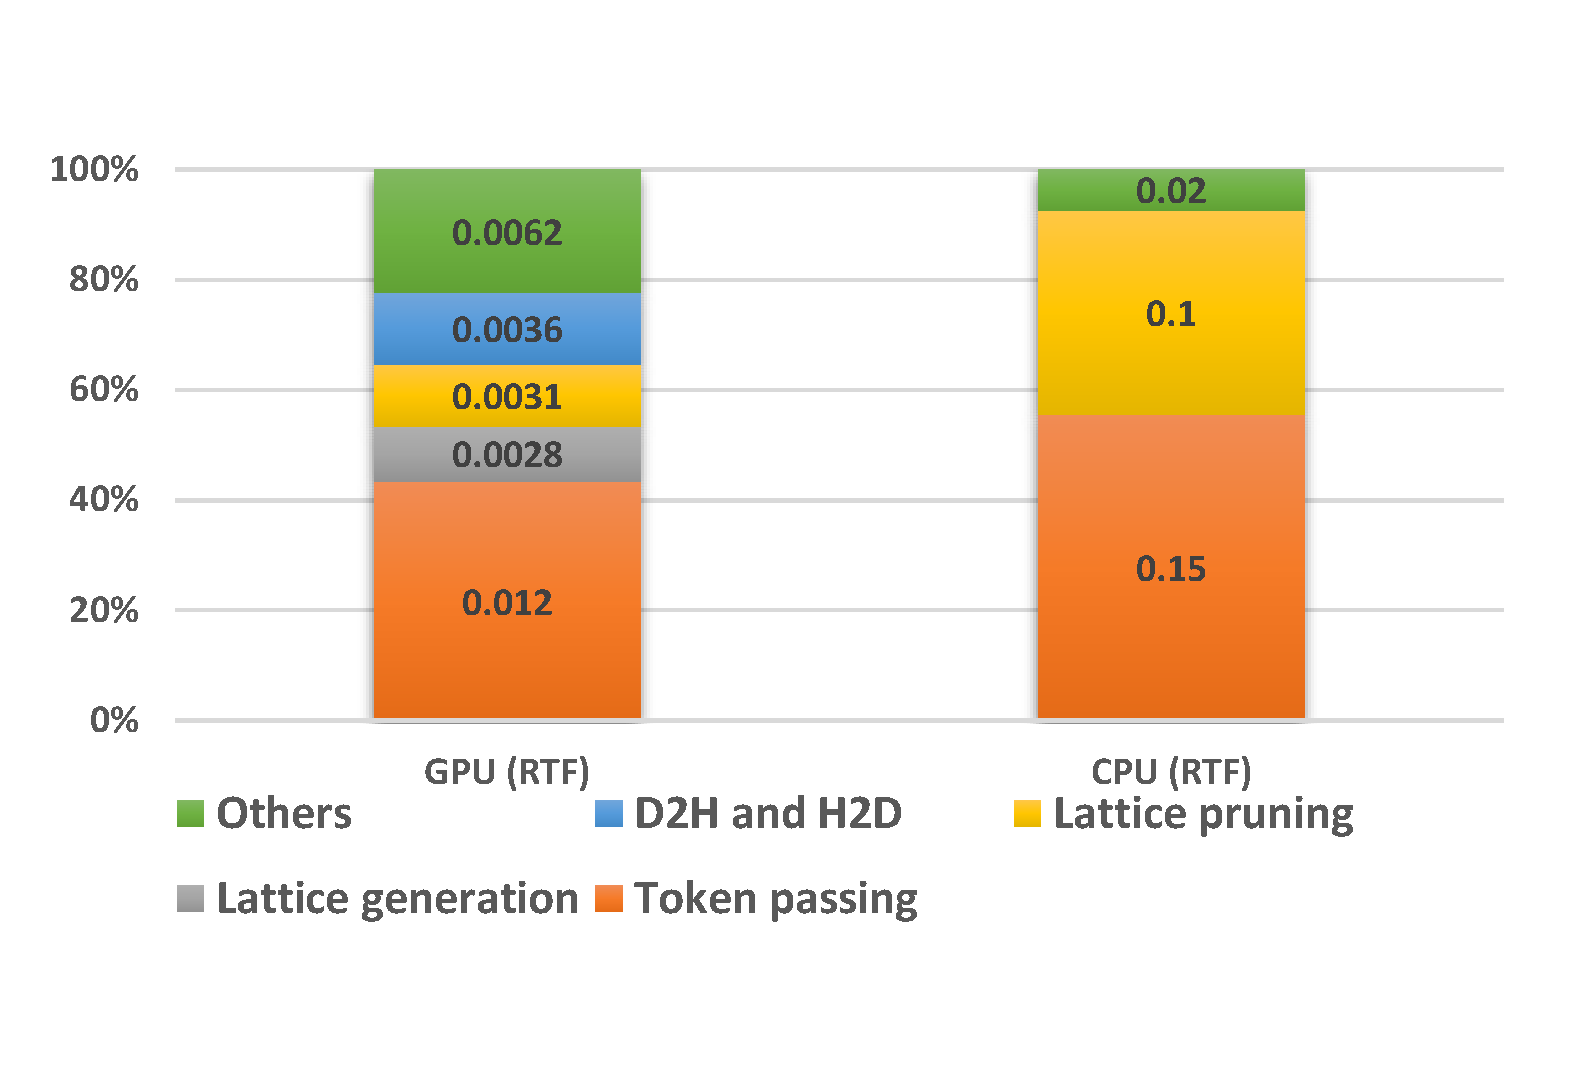
\includegraphics[width=1\linewidth]{figure/gpu_profile.pdf}
    \caption{{\it 针对解码器的时间占比分析} }
    \label{fig:exp-profile}
\end{figure}



\section{本章小结}
\label{chap:gpu-sum}

在这项工作中,我们描述了所提出的基于GPU并行计算的WFST解码器,我们将该实现融合在Kaldi开源工具包中。我们设计了并行版本的解码和词图处理算法。该系统相比CPU版本取得了显著的性能提升,并且该实现可以推广到大部分GPU架构中。最后,我们还将该实现完全开源。


\chapter{基于标签同步解码的搜索空间优化}
\label{chap:lsd}

我们在上一章节中提到,语音识别的速度与分类器推理计算和搜索解码算法两部分相关,而前者易于抽象化为矩阵的并行计算从而得到显著加速,因此一般不构成主要瓶颈。上一章节的工作从并行计算的角度对后者进行了加速,降低了公式(\ref{equ:dec-cmp-dec})中的$\mathbb{C}_{frame}$。
而在本章节中,将从搜索的频繁程度这一角度来降低算法复杂度,即降低$O(T)$。

我们基于混淆区段($\tt blank$)建模,系统地提出了标签同步算法,其通过一系列方法使得搜索解码过程从逐帧同步变为标签同步,从而加速解码。
%
为了对语音识别中的时序特征进行建模,人们提出了序列模型。根据其建模过程,序列模型包含GSM和DSM,在第\ref{Sec:seq-tr-review}章节进行了介绍。
在推理搜索阶段,为了找到与输入特征最为匹配的标签序列,搜索过程需要将声学模型,语言模型和字典等模型结合起来。该过程是通过在每帧使用基于束剪枝的维特比算法来实现的~\cite{forney1973viterbi},称为帧同步解码(frame synchronous decoding, FSD)。在该框架中,我们将特征帧的数量和语句长度的比值定义为特征速率,将标签输出数量与语句长度的比值定义为标签速率,将解码的帧数与语句长度的比值定义为解码速率。那么,在帧同步解码中,这三个速率均相等。

虽然已经被广泛使用,但帧同步解码仍存在一些缺点:1)这是一个等间隔搜索算法,在处理可变长序列时较为低效。2)由于序列被分解为帧来作为特征序列,模型的粒度变小,导致搜索空间很大。比如ASR中词语历史,音素序列,以及HMM状态之间的关联性通常以加权有限状态机(weighted finite-state transducer, WFST)进行表示(通常称为HCLG~\cite{mohri2002weighted} 搜索空间)。由于由多个庞大知识源共同组成,因此组成该搜索空间的状态机最终达到百亿条边。3)在每帧进行贪心束剪枝通常很难兼顾搜索效率和搜索误差。

如第~\ref{chap:intro2-dec-todo}章节中对于解码搜索的研究机遇的讨论,近来神经网络的发展使得更强的上下文和历史建模效果成为可能\cite{sak2014long,qian2016very}。同时,更多的标注数据也进一步缓解了模型的稀疏性和泛化问题。
这些进展使得研究人员们有可能在更大的模型粒度上-从帧到整个序列层面~\cite{amodei2015deep,soltau2016neural,collobert2016wav2letter,sak2015fast,chan2016end}进行序列分解。
具体来说,连接时序分类模型 (Connectionist Temporal Classification, CTC)中引入空白模型($\tt blank$)的概念,用以对非标签输出的声学状态进行建模。这种空白模型实际上吸收了输出序列(比如音素序列)的相邻两个输出单元(比如两个音素)之间的混淆部分。
在CTC模型的推理输出序列中包含了标签和非标签部分,而搜索解码实际关心的只有把标签部分。换句话说,标签速率实际小于特征速率,
但由于解码框架未得到修改,解码速率仍然等于特征速率。

本章节提出将特征层面的搜索过程改变为标签层面,即搜索空间是由不同历史的标签组成的,使得解码速率等于标签速率,从而小于特征速率。具体来说,在标签推理搜索阶段,对帧层面声学模型的输出增加一步后处理过程:i)判断当前帧是否存在标签输出;ii)若有,执行搜索过程;若无,则丢弃标签输出。因此该后处理过程可被看作是每个输出标签概率计算的近似。与传统方法相比,该方法的优势是搜索空间更小,且搜索过程被大大加速。
该文提出的一系列通用方法在隐马尔科夫模型和连接时序分类模型上得到了验证。

最终在实验部分,该章节系统取得大幅度语音识别解码速度改善。


\section{基于blank的混淆区段统一建模}
\label{chap:lsd-blank}

%blank广泛性和figure
$\tt blank$最早在CTC建模中被提出,见于公式(\ref{equ:ctc-model})中的函数$\mathcal{B}$。$\tt blank$引入空白模型的概念,用以对非标签输出的声学状态进行建模。
它实际上吸收了输出序列(比如音素序列)的相邻两个输出单元(比如两个音素)之间的混淆部分。这种结构在CTC和LF-MMI中均有出现,如图\ref{fig:hmm-topo}(b-c)所示。

为了了解这种建模方式所取得的实际效果,我们以CTC为例,观察图~\ref{fig:peaky-dist}中的CTC模型输出分布$P(l|\mathbf{x})$。我们可以发现,传统HMM模型的输出分布非常平滑。CTC相比于HMM模型,能够给出更突出的概率分布。具体来说在大多数帧上CTC模型输出较大的$\tt blank$的概率,只在少数帧上输出较大的非$\tt blank$的音素概率。这一现象符合端到端建模的初衷,即建模只关心最终的音素输出,而不关心每一帧的状态级强制对齐结果。而解码过程中,由于$\tt blank$输出并不会影响后续的词典和语言模型概率,因此解码搜索算法也只关心非$\tt blank$的音素输出概率,即图中的尖峰部分。综上所述,实际上基于$\tt blank$的混淆区段统一建模使得模型在非混淆的标签输出部分具有尖峰特性。下文中我们将基于此特性,提出相应的搜索解码加速算法。


\begin{figure}[!htp]
  \centering
    \captionstyle{\centering}
    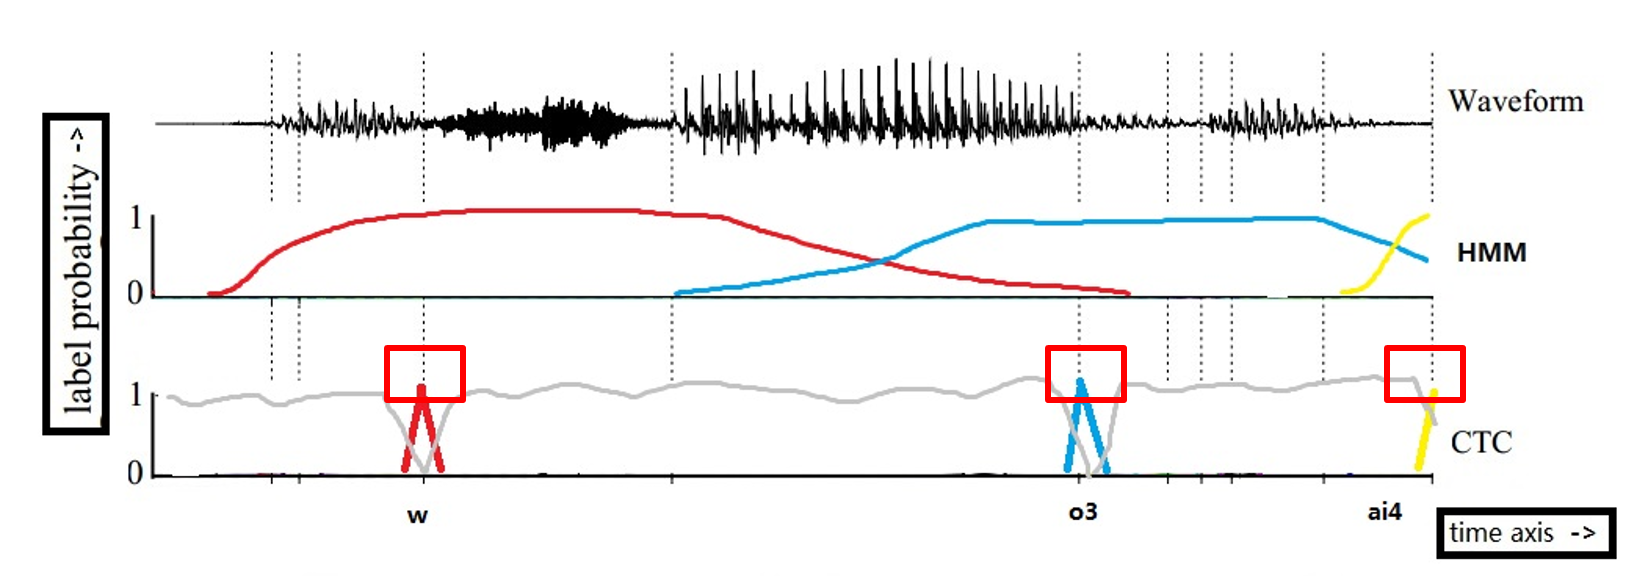
\includegraphics[width=\textwidth]{figure/peaky_distribution.png}
    \bicaption[fig:peaky-dist]{HMM,CTC的模型输出分布示例}{HMM,CTC的模型输出分布示例。纵轴表示模型输出概率,横轴表示时间。灰色分布表示CTC模型的$\tt blank$概率输出}{Fig}{The inference distributions of HMM and CTC models.}
\end{figure}


\section{基于连接时序分类模型的标签同步解码}
\label{chap:lsd-ctc}


该部分中,本章节提出将搜索过程从特征层面改为标签层面,称为标签同步解码(Label Synchronous Decoding, LSD)。本部分将对DSM中的LSD进行公式推导,具体实现方案及一些解码加速的经验方案也将进行讨论。

\subsection{标签同步解码}
\label{chap:lsd-lsd-ctc-method}
在测试阶段,在基于音素的CTC模型中,从公式 \ref{eq:asr-dec}可以推导出公式\ref{eq:ctc-dec}。 而根据CTC中输出标签之间的条件独立性假设,$P(\mathbf{l}|\mathbf{x})$可以如下获得:
\begin{equation} \label{eq:indep-output-ctc}
  \begin{split}
        P(\mathbf{l}|\mathbf{x}) 
        = \prod_{l\in\mathbf{l}} P(l|\mathbf{x}) \end{split}
       \end{equation}

因此在标签级别上, 维特比搜索如下所示:
\begin{equation} \label{eq:ctc-dec-lsd}
   \mathbf{w}^* = \mathop{\arg\!\max}\limits_\mathbf{w} \left\{
        P(\mathbf{w})
        \mathop{\max}\limits_{\mathbf{l}_\mathbf{w}} \frac{ \prod_{l\in\mathbf{l}_\mathbf{w}} P(l|\mathbf{x}) }{P(\mathbf{l}_\mathbf{w})}\right\}
     \end{equation}

在音素级的$P(l|\mathbf{x})$的计算过程中,本章节提出在帧级神经网络的输出上进行一步后处理,以便滤除$\tt blank$输出,仅保留非$\tt blank$的音素输出概率来进行公式(\ref{eq:ctc-dec-lsd})的解码搜索。本章节定义公共$\tt blank$帧的集合如下:
  \begin{equation} \label{eq:com-blk-idx}
    U=\{u:y^{u}_{\tt{blank}} > \mathcal{T}\}
%    u \triangleq \left\{
%    \begin{aligned}
%    \pi\in \{\mathcal{B}(\pi_{1\mathord{:}t})=\mathbf{l}_\mathbf{w} \} \\
%    \forall \pi_u=blank
%    \end{aligned}
%    \right.
    \end{equation}
其中$y^{u}_{\tt{blank}}$ 是神经网络在第 $u$ 帧输出$\tt blank$单元的概率。在CTC模型中的softmax层,如果$\tt blank$单元的声学得分足够大且接近常数1,则可以认为所有竞争路径共享相同跨度的$\tt blank$帧。 因此,忽略这些帧的分数并不会影响解码中的声学得分排序。
  \begin{equation} \label{eq:viterbi-blk-ctc}
  \begin{split}
      P(l|\mathbf{x})
      =\sum_{\pi\in\mathcal{B}(\mathbf{l})}
          \ \prod_{\pi}P(\pi|\mathbf{x})\\
      %TODO pi
        \simeq\sum_{\pi\in\mathcal{B}(\mathbf{l})}
         \  \prod_{\pi\in U}{y_{b_l}^u}{\prod_{\pi\not\in U}{y_{p_l}^u}}
        %\\ 
%        =
        %\sum_{\pi:\pi \in L',\mathcal{B}(\pi_{1\mathord{:}T})=l}
           %{\prod_{\pi\not\in U}{P(\pi|\mathbf{x})}}{\prod_{\pi\in U}{P(\pi|\mathbf{x})}}\\
%           \simeq 
                   %\sum_{\pi:\pi \in L',\mathcal{B}(\pi_{1\mathord{:}T})=l}
           %{\prod_{\pi\not\in U}{P(p|\mathbf{x})}}{\prod_{\pi\in U}{P(b|\mathbf{x})}}
        \end{split}
       \end{equation}


由于$\prod_{\pi\in U}{y_{b_l}^u}\simeq 1$,公式\ref{eq:viterbi-blk-ctc}可被推导为\ref{eq:viterbi-blk-ctc-sim}:
  \begin{equation} \label{eq:viterbi-blk-ctc-sim}
  \begin{split}
      P(l|\mathbf{x})
      %TODO pi
        \simeq\sum_{\pi\in\mathcal{B}(\mathbf{l})}
         \  {\prod_{\pi\not\in U}{y_{p_l}^u}}
        %\\ 
%        =
        %\sum_{\pi:\pi \in L',\mathcal{B}(\pi_{1\mathord{:}T})=l}
           %{\prod_{\pi\not\in U}{P(\pi|\mathbf{x})}}{\prod_{\pi\in U}{P(\pi|\mathbf{x})}}\\
%           \simeq 
                   %\sum_{\pi:\pi \in L',\mathcal{B}(\pi_{1\mathord{:}T})=l}
           %{\prod_{\pi\not\in U}{P(p|\mathbf{x})}}{\prod_{\pi\in U}{P(b|\mathbf{x})}}
        \end{split}
       \end{equation}

\subsection{标签同步解码算法实现}
\label{chap:lsd-lsd-ctc-alg}

DSM的标签同步解码算法如算法~\ref{code:lsd-dsm-alg}所示。S和E是预编译的WFST网络的起始和结束节点。Q指有效令牌,B ̂指解码路径,T是总帧数。$NNPropagate(t)$ 是每帧的声学模型推理过程。$isBlankFrame(F)$ 用于检测每帧是否为$\tt blank$。 $ViterbiBeamSearch(F, Q)$是FSD中的标准维特比搜索算法,在算法\ref{code:tokpass}中的第7行进行定义,但在LSD中仅在标签级别执行。  $finalTransition(E,S,Q)$用于搜索WFST的终止节点\cite{hori2007efficient}。


\begin{algorithm}[ht]
\caption{DSM的标签同步维特比束搜索算法 \textcolor[rgb]{0,0.5,0}{(Inputs: 起始节点,结束节点,令牌队列,时间帧)}}
\label{code:lsd-dsm-alg}
\begin{algorithmic}[1]
\Procedure{ LSD for DSM } {S, E, Q, T}
\State $Q \leftarrow S$ \Comment \textcolor[rgb]{0,0.5,0}{起始节点初始化}
\For {each $t\in [1,T]$}    \Comment \textcolor[rgb]{0,0.5,0}{逐帧神经网络前向传播}
\State $F \leftarrow NNPropagate(t)$
\If {!isBlankFrame($F$)}   \Comment \textcolor[rgb]{0,0.5,0}{逐音素解码}
\State  $Q\leftarrow ViterbiBeamSearch(F, Q)$
\EndIf
\EndFor
\State $\hat B\leftarrow finalTransition(E,S,Q)$ \Comment \textcolor[rgb]{0,0.5,0}{到达结束节点}
\State backtrace($\hat B$)
\EndProcedure
\end{algorithmic}
\end{algorithm}


\section{基于无词图鉴别性训练模型的标签同步解码}
\label{chap:lsd-lfmmi}

\subsection{标签同步解码}
\label{chap:lsd-lsd-hmm}

在基于LF-MMI的生成式序列模型(Generative Sequence Model, GSM)中,相邻HMM之间的输出标签也是条件独立的:
\begin{equation} \label{eq:viterbi-blk-hmm}
  \begin{split}
        P(\mathbf{x}|\mathbf{l}) 
        = \prod_{l} P(\mathbf{x}|l) \end{split}
       \end{equation}

类似地,在标签级别上进行的维特比搜索如下所示。
\begin{equation} \label{eq:gsm-dec-lsd}
   \mathbf{w}^* = \mathop{\arg\!\max}\limits_\mathbf{w} \left\{
        P(\mathbf{w})
        \mathop{\max}\limits_{\mathbf{l}_\mathbf{w}}  \prod_{l\in\mathbf{l}_\mathbf{w}} P(\mathbf{x}|l)\right\}
     \end{equation}

在标签中, $P(\mathbf{x}|l)$ 的计算如下所示:
\begin{equation} \label{eq:viterbi-blk-gsm}
  \begin{split}
        P(\mathbf{x}|l)
        = \sum_{\pi:\pi \in L',\mathcal{A}(\pi_{1\mathord{:}T})=l}
          \ \prod_{t=1}^{T} P(\mathbf{x}|\pi_t)P(\pi_t|\pi_{t-1})\\
= \sum_{\pi:\pi \in L',\mathcal{A}(\pi_{1\mathord{:}T})=l}
          \ \prod_{t=1}^{T} P(\pi_t|\mathbf{x})\frac{P(\pi_t|\pi_{t-1})}{P(\pi_t)}
        \end{split}
       \end{equation}  
其中 $\pi_t $是帧t的推理搜索模型单元。
我们在第\ref{Sec:lfmmi-train}章节介绍了几种本文所扩展的HMM拓扑结构,如图~\ref{fig:hmm-topo}(c-e)。虽然在我们的实验中,这些模型的输出分布比CTC中更平滑,但DSM中提出的公式~(\ref{eq:com-blk-idx}) 和 (\ref{eq:viterbi-blk-ctc})可以被扩展到GSM。


这里提出对神经网络的输出$P(\pi_t|\mathbf{x})$ 进行后处理。由于这些模型中的模拟$\tt blank$状态,公式\ref{eq:gsm-dec-lsd}中的维特比束搜索不必包括标签输出候选序列的所有帧。因此,给出某一帧的模型推理搜索分布时,是否从维特比搜索中排除某帧的判决如下:
  \begin{equation} 
       \label{eq:com-blk-idx-gsm}
       \begin{split}
U=\{u:\sum_{l\in L}(y^{u}_{b_l}-y^{u}_{p_l})> \mathcal{T}\}
\end{split}
\end{equation}
其中 $y^{u}_{p_l}$ 是帧u处标签输出状态l的神经网络输出,$y^{u}_{b_l}$ 是对应的$\tt blank$状态的输出。在第u帧是否有标签输出,是由所有$\tt blank$状态与标签输出状态的概率差异的总和决定的。T是在开发集中得到的阈值。因此, $P(\mathbf{x}|l)$  的计算可以根据 $\pi\in U$与否分为如下两部分:
\begin{equation} \label{eq:viterbi-blk-hmm2}
  \begin{split}
P(\mathbf{x}|l)
\simeq\sum_{\pi:\pi \in L',\mathcal{A}(\pi_{1\mathord{:}T})=l}
         \{\   \\ %P(b_l|p_l)P(p_l|b_l)
         \prod_{\pi\not\in U}\frac{y_{b_l}^u P(b_l|\mathbf{x})}{P(b_l)} \prod_{\pi\in U}\frac{y_{p_l}^u P(p_l|\mathbf{x})}{P(p_l)}
         \}
         \end{split}
       \end{equation}   
其中第一部分是标签输出状态。在该情况下,每个标签输出均在WFST中进行维特比搜索。而另外一组的$\tt blank$部分,则假设没有标签输出。不同于CTC,不同标签输出维护自己的$\tt blank$状态版本。即使是$\tt blank$帧,也可能包含不同的输出标签信息。因此, $\prod_{\pi\not\in U}\frac{y_{b_l}^u P(b_l|\mathbf{x})}{P(b_l)}$的分数不能被丢弃。下文提出一种高效的算法对这一项进行计算。

这里所提出的后处理可以被视为输出标签概率$P(\pi|\mathbf{x})$的近似,从而使得维特比束搜索得以在标签级别上进行。


\subsection{标签同步解码算法实现}
\label{chap:lsd-lsd-hmm-alg}

用于GSM的标签同步解码算法如算法\ref{code:lsd-gsm-alg}所示。与算法\ref{code:lsd-dsm-alg}相比,在每个$\tt blank$帧中,输出序列可以包含不同的$\tt blank$单元。因此对相邻的$\tt blank$帧计算$\prod_{\pi\not\in U}\frac{y_{b_l}^u P(b_l|\mathbf{x})}{P(b_l)}$ 。在非$\tt blank$帧中,首先将各个$\tt blank$单元各自累积得到的概率得分分别添加到当前帧的所有候选序列分数中,之后再进行维特比搜索算法。这些不同之处在算法中使用红色字体来表示。


\begin{algorithm}[ht]
\caption{GSM的标签同步维特比束搜索算法\textcolor[rgb]{0,0.5,0}{(Inputs: 起始节点,结束节点,令牌队列,时间帧)}}
\label{code:lsd-gsm-alg}
\begin{algorithmic}[1]
\Procedure{ LSD for DSM } {S, E, Q, T}
\State $Q \leftarrow S$ \Comment \textcolor[rgb]{0,0.5,0}{起始节点初始化}
\For {each $t\in [1,T]$}    \Comment \textcolor[rgb]{0,0.5,0}{逐帧神经网络前向传播}
\State $F \leftarrow NNPropagate(t)$
\If {!isBlankFrame($F$)}    \Comment \textcolor[rgb]{0,0.5,0}{逐音素解码}
\State  {\color{red}{$F \leftarrow addAccumulatedBlankScore(V,F)$ }}
\State  {\color{red}{$reset(V)$ }}
\State  $Q\leftarrow ViterbiBeamSearch(F, Q)$
\Else         \Comment \textcolor[rgb]{0,0.5,0}{accumulate $\tt blank$ scores}
\State  {\color{red}{$V \leftarrow accumulateBlankScore(V,F)$ }}
\EndIf
\EndFor
\State $\hat B\leftarrow finalTransition(E,S,Q)$ \Comment \textcolor[rgb]{0,0.5,0}{到达结束节点}
\State backtrace($\hat B$)
\EndProcedure
\end{algorithmic}
\end{algorithm}


除此之外,在HMM拓扑结构方面,本章节将第\ref{Sec:lfmmi-train}章节提出的图\ref{fig:hmm-topo}(d-e)所示的几种改进结构都应用在了GSM中。

本章节在维特比搜索中除了使用传统的束剪枝算法\cite{forney1973viterbi}和直方图剪枝算法\cite{steinbiss1994improvements}(自适应束剪枝\cite{van1996adaptive})之外,提出了另外两种剪枝方法。 在LSD中,$\tt blank$帧占总帧数的百分比与加速比成正比,而$\tt blank$帧通过公式进行判定。作为束剪枝算法的变体,这里提出了基于$\tt blank$帧阈值T的剪枝算法,称为$\tt blank$剪枝。当阈值T固定时,推理搜索分布的尖峰属性决定了加速比,而尖峰属性显示了神经网络输出分布的置信度。在神经网络的模型训练阶段,本章节又提出了基于假设剪枝的熵剪枝算法。 在文献\cite{pereyra2017regularizing}中,作者通过惩罚确定的输出分布来防止过拟合和提高神经网络的泛化能力。受这项工作的启发, 我们在LSD框架中对输出分布的熵进行了控制,作为候选序列的剪枝方法。具体来说,在模型训练中将输出分布的熵添加到负对数似然$\mathcal{L}(\theta)$中,公式如下所示:
  
\begin{equation}
\label{equ:ent-pen-model}
\begin{split}
\mathcal{L}(\theta)= - (\ p_\theta (\pi|\mathbf{x}) - \beta H(p_\theta (\pi|\mathbf{x})\ )
\end{split}
\end{equation}
其中$H(\cdot)$是输出分布 $p_\theta (\pi|\mathbf{x})$的熵,$\beta$是正比例因子。与文献\cite{pereyra2017regularizing}不同的是,基于熵剪枝算法的训练目的是最小化模型的原有训练准则以及输出分布的熵。而通常情况下,基于熵剪枝算法是基于一个已经训练好的模型对参数进行微调。在使用新的准则训练之后,LSD框架可在少量性能损失的情况下得以加速。在接下来的实验部分,本章节将详细比较这四种剪枝方法。


\section{标签同步解码的进一步分析}
\label{chap:lsd-lsd-more}

\subsection{逐帧同步解码与标签同步解码的对比}
\label{chap:lsd-lsd-cmp}

本章节提出将特征层面的搜索过程改变为标签层面,即搜索空间是由不同历史的标签组成的,使得解码速率等于标签速率,从而小于特征速率。具体来说,所提出的LSD的解码复杂度如下:
  \begin{equation}
\label{equ:complex-lsd}
\begin{split}
\mathbb{C}_{LSD} = O (T-|U|) \ \mathbb{C}_{frame}
\end{split}
\end{equation}
其中空白帧的数量 $|U|$,总是接近于T。对比公式(\ref{equ:complex-fsd})和公式(\ref{equ:complex-lsd}),FSD得到了很大的加速。这里将FSD和LSD之间的主要区别总结如下:
\begin{itemize}
\item 不同的信息率。 在FSD中,声学和语言信息均在每帧进行处理,使得二者的处理速率均和声学特征的帧率相同。而在LSD中,声学信息是以声学特征的帧率进行处理的,而语言信息则按声学模型推理的标签速率进行处理。声学和语言信息处理的不同速率去除了大量的搜索冗余。
\item 可调整的搜索间隔。 在FSD框架下,WFST网络是以等间隔遍历的。即使带有跳帧的深度神经网络在解码\cite{vanhoucke2013multiframe}时是以更长的间隔遍历语言搜索空间,但其间隔仍然是相等的。 而在LSD中,搜索间隔可通过灵活的自我调整(在不造成性能下降的前提下)来去除$\tt blank$帧带来的语言搜索空间搜索冗余,这给解码带来了很大的效率提升。另一方面,由于LSD方法与跳帧方法工作在不同层面,因此它们可以互相结合取得进一步的加速,这些我们将在实验章节中具体验证。
\end{itemize}

\subsection{标签同步的词图处理}
\label{chap:lsd-lsd-lattice}

前文中我们导出了标签同步算法,使得搜索解码复杂度得到了显著下降。
除此之外,这一算法同时还能产生高质量的音素词图,称为标签同步音素词图(LSD音素词图)。

LSD音素词图可以很好地保存音素级的声学候选信息,同时得益于前文的加速算法,又非常紧致。
%
以CTC 模型为例,其模型尝试对多对一函数$\mathcal{B}$进行建模,使得最终结果能得到非常突出的音素推理搜索结果。
LSD音素词图是从丢弃了一定数量的 $\tt blank$ 帧的推理搜索分布中生成得到的,之后可以将剩余帧的一定阈值以内的音素后验概率收集起来组成时间上不连续的词语串。这样的方式避免了一些搜索错误和混淆的音素边界问题,使得最终得到的词图更紧致。
%
图\ref{fig:ctc-lat-exp}是一个用WFST格式表示的LSD音素词图的例子。
WFST可以如图这样构建成“串(sausage)”状。这里每两个音素输出帧之间,使用以音素标签为输出,以负声学分数为权重的WFST边,来互相连接起来。WFST边的输入使用epsilon,这样就可以对LSD音素词图进行进一步的 WFST优化处理。

\begin{figure}[!htp]
  \centering
    \captionstyle{\centering}
    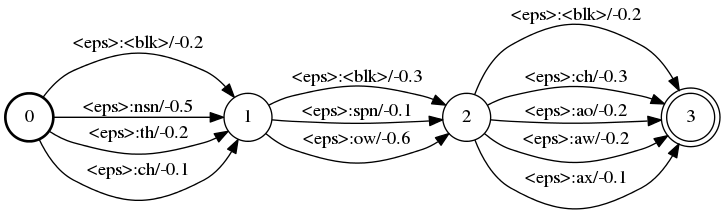
\includegraphics[width=\textwidth]{figure/ctc_lat.png}
    \bicaption[fig:ctc-lat-exp]{LSD CTC Lattice的例子}{LSD CTC Lattice的例子}{Fig}{The example of LSD CTC Lattice.}
\end{figure}

我们可以将LSD音素词图视为一种特殊形式的词图,因此与逐帧的音素后验概率相比,它非常紧致,节省了大量存储空间。
同时LSD音素词图自然地由逐帧的音素后验概率得到,类似于一种基于$\tt blank$建模而产生的特殊高效的特征提取,因此与普通词图相比,其包含更多的可能候选路径,信息损失非常小。

我们将在第\ref{sec:exp-lsd-lat-quality}章节通过实验验证其质量。基于LSD音素词图,下一章节将进一步探讨标签同步解码算法的一些扩展应用。

\section{实验结果}
\label{chap:lsd-exp}

本章节实验使用300小时的英语Switchboard数据集作为训练数据\cite{godfrey1992switchboard},使用NIST 2000 CTS作为测试集,对NIST 2000 CTS测试集所包含的switchboard(称为swb)和call-home(称为callhm)两个子集分别进行了评估。在所有实验中使用的是经过工程优化的标准WFST解码器;实验过程中没有生成词图,也没有使用语言模型重打分~\cite{povey2012generating}技术。解码过程中使用在Switchboard和Fisher转录文本上训练的插值的4阶语言模型;在CTC算法验证中,默认使用了经过剪枝的3阶语言模型;在LF-MMI算法验证中,默认使用4阶语言模型,使得结果与文献~\cite{povey2016purely}具有可比性。解码使用的机器配置为Intel(R)Xeon(R)CPU E5-2690 v2 @ 3.00GHz。

本章节的CTC实验中,使用具有1.2 M参数的小型CTC模型,使得其适用于嵌入式设备,与文献 \cite{mcgraw2016personalized}可比;使用40维的对数滤波器组特征,特征提取窗宽为25 ms,帧移为10 ms;使用46个单音素作为声学建模单元;声学模型使用3层带有投影层的长短时记忆网络,每层包括400个节点并通过投影层压缩为128个节点~\cite{sak2014long};使用EESEN \cite{miao2016ctc}作为训练工具,训练过程与文献~\cite{miao2015eesen}相似。

本章节的LF-MMI实验是在一系列由KALDI流程\cite{povey2011kaldi}训练的基于HMM的大型模型上进行的,这些模型均适用于服务器应用。声学模型建模单元是上下文相关音素。为了提升解码性能~\cite{pundak2016lower,povey2016purely},相对于输入层特征10 ms每帧的帧率,将输出层的输出帧率下降到30 ms每帧。声学模型分别使用每层625个节点的7层时延神经网络(TDNN);以及3层带有投影层的双向长短时记忆网络(BLSTM),其中每层的前向后向层均具有1024个节点,并通过投影层压缩为256个节点。

本章节实验过程中,使用词错误率(word error rate, WER)来评估不同解码框架下的模型性能, 使用搜索过程中的实时率(real time factor (RTF) of the search process)和每帧中的活动令牌的平均数量(active tokens, \#AT)来评价搜索速度,它们都在第\ref{chap:intro-lvcsr-criterion}章节进行了介绍。在降低帧率的声学模型中,\#AT使用降帧率之前的帧数进行计算;RTF指解码时间与音频时间的百分比。值得注意的是,这里用于计算RTF的解码时间不包括神经网络传播的时间\cite{you2009parallel,hauswald2015sirius}。本章节所提出的框架主要加速搜索过程而非神经网络传播,因此不针对不同声学模型的计算速度进行比较,同时这里采用的RTF只包括搜索解码的时间。由于在维特比搜索的搜索迭代过程-即令牌传递算法~\cite{hori2013speech}中,搜索迭代速度与有效令牌的数量相关,因此搜索速度评价指标AT与RTF总是正相关。为了更加清晰地对比结果,我们还提供了上述指标的相对变化率($\Delta$)作为参考。

\subsection{CTC实验}
\label{exp:dsm}

(1)加速:表1给出了CTC模型下,LSD系统相对FSD系统的加速对比。基于FSD的CTC模型是基线系统。在我们的这项工作中\cite{7736093}曾进一步对比了CTC模型的性能和基于HMM的系统的性能。


\begin{table}[thbp!]
  \caption{\label{tab:exp-lsd-fsd-dsm} {\it LSD versus FSD in CTC}}
  \centerline{
  \begin{tabular}{ m{0.1\columnwidth} ||m {0.08\columnwidth} m {0.08\columnwidth} |m {0.08\columnwidth} m {0.08\columnwidth} m {0.08\columnwidth} m {0.08\columnwidth}}
\toprule
\multirow{3}{0.1\columnwidth}{测试子集  }  &
\multicolumn{2}{c|}{解码性能   }& 
\multicolumn{4}{c}{搜索加速} 
\\
&\multicolumn{2}{c|}{FSD$\mapsto$LSD}&\multicolumn{2}{c}{FSD$\mapsto$LSD}&\multicolumn{2}{c}{FSD$\mapsto$LSD}\\
&WER&$\Delta$(\%)&RTF&$\Delta$(\%)&\#AT&$\Delta$(\%)\\
\midrule
% https://spetechcular.com/trac/aid201501/wiki/20161011lfmmi-research#modifyHMM
\multirow{1}{0.15\columnwidth}{swb} &  18.7 &+0.5&0.075&-71&2221&-77  \\
%\hline\hline
\multirow{1}{0.15\columnwidth}{callhm} &  33.3 &+0.0&0.073&-70&2211&-77 \\
\bottomrule
\end{tabular}
  }
\end{table}

swb测试子集中,在词错误率相对损失不到0.5\%的情况下,与FSD框架相比,LSD框架实现了相对70\%以上的RTF下降(也就是3.4倍的解码加速)。解码加速主要来自于解码过程中减少了搜索迭代次数,解码过程中的活动令牌的数量也体现了这一结果。同时在callhm子集的实验中也能观察到一致的加速效果。

(2)速度鲁棒性:上面的实验解码过程中都使用一个中等大小的语言模型(3阶,3.1 M语言模型),为了测试LSD框架相对于FSD加速效果的鲁棒性(也即对复杂的语言搜索空间下的可扩展性),如图2所示,这里将解码语言模型从2阶变大到4阶,大小从0.2 M变大到4.7 M,使用每帧中的平均活动令牌数(\#AT)来评价解码速度。从图 ~\ref{fig:ctc-dnn-lm-scaleup} 中可以看出,随着语言模型的增大,LSD的\#AT值几乎没有变化,而与此同时,FSD的 \#AT值则明显加速增长。此外,FSD的\#AT值总是远远超过LSD的\#AT值。也就是说,LSD实现的加速对LM搜索空间的增加是鲁棒的,LF-MMI的实验也得出了类似的结论,因此LSD适合应用于更复杂的语言模型。
 

\begin{figure}[htb]
  \centering
    \captionstyle{\centering}
    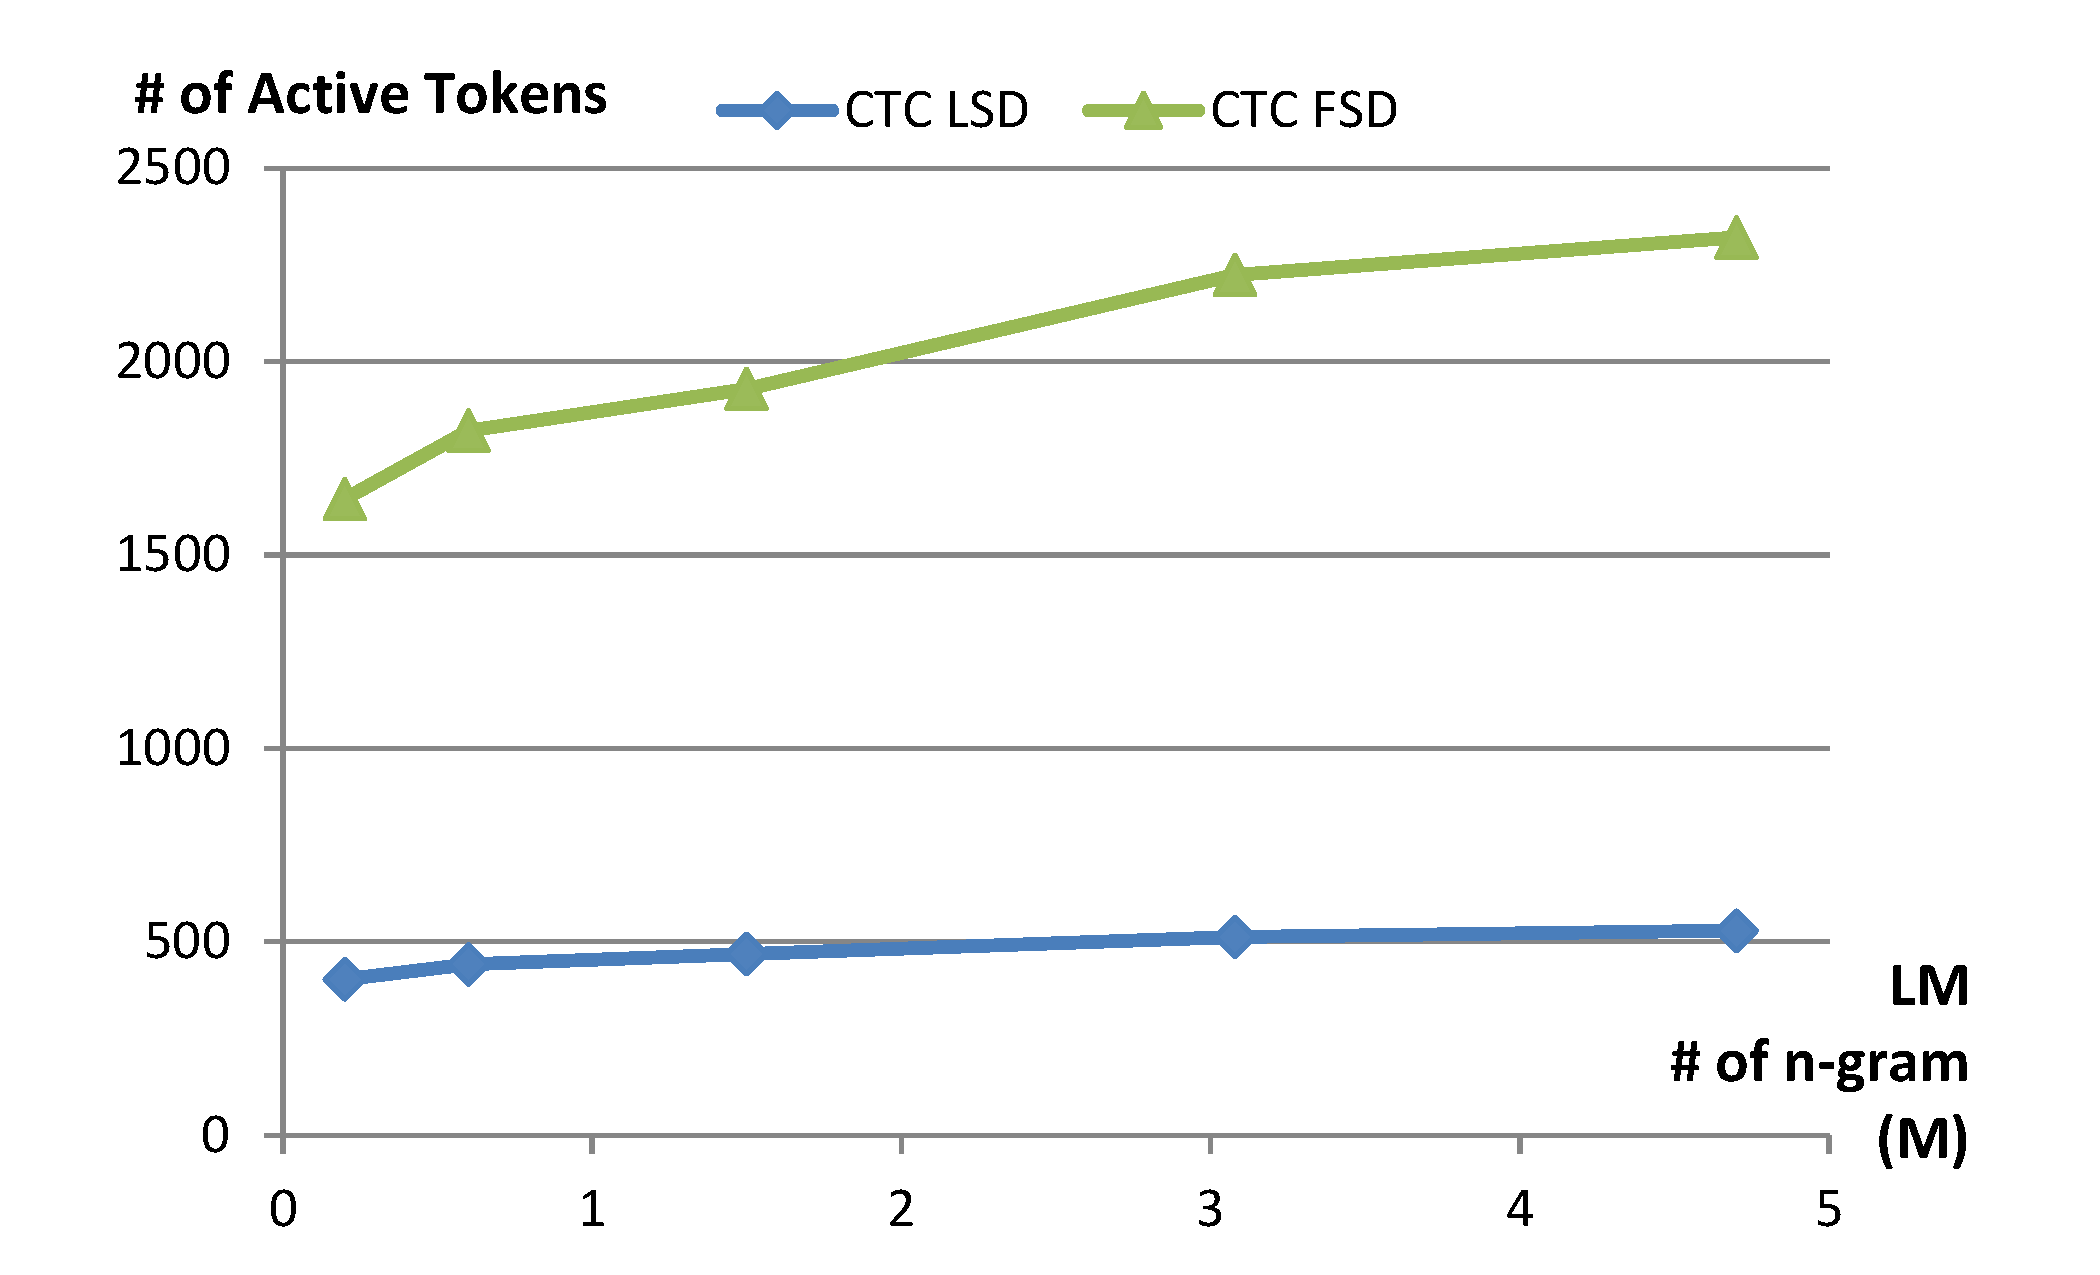
\includegraphics[width=0.8\textwidth]{figure/speed-robust.pdf}
    \bicaption[fig:ctc-dnn-lm-scaleup]{LSD和FSD框架中平均活跃令牌数随LM变大的变化趋势}{LSD和FSD框架中平均活跃令牌数随LM变大的变化趋势。为清晰起见,这里仅绘制swb子集,calhm子集具有类似变化趋势。}{Fig}{The trend of average active token numbers and the sizes of LMs in LSD and FSD based frameworks.}
\end{figure}


(3)结合跳帧方法:该部分对比了跳帧方法下的LSD与FSD框架,实现结果表明可以将跳帧方法与FSD框架进行结合使用。值得注意的是,在后面的实验中,LSD也可以应用于跳帧或降低帧率的LF-MMI声学模型中。

跳帧的实现方法类似于文献\cite{miao2016simplifying},这里使用LSTM-CTC的2倍跳帧(FS),并且在神经网络后验概率输出层上没有根据原始特征帧率补全后验概率,因此FS也可以加速解码过程。该方法在没有性能损失的情况下,应用于CTC模型的FS可以获得近2倍的解码性能加速。这与文献~\cite{pundak2016lower}中的观察结果一致,并且在LSTM-HMM\cite{miao2016simplifying}和DNN-HMM\cite{vanhoucke2013multiframe}也有类似的结果。LSD可以进一步与FS组合,并且获得更高的效率,即在搜索过程中进一步减少57\%(累计为78\%)的时间。


\begin{table}[thbp!]
  \caption{\label{tab:exp-cmp-vfr-lsd-dsm} {\it LSD与跳帧方法的对比}}
  \centerline{
  \begin{tabular}{ m{0.1\columnwidth} ||m {0.08\columnwidth} m {0.08\columnwidth} |m {0.08\columnwidth}  m {0.08\columnwidth} m {0.20\columnwidth} }
\toprule
\multirow{3}{0.1\columnwidth}{测试子集}  &
\multicolumn{2}{c|}{解码性能  }& 
\multicolumn{3}{c}{搜索加速} 
\\
&\multicolumn{2}{c|}{FSD$\mapsto$FS+LSD}&\multicolumn{3}{c}{FSD$\mapsto$FS$\mapsto$FS+LSD}\\
&WER&$\Delta$(\%)&RTF&$\Delta_{FS}$&$\Delta_{+LSD} $ ($\sum$)\\
\midrule
% https://spetechcular.com/trac/aid201501/wiki/20161011lfmmi-research#modifyHMM
\multirow{1}{0.15\columnwidth}{swb} &  18.7 &-1.6&0.075&-48&-57 (-78)  \\
\multirow{1}{0.15\columnwidth}{callhm} &  33.3 &-0.6&0.073&-47&-57 (-77) \\
\bottomrule
\end{tabular}
  }
\end{table}

(4)候选序列剪枝:图\ref{fig:prune-wer-at-dsm}比较了本章节提出的LSD框架与传统的剪枝技术,即束剪枝(表示为beam)和直方图剪枝(表示为histogram)。 在LSD中,通过调整公式\ref{eq:com-blk-idx}和\ref{eq:com-blk-idx-gsm}中定义的T来调整加速比和性能,这也可以被视为另一种候选序列剪枝方法(表示为$\tt blank$)。 上文中提出的基于熵剪枝算法表示为entropy。
 

\begin{figure}[htb]
  \centering
    \captionstyle{\centering}
    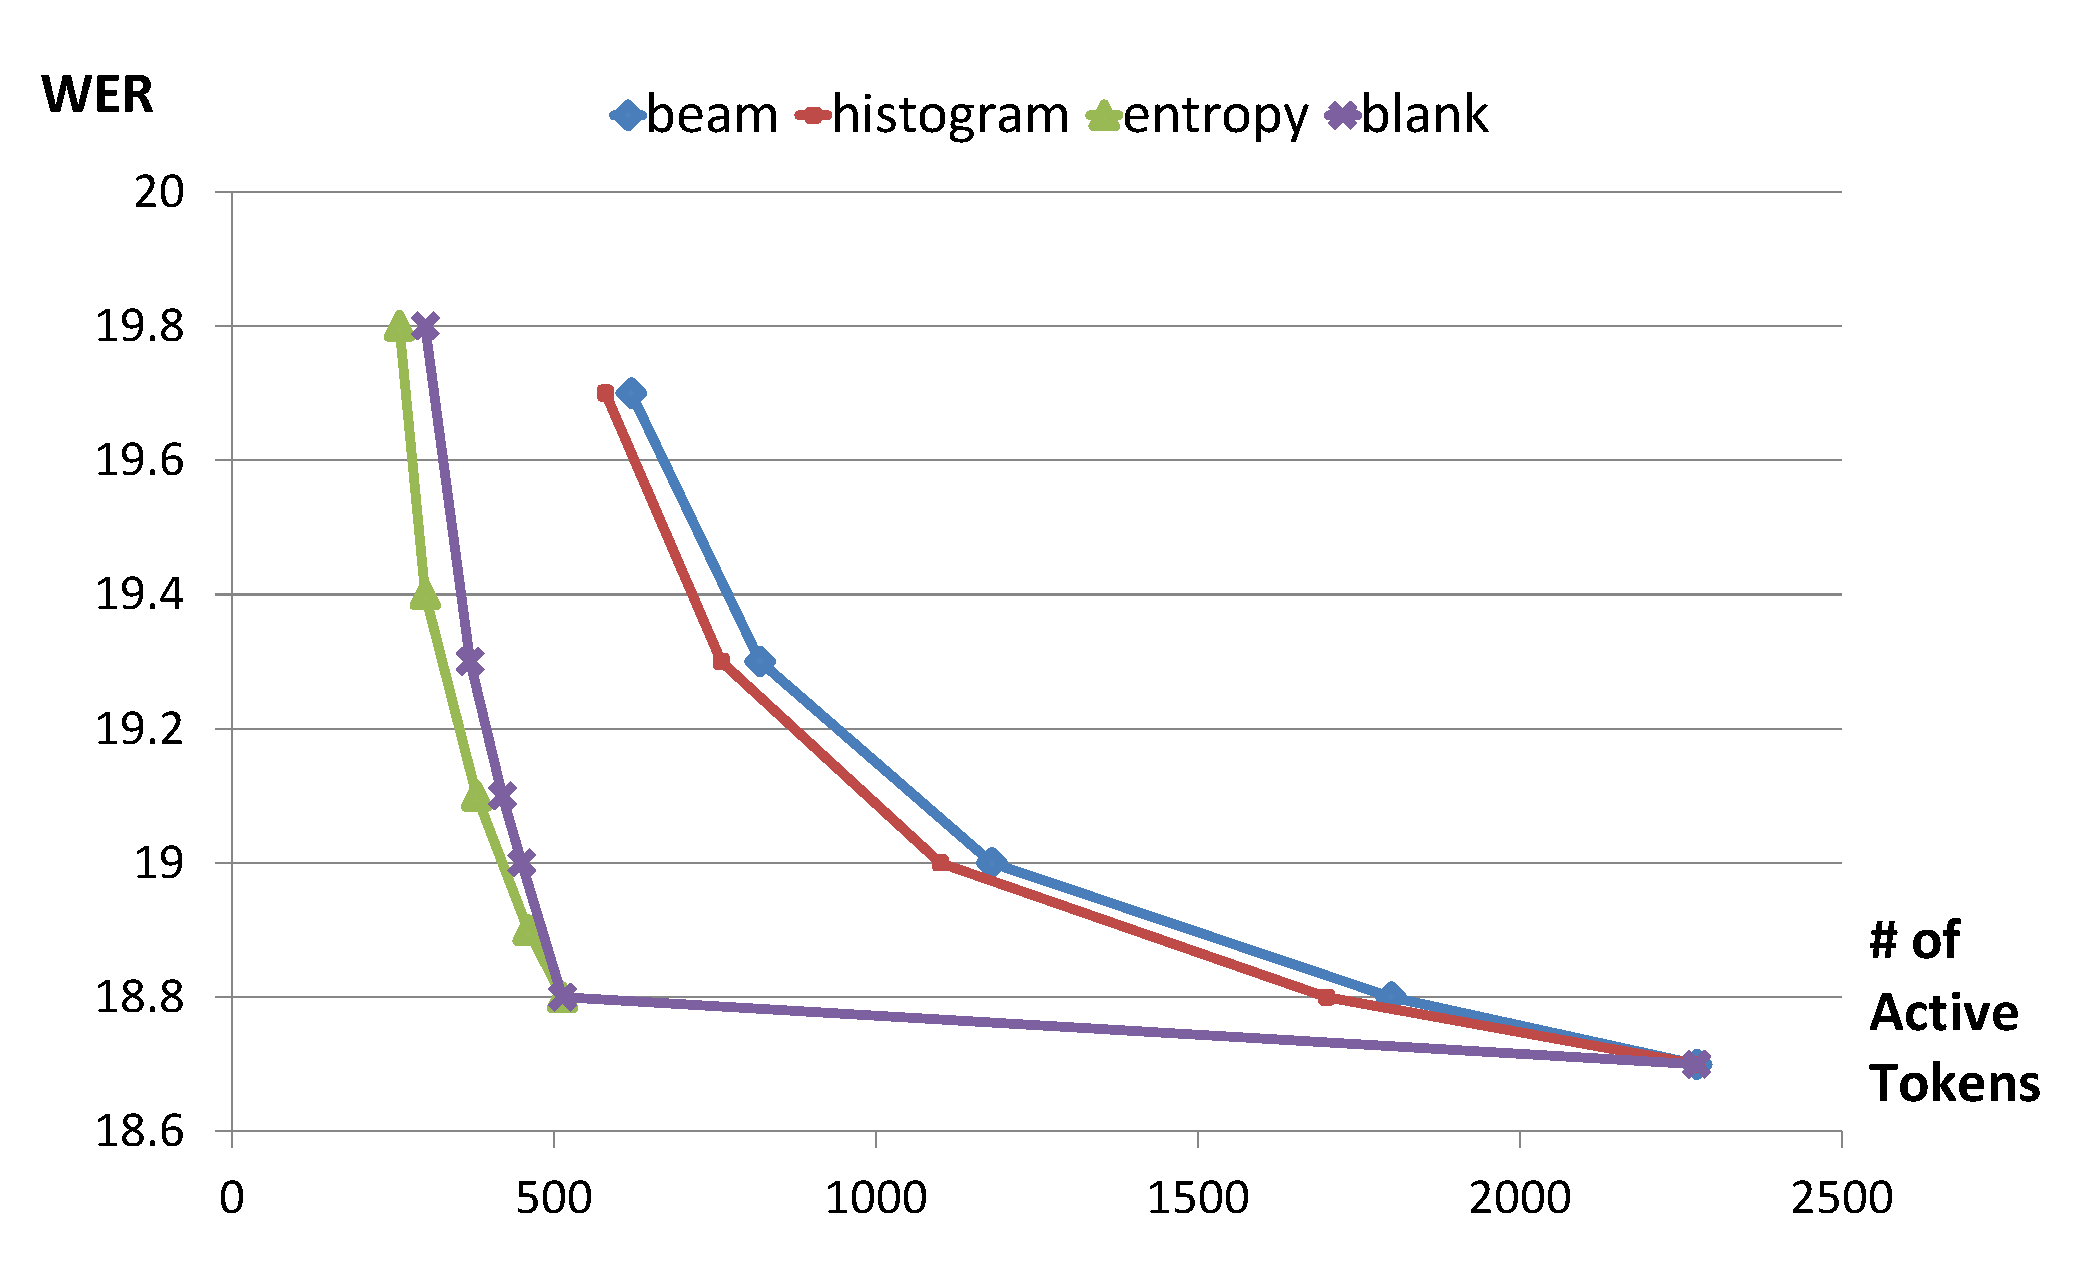
\includegraphics[width=0.8\textwidth]{figure/prune-wer-at-dsm.pdf}
    \bicaption[fig:prune-wer-at-dsm]{swb子集,CTC中,使用不同剪枝技术时WER随平均活跃令牌数的变化趋势}{swb子集,CTC中,使用不同剪枝技术时WER随平均活跃令牌数的变化趋势。calhm子集结果类似}{Fig}{The trend of WER v.s. the number of active tokens using different pruning methods in CTC and swb-subset.}
\end{figure}


从图中可以看出,基于LSD的方法,entropy和$\tt blank$,与基于FSD的方法beam和histogram相比保持显著优势。其原因在于,基于FSD的候选序列剪枝对所有候选序列进行统一处理,而相反,LSD框架可以看作是将候选序列划分为特征级别和标签级别。因此,如公式\ref{eq:ctc-dec-lsd}及公式\ref{eq:com-blk-idx}所示,LSD框架中,可以在特征层和标签层进行剪枝。也即,基于LSD的候选序列剪枝方法受益于将搜索过程从特征层转移到标签层。

另外结果显示,为了加速解码,两种框架中的方法都会降低解码性能,而且基于LSD的方法解码性能下降更严重。如前所述,基于FSD和LSD的方法之间的关键区别在于后者的阈值T仅与特征层上的候选序列剪枝有关。特征层候选序列剪枝的加速比几乎是固定的,在不损害性能的情况下,70-80\%的候选序列可以被剪枝掉。图\ref{fig:prune-wer-at-dsm}中$\tt blank$曲线具有明显的拐点(\#AT = 513,WER = 18.8),也源于同样的原因。在图的最右侧,未进行特征层剪枝时,$\tt blank$曲线最终达到了与基于FSD的方法的同一点。由于上面讨论的明显拐点及固定加速比,可以很容易得到等式\ref{eq:ctc-dec-lsd}中的阈值T。此外,特征层的entropy和$\tt blank$剪枝可以进一步与标签层的beam和histogram方法相结合,以得到最佳的解码加速效果。为了使对比更加清晰,图中没有给出融合系统的曲线。

最后,entropy的效率略高于$\tt blank$(相对约10\%)。我们认为原因在于神经网络中剪枝能更好地利用神经网络输出分布中的信息,并且产生更好的精度和效率。而$\tt blank$剪枝则仅利用了输出分布中的最佳分数而未使用整个分布的信息。

\subsection{LF-MMI实验}
\label{exp:gsm}
(1)在各种模型和准则中的应用:LSD应用于生成式序列模型(GSM)时,本章节使用了多种不同的神经网络模型结构和模型训练准则的LF-MMI模型进行对比;默认使用上下文相关的音素作为模型建模单元。表\ref{tab:exp-lsd-fsd-gsm}给出了在NIST 2000 CTS测试集合上的结果。总体而言,LSD框架也可以取得比较显著的解码加速,但是与表\ref{tab:exp-lsd-fsd-dsm}中的结果相比,解码加速性能变差。这是因为FSD基线的帧率已经降低到原来的1/3\cite{pundak2016lower}(类似前文中帧率改变技术可以与提出的LSD框架结合)。而且与表\ref{tab:exp-cmp-vfr-lsd-dsm}相比,加速比也略小,原因是这些模型的推理搜索分布概率不像CTC那样尖锐。如何在LF-MMI中获取更尖锐的推理搜索分布概率将在后续章节中进行讨论。

具体地,如表~\ref{tab:exp-lsd-fsd-gsm}所示,第一行列出了文献\cite{pundak2016lower}中提出的低帧率模型(LFR)的结果;第二行是使用LF-MMI准则\cite{povey2016purely}训练出来的结果,显示出比LFR更快的搜索速度;此外,还可以看到从FSD到LSD,基于 LF-MMI准则训练的模型可以取得更快的加速。与文献\cite{paulik2015improvements}中观察到的类似,这都源于序列区分性训练准则得到的模型相对于交叉熵准则训练的模型有更尖锐的输出概率分布。第三行表示为+ sMBR,是在LF-MMI模型的基础上,使用基于LM的sMBR准则微调模型参数得到的结果;第四、五行列出了基于增强的MMI\cite{povey2008boosted}及sMBR准则变体的无需词图的区分性训练准则取得的结果,分别表示为LF-bMMI和LF-sMBR。可以观察到,本章节提出的LSD框架在以上模型和准则中可以取得一致的解码加速。另外我们还使用了BLSTM模型,也都取得了相似结果。


     \begin{table}[thbp!]
        \caption{\label{tab:exp-lsd-fsd-gsm} {\it  LSD与FSD在不同的LF-MMI模型上的性能和速度比较}}
        \centerline{
\begin{tabular}{ m{0.1\columnwidth} |m {0.15\columnwidth} ||m {0.06\columnwidth} m {0.06\columnwidth} |m {0.06\columnwidth} m {0.06\columnwidth} m {0.06\columnwidth} m {0.06\columnwidth}}
      \toprule
      \multirow{3}{0.1\columnwidth}{模型}  &
      \multirow{3}{0.15\columnwidth}{准则} & 
      \multicolumn{2}{c|}{性能 }& 
      \multicolumn{4}{c}{速度} 
      \\
      &&\multicolumn{2}{c|}{FSD$\mapsto$LSD}&\multicolumn{2}{c}{FSD$\mapsto$LSD}&\multicolumn{2}{c}{FSD$\mapsto$LSD}\\
      &&WER&$\Delta$(\%)&RTF&$\Delta$(\%)&\#AT&$\Delta$(\%)\\
      \midrule
      \multirow{6}{0.1\columnwidth}{TDNN} & CE  & 17.8&+1.0&0.16&-38&3705&-41 \\
      & LF-MMI &15.6 &+1.0&0.13&-43 &  3386&-45\\
      %local/chain/compare_wer_general.sh tdnn_7h_sp_smbr
      & \ \ +sMBR &15.4 &+1.0&0.12&-41 & 3295 & -43 \\
      %\cline{2-5} local/chain/compare_wer_general.sh tdnn_7h_b0.1_s1_1_sp
      & LF-bMMI &15.0 &+1.0&0.11&-42 & 3198 & -44 \\
      %\cline{2-5}
      & LF-sMBR &15.3 &+1.0&0.12&-41 & 3288 & -44 \\
      \midrule
      %local/chain/compare_wer_general.sh blstm_6h_sp
      \multirow{2}{0.1\columnwidth}{BLSTM}& LF-MMI &15.2 &+1.0&0.12&-44&3290 &-47 \\
      %local/chain/compare_wer_general.sh blstm_6h_b0.2_s2_3_sp
      & LF-bMMI &14.3 &+1.0&0.11&-43& 3205&-45 \\
      \bottomrule
      %\hline\hline
      \end{tabular}
        }
      \end{table}



(2)候选序列剪枝:如图\ref{fig:prune-wer-at-gsm}所示,我们在生成式序列模型下进行了一系列候选序列剪枝相关的实验,其变化趋势类似于DSM中的结果,读者可以参考那里的讨论。与图\ref{fig:prune-wer-at-dsm}中一个区别在于,beam,histogram,blank,entropy在图\ref{fig:prune-wer-at-gsm}中的最左边位于相同点,这表明在降低帧率的情况下,后验概率层面的候选序列剪枝(blank和entropy)的最大剪枝比例较小。 然而,在解码性能的WER达到最佳时,后验概率层面的候选序列剪枝相对普通剪枝方法,仍然有接近两倍的解码加速。



\begin{figure}[!htp]
  \centering
    \captionstyle{\centering}
    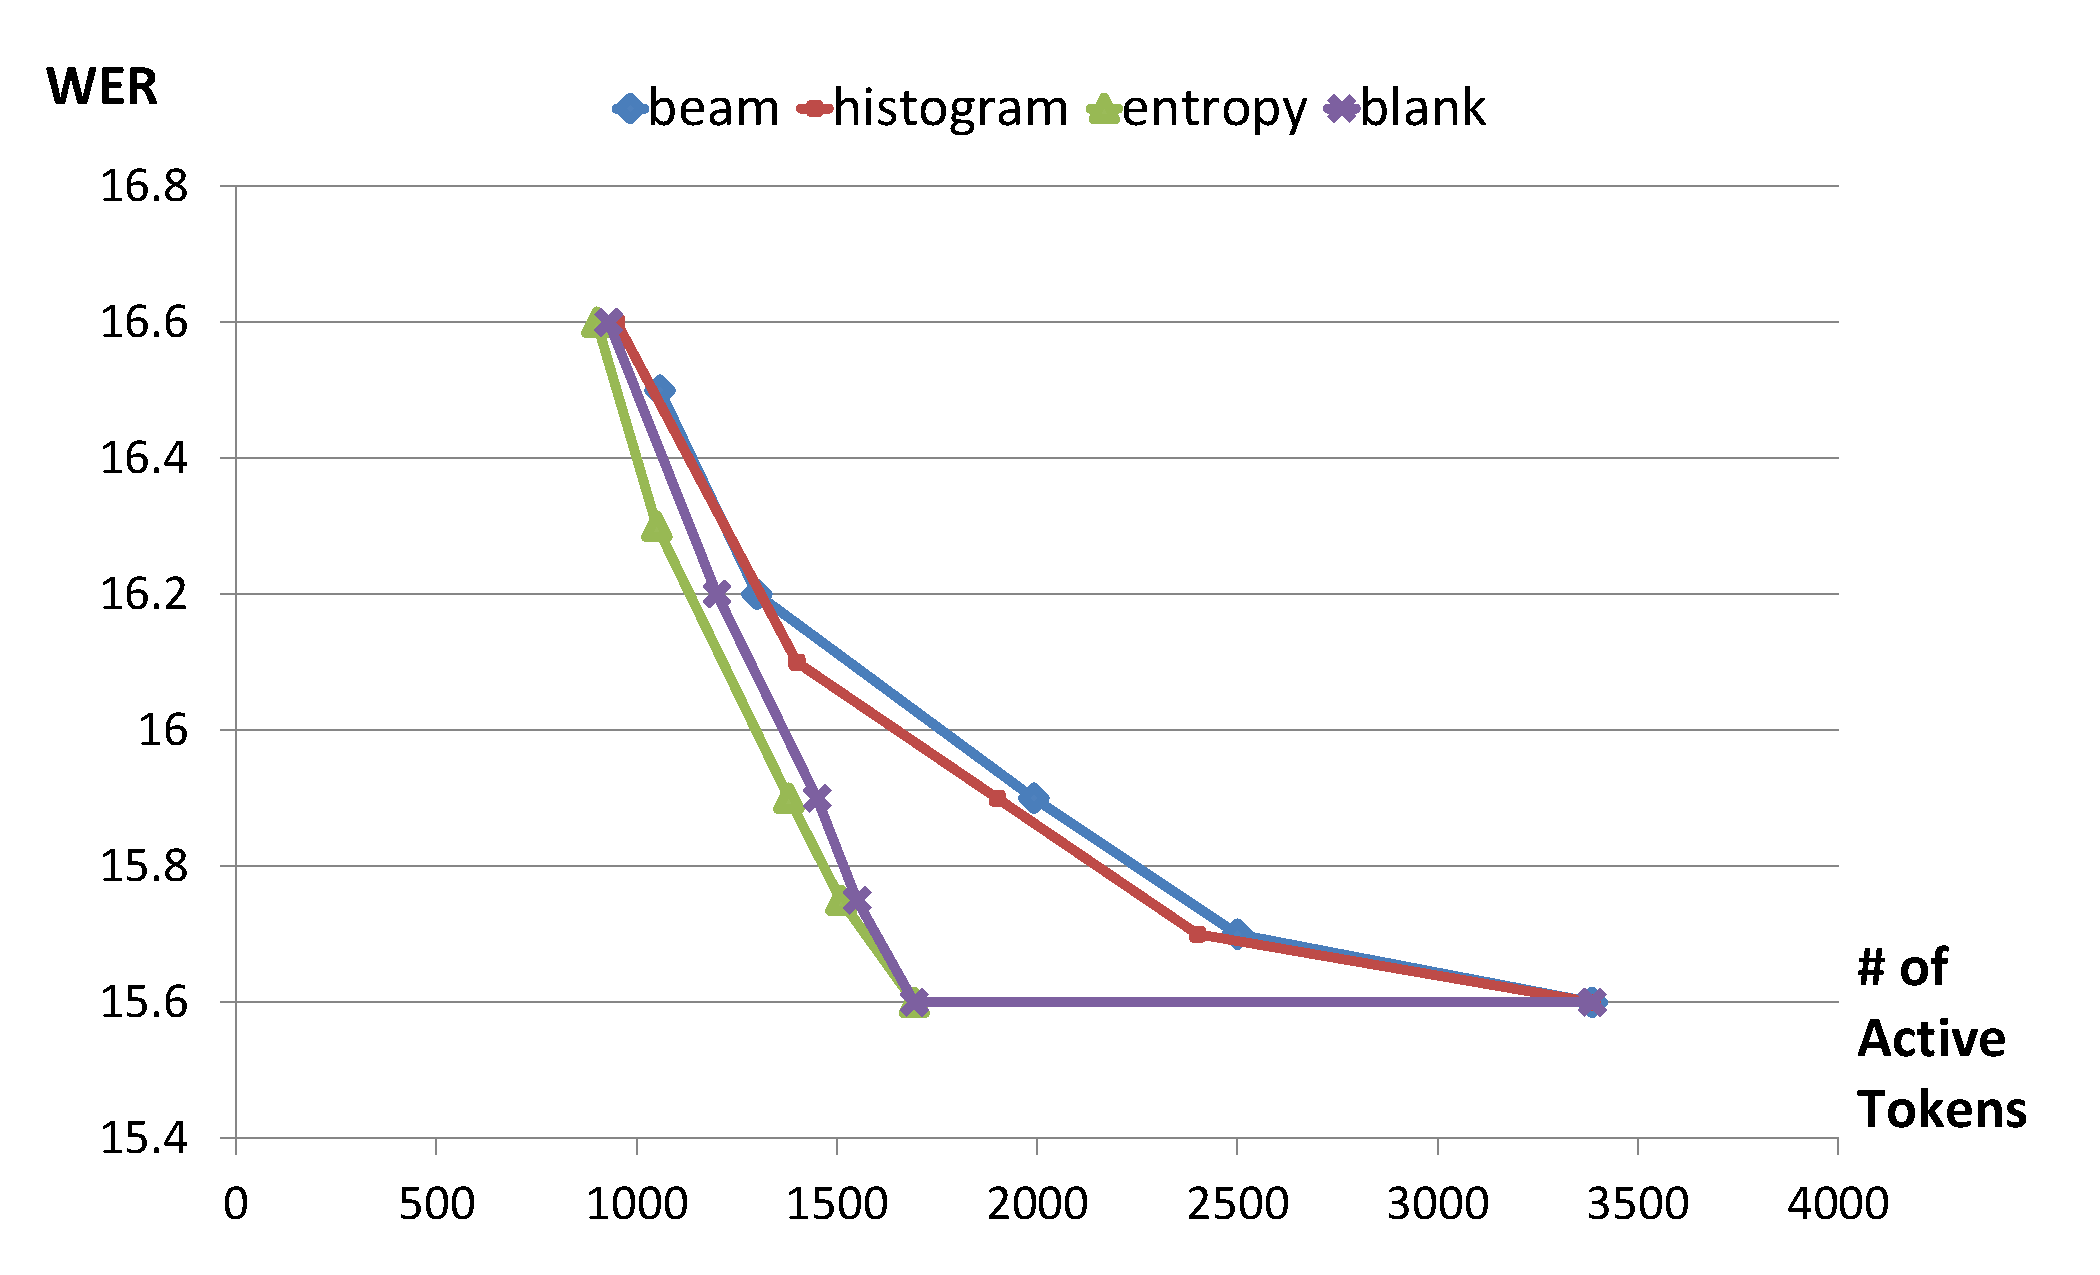
\includegraphics[width=0.8\textwidth]{figure/prune-wer-at-gsm.pdf}
    \bicaption[fig:prune-wer-at-gsm]{LF-MMI中,使用不同剪枝技术时WER随平均活跃令牌数的变化趋势}{LF-MMI中,使用不同剪枝技术时WER随平均活跃令牌数的变化趋势}{Fig}{The trend of WER v.s. the number of active tokens using different pruning methods in LF-MMI.}
\end{figure}

   
(3)进一步设计:本节将对比前文中讨论的各种HMM状态转移模型,以及由此获得的效率的进一步提高。该部分所有实验均在LF-MMI准则上进行,但实验结论可以扩展到其它神经网络和训练准则上。 


     \begin{table}[thbp!]
        \caption{\label{tab:exp-blk-gran-gsm} {\it 生成式序列模型中的blank粒度}}
        \centerline{
    \begin{tabular}{ m{0.1\columnwidth} |m {0.15\columnwidth} ||m {0.06\columnwidth} m {0.06\columnwidth} |m {0.06\columnwidth} m {0.06\columnwidth} m {0.06\columnwidth} m {0.06\columnwidth}}
      \toprule
      \multirow{3}{0.1\columnwidth}{系统}  &
      \multirow{3}{0.15\columnwidth}{$\tt blank$} & 
      \multicolumn{2}{c|}{性能 }& 
      \multicolumn{4}{c}{速度} 
      \\
      &&\multicolumn{2}{c|}{FSD$\mapsto$LSD}&\multicolumn{2}{c}{FSD$\mapsto$LSD}&\multicolumn{2}{c}{FSD$\mapsto$LSD}\\
      &&WER&$\Delta$(\%)&RTF&$\Delta$(\%)&\#AT&$\Delta$(\%)\\
%      \hline \hline
      %\multirow{2}{0.13\columnwidth}{CE} & $\times$ & & & \\
%      \cline{2-5}
%      & $\surd$ & & & \\
%      \hline\hline
      %\multirow{2}{0.15\columnwidth}{sMBR} & $\times$ & & & \\
%      \cline{2-5}
%      & $\surd$ & & & \\
      \midrule
      \multirow{3}{0.15\columnwidth}{TDNN LF-MMI} &  CD phone &15.6 &+1.0&0.13&-43&3386&-45 \\
      & phone &15.7 &+0.9&0.09&-47&2785& -50\\
      % local/chain/run_tdnn_7h_inphone.sh
      % ref: https://spetechcular.com/trac/asr/milestone/report-yby23-2016-11-06
      %local/chain/compare_wer_general.sh tdnn_7h_mhmm_BP_sp
      & global &16.8 &+0.8&0.09&-49&2512& -54 \\
      \bottomrule
%      \hline\hline
      \end{tabular}
        }
    \end{table}

表~\ref{tab:exp-blk-topo-gsm}中列出了不同$\tt blank$粒度的对比结果,即上下文相关的音素$\tt blank$ (CD phone $\tt blank$),音素$\tt blank$ (phone $\tt blank$)和全局$\tt blank$ (global $\tt blank$)。与CD phone $\tt blank$基线相比,phone $\tt blank$在取得近似的解码性能的同时,实现了显著的搜索过程加速;这里搜索加速主要源于较少的模型建模单元,即模型状态数从6K减少到3K。此外,从表中可以看出,global $\tt blank$会带来明显的性能下降;global $\tt blank$需要足够的数据来覆盖不同相邻音素之间的上下文环境(我们认为这也是CTC准则在这个语料库中表现更差的原因之一);CD phone $\tt blank$可以缓解$\tt blank$训练数据不足的问题,但会导致搜索速度变慢;因此,绑定中心音素相同的CD phone $\tt blank$在加速搜索过程的同时,也可以更好地建模$\tt blank$模型;因此,phone $\tt blank$是解码性能和搜索速度之间的最佳平衡。此外,从表\ref{tab:exp-blk-topo-gsm}中可以看出,在LSD框架下,较少的模型单元可以持续带来明显的搜索过程时间缩短:从43\%到 47\%,再到 49\%。最后,phone $\tt blank$是基于LF-MMI的LSD框架的最佳选择。


     \begin{table}[thbp!]
        \caption{\label{tab:exp-blk-topo-gsm} {\it 生成式序列模型中的blank拓扑结构}}
        \centerline{
        \begin{tabular}{ m{0.1\columnwidth} |m {0.1\columnwidth} ||m {0.06\columnwidth} m {0.06\columnwidth} |m {0.06\columnwidth} m {0.06\columnwidth} m {0.06\columnwidth} m {0.06\columnwidth}}
      \toprule
      \multirow{3}{0.1\columnwidth}{测试集}  &
      \multirow{3}{0.1\columnwidth}{拓扑} & 
      \multicolumn{2}{c|}{性能 }& 
      \multicolumn{4}{c}{速度} 
      \\
      &&\multicolumn{2}{c|}{FSD$\mapsto$LSD}&\multicolumn{2}{c}{FSD$\mapsto$LSD}&\multicolumn{2}{c}{FSD$\mapsto$LSD}\\
      &&WER&$\Delta$(\%)&RTF&$\Delta$(\%)&\#AT&$\Delta$(\%)\\
%      \hline \hline
      %\multirow{2}{0.13\columnwidth}{CE} & $\times$ & & & \\
%      \cline{2-5}
%      & $\surd$ & & & \\
%      \hline\hline
      %\multirow{2}{0.15\columnwidth}{sMBR} & $\times$ & & & \\
%      \cline{2-5}
%      & $\surd$ & & & \\
      \midrule
      % https://spetechcular.com/trac/aid201501/wiki/20161011lfmmi-research#modifyHMM
      \multirow{3}{0.15\columnwidth}{TDNN LF-MMI} &  PB &15.6 &+1.0&0.13&-43&3386&-45  \\
      & BP & 15.6 &+1.0&0.13&-46&3392&-49 \\
      %sharper than BPgB
      %& gBPB & 10.4&+1.0&&&& \\
      & BPB & 15.6 &+1.0&0.13&-47&3388&-51 \\
      \bottomrule
%      \hline\hline
      \end{tabular}
        }
    \end{table}

表\ref{tab:exp-blk-topo-gsm}对比了前文提出的不同HMM拓扑结构。在FSD框架下,所有拓扑结构都有相似的解码结果和相同的搜索速度。对比前两行可以看出,与基线PB拓扑结构相比,在LSD框架下, BP可以获得更大的搜索加速。我们认为这个更优的搜索加速源于标签延迟现象,类似于文献\cite{amodei2015deep}中观察到的现象,这使得模型能更可靠地推断标签输出状态并减少混淆。因此,这能带来更尖锐的输出分布。从表中还可以看出,BPB拓扑结构可以进一步改善搜素速度;一些解码路径的例子也表明这种拓扑结构可以使每个上下文相关的隐马尔科夫模型输出更多的$\tt blank$状态。最后,与前面表中CTC的结果相比,LF-MMI中LSD框架能减少49\%的搜索时间。


\subsection{音素级词图质量分析}
\label{sec:exp-lsd-lat-quality}

第\ref{chap:lsd-lsd-lattice}章节中我们提出了LSD音素词图,下面我们将以上述的CTC实验系统为例,对其质量进行验证。
%
%Then, the compactness and precision of phone lattices from different frameworks were compared.
{\em 全局最优音素错误率} (OPER) 被用来对音素词图的质量进行评估。它使用词图中最优的一条路径计算得到的错误率来作为全局错误率\cite{hoffmeister2006frame}。 {\em 词图密度} (Arcs/Sec) 则被用来衡量词图的紧致程度\cite{woodland1994large}。


\begin{figure}[!htp]
  \centering
    \captionstyle{\centering}
    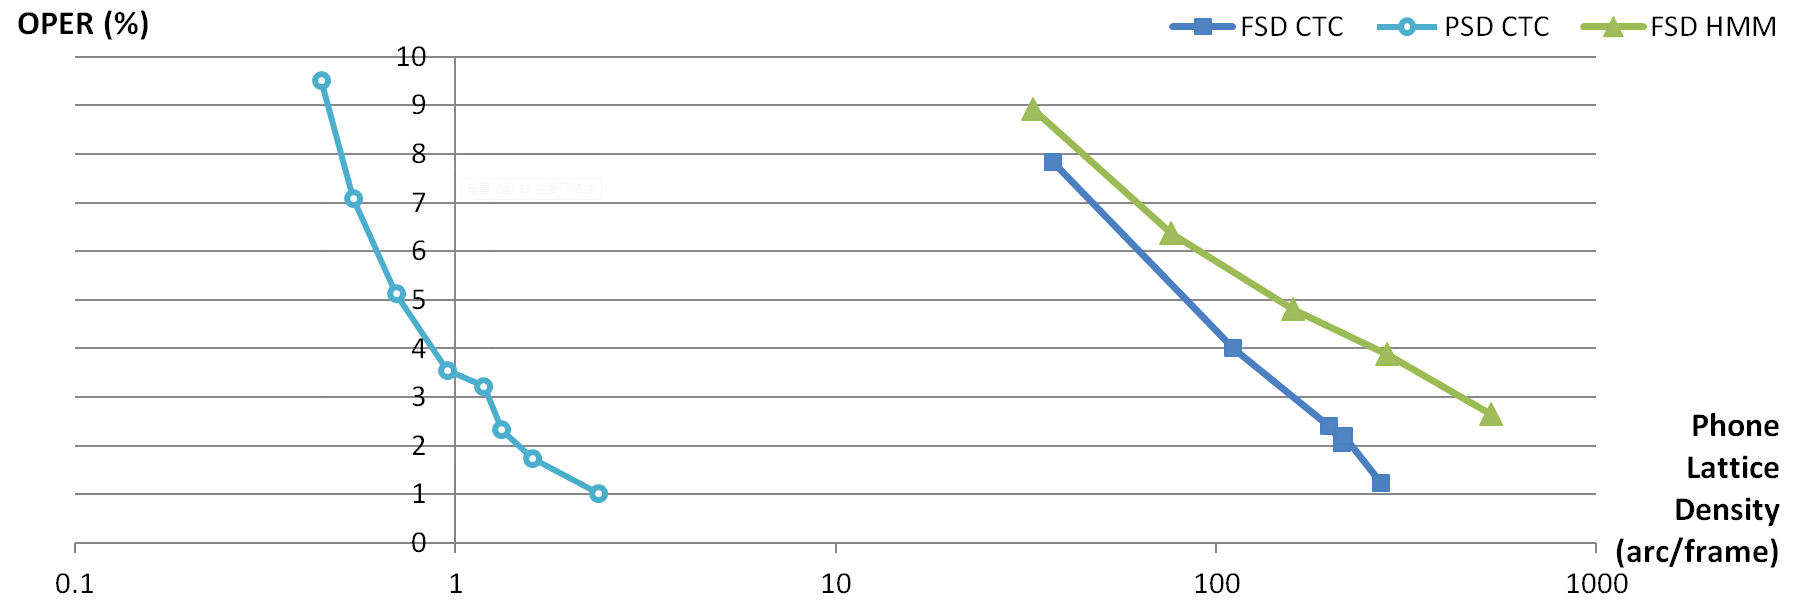
\includegraphics[width=\textwidth]{figure/OPER-latden.png}
    \bicaption[fig:OPER-latden]{OPER v.s. 词图密度在 FSD 和 LSD 中的比较}{OPER v.s. 词图密度在 FSD 和 LSD 中的比较}{Fig}{OPER v.s. lattice density in FSD and LSD}
\end{figure}


图~\ref{fig:OPER-latden}表示了 OPER 和词图密度在不同解码配置结果中的对比,这包括由FSD和LSD生成的音素词图。
%Phone lattice generated from LSD is called LSD CTC lattice as in Section~\ref{sec:psd-ctc-lat} . Phone lattice generated from FSD is as the traditional method \cite{povey2012generating}.
在相似OPER情况下,对同一个CTC模型,LSD词图的大小比FSD词图小超过10倍。而LSD词图比HMM-DNN缩小的数量更大。产生这样现象的原因包括两方面:CTC更突出的后验概率特性而得到的紧致词图;LSD避免了词图生成过程的大量 $\tt blank$ 帧,而FSD则需要进行一些近似 \cite{ljolje1999efficient} 或进行词图裁剪\cite{povey2012generating}, 这将导致更大的搜索误差。
总结起来,在相同大小下,LSD CTC包含更多的音素声学信息。由于接下来的重点是比较FSD和LSD,因此我们仅罗列该部分结果。


%CTC model encodes the many-to-one function of $\mathcal{B}$ and results in peaky phonemic inference results.
%However, in FSD designed for HMM framework, phonemic output lasts for several frames because of  HMM modeling and state transition.  During generating word lattice, many-to-one function still needs to be done by merging same labels with similar time boundary but in a heuristic method (e.g. word lattice pruning).

基于音素级词图,我们可以进一步生成词级词图。 图~\ref{fig:OWER-latden} 表示了词级词图质量在FSD和LSD中的对比。
我们使用OWER进行比较。在图中纵轴,我们画出了 $1-\frac{OWER}{WER}$ 的值作为OWER相对下降值,以体现词图对最终质量改善的上限。从图中可以看出,在相同词图密度情况下,LSD系统总是得到更好的OWER。


\begin{figure}[!htp]
  \centering
    \captionstyle{\centering}
    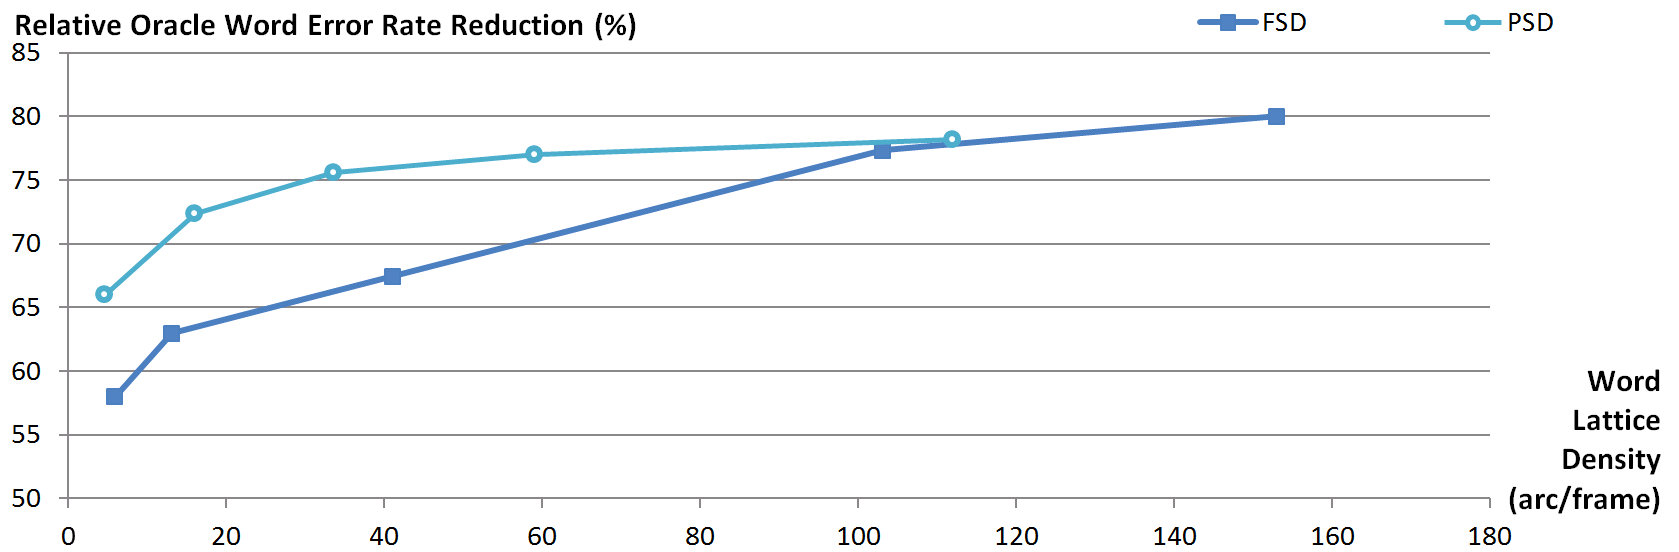
\includegraphics[width=\textwidth]{figure/OWER-latden.png}
    \bicaption[fig:OWER-latden]{词图密度 v.s. 相对 OWER下降比例}{词图密度 v.s. 相对 OWER下降比例}{Fig}{Lattice density v.s. rel. OWER reduction}
\end{figure}

基于上述质量更好的音素级词图和词级词图,在下一章节中,我们将具体介绍LSD音素词图的各种扩展应用。

\section{本章小结}
\label{chap:lsd-sum}

在本章中,我们针对语音识别和端到端建模的推理搜索阶段,提出了标签同步解码算法,其通过一系列方法使得搜索解码过程从逐帧同步变为标签同步,这包括使用高效的$\tt blank$结构和后处理方法。该文提出的一系列通用方法在隐马尔科夫模型和连接时序分类模型上得到了验证。同时该章节还介绍了将标签同步算法应用于序列到序列的端到端模型的方案。在实验部分,该章节系统取得了大幅度语音识别解码速度改善。


\chapter{基于标签同步解码的统一解码框架}
\label{chap:unify}

由于不同ASR应用之间不同的搜索空间大小和效率要求,当前业界最优的置信度及其相应的解码算法在不同应用上具有不同架构,这些不同应用包括:关键词检测,基于上下文的语音识别和大词汇连续语音识别。针对基于词图后验概率的置信度,计算量主要集中在词图部分的边缘概率计算过程。本章节中,我们将结合前面章节对解码的大幅加速和搜索空间的优化等工作,提出一系列针对不同应用的通用置信度,并尝试将不同应用中的语音识别推理过程统一到同一框架中。

\section{基于标签同步解码的置信度框架}
\label{chap:unify-confidence}


连接时序分类模型 (CTC) 是一种目前比较主流的LVCSR模型。但是由于 $\tt blank$ 的引入,使得基于 CTC的词语级别的置信度 (CM) 并不能够被直接得到,特别是最主流的针对传统基于音素似然度归一化或者基于词图后验概率的混淆网络等方法。
在前文中我们提出了标签同步解码(LSD)的推理框架,它的主要作用是针对CTC或HMM模型进行高效的解码搜索。该算法提出了一些方式来自动地将 $\tt blank$ 帧进行忽略,由此不仅得到了搜索上的加速,还得到了一种非常紧致高效的 CTC 音素词图。在这项工作中,两种置信度生成算法在标签同步解码算法的基础上被提出。
更细致的研究显示这种基于CTC的音素词图是得到更好性能的关键所在。
在英文Switchboard 上的大词汇连续语音识别任务显示这里提出的LSD CTC 词图置信度算法可以显著改善原先传统的基于逐帧解码算法的CTC置信度或者 HMM模型的置信度。

\subsection{引文}
\label{sec:intro}

% TODO: ref http://hci.stanford.edu/research/speech/
在最近十年时间,自动语音识别 (ASR) 取得了非常显著的成功。但是当语音识别系统由实验室产品转向真正的应用时,即使是最好的语音识别系统,仍然会不可避免地产生一些识别中的错误 \cite{ruan2016speech},也就是说ASR系统的输出总会包含或多或少的一些各种各样的错误。
因此,在真实的应用场景中,人们一般需要ASR系统能够自动评估自身的可靠性和发生错误的概率,而这些都由系统自身得出。

在语音识别中,置信度(CM)就是提出来进行这种类型的可靠度评估的\cite{jiang2005confidence}。这类模型可以被分为如下几种类别:

\begin{itemize}
    \item {\em 基于用于建模的特征的置信度}.
    基于ASR识别过程的特征被称为用于建模的特征,而它的概率分布在识别正确和识别错误时会产生显著的不同。
    CM可以由它们之中的一个或两个来组成,比如对归一化后的声学分数 \cite{hu2013new}, 时长 \cite{ma2011fusing}, 局部交叉熵 \cite{falavigna2002acoustic}。
    但是,这些用于建模的特征并不完美地表示解码的过程 \cite{jiang2005confidence}. 所以一些分类器模型也可以考虑被加入到这些用于建模的特征上,比如 CRF \cite{seigel2013confidence}, 深度学习 \cite{yu2011calibration}, 等等。但是这些模型仍然不够完美。首先各个用于建模的特征之间并不完全独立,其次它需要额外的训练阶段,并假设训练数据与测试数据匹配。
    %feature and model method weakness:
    %need further training stage; hard to formulate; depend on scenario of training data, assuming scenario of test and training data is the same

    \item {\em 基于后验概率的置信度}.
    另一种方法将ASR过程建模为 {\em 最大后验概率} (MAP) 的决策过程。给定整个句子后的ASR输出的后验概率可以用来表示CM。许多方法研究了如何对归一化项进行建模,比如 filler 模型 \cite{young1994detecting}, 词图\cite{wessel2001confidence} 和混淆网络 \cite{evermann2000large}。然而,ASR解码器通常设计用于寻找最优的首选路径,这使得它所得到的词图并不完美,同时会导致CM的建模并未较好地归一化 \cite{yu2006maximum}.
    %filler/lattice/cn

\end{itemize}

%review CTC & LSD & its potential in CM
CTC\cite{graves2006connectionist} 被提出来并作为目前主流的新模型\cite{fernandez2008phoneme}\cite{sainath2015acoustic}\cite{amodei2015deep}\cite{sak2015fast}.
同时,上下文无关的单音素CTC也显示出非常有竞争力的性能,在相比传统上下文相关的聚类混合深度学习HMM模型\cite{sak2015fast}\cite{miao2015eesen}\cite{miao2016ctc}\cite{mcgraw2016personalized}的情况下。
然而,由于引入了$\tt blank$, CM的计算亟待研究。如本文的实验部分所示,如果只是将 $\tt blank$ 标签当做一个特殊的音素并使用传统的CM方法,将会引入较大的性能下降。
在前文中我们提出了标签同步解码(LSD)的推理框架。它的主要作用是针对CTC模型进行高效的解码搜索。该算法提出了一些方式来自动地将 $\tt blank$ 帧进行忽略,由此不仅得到了搜索上的加速,还得到了一种非常紧致高效的 CTC音素词图。在这项工作中,两种置信度生成算法在标签同步解码算法的基础上被提出。
更细致的研究显示这种基于CTC的音素词图是得到更好性能的关键所在。
在英文Switchboard 上的大词汇连续语音识别任务显示这里提出的LSD CTC 词图置信度算法可以显著改善原先传统的基于逐帧解码算法的CTC置信度或者 HMM模型的置信度。


\subsection{LSD CTC词图中的置信度}
\label{sec:pp-conf-measure}


\subsubsection{标签同步的音素声学置信度}
\label{sec:psd-ac-conf}

%as local confidence
在前文中,我们已讨论了标签同步解码算法,它的主要作用是针对CTC模型进行高效的解码搜索。该算法提出了一些方式来自动地将 $\tt blank$ 帧进行忽略,由此不仅得到了搜索上的加速,还得到了一种非常紧致高效的 CTC音素词图。
下面我们将集中讨论基于这些 CTC音素词图如何得到较好的置信度。

这里CTC音素后验概率可以依据词语进行区分,属于同一个词的后验概率可以用于一起对一个特定词在词图中出现的后验概率进行建模。
在LSD框架中,词级别的 CM $\mathcal{C}(w)$ 可以被定义为对数域的后验概率,针对其相应的最优路径。
% introduction of phonemic confidence


     \begin{equation}\label{eq:psd-ac-conf1}
        \mathcal{C}(w)  =
         \log\!\!\!\!\!\!\sum_{\bm\pi \in \mathcal{B}^{-1}(\mathbf{l}_w)}{\!\!\!\!\!\!P(\bm\pi|\mathbf{x})}
        \triangleq
   \!\!\!\!\!\!\mathop{\max}\limits
       _{\!\!\!\!\pi':\pi' \in L, \mathcal{B}(\pi'_{\mathbf{j}_w})       =       {\mathbf{l}}_w}
   \sum_{j:j\in \mathbf{j}_w}
   \log({y^{t_{j}}_{\pi'_{j}}})
     \end{equation}

$\mathbf{l}_{w}$ 表示词语  $w$对应的音素序列。
$j$ 是音素序列的索引 (i.e.  \cite{zhc00-chen-tasl2017}中定义的非$\tt blank$ CTC 标签序列).
由于LSD CTC中的词边间比较确定, $\mathbf{j}_w$ 可以被定义为 $w$ 词所最佳对应的音素序列索引。
我们提出的基于标签同步解码的声学分数可以作为单独的置信度,也可以与其他用于建模的特征结合,作为置信度模型的输入 \cite{yu2011calibration}。 
具体来说,$\mathcal{B}$函数的建模在CTC中并不完美,使得这里会出现同一个音素有多帧的音素后验概率输出。所以,我们需要在它上面进一步进行归一化。 其中一种方法是进行算数平均,被称为 {\em peak-mean}。但是,由于有多个概率输出尖峰,更好的一种方法是忽略不完美的部分并保留最大的结果,所以从中挑选最大的后验概率作为其置信度,被称为 {\em peak-max}。除此之外,不同词语具有不同的长度,因此我们需要针对长度作一次平均。为了使性能更好,我们这里对音素序列的长度也进行了归一化 称为{\em phone-mean}。

% introducing (no blk) confidence
另一类比较现实的问题是, {$\tt blank$} 的区段和音素区段有所重合。因此这里需要对非$\tt blank$的概率同样进行一些建模。音素置信度 (称为 {\em phone-conf }) 可以被定义为某帧上输出音素标签的概率。
%, in proposed CM (\ref{eq:psd-ac-conf1})
% \begin{equation}\label{eq:nblk-conf}
%    P( \tt phone^{t} |\mathbf{x}) = 1-y^{t}_{\tt{blank}}
%     \end{equation}
以上这些针对不同模块的设计总结如下 (\ref{eq:psd-ac-conf2}),

     \begin{equation}\label{eq:psd-ac-conf2}
        \mathcal{C}(w)
        \triangleq
        \!\!\!\!\!\!\mathop{\max}\limits
       _{\!\!\!\!\pi':\pi' \in L, \mathcal{B}(\pi'_{\mathbf{j}_w})       =       {\mathbf{l}}_w}
   \frac{1}{|\mathbf{j}_w|}\sum_{j:j\in \mathbf{j}_w}
   \max_{t:t\in\mathbf{t}_j}
   {\log(y^{t}_{\pi'_{j}}(1-y^{t}_{\tt{blank}})^\alpha)}
     \end{equation}
这里的 {\em peak-max} 作为一个例子出现在公式中。 $\mathbf{t}_j$ 是音素 $j$ 在最优路径下所相应的帧。 $\alpha$ 是置信度融合的权重概率。

%  \begin{equation}\label{eq:psd-ac-conf2}
%        CM(w)
%        =
%   PN(FN(\mathbf{t}_j,y\cdot(1-y_{\tt{blank}})),\mathbf{j}_w)
%     \end{equation}

\subsubsection{基于混淆网络和CTC标签同步解码词图的置信度}
\label{sec:psd-cn-conf}

类似于 \cite{evermann2000large}中的做法,这里生成混淆网络主要有两步: a) 从音素级别的标签同步CTC音素词图(图~\ref{fig:ctc-lat-exp})中产生词级词图; b) 将词级词图转换为混淆网络,利用其包含的时间边界信息。在 \cite{hakkani2006beyond}中提出的 pivot clustering 算法使得混淆网络生成复杂度为 $O(n)$ , $n$ 为词图的边数。在这项工作中,我们将最优路径视为pivot, 由于CTC词图非常紧致,因此  CN 产生的过程非常高效。在CN的构建过程中, 我们需要计算词后验概率,而其自然地成为了词级置信度。



\begin{figure}[tbhp!]
        \centering
        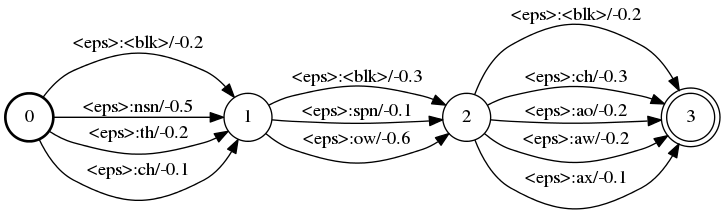
\includegraphics[width=0.95\linewidth]{figure/ctc_lat.png}
        \caption{{\it  LSD CTC Lattice的例子}}
        \label{fig:ctc-lat-exp}
      \end{figure}

图~\ref{fig:lat-exp} 中是一个真实的例子 (句子为 "OH YEAH") 表示了LSD CTC 产生的CN的高效性,以及与HMM-DNN产生的词图之间的比较。
由HMM和CTC得到的推理结果在图~\ref{fig:lat-exp}(a)中进行显示,其得到的音素词图,词级词图,分别在HMM和CTC系统中展示于图~\ref{fig:lat-exp}(b$\sim$e)中。我们可以观察到,CTC基于LSD得到的音素词图和词级词图比相应的HMM词图更加紧致,这是源于$\mathcal{B}$函数的建模结果。另一方面,HMM的词图需要额外的启发式方法来进行多对一的映射,以便去除词图冗余性。这里的做法是进行词图裁剪 \cite{siniscalchi2013bottom}, 而它不如 $\mathcal{B}$ 函数的效果那么强。
另一方面,当CTC模型被使用于传统的 {\em 逐帧同步解码} (FSD) 框架时, 音素和词级词图可以由同样方法进行产生\cite{povey2012generating},类似于处理 HMM-DNN 词图的方式对 $\tt blank$ 标签进行等同于音素的处理。但是由于逐帧搜索和词图此案件所带来的搜索误差,以及词图边界的混淆性,所得到的CN将会具有更差的质量。我们将会在后续的实验章节中进行详细比较。

%FSD Lattice v.s. LSD Lattice
%
%snt example fig:
%ref word v.s. phn dnn align v.s. phn dnn decode v.s. phn CTC align v.s. phn CTC decode
%v.s. FSD lattice v.s. LSD lattice v.s. CN
%in a single figure

%analysis on latter indicators in experiment part

\begin{figure}[tbhp!]
        \centering
        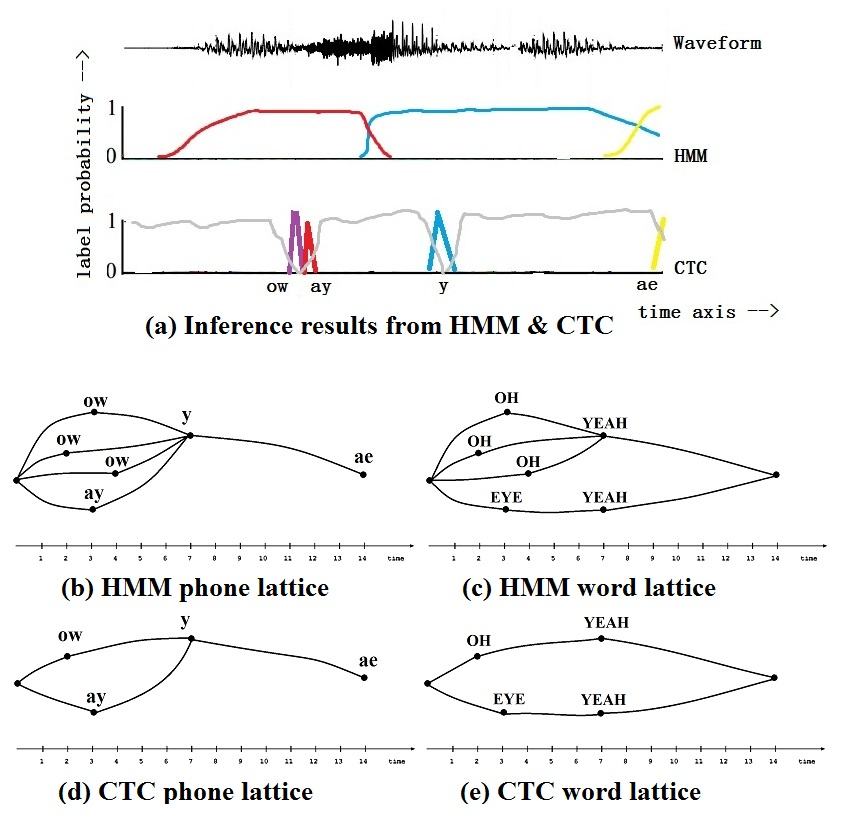
\includegraphics[width=0.95\linewidth]{figure/lat-exp.jpg}
        \caption{{\it FSD HMM 和 LSD CTC所产生的词图比较}}
        \label{fig:lat-exp}
      \end{figure}

\section{基于标签同步解码的多识别任务统一框架}
\label{chap:unify-framework}

要为所有的ASR应用设计一套统一的推理框架,并取得最好的性能和速度,是一项非常有挑战的研究。这里面的关键点在于: i) 如何对最佳识别结果进行规范化,以得到对该最佳结果的置信度估计,也就是置信度中的归一化项的建模
    ii) 如何保证在低功耗设备中的计算量控制在一个较小范围内,比如关键词检测技术就经常被用于个人助理情况,需要对功耗进行优化。
    {\em Keyword-filler}方法~\cite{young1994detecting} 和 {\em utterance verification}~\cite{rose1995training} 方法都可以视为这方面的尝试。比如,在关键词检测中,一些研究提出使用上下文无关的(CI) 语言学单元,称为 $\tt filler$ 来对所有非关键词部分进行建模,而这种建模往往是不完美的。
    在基于上下文的语音识别中,这种框架更加受制于较弱的上下文建模能力,而这将影响 $\tt filler$ 的识别效果。
    %More elaborated $\tt filler$~\cite{el1997accurate}, e.g., CD $\tt filler$, is proposed to improve the recognition but brings about further computational burden without significant improvement.
    在LVCSR中,理论上更好的办法是基于识别结果的后验概率方法的置信度~\cite{wessel2001confidence}, 也就是前文讨论的第二种置信度。 在这种置信度里,ASR被建模为  {\em maximum a posterior} (MAP) 过程:给定句子,求取当前识别结果的后验概率,并将其作为置信度。而这里的观察概率(归一化项)使用针对搜索空间的所有可能候选概率求和来得到。由于ASR搜索空间很大,词图建模很耗时。在LVCSR中,这种框架往往取得最好的效果,但在其他任务中结论不尽相同。

    最近在鉴别性训练领域,有些研究采用一个特别设计的音素语言模型作为搜索空间来代替词图,该方法显示出了较好的性能~\cite{chen2006advances}\cite{povey2016purely}。受次启发,我们尝试将这样的音素语言模型应用到置信度的归一化项的建模当中,由此我们提出了辅助归一化搜索空间的概念。我们尝试使用这样的搜索空间来建模所有ASR应用领域的置信度。 % and CM can be obtained in an unified framework
    而针对这样做在低功耗设备上带来的挑战,我们采用基于CTC的标签同步解码\cite{Chen+2016} 来进行处理,由此带来了很大的效率改善。
    由此我们提出了一个统一并且高效的置信度框架,并且将其应用于目前主流的上述三种 ASR应用。

  \subsection{置信度和搜索空间}
  \label{Sec:conf-search-space}

  关于搜索空间和解码框架的不同,通常可以根据不同ASR应用将其分为三类,而三种应用上目前最好的置信度算法方式并不统一。

  \subsubsection{关键词检测}
    \label{Sec:kws-task}

    	关键词检测任务目标是准确和快速地检测语音中是否包含所关心的词或短语。所以,关键词检测的搜索空间是所有的关键词序列~\footnote{基于大词汇连续语音识别的关键词检测目前并不包含在讨论中,因为这类方法主要研究在于如何提高声学模型性能以及关键词索引技术。同时计算量过大也不适合端侧设备。}。 误接收表示错误地将某些语音段识别为关键词,而这并不是希望得到的。一系列研究~\cite{young1994detecting,chen2014small}尝试解决这样的问题,包括使用一定阈值进行后处理估计,或将Filler加入声学建模中。

  \subsubsection{基于上下文的语音识别}
  \label{Sec:task-task}

  针对语音助手等应用,目前对于基于上下文的语音识别的需求越来越强。在这些场景中,语法~\cite{woodland1994large} 或基于类的语言模型~\cite{ward1996class} 都是比较主流方法~\cite{vasserman2016contextual}。
  这种任务的错误识别包括:i) 错误将领域外的句子识别为领域内的结果 ii) 正确识别出了领域,但是上下文短语的部分识别错误。为了给出合理的结果,置信度用于对识别结果进行判别。对于领域内识别,语音模式和上下文信息识别可以被看做是一个完整的搜索空间,这时使用LVCSR的后验概率的置信度是合理的。但是对于领域外的句子,上面提到的置信度并没有对其搜索空间进行建模。因此这样的置信度目前还没有比较合理的方案进行解决。

  \subsubsection{大词汇连续语音识别}
  \label{Sec:lvcsr-task}

  在 {\em 大词汇连续语音识别} (LVCSR)~\cite{woodland1994large}中,  搜索空间由N元语言模型进行建模。为了支持语言学后处理~\cite{hakkani2006beyond}, CM被用来提供对语音识别结果的可靠度分析。
  基于识别结果后验概率的CM~\cite{wessel2001confidence}是LVCSR中最通用的置信度方法。
  在这一框架中,ASR使用 {\em maximum a posterior} (MAP) 决策过程进行建模。给定整个特征序列的ASR输出的后验概率被作为句子的置信度。 对于MAP的归一化项,即观察概率建模,使用的是所有识别结果组成的搜索空间的后验概率求和。由于语音识别的搜索空间很大,通常这一过程由解码得到的词图来进行限制。

  \subsection{基于附属归一化搜索空间的置信度方法}
  \label{Sec:norm-gragh}

这篇文章里,我们尝试提出一个能够适用于各种ASR应用的统一框架。我们的方案基于所提出的附属归一化搜索空间和基于CTC的标签同步解码方法。

  \subsubsection{统一的置信度框架}
  %\subsubsection{Hypothesis Posterior based Confidence Measure}
  对于ASR输出的后验概率可以在MAP框架中作为一个句子级别的置信度。
  \begin{equation}\label{eq:cm-post}
        CM=P(\mathbf{w}|\mathbf{x}) =
         \frac{P(\mathbf{x}|\mathbf{w})\cdot P(\mathbf{w})}{P(\mathbf{x})}
  \end{equation}
 公式中 $P(\mathbf{w})$表示语言模型概率 $P(\mathbf{x}|\mathbf{w})$  是声学模型的部分。 $P(\mathbf{x})$ 是观察概率 $\mathbf{x}$ , 由下式建模,
   \begin{equation}\label{eq:cm-obser}
        P(\mathbf{x})=\sum_H P(\mathbf{x},H)= \sum_H P(H) \cdot  P(\mathbf{x}|H)
  \end{equation}
 这里$H$ 表示所有可能的识别结果的路径。 $H$ 根据不同的ASR应用而有所不同。因此 $H$ 的建模通常都是性能的瓶颈。

构建这样的通用框架的主要挑战在于:i) 如何对任务相关的集合 $H$使用一个统一框架进行建模 ii) 如何在计算效率较高的情况下对无限的$H$进行建模。
 %Besides, ASR decoders are commonly designed for finding the single best path, which results in imperfect word lattice and leads to unnormalized posteriors in CM.


 \subsubsection{附属归一化搜索空间}
 \label{Sec:norm-graph-detail}

 %lattice-free method
 为了解决这个问题,我们提出使用附属归一化搜索空间,将其作为归一化项的搜索空间进行建模。该方法的框架图~\ref{fig:graph-example}所示。 

 在基于词图的方法中,$P(\mathbf{x})$ 是从解码网络的一个子区域,词图中进行计算的。在基于 $\tt filler$ 的方法中, $P(\mathbf{x})$ 是由自环的音素组成的。在我们所提出的方法中 $P(\mathbf{x})$ 由下述的搜索空间得到
 \begin{equation}\label{eq:cm-obser2}
 P(\mathbf{x})\approx \max_H P(H) \cdot  P(\mathbf{x}|H)
 \end{equation}
 这里,我们尝试了三种不同的附属归一化搜索空间。
 \begin{itemize}
     \item 自环音素搜索空间 ($\tt AX1$). 类似于传统的关键词-filler置信度\cite{young1994detecting},  一个由所有的音素组成的网络可以用来建模归一化项的边缘概率值。
     %Traditional filler based CM directly models observation probability without  lattice.

     \item 无词典搜索空间 ($\tt AX2 $). 受到近期无词图鉴别性训练方式的启发~\cite{povey2016purely},  附属归一化搜索空间可以由一个音素级语言模型而得到,用于近似搜索空间。
         %when calculating CM, the LM score is not counted in.

     \item 基于词典的搜索空间 ($\tt AX3 $). 在一些语言当中,比如汉语,音频与字符的关系是多对一映射的 \footnote{而像英语,这个映射是多对多}. 所以,在给定相对固定数量的字符后,我们可以预期的发音数量是有限的。所有可能的发音可以作为一个附属归一化搜索空间。
 \end{itemize}
 除此之外,我们所提出的方法可以作为词级别的置信度。这种情况下公式(\ref{eq:cm-post}) 和 (\ref{eq:cm-obser2}) 可以被转化为公式(\ref{eq:cm-post3}) 和 (\ref{eq:cm-obser3}),

 \begin{equation}\label{eq:cm-post3}
        CM=P(w|\mathbf{x}) =
         \frac{P(\mathbf{x}|w)\cdot P(w)}{P(\mathbf{x}^{w})}
  \end{equation}
 \begin{equation}\label{eq:cm-obser3}
 P(\mathbf{x}^{w})\approx \max_{H^{w}} P(H^{w}) \cdot  P(\mathbf{x}^{w}|H^{w})
 \end{equation}
 
 附属归一化搜索空间的解码结果是对观察概率的一个很好估计。由于声学模型的单元通常是音素,这样的置信度框架在大多数语音识别应用中都是合适的。与传统词图方法相比较,这里提出的方法相比其他的ASR搜索空间更加稳定鲁棒,我们将在实验中证实这一点。除此之外,这套方法不需要再额外引入一系列非关键词的模型建模单元,比如基于 $\tt filler$ 或者语句验证这类估计框架。
 所以, 置信度归一化建模可以是相对原始搜索空间和声学模型而独立的部分。

 \begin{figure}[tb]
        \centering
        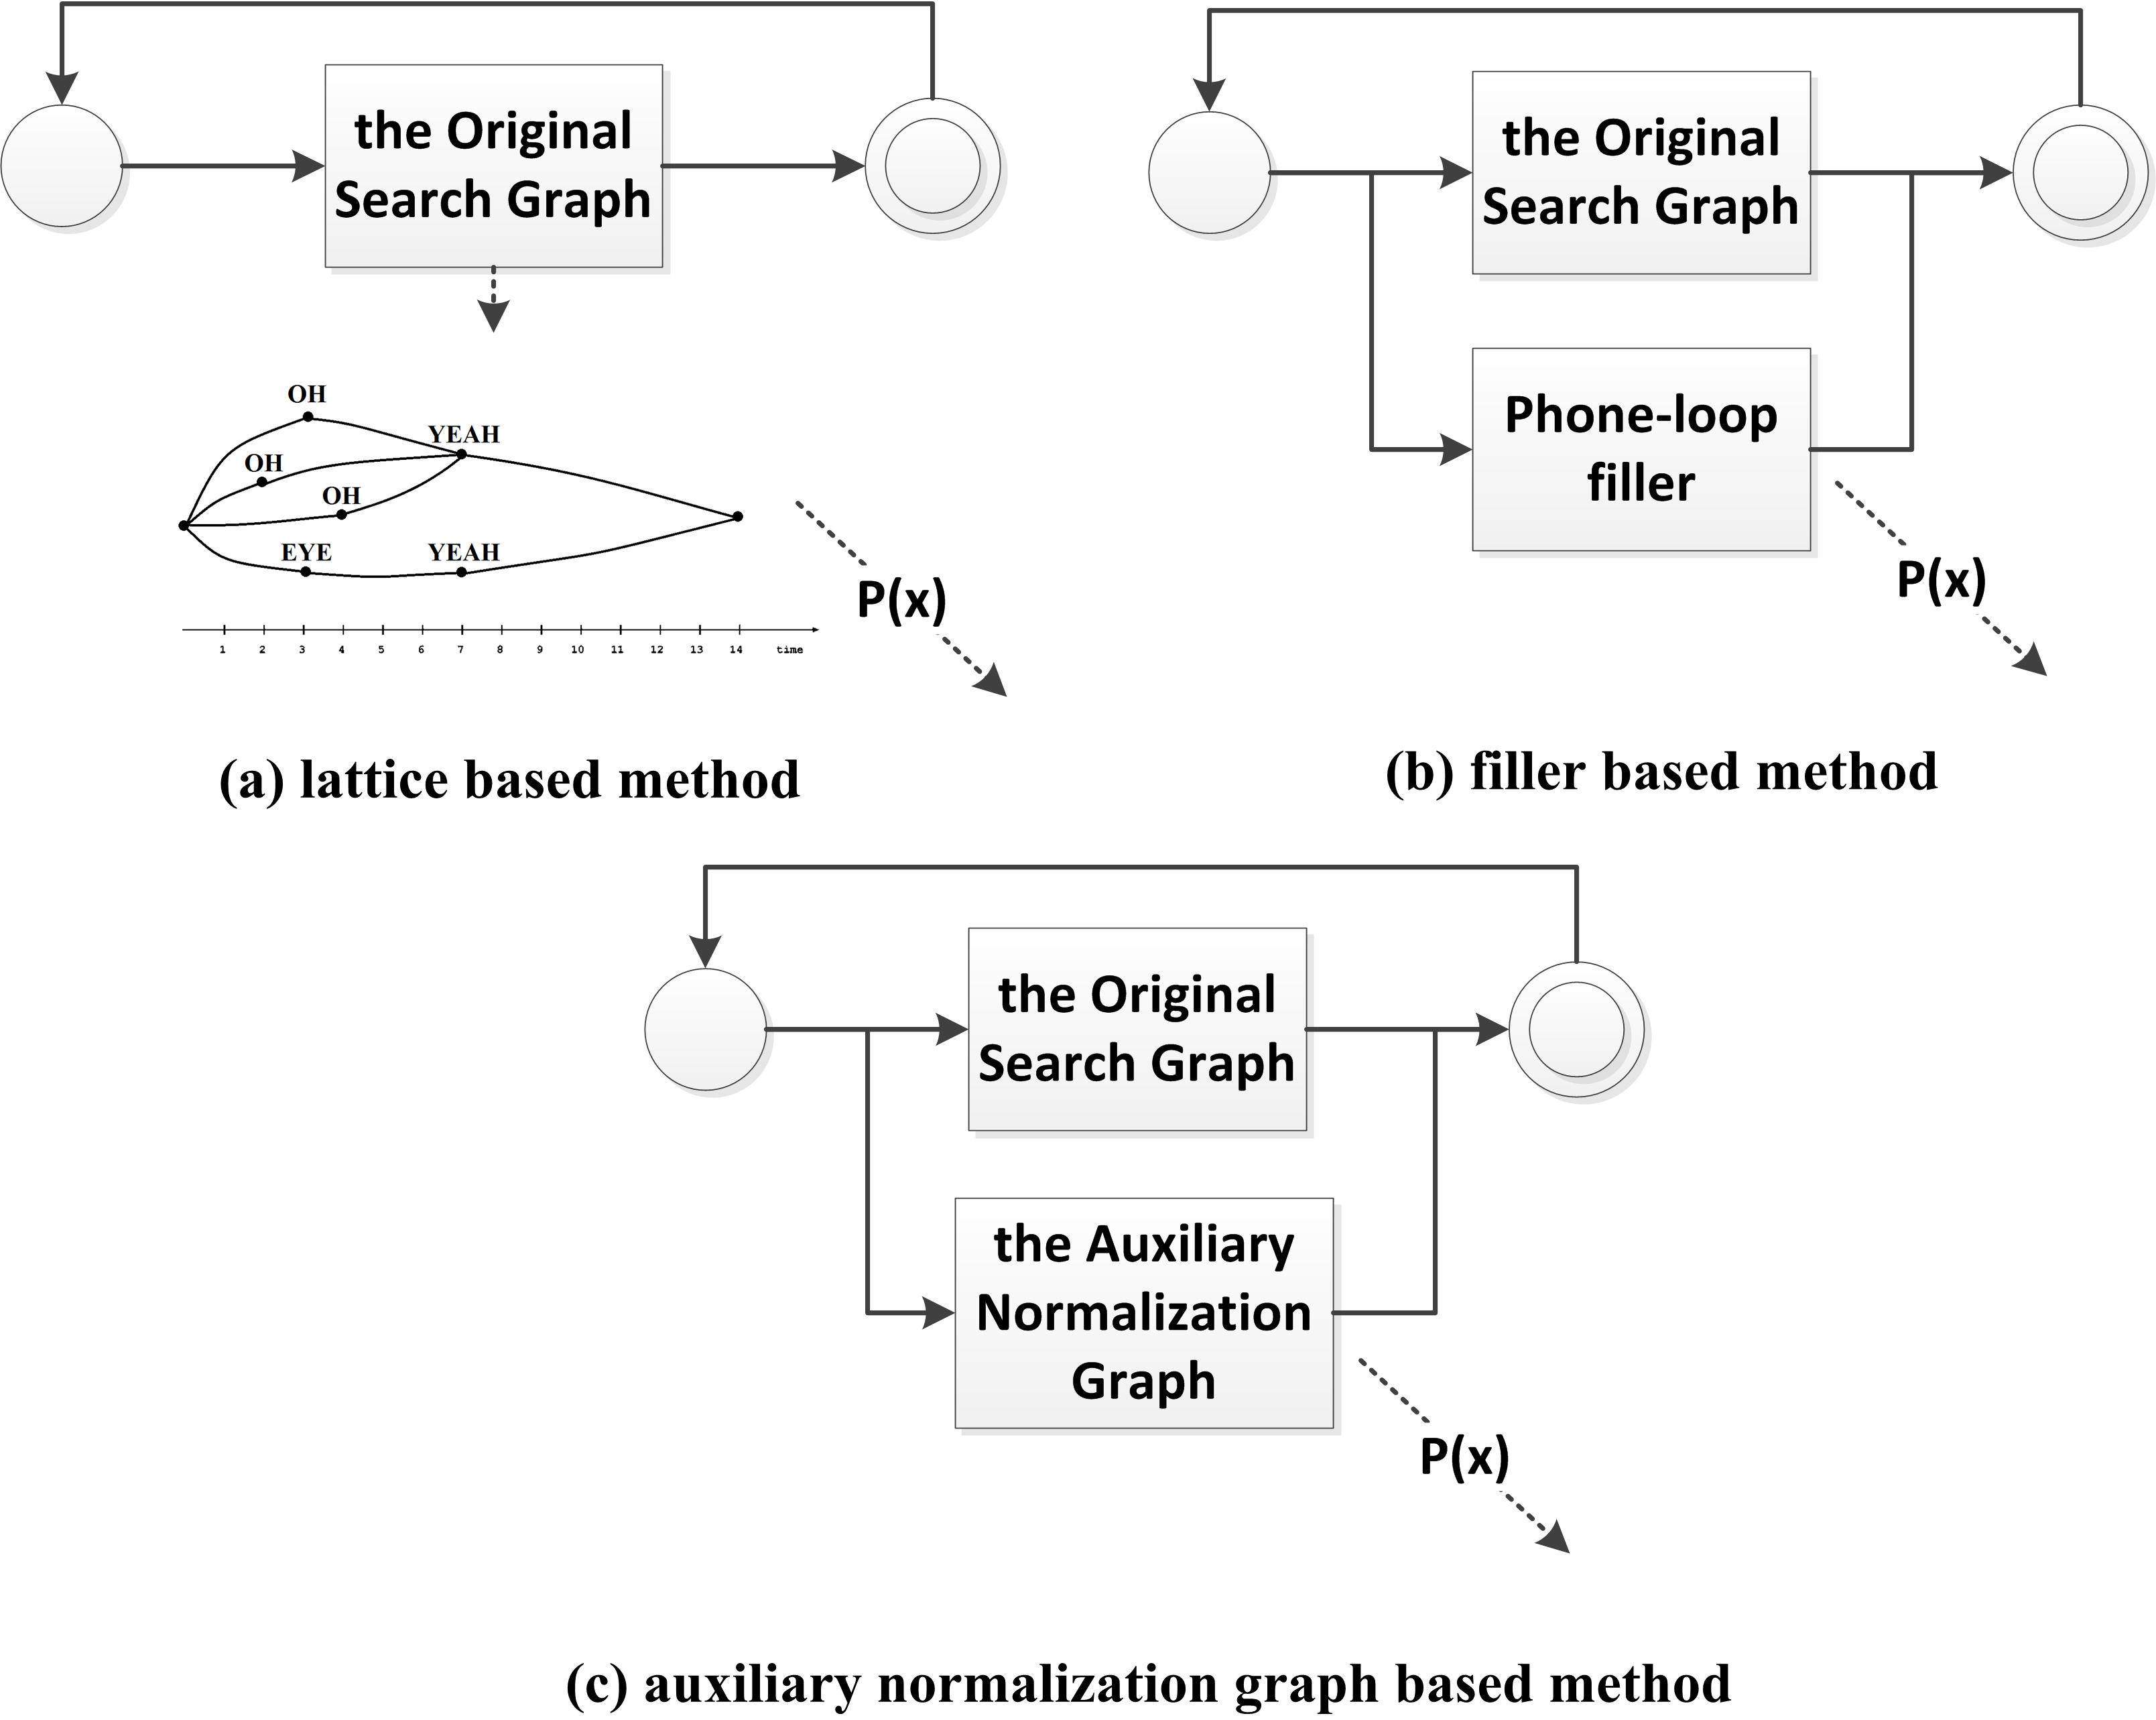
\includegraphics[width=0.7\linewidth]{figure/graph_example.png}
        \caption{{\it 架构比较。这里原始的搜索空间包括,关键词检测,基于上下文的语音识别,和大词汇连续语音识别。 }}
        \label{fig:graph-example}
\end{figure}

 \subsubsection{基于CTC的标签同步解码}
 \label{Sec:psd-ctc}

上面讨论的方法具有一定的计算昂贵性,特别是针对低功耗应用比如关键词检测。基于CTC的标签同步解码 \cite{Chen+2016} 可以考虑被采用,以加速这样的应用。由于这类方法可以跳过blank的区段,使得结果中具有更少的混淆,这体现在公式 (\ref{eq:cm-obser})中。这类方法也被前面的章节证明,解码只占全部计算量的一小部分 \cite{Chen+2016}\cite{zhc00-chen-tasl2017} 。在实验中我们将验证相关结论。


\section{实验结果}
\label{chap:unify-exp}


\subsection{实验配置}

%In this section,  phone lattices from FSD and LSD were firstly compared, and their effects on CM were analyzed. Then experiments were held on proposed two types of CMs.

%\subsection{Experimental Setup}
%\subsubsection{Setups and Evaluation Metrics}

%%%%%%%%%%%% CM %%%%%%%%%%%%%
我们的置信度实验主要在300小时Switchboard上进行。而针对多种任务的融合框架则在后面介绍。
我们训练得到了上下文相关的状态级别HMM (CD-state-HMM) 和上下文无关的音素级别CTC (CI-phone-CTC) 。 训练的配置与解码配置和上文相似  \cite{zhc00-chen-tasl2017}。
所有的模型都使用大约 2-2.5M 参数,以便进行公平比较。
在测试中, 我们使用NIST Hub5e00 测试集的switchboard子集 (1831 句子) 。对CTC模型,我们测试FSD和LSD两种方法。
表~\ref{tab:asr-baseline} 给出了不同模型和解码框架下的基础性能,其与前文保持一致。



    \begin{table}[th]

    \caption{\label{tab:asr-baseline} {\it WER 比较}}
        \centerline{
          \begin{tabular}{ c  c  c  || c }
            \hline
            {Model Unit} &
            AM &%\multicolumn{1}{|c||}{AM} &
            Decoding &
            WER  \\
            \hline \hline
            CD-state & DNN-HMM &FSD&  16.7\\
            \hline
            \multirow{2}{*}{CI-phone}&\multirow{2}{*}{LSTM-CTC} &FSD&  18.7\\
            & &LSD&  18.8\\
            \hline
          \end{tabular}
        }

      \end{table}
%\subsubsection{ASR Baseline Performance}


%%%%%%%%%%%%%% unified %%%%%%%%%%%%%%%%

在测试针对各种ASR应用的通用融合框架时,我们在三种应用上分别进行试验:关键词检测,基于上下文的语音识别和大词汇连续语音识别。一个5000小时中文数据训练的CTC模型被用于测试,其配置与 \cite{Chen+2016}中相同。

在关键词检测中,词级别的置信度质量使用误唤醒和未唤醒错误来衡量。在基于上下文的语音识别中,使用句子级别的置信度来区分上文中介绍的领域内错误和领域外错误。
 {\em 等错误率} (EER) 用来度量上面两张测试下的错误率,该指标反映了误唤醒和未唤醒错误的均值。越低的EER表示越好的模型性能。
 {\em 归一化交叉熵 } (NCE) \cite{zhc00-chen-icassp2017} 用来作为词级别置信度质量的评估,在大词汇连续语音识别中。越大的NCE表示模型性能越好。为了保证ASR准确率没有受到该框架的影响,我们还度量了前两个测试中的句子的召回率,以及 在大词汇连续语音识别中的 {\em 字错误率} (CER) 。 
 为了度量框架的效率,我们给出了解码搜索时间占总体计算时间的比例,表示为 {\em portion of time except acoustic model} (PEA)。因为实验总是在相同的声学模型上进行,越低的PEA表示计算过程越少消耗在解码框架上,这包括搜索空间解码,词图生成,后处理等。因此越低的PEA效果越好。

 在基线置信度方法中包含针对用于建模的特征的置信度,表示为 $\tt AC $ 和 $ \tt CN $。 我们提出的方法分别在实验中进行了比较,他们是$\tt AX1 $, $\tt AX2 $ 和 $\tt AX3 $ 。 
 附属归一化搜索空间 $\tt AX2 $是由一个三元音素级语言模型而得到的,它包含了{\em 145K} 组词历史。 $\tt AX3 $ 是由词级别搜索网络 $L$ 与一个由所有发音自环组成的网络$G$合成得到的,  $L \circ G$. $\tt filler$ 方法没有被包括在评估中,因为它理论上和 $\tt AX1$相同。

\subsection{基于FSD和LSD的混淆网络比较}
\label{sec:exp-lattice-ana}

本章研究了LSD生成的混淆网络的质量比FSD好的原因。我们首先比较了音素词图质量,而后讨论了词级词图和混淆网络的生成方案。


\subsubsection{音素级词图质量分析}

如前面章节所讨论,CTC 模型尝试对多对一函数$\mathcal{B}$进行建模,使得最终结果能得到非常突出的音素推理结果。
LSD音素词图是从丢弃了一定数量的 $\tt blank$ 帧的推理分布中生成得到的,之后可以将剩余帧的一定阈值以内的音素后验概率收集起来组成时间上不连续的词语串。这样的方式避免了一些搜索错误和混淆的音素边界问题,使得最终得到的词图更紧致。

%Then, the compactness and precision of phone lattices from different frameworks were compared.
{\em 全局最优音素错误率} (OPER) 被用来对音素词图的质量进行评估。它使用词图中最优的一条路径计算得到的错误率来作为全局错误率\cite{hoffmeister2006frame}。 {\em 词图密度} (Arcs/Sec) 则被用来衡量词图的紧致程度\cite{woodland1994large}。

\begin{figure}[tbhp!]
        \centering
        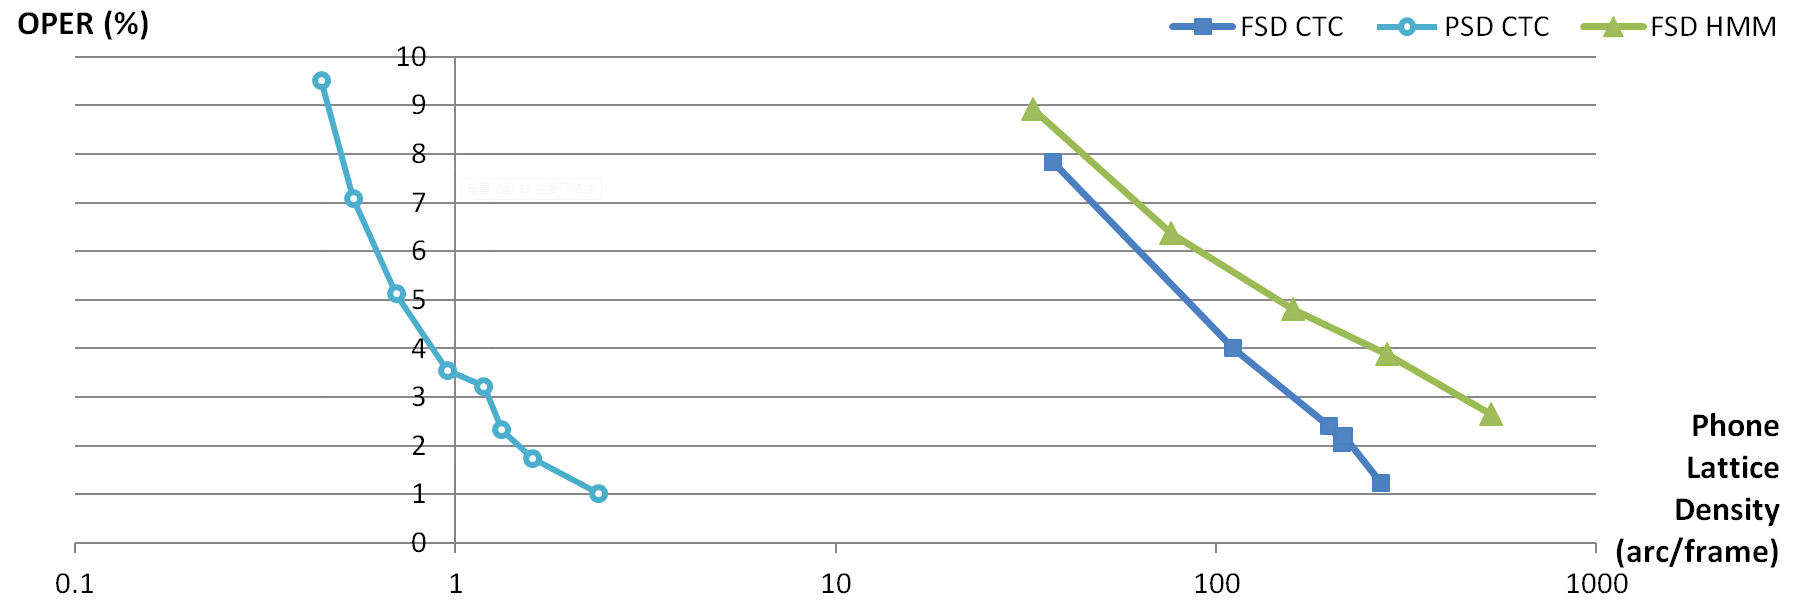
\includegraphics[width=\linewidth]{figure/OPER-latden.png}

        \caption{{\it OPER v.s. 词图密度在 FSD 和 LSD 中的比较}}
        \label{fig:OPER-latden}
      \end{figure}

图~\ref{fig:OPER-latden}表示了 OPER 和词图密度在不同解码配置结果中的对比,这包括由FSD和LSD生成的音素词图。
%Phone lattice generated from LSD is called LSD CTC lattice as in Section~\ref{sec:psd-ctc-lat} . Phone lattice generated from FSD is as the traditional method \cite{povey2012generating}.
在相似OPER情况下,对同一个CTC模型,LSD词图的大小比FSD词图小超过10倍。而LSD词图比HMM-DNN缩小的数量更大。产生这样现象的原因包括两方面:CTC更突出的后验概率特性而得到的紧致词图;LSD避免了词图生成过程的大量 $\tt blank$ 帧,而FSD则需要进行一些近似 \cite{ljolje1999efficient} 或进行词图裁剪\cite{povey2012generating}, 这将导致更大的搜索误差。
总结起来,在相同大小下,LSD CTC包含更多的音素声学信息。由于接下来的重点是比较FSD和LSD,因此我们仅罗列该部分结果。


\subsubsection{LSD CTC 词图及其生成的更好混淆网络}

%CTC model encodes the many-to-one function of $\mathcal{B}$ and results in peaky phonemic inference results.
%However, in FSD designed for HMM framework, phonemic output lasts for several frames because of  HMM modeling and state transition.  During generating word lattice, many-to-one function still needs to be done by merging same labels with similar time boundary but in a heuristic method (e.g. word lattice pruning).

为了构建混淆网络,需要先生成词级词图。 图~\ref{fig:OWER-latden} 表示了词级词图质量在FSD和LSD中的对比。
我们使用OWER进行比较。在图中纵轴,我们画出了 $1-\frac{OWER}{WER}$ 的值作为OWER相对下降值,以体现词图对最终质量改善的上限。从图中可以看出,在相同词图密度情况下,LSD系统总是得到更好的OWER。
      \begin{figure}[tbhp!]
        \centering
        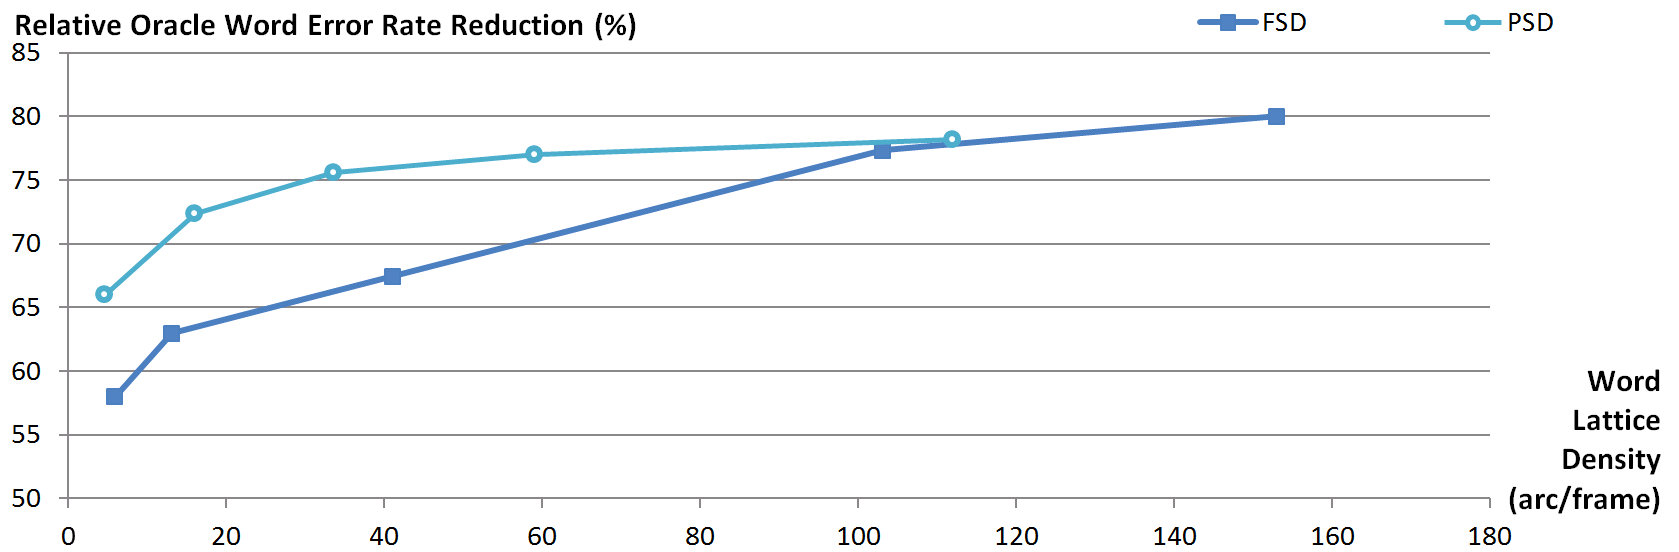
\includegraphics[width=\linewidth]{figure/OWER-latden.png}
        \caption{{\it 词图密度 v.s. 相对 OWER下降比例}}
        \label{fig:OWER-latden}
      \end{figure}
一旦词级词图被构建好,通过混淆网络的生成中的基于pivot的词聚类方法,相似时间边界的词边将会被合并在一起。因此,词级词图的时间边界的准确度对最终的混淆网络影响很大。为了分析词图的时间边界质量,我们提出最近pivot边界距离(NPBD),它定义为 $|b_{\tt arc}-b_{\tt cluster}|+|e_{\tt arc}-e_{\tt cluster}|$, 其中 $b_*$ 和 $e_*$ 为词的开始和结束时间边界, $\tt arc$ 是被对齐到最佳重叠 pivot 词 $\tt cluster$上的相应边。

%before CN cluster
      \begin{figure}[tbhp!]
        \centering
        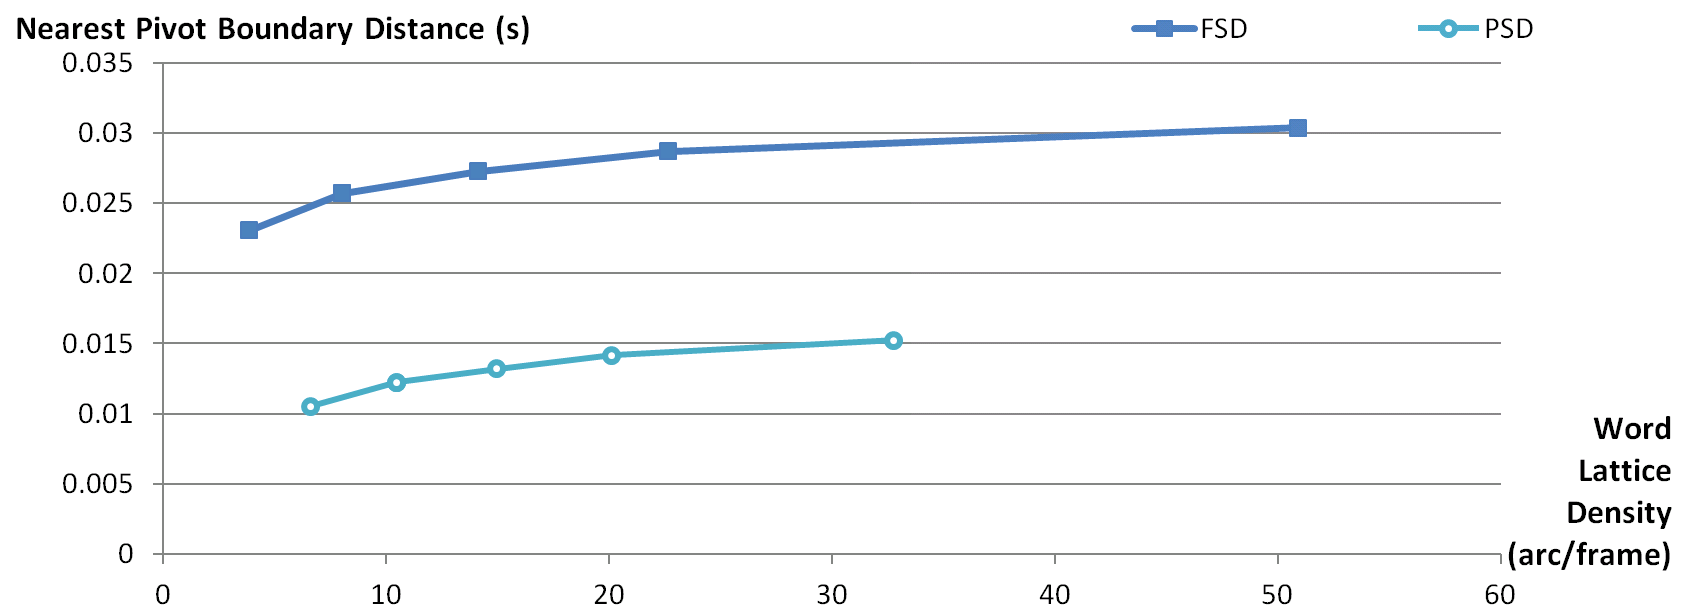
\includegraphics[width=\linewidth]{figure/bound-stable.png}
        \caption{{\it LSD和FSD的词边界稳定性}}
        \label{fig:bound-stable}
      \end{figure}
图~\ref{fig:bound-stable} 显示了LSD和FSD的NPBD。从图中可以看出LSD的词图的NPBD要明显小。换句话说,它的词边界更加稳定,由此可以得到更紧致的混淆网络。

%\subsubsection{Conversion Efficiency from Word Lattice to Confusion Network}
最后我们讨论了从词图到混淆网络的转换。图~\ref{fig:latden-cndepth} 显示了词图密度与混淆网络的深度之间的关系 \cite{hakkani2006beyond}。结果显示,即使在相似词图密度下,LSD的混淆网络往往包含更高的混淆网络深度,因此将得到更好的归一化项建模以及置信度建模方案。 

      \begin{figure}[tbhp!]
        \centering
        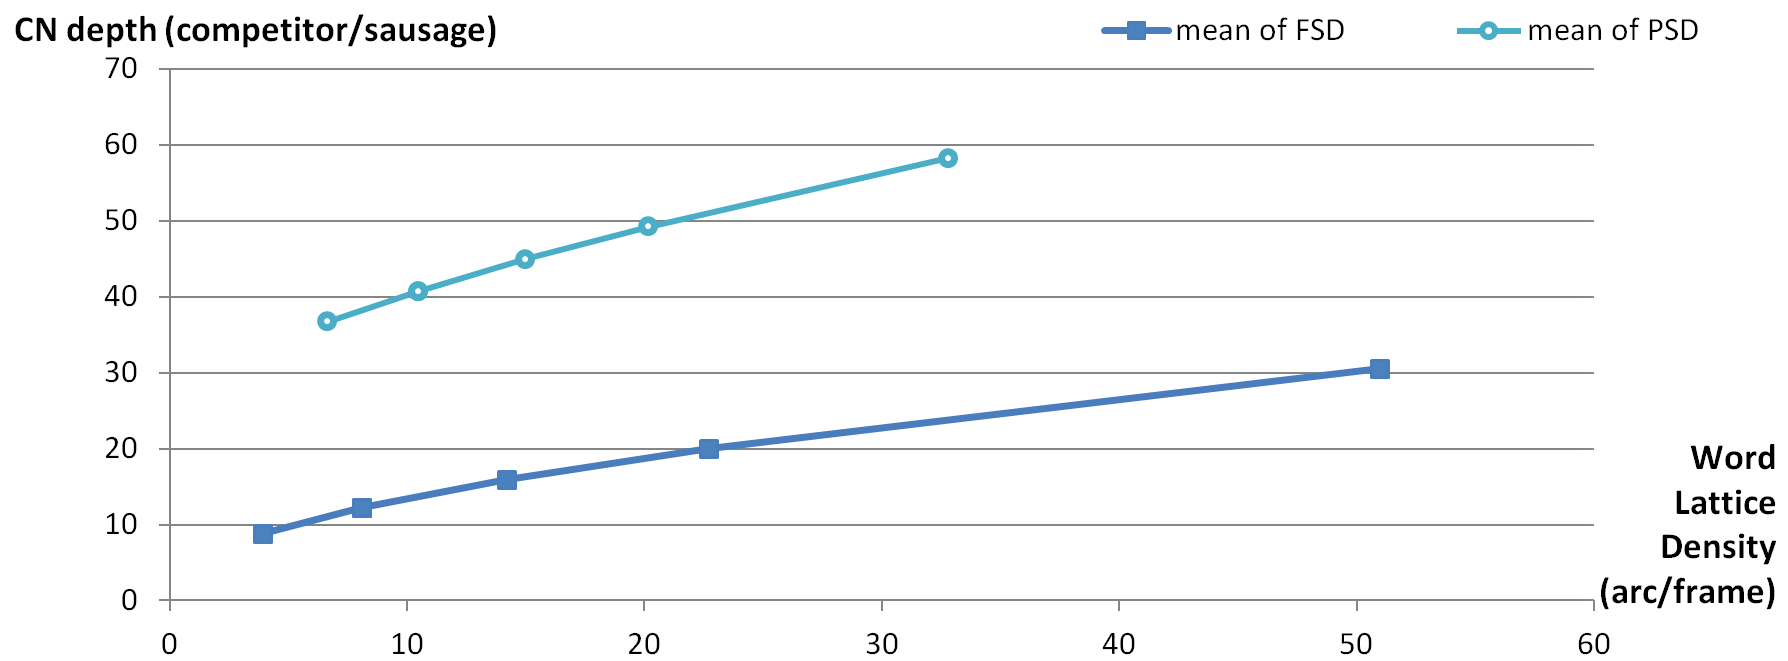
\includegraphics[width=\linewidth]{figure/latden-cndepth.png}

        \caption{{\it 词图密度 v.s. 混淆网络深度 }}
        \label{fig:latden-cndepth}

      \end{figure}


%\begin{itemize}
%    \item num of neighbors in each CN cluster(after arc clustering) from same size of lattice (in FSD \& LSD)
%    \item OWER v.s. CN size (compare FSD \& LSD)
%\end{itemize}



\subsection{置信度评估}

本章中我们比较上面讨论的混淆网络进一步得到置信度后的性能。为了补偿词图大小和对后验概率的过度估计,这里训练了一个决策树,来将所有概率映射到置信度分数上 \cite{evermann2000large}。 注意到,句子级置信度也可以由类似方法来得到。
我们使用上文提到的NCE来衡量词级置信度质量优劣。
     \begin{equation}\label{eq:nce}
    NCE=\frac{H(\mathbf{C})-H(\mathbf{C}|\mathbf{x})}{H(\mathbf{C})}
     \end{equation}
公式中 $H(\mathbf{C})$表示的是标注的序列的熵, $H(\mathbf{C}|\mathbf{x})$ 是置信度序列的熵。这是一个针对相比于总是提供平均分数的系统,其信息量增益的数量的指标。更高的NCE代表更好的系统。

\subsubsection{LSD 声学音素置信度}

表~\ref{tab:psd-conf}比较了所提出的LSD音素声学置信度与传统音素后验平均置信度。该传统方法 \cite{hu2013new}最初应用于HMM,并在本工作中拓展到 FSD的CTC 系统中 (表示为 {\em baseline}).  \ref{sec:psd-ac-conf} 提出的{\em peak-mean}, {\em peak-max}, {\em phone-mean}, {\em phone-conf} 
 等方案被表示为 {\tt PN1}, {\tt PN2}, {\tt PN3} and {\tt PC} 。
    \begin{table}[th]
    \caption{\label{tab:psd-conf} {\it 针对音素声学置信度的比较}}
        \centerline{
          \begin{tabular}{ c | c|  c ||  c }
            \hline
            \multirow{1}{*}{AM} &%\multicolumn{1}{|c||}{AM} &
            \multirow{1}{*}{Decoding} &
            \multirow{1}{*}{CM } &
            \multirow{1}{*}{NCE} \\
            %&&&\\
            \hline \hline
            DNN-HMM & FSD & baseline & 0.024 \\
            \hline
            \multirow{4}{*}{LSTM-CTC}&FSD&   baseline & 0.058\\
            \cline{2-4}
            &\multirow{3}{*}{LSD} &  $\tt PN1\oplus PN3$ & 0.105 \\
            &  & $\tt PN2\oplus PN3$ & 0.135 \\
            & &  $\tt PN2\oplus PN3\oplus PC$ & 0.141 \\
            \hline
          \end{tabular}
        }
      \end{table}
%fst-sp.ctc.sw1_fsh.o3g.kn_sp0_blk0_f_1ps_lconf10   FSD
结果显示,\cite{hu2013new}提出的音素声学置信度并不能被推广到词级。这是由于词边界的不确定性使得声学分数计算的时候存在重叠, 因此表现出了更差的结果。当该方法被使用在CTC模型时,词边界重叠问题得到了缓解,但是对于 {$\tt blank$} 概率的分配仍然存在混淆,比如对任意一个 {$\tt blank$} 是应该分配给前一个音素还是后一个音素存在不确定性。

在 LSD框架里,词边界和 {$\tt blank$} 分配问题都能够被解决,使得我们可以得到质量更好的置信度。同时当声学置信度和基于{\em phone-conf} 的置信度进行融合时,往往能取得最好的结果。因此在后续实验中,我们使用 $\tt PN2\oplus PN3\oplus PC$ 作为所提出的最优置信度。
%This is another superiority of LSD phonemic acoustic confidence because of effective usage of  information from {$\tt blank$} span.


\subsubsection{基于LSD的混淆网络的置信度}
%swb & CellPhone

%\subsubsection{Quality Comparison of Confidence Measures}
%word level NCE
表~\ref{tab:cn-conf} 比较了从LSD和FSD产生的混淆网络的置信度的质量。

    \begin{table}[th]
    \caption{\label{tab:cn-conf} {\it 基于混淆网络的置信度比较}}
        \centerline{
          \begin{tabular}{ c  |c|  c || c   }
            \hline
            \multirow{1}{*}{AM} &%\multicolumn{1}{|c||}{AM} &
            \multirow{1}{*}{Decoding} &
            \multirow{1}{*}{CM} &
            \multirow{1}{*}{NCE} \\
            %&&&\\
            \hline \hline
            DNN-HMM & FSD & \tt CN & 0.172 \\
            \hline
            \multirow{3}{*}{LSTM-CTC}&FSD&  \tt CN & 0.019\\
            \cline{2-4}
            &\multirow{2}{*}{LSD} &  \tt CN & 0.224 \\
            &  & \tt AC+CN & 0.230 \\
            \hline
          \end{tabular}
        }
      \end{table}
%kaldi get NCE
%/speechlab/users/zhc00/works/ctc/ctc-swb-ci-0621/kaldi_dec/get_nce.sh
%interpolation dir:
%/home/zhc00/new_fdecode_proj/conf_interpolation/README
%/home/zhc00/new_fdecode_proj/conf_interpolation/README_swb
%kaldi dnn get NCE
%from: zhc00@wuhan:/speechlab/users/zhc00/works/ctc/ctc-swb-ci-0621/dnn$ vi local/score_sclite_conf.sh
%zhc00@wuhan:/speechlab/users/zhc00/works/ctc/ctc-swb-ci-0621/dnn$ grep Sum exp/dnn_relu_asgd_svd/lang_decode_sw1_fsh.o3g.kn/eval2000_0.0833_10/score_*/eval2000.sw.ctm.filt.sys | awk '{print $1,$11,$14}'
%exp/dnn_relu_asgd_svd/lang_decode_sw1_fsh.o3g.kn/eval2000_0.0833_10/score_10_0.0/eval2000.sw.ctm.filt.sys:| 17.4 0.076
%exp/dnn_relu_asgd_svd/lang_decode_sw1_fsh.o3g.kn/eval2000_0.0833_10/score_12_0.0/eval2000.sw.ctm.filt.sys:| 17.0 0.139
%exp/dnn_relu_asgd_svd/lang_decode_sw1_fsh.o3g.kn/eval2000_0.0833_10/score_14_0.0/eval2000.sw.ctm.filt.sys:| 17.1 0.191
%exp/dnn_relu_asgd_svd/lang_decode_sw1_fsh.o3g.kn/eval2000_0.0833_10/score_16_0.0/eval2000.sw.ctm.filt.sys:| 17.7 0.209
%exp/dnn_relu_asgd_svd/lang_decode_sw1_fsh.o3g.kn/eval2000_0.0833_10/score_19_0.0/eval2000.sw.ctm.filt.sys:| 18.9 0.241

%fdecode result
%results/fst-sp.ctc.sw1_fsh.o3g.kn_sp0_blk2_f_1ps_nno_cn_np.nbest-10.1.car.0.0.5.eval2000.feat.fst_ctc_feat_v4/final.rst

该结果显示,虽然这种置信度在 CD-state-HMM 框架下效果较好 (与文献 \cite{evermann2000large}\cite{wessel2001confidence}一致), 但却不能够被直接应用到 CI-phone-CTC 模型上。这也是由于 {$\tt blank$} 的分配问题。
相反,基于CN的置信度可以被直接应用到LSD CTC音素词图框架并取得显著的性能改善。而且NCE还显著好于 CD-state-HMM 系统。我们相信这是因为CTC词图包含了更多的竞争信息,使得归一化项建模得更好,如图~\ref{fig:latden-cndepth}所示。

%CTC model encodes the many-to-one function of $\mathcal{B}$ and results in peaky phonemic inference results.
%However, in FSD designed for HMM framework, phonemic output lasts for several frames because of  HMM modeling and state transition.  During generating word lattice, many-to-one function still needs to be done by merging same labels with similar time boundary but in a heuristic method (e.g. word lattice pruning).

当LSD音素声学置信度 ($\tt PN2\oplus PN3\oplus PC$ 在表~\ref{tab:psd-conf}) 和基于CN的置信度相结合时 (表示为 {\tt AC+CN}), 性能得到了进一步改善。结果显示这两种置信度具有互补作用。我们认为第一种关注于局部而第二种则注重整个句子的评估。

%%%%%%%%%%%%%% unified %%%%%%%%%%%%%%%%


 \subsection{统一解码框架}
 \label{Sec:exp-kws}
 %meidi / wsj
 %EER & FScore
 在第一部分关键词检测任务中, 我们使用了398 个家居领域的关键词和相应的17332句测试集,这包括11789 个正例和 5543 个负例。表~\ref{tab:exp-kws-cm} 显示了不同方法之间的差别。

%RECALL: similar
%confidence v.s.: OK! google(bottum-up phonemic match method) & LSD lattice confidence & LSD acoustic confidence

    \begin{table}[th]

    \caption{\label{tab:exp-kws-cm} {\it KWS 任务}}

        \centerline{
          \begin{tabular}{  c|  c ||  c |c|c }
            \hline
            %\multirow{1}{*}{AM} &%\multicolumn{1}{|c||}{AM} &
            \multirow{1}{*}{CM } &
            \multirow{1}{*}{setup } &
            \multirow{1}{*}{EER(\%)} &
            \multirow{1}{*}{snt recall(\%)} &
            \multirow{1}{*}{PEA(\%)} \\
            %&&&\\
            \hline \hline
            %\multirow{2}{*}{DNN-HMM} & Phonemic  & - & 12.76 & -\\
            %\cline{2-5}
            %  & Hypothesis  & $\tt AX1$ & - & -\\
            %\hline
            Phonemic & $ \tt AC $  & 11.65 & 88.4 & 10 \\ %91.55
            \cline{1-5}
            \multirow{4}{*}{Hypothesis } &  $ \tt CN $ & 12.55 & 88.4 & 11\\
            \cline{2-5}
              & $\tt AX1$ & 11.60 & 88.0 & 10\\
              & $\tt AX2$ & 10.16 & 88.2 & 16\\
              & $\tt AX3$ & 10.10 & 88.2 & 15\\
            \hline
          \end{tabular}
        }

      \end{table}

 结果显示 $ \tt AC $ 效果比 $ \tt CN $好。原因是KWS中对搜索空间归一化项的建模非常薄弱,使得该部分估计不准。 本文所提出的附属归一化搜索空间可以减轻这样的问题,表中显示出了很大的改善。

除此之外,召回率显示本文提出的方法轻微影响了模型的准确度。考虑到在误唤醒方面显著的改善,这样的损失是可以接受的。

在效率方面,$ \tt CN $ 计算大约比 $ \tt AC $占据时间增加 10\% 。这方面来源于词图和混淆网络生成。虽然PEA比$ \tt AC $ 和 $ \tt CN $方法大, 但是总的时间仍然很小。这里的原因是由于使用了上文的LSD技术使得解码整体速度大幅加快\cite{Chen+2016}。

第二部分实验基于上下文的语音识别包含 13186 句语音助手语音,其中有7923 正例和 5263 反例。这些句子包括打电话,命令等。 这里的语法包括了所支持的说话方式和联系人信息。这里的负例包含领域内和领域外的错误。
 %dianhua
 %EER & FScore
 %RECALL: similar
    %confidence v.s.: LSD lattice confidence & LSD acoustic confidence

    \begin{table}[th]

    \caption{\label{tab:exp-grammar-cm} {\it 基于上下文的语音识别}}

        \centerline{
          \begin{tabular}{  c|  c ||  c |c|c }
            \hline
            %\multirow{1}{*}{AM} &%\multicolumn{1}{|c||}{AM} &
            \multirow{1}{*}{CM } &
            \multirow{1}{*}{setup } &
            \multirow{1}{*}{EER(\%)} &
            \multirow{1}{*}{snt recall(\%)} &
            \multirow{1}{*}{PEA(\%)}  \\
            %&&&\\
            \hline \hline
            %\multirow{2}{*}{DNN-HMM} & Phonemic  & - & 22.00 & -\\
            %\cline{2-5}
            %  & Hypothesis  & $\tt AX1$ & - & -\\
            %\hline
            %\multirow{4}{*}{LSTM-CTC}&
            Phonemic &   $ \tt AC $ & 19.86 & 87.4 & 38\\ %91.55
            \cline{1-5}
            \multirow{4}{*}{Hypothesis } &  $ \tt CN $  & 15.78  & 87.4 & 43 \\
            \cline{2-5}
              & $\tt AX1$ & 19.80  & 86.0 & 38 \\
              & $\tt AX2$ & 16.23   & 87.2 & 41\\
              & $\tt AX3$ & 16.12  & 87.2 & 40 \\
            \hline
          \end{tabular}
        }

      \end{table}

    表~\ref{tab:exp-grammar-cm} 给出了结果。在相比之前更大的搜索空间下, $ \tt CN $ 显著超越了 $ \tt AC $,因为 $ \tt AC $ 并没有使用其他的竞争信息,由此容易造成误唤醒。 $ \tt AX2 $ 和 $ \tt AX3 $ 类似于 $ \tt CN $。 原因是我们所提出的附属归一化搜索空间是针对ASR搜索空间的一个很好近似。 $\tt AX3$ 依然是性能最好的一个系统,我们将其用于下面的实验。

    关于效率,我们测试的框架对其基本没有影响。原因是与原来的搜索空间相比,我们提出的附属归一化搜索空间由于非常小,只会带来轻微影响。

    \subsection{大词汇连续语音识别}
    \label{Sec:exp-lvcsr}

    本章将在一个25小时左右的对话测试集中进行。解码使用一个118K词表的三元语言模型,其包含 {\em 1.9M} 个词对历史。
    %Table~\ref{tab:exp-lvcsr-cm} shows the result.

%RECALL: similar
    %confidence v.s.: LSD lattice confidence & LSD acoustic confidence

    \begin{table}[th]

    \caption{\label{tab:exp-lvcsr-cm} {\it LVCSR 任务}}

        \centerline{
          \begin{tabular}{  c|  c ||  c |c |c}
            \hline
            %\multirow{1}{*}{AM} &%\multicolumn{1}{|c||}{AM} &
            \multirow{1}{*}{CM } &
            \multirow{1}{*}{setup } &
            \multirow{1}{*}{NCE} &
            \multirow{1}{*}{CER(\%)} &
            \multirow{1}{*}{PEA(\%)} \\
            %&&&\\
            \hline \hline
            %\multirow{1}{*}{DNN-HMM} & Hypothesis  &  lattice based & - & -\\
            %\hline
            %\multirow{3}{*}{LSTM-CTC}&
            Phonemic &   $ \tt AC $  & 0.182& 10.2& 45  \\ %S-RTF 0.0072 RTF 0.016
            \cline{1-5}
            \multirow{2}{*}{Hypothesis } &  $ \tt CN $  & 0.302 & 10.2& 50 \\
            \cline{2-5}
              & $\tt AX3$ & 0.260 &10.1 & 46 \\
            \hline
          \end{tabular}
        }

      \end{table}

    与前面结论一致,$ \tt CN $ 性能好于 $ \tt AC $ 。 所提出的$ \tt AX3 $的结果比  $ \tt CN $差但差距不大。原因是对于LVCSR的搜索空间建模以及比较完整,附属归一化搜索空间并没有带来什么新的提升。另一方面基于效率考虑, $ \tt AX3 $使用最优路径来近似搜索空间,因此不如基于词图的建模更加完整。

    附属归一化搜索空间的系统的CER有轻微改善。我们认为是由于该搜索空间的存在将一些错误的搜索路径进行了剪枝,所以减少了插入和替换错误。关于效率,我们所提出的方法与之前一样影响不大。

    %Taking all three experiments into account, the proposed unified confidence measure and decoding framework using auxiliary normalization graph and phone synchronous decoding provides consistent performance and efficiency across varieties of ASR search space within the single framework.

    
\section{本章小结}
\label{chap:unify-sum}
由于不同ASR应用之间不同的搜索空间大小和效率要求,当前业界最优的置信度及其相应的解码算法在不同应用上具有不同架构。针对基于词图后验概率的置信度,计算量主要集中在词图部分的边缘概率计算过程。本章节中,我们首先改善了基于CTC的后验概率置信度方案;而后我们结合前面章节对解码的大幅加速和搜索空间的优化等工作,提出一系列针对不同应用的通用置信度,并尝试将不同应用中的语音识别推理过程统一到同一框架中。
%# -*- coding: utf-8-unix -*-
%%==================================================
%% conclusion.tex for SJTUThesis
%% Encoding: UTF-8
%%==================================================

\chapter{全文总结}
\label{chap:sum}

本论文围绕深度序列模型的建模和解码展开了一系列探索和研究,大幅改善了{\em 多种类}语音识别系统的{\em 精度}和{\em 速度}。
本论文的主要贡献在第\ref{chap:seqtrain}章、第\ref{chap:gpu}章、第\ref{chap:lsd}章、第\ref{chap:lsd-apply}章中介绍。第一个贡献是系统地研究序列建模方法,并应用到一系列非传统语音识别任务中,改善了系统精度,具体将在第\ref{chap:sum-kws}章总结;第二个贡献是提出并行的解码搜索算法并在GPU上实现开源该套算法,具体将在第\ref{chap:sum-gpu}章总结;第三个贡献是基于混淆区段($\tt blank$)建模,系统地提出了标签同步算法,具体将在第\ref{chap:sum-lsd}章总结。上述两项贡献从不同层面使得解码搜索技术得到了极大幅度加速。第四个贡献是将标签同步算法进一步应用到更多语音识别应用中,具体将在第\ref{chap:sum-unify}章总结。
除上述贡献外,作者在端到端建模和鲁棒语音识别建模中均有贡献,概述于第\ref{chap:intro2-e2e}章和第\ref{chap:intro2-pit}章。可能的后续工作展望在第\ref{chap:sum-future}章中总结。


\section{非传统识别任务的序列鉴别性训练}
\label{chap:sum-kws}

本论文针对关键词检测和多说话人重叠语音信号识别这两类任务提出了序列建模方案。

在本论文中,我们为深度学习的声学非固定关键词的关键词检测设计了相应的序列鉴别性训练方法,同时该方法也可以应用到固定关键词的关键词检测中。
%本文将序列概率的定义区分为序列条件似然度和序列后验概率,这包括两种序列模型: {\em 生成式序列模型} (GSM),比如HMM, 和 {\em 鉴别式序列模型} (DSM),比如 CTC。 对于GSM,序列鉴别性训练需要在序列上使用贝叶斯公式来通过序列条件似然度得到后验概率;而DSM则可以直接使用序列后验概率。
%
对这两种框架,竞争可能性的建模都是核心难题。本论文提出采用无词图鉴别性训练框架来解决这一问题:隐性使用音素或半词单元的语言模型来建模。

%总结我们的主要贡献包括:
%i) 针对生成式序列模型和鉴别式序列模型的序列鉴别性训练的第一个系统研究工作
%ii) 提出了一些新颖的办法来构建声学KWS的竞争可能性,以用于鉴别性训练。这些方法显著提升了关键词检测系统的性能。
%iii) 基于 LSD框架提出了高效的后处理方法,以便对音素混淆性进行建模。

近年来随着深度学习发展,将语音信号的增强和语音识别进行联合训练成为另一种新的趋势。这样做的好处包括:更好地利用序列信息进行训练;对模型前后模块进行联合调优以解决模型失配问题。
%
在单输出语音识别中,由于语音识别本身是一种序列分类和预测问题,序列级的准则将有助于改善系统性能。
而在鸡尾酒会问题中,对于单通道多说话人混叠语音识别系统,则又包含了说话人跟踪问题,也属于序列级问题。因此序列鉴别性准则将有助于这样的序列分类问题。
我们提出了一种传统鉴别性训练技术变种,它在进行鉴别性训练的同时,也抑制输出通道上说话人跟踪错误。
在多说话人重叠语音信号识别任务中,本文通过联合优化,迁移学习,序列鉴别性训练等方式,改善了原来语音分离、信号增强和语音识别的联合训练系统。


\section{面向大规模图搜索的并行维特比算法}
\label{chap:sum-gpu}

在本论文中,我们针对Kaldi开源工具包的推理搜索部分进行了一项重要扩展,以便使它能够支持图形处理芯片(GPU)上的WFST解码推理搜索。该框架可以显著加速现有推理搜索算法,特别是在基于深度序列学习的一系列模型上进行了验证。

这是一个通用的离线解码器,该解码器对语言模型和声学模型没有特别的限制,并且可以工作在各种架构的GPU上。
为了支持第二遍重打分和更丰富的后处理,我们的设计基于WFST解码和词图生成的架构~\cite{povey2012generating}。
针对设计中的几大难点,我们提出了如下解决方案:
我们将维特比算法中的令牌合并操作实现为一个GPU并行计算中的原子操作,以便减少维特比束剪枝算法中同步消耗;我们提出了动态负载均衡的方式以更高效地进行并行计算,提高其多线程之间的利用率;我们重新设计了基于GPU并行计算的精确的词图生成和剪枝算法,以便充分利用GPU的性能特点。


在Switchboard 上实验表明,我们所提出的方法在取得完全一致的1-best和词图质量情况下,可以得到3-15倍的加速,并在绝大部分GPU架构上进行了验证。除此之外,如果再进行多句子的并行处理,最终的加速比将达到46倍。
同时我们对这项工作进行了开源~\footnote{\url{https://github.com/chenzhehuai/kaldi/tree/gpu-decoder}},
它将与大多数Kaldi脚本相兼容。这项工作作为Kaldi工具包的一个扩展~\cite{povey2011kaldi},完整实现了基于GPU并行计算的WFST解码。



\section{基于标签同步解码的搜索空间优化}
\label{chap:sum-lsd}

基于端到端建模,
我们系统地提出了标签同步算法,其通过一系列方法使得搜索解码过程从逐帧同步变为标签同步,这包括使用高效的blank结构和后处理方法。该文提出的一系列通用方法在隐马尔科夫模型和连接时序分类模型上得到了验证。同时我们还介绍了将标签同步算法应用于序列到序列的端到端模型的方案,使之取得了更快和更好的模型收敛和模型准确度。


自动语音识别等序列标注任务的一个独特点是其对相邻帧的时序序列关联性建模。用于对相邻帧进行时序建模的主流序列模型包括隐马尔科夫模型(Hidden Markov Model, HMM)和连接时序分类模型(Connectionist Temporal Classification, CTC)。针对这些模型,当前主流的推理搜索方法是帧层面的维特比束搜索算法,该算法复杂度很高,限制了语音识别的广泛应用。深度学习的发展使得更强的上下文和历史建模成为可能。通过引入blanks(“空”)单元,端到端建模系统能直接预测标签在给定特征下的后验概率。

我们提出将特征层面的搜索过程改变为标签层面,即搜索空间是由不同历史的标签组成的,使得解码速率等于标签速率,从而小于特征速率。具体来说,在标签推理搜索阶段,对帧层面声学模型的输出增加一步后处理过程:i)判断当前帧是否存在标签输出;ii)若有,执行搜索过程;若无,则丢弃标签输出。因此该后处理过程可被看作是每个输出标签概率计算的近似。与传统方法相比,该方法的优势是搜索空间更小,且搜索过程被大大加速。
我们提出的一系列通用方法在隐马尔科夫模型和连接时序分类模型上得到了验证。
%

在实验部分,我们提出的系统取得了大幅度语音识别解码速度改善。


\section{标签同步解码的扩展应用}
\label{chap:sum-unify}
标签同步算法同时还能产生高质量的音素词图,称为LSD音素词图。基于LSD音素词图,本文进一步探讨标签同步解码算法的一些扩展应用。这包括关键词检测,多识别任务统一置信度框架,以及端到端语音识别。

在关键词检测中,我们基于前面章节介绍的LSD算法提出了一种高效的后处理算法,以解决音素混淆建模的问题。
在基于CTC的关键词检测中,虽然CTC是一个序列级准则,但是并没有对非关键词部分进行建模。因此该准则改善了关键词之间的鉴别性,但是没有改善关键词和非关键词之间的鉴别性。
本文将非关键词建模单元直接引入到建模当中。同时我们基于前述LSD算法得到的音素词图,提出了一套基于编辑距离的后处理算法以引入音素混淆性,使系统更加鲁棒。

连接时序分类模型 (CTC) 是一种目前比较主流的LVCSR模型。但是由于 $\tt blank$ 的引入,使得基于 CTC的词语级别的置信度 (CM) 并不能够被直接得到,特别是基于最主流的针对传统基于音素似然度归一化或者基于词图后验概率的混淆网络等方法。在前面提出的标签同步解码算法的基础上,我们进一步提出了两种置信度生成算法。更细致的研究显示这种基于CTC的音素词图是得到更好性能的关键所在。
在英文Switchboard 上的大词汇连续语音识别任务显示这里提出的LSD CTC 词图置信度算法可以显著改善原先传统的基于逐帧解码算法的CTC置信度或者 HMM模型的置信度。
%
另一方面由于不同ASR应用之间不同的搜索空间大小和效率要求,当前业界最优的置信度及其相应的解码算法在不同应用上具有不同架构,这些不同应用包括:关键词检测,基于上下文的语音识别和大词汇连续语音识别。针对基于词图后验概率的置信度,计算量主要集中在词图部分的边缘概率计算过程。本论文中,我们提出一系列针对不同应用的通用置信度,并尝试将不同应用中的语音识别推理搜索过程统一到同一框架中。
%
具体来说,我们提出了辅助归一化搜索空间的概念。我们尝试使用这样的搜索空间来建模所有ASR应用领域的置信度。 % and CM can be obtained in an unified framework
而针对这样做在低功耗设备上带来的挑战,我们采用基于CTC的标签同步解码\cite{Chen+2016} 来进行处理,由此带来了很大的效率改善。
最终这一统一高效的置信度框架被应用于目前主流的上述三种 ASR应用。

同时本论文还研究了将标签同步算法应用于直接建模输出序列形态学组合的端到端模型的方案。我们使用模块化训练的思想来改善端到端模型建模,使其更易于使用外在知识源来训练每一个端到端模型的子模块。值得注意的是,模型最后需要进行联合优化,因此最终在推理搜索阶段,模型仍然工作在端到端模式下。在实验部分,该章节系统一方面取得大幅度语音识别解码速度改善,另一方面在端到端建模上取得了更快和更好的模型收敛和模型准确度。


\section{后续工作展望}
\label{chap:sum-future}

本论文围绕深度学习背景下的序列建模和解码搜索技术展开了一系列探索和研究。进一步的后续研究方向包括:
\begin{itemize}
	\item 在本论文中,我们将并行计算的思想第一次应用到图搜索算法中。而自然语言处理中包含大量图搜索算法,将这种思路进一步推广和应用到其它任务中将会是非常有意义的研究。
	\item 在本论文中,我们基于端到端建模来简化传统语音识别中的搜索解码计算量。未来的研究包括两方面:一是进行更加端到端的建模,以进一步逐渐简化搜索解码;二是如何从深度学习的角度解释传统图搜索算法,由此提出更高效的深度学习模型来替代图搜索算法。
	\item 在本论文中,我们尝试采用深度学习语言模型和端到端建模来代替传统搜索空间的WFST框架。这样做的好处在于更快的搜索速度和更易于控制的搜索空间大小,由此可以使能更多和更灵活的端侧语音识别需求。未来想要完全实现该设想,则亟待更进一步的研究。
	\item 在本论文中,我们研究了关键词检测系统的序列鉴别性训练。采用其它的序列训练或序列准则以进一步改善关键词检测系统是一个有意义的研究话题,特别是尝试与本论文中提到的一些端到端建模方法相结合。
	\item 最后,将本论文提出的并行解码搜索技术与标签同步解码算法相结合,并推广到所提出的通用推理搜索和置信度框架中,得到一个速度极大幅提升,同时性能和置信度得到改善的通用系统,将会非常有意义。同时得益于速度的大幅提升和框架的简化,该方案具有进一步推广到端侧边缘计算的极大想象空间。
\end{itemize}




\appendix	% 使用英文字母对附录编号,重新定义附录中的公式、图图表编号样式
\renewcommand\theequation{\Alph{chapter}--\arabic{equation}}	
\renewcommand\thefigure{\Alph{chapter}--\arabic{figure}}
\renewcommand\thetable{\Alph{chapter}--\arabic{table}}
\renewcommand\thealgorithm{\Alph{chapter}--\arabic{algorithm}}

%% 附录内容,本科学位论文可以用翻译的文献替代。
%\include{tex/app_a}

\backmatter	% 文后无编号部分 

%% 参考资料
\printbibliography[heading=bibintoc]

%# -*- coding: utf-8-unix -*-
%%==================================================
%% pub.tex for SJTUThesis
%% Encoding: UTF-8
%%==================================================

\begin{publications}{99}
    \item\textsc{Chen H, Chan C~T}. {Acoustic cloaking in three dimensions using acoustic metamaterials}[J]. Applied Physics Letters, 2007, 91:183518.
    \item\textsc{Chen H, Wu B~I, Zhang B}, et al. {Electromagnetic Wave Interactions with a Metamaterial Cloak}[J]. Physical Review Letters, 2007, 99(6):63903.
\end{publications}
	  %% 发表论文
  %# -*- coding: utf-8-unix -*-
\begin{patents}{99}
    %\item 第一发明人,“永动机”,专利申请号202510149890.0
\item  voice recognition based decoding method and device PCT/CN2016/081334
\item  Sequence discriminative training based wakeup word device CN201710343427.5
\item  lattice rescoring system of deep learning based language model CN201810054749.2
\item  self-tagging, single direction and multi-view language modeling CN201710561261.4
\item  a decoding method and device of speech recognition CN201610221182.4
\item  adapative wakeup word method and device CN201610462976.X
\item  an audio recognition method and device CN201810025834.6
\item  a speech recognition method and device CN201810054315.2
\item  confidence measure based speech recognition method and device CN201710060942.2
\item  model compression and optimization of speech recognition device CN201810021903.6

\end{patents}
	  %% 申请专利
%% 致谢、发表论文、申请专利、参与项目、简历
%% 用于盲审的论文需隐去致谢、发表论文、申请专利、参与的项目
\makeatletter
\ifsjtu@review\relax\else
  %# -*- coding: utf-8-unix -*-
\begin{thanks}

  感谢所有测试和使用交大学位论文 \LaTeX 模板的同学!

  感谢那位最先制作出博士学位论文 \LaTeX 模板的交大物理系同学!

  感谢William Wang同学对模板移植做出的巨大贡献!

\end{thanks}
 	  %% 致谢
  %%# -*- coding: utf-8-unix -*-
%%==================================================
%% projects.tex for SJTUThesis
%% Encoding: UTF-8
%%==================================================

\begin{projects}{99}
    \item 973项目“XXX”
    \item 自然基金项目“XXX”
    \item 国防项目“XXX”
\end{projects}
  %% 参与的项目
% \include{tex/resume}	  %% 各人简历
\fi
\makeatother

\end{document}
